%%%%%%%% ICML 2023 EXAMPLE LATEX SUBMISSION FILE %%%%%%%%%%%%%%%%%

\documentclass{article}

% Recommended, but optional, packages for figures and better typesetting:
\usepackage{microtype}
\usepackage{graphicx}
\usepackage{subfigure}
\usepackage{booktabs} % for professional tables

% hyperref makes hyperlinks in the resulting PDF.
% If your build breaks (sometimes temporarily if a hyperlink spans a page)
% please comment out the following usepackage line and replace
% \usepackage{icml2023} with \usepackage[nohyperref]{icml2023} above.
\usepackage{hyperref}


% Attempt to make hyperref and algorithmic work together better:
\newcommand{\theHalgorithm}{\arabic{algorithm}}

% Use the following line for the initial blind version submitted for review:
% If accepted, instead use the following line for the camera-ready submission:
\usepackage[accepted]{icml2023}

% If accepted, instead use the following line for the camera-ready submission:
% \usepackage[accepted]{icml2023}

% For theorems and such
\usepackage{amsmath}
\usepackage{amssymb}
\usepackage{mathtools}
\usepackage{amsthm}
\usepackage{makecell}
\usepackage{float}

% if you use cleveref..
\usepackage[capitalize,noabbrev]{cleveref}

%%%%%%%%%%%%%%%%%%%%%%%%%%%%%%%%
% THEOREMS
%%%%%%%%%%%%%%%%%%%%%%%%%%%%%%%%
\theoremstyle{plain}
\newtheorem{theorem}{Theorem}[section]
\newtheorem{proposition}[theorem]{Proposition}
\newtheorem{lemma}[theorem]{Lemma}
\newtheorem{corollary}[theorem]{Corollary}
\theoremstyle{definition}
\newtheorem{definition}[theorem]{Definition}
\newtheorem{assumption}[theorem]{Assumption}
\theoremstyle{remark}
\newtheorem{remark}[theorem]{Remark}

% Todonotes is useful during development; simply uncomment the next line
%    and comment out the line below the next line to turn off comments
%\usepackage[disable,textsize=tiny]{todonotes}
\usepackage[textsize=tiny]{todonotes}


% The \icmltitle you define below is probably too long as a header.
% Therefore, a short form for the running title is supplied here:
\icmltitlerunning{Dividing and Conquering a BlackBox to a Mixture of Interpretable Models: Route, Interpret, Repeat}

\newcommand*\mystrut[1]{\vrule width0pt height0pt depth#1\relax}
\newcommand{\fix}{\marginpar{FIX}}
\newcommand{\new}{\marginpar{NEW}}
\newcommand\etal {{\it et al.}}
\newcommand\ie {{\it i.e., }}
\newcommand\st {{\it s.t., }}
\newcommand\eg {{\it e.g., }}
\newcommand\etc{{\it etc.}}
\newcommand\cf {{\it cf. }}
\newcommand\eq {{\it Eq.}}
\newcommand\ex {{ex.}}
\newcommand{\zerodisplayskips}{%
  \setlength{\abovedisplayskip}{0pt}%
  \setlength{\belowdisplayskip}{0pt}%
  \setlength{\abovedisplayshortskip}{0pt}%
  \setlength{\belowdisplayshortskip}{0pt}}
% \appto{\normalsize}{\zerodisplayskips}
% \appto{\small}{\zerodisplayskips}
% \appto{\footnotesize}{\zerodisplayskips}


\begin{document}

\twocolumn[
\icmltitle{Dividing and Conquering a BlackBox to a Mixture of Interpretable Models: Route, Interpret, Repeat}

% It is OKAY to include author information, even for blind
% submissions: the style file will automatically remove it for you
% unless you've provided the [accepted] option to the icml2023
% package.

% List of affiliations: The first argument should be a (short)
% identifier you will use later to specify author affiliations
% Academic affiliations should list Department, University, City, Region, Country
% Industry affiliations should list Company, City, Region, Country

% You can specify symbols, otherwise they are numbered in order.
% Ideally, you should not use this facility. Affiliations will be numbered
% in order of appearance and this is the preferred way.

\begin{icmlauthorlist}
\icmlauthor{Shantanu Ghosh}{bu}
\icmlauthor{Ke Yu}{pitt}
\icmlauthor{Forough Arabshahi}{meta}
\icmlauthor{Kayhan Batmanghelich}{bu}
\end{icmlauthorlist}

\icmlaffiliation{bu}{Department of Electrical and Computer Engineering, Boston University, MA, USA}
\icmlaffiliation{pitt}{Intelligent Systems Program, University of Pittsburgh, PA, USA}
\icmlaffiliation{meta}{MetaAI, MenloPark, CA, USA}

\icmlcorrespondingauthor{Shantanu Ghosh}{shawn24@bu.edu}

% You may provide any keywords that you
% find helpful for describing your paper; these are used to populate
% the "keywords" metadata in the PDF but will not be shown in the document
\icmlkeywords{Machine Learning, ICML}

\vskip 0.3in
]

% this must go after the closing bracket ] following \twocolumn[ ...

% This command actually creates the footnote in the first column
% listing the affiliations and the copyright notice.
% The command takes one argument, which is text to display at the start of the footnote.
% The \icmlEqualContribution command is standard text for equal contribution.
% Remove it (just {}) if you do not need this facility.

%\printAffiliationsAndNotice{}  % leave blank if no need to mention equal contribution
\printAffiliationsAndNotice{} % otherwise use the standard text.

\begin{abstract}


% ML model design either starts with an interpretable model or a Blackbox and explains it post hoc.
% Blackbox models are flexible but difficult to explain, while interpretable models are inherently explainable. 
% Yet, interpretable models require extensive ML knowledge and tend to be less flexible, potentially underperforming than their Blackbox equivalents. 
% This paper aims to blur the distinction between a post hoc explanation of a Blackbox and constructing interpretable models. 
% Beginning with a Blackbox, we iteratively \emph{carve out} a mixture of interpretable models and a \emph{residual network}. 
% The interpretable models identify a subset of samples and explain them using First Order Logic (FOL), providing basic reasoning on concepts from the Blackbox. 
% We route the remaining samples through a flexible residual. 
% We repeat the method on the residual network until all the interpretable models explain the desired proportion of data. 
% Our extensive experiments show that our \emph{route, interpret, and repeat} approach
% (1) identifies a richer diverse set of instance-specific concepts with high concept completeness via interpretable models by specializing in various subsets of data   without compromising in performance,
% (2) identifies the relatively ``harder'' samples to explain via residuals,
% (3) outperforms the interpretable by-design models by significant margins during test-time interventions,
% (4) can be used to fix the shortcut learned by the original Blackbox.


ML model design either starts with an interpretable model or a Blackbox and explains it post hoc. Blackbox models are flexible but difficult to explain, while interpretable models are inherently explainable. Yet, interpretable models require extensive ML knowledge and tend to be less flexible and underperforming than their Blackbox variants. This paper aims to blur the distinction between a post hoc explanation of a Blackbox and constructing interpretable models. 
% We hypothesize that a Blackbox model encodes several interpretable models, each applicable to different portions of data. 
Beginning with a Blackbox, we iteratively \emph{carve out} a mixture of interpretable experts (MoIE) and a \emph{residual network}. Each interpretable model specializes in a subset of samples and explains them using First Order Logic (FOL), providing basic reasoning on concepts from the Blackbox. We route the remaining samples through a flexible residual. We repeat the method on the residual network until all the interpretable models explain the desired proportion of data. Our extensive experiments show that our \emph{route, interpret, and repeat} approach (1) identifies a diverse set of instance-specific concepts with high concept completeness via MoIE without compromising in performance, (2) identifies the relatively ``harder'' samples to explain via residuals, (3) outperforms the interpretable by-design models by significant margins during test-time interventions, and (4) fixes the shortcut learned by the original Blackbox. The code for MoIE is
publicly available at: \url{https://github.com/batmanlab/ICML-2023-Route-interpret-repeat}.
\end{abstract}


\section{Introduction}
%  
Model explainability is essential in high-stakes applications of AI, such as healthcare. While BlackBox models (\eg Deep Learning) offer flexibility and modular design, post hoc explanation is prone to confirmation bias~\cite{wan2022explainability}, lack of fidelity to the original model~\cite{adebayo2018sanity}, and insufficient mechanistic explanation of the decision-making process~\cite{rudin2019stop}. Interpretable-by-design models do not suffer from those issues but tend to be less flexible than Blackbox models and demand substantial expertise to design and fine-tune. Using post hoc explanation or adopting an interpretable model is a mutually exclusive decision to be made at the initial phase of AI model design. This paper aims to blur the line on that dichotomous model design. 

The literature on post hoc explainable AI is extensive. The methods such as model attribution (\eg Saliency Map~\cite{simonyan2013deep, selvaraju2017grad}), counterfactual approach ~\cite{abid2021meaningfully, singla2019explanation}, and distillation methods~\cite{alharbi2021learning, cheng2020explaining} are examples of post hoc explainability approaches. Those methods either identify important features of input that contribute the most to the network's output~\cite{shrikumar2016not}, generate perturbation to the input that flips the network's output~\cite{samek2016evaluating}, \cite{montavon2018methods}, or estimate simpler functions that locally approximate the network output. The advantage of the post hoc explainability methods is that they do not compromise the flexibility and performance of the BlackBox. However, the post hoc explainability method suffers from several undesirable significant drawbacks, such as a lack of fidelity and mechanistic explanation of the network output~\cite{rudin2019stop}. Without a mechanistic explanation, recourse to a model's undesirable behavior is unclear. Interpretable models are alternative designs to the BlackBox model that do not suffer from many of those drawbacks. 

Interpretable models also have a long history in statistics and machine learning~\cite{letham2015interpretable, breiman1984classification}. Several families of interpretable models exist, such as the rule-based approach and generalized additive models~\cite{hastie1987generalized}. Many methods focus on tabular or categorical data and less on high-dimensional structured data such as images. Interpretable models for structured data rely mostly on projecting to a lower dimensional \emph{concept} or \emph{symbolic} space that is understandable for humans~\cite{koh2020concept}. Aside from a few exceptions ~\cite{ciravegna2021logic, barbiero2022entropy}, the current State-Of-The-Art (SOTA) design does not model the interaction between concepts and symbols, hence offering limited reasoning capabilities and less robustness. Furthermore, current designs are not as flexible as the Blackbox model, which may compromise the performance of such models. 


We aim to achieve the best of both worlds: the flexibility of the BlackBox and the mechanistic explainability of the interpretable models. The general idea is that a single interpretable model may not be sufficiently powerful to explain all samples, and several interpretable models might be hidden inside the Blackbox model. We construct a hybrid neuro-symbolic model by progressively \emph{carving out} a mixture of interpretable model and a \emph{residual network}. Our design identifies a subset of samples and \emph{routes} them through the interpretable models. The remaining samples are routed through a flexible residual network. We adopt First Order Logic (FOL) as the interpretable model's backbone, which provides basic reasoning on concepts retrieved from the BlackBox model. 
FOL is a logical function
that accepts predicates (concept presence/absent) as input and returns a True/False output being a
logical expression of the predicates. The logical expression, which is a set of AND, OR, Negative,
and parenthesis, can be written in the so-called Disjunctive Normal Form (DNF). DNF is a FOL logical formula composed of a disjunction (OR) of conjunctions (AND), known as the ``sum of products''.
On the residual network, we repeat the method until the proportion of data explained by the residual network falls below a desired threshold. The experimental results across various computer vision and medical imaging datasets reveal that our method accounts for the diversity of the explanation space and has minimal impact on the Blackbox's performance. Additionally, we apply our method's explanations to detect shortcuts in computer vision and successfully eliminate the bias from the Blackbox's representation.

\paragraph{Contributions}
% \begin{figure}[t]
% \centering
% \includegraphics[width=1\textwidth]{figures/Final/Local_explanation_motivation.pdf}
% \caption{The motivation of our work. All the plots correspond to detect a skin lesion as ``Malignant". In the left, (a) plot of the weights for each concepts by the fully interpretable model; (b) explanations by the interpretable model containing the concept \textit{sex} as it has the height weight, making the explanation too generic; (c) plot of the weights for each concepts by the expert4 using our method; (d) explanations by the expert4 using our method; (e) plot of the weights for each concepts by the expert5 using our method; (f) explanations by the expert5 using our method. From (c)-(f), we can see the expert model focuses on specific concept for specific samples.}
% \label{fig:motivation} 
% \end{figure}


Model explainability is essential in high-stakes applications of AI, \eg healthcare. While Blackbox models (\eg Deep Learning) offer flexibility and modular design, post hoc explanation is prone to confirmation bias~\cite{wan2022explainability}, lack of fidelity to the original model~\cite{adebayo2018sanity}, and insufficient mechanistic explanation of the decision-making process~\cite{rudin2019stop}. Interpretable-by-design models overcome those issues but tend to be less flexible than Blackbox models and demand substantial expertise to design. Using a post hoc explanation or adopting an inherently interpretable model is a mutually exclusive decision to be made at the initial phase of AI model design. This paper blurs the line on that dichotomous model design.

The literature on post hoc explanations is extensive. This includes model attributions (~\cite{simonyan2013deep, selvaraju2017grad}), counterfactual approaches ~\cite{abid2021meaningfully, singla2019explanation}, and distillation methods~\cite{alharbi2021learning, cheng2020explaining}. Those methods either identify key input features that contribute the most to the network's output~\cite{shrikumar2016not}, generate input perturbation to flip the network's output~\cite{samek2016evaluating, montavon2018methods}, or estimate simpler functions to approximate the network output locally. Post hoc methods preserve the flexibility and performance of the Blackbox but suffer from a lack of fidelity and mechanistic explanation of the network output~\cite{rudin2019stop}. Without a mechanistic explanation, recourse to a model's undesirable behavior is unclear. Interpretable models are alternative designs to the Blackbox without many such drawbacks. For example, modern interpretable methods highlight human understandable \emph{concepts} that contribute to the downstream prediction.

% Interpretable models also have a long history in statistics and machine learning~\cite{letham2015interpretable, breiman1984classification}. 
Several families of interpretable models exist for a long time, such as the rule-based approach and generalized additive models~\cite{hastie1987generalized, letham2015interpretable, breiman1984classification}. They primarily focus on tabular data. Such models for high-dimensional data (\eg images) primarily rely on projecting to a lower dimensional human understandable \emph{concept} or \emph{symbolic} space~\cite{koh2020concept} and predicting the output with an interpretable classifier. Despite their utility, the current State-Of-The-Art (SOTA)
%designs 1) require explicit concept annotation, 2) 
are limited in design; for example, they do not model the interaction between the concepts except for a few exceptions~\cite{ciravegna2021logic, barbiero2022entropy}, offering limited reasoning capabilities and robustness. Furthermore, if a portion of the samples does not fit the template design of the interpretable model, they do not offer any flexibility, compromising performance. 
%they are not as flexible as the Blackbox, thereby compromising the performance. 


\textbf{Our contributions}
We propose an interpretable method, aiming to achieve the best of both worlds: not sacrificing Blackbox performance similar to post hoc explainability while still providing actionable interpretation. We hypothesize that a Blackbox encodes several interpretable models, each applicable to a different portion of data. Thus, a single interpretable model may be insufficient to explain all samples. We construct a hybrid neuro-symbolic model by progressively \emph{carving out} a mixture of interpretable models and a \emph{residual network} from the given Blackbox. We coin the term \emph{expert} for each interpretable model, as they specialize over a subset of data. All the interpretable models are termed a ``Mixture of Interpretable Experts'' (MoIE). Our design identifies a subset of samples and \emph{routes} them through the interpretable models to explain the samples with FOL, providing basic reasoning on concepts from the Blackbox. The remaining samples are routed through a flexible residual network. 
On the residual network, we repeat the method until MoIE explains the desired proportion of data.
% FOL is a logical function
% that accepts predicates (concept presence/absent) as input and returns a True/False output being a
% logical expression of the predicates. The logical expression, which is a set of AND, OR, Negative,
% and parenthesis, can be written in the so-called Disjunctive Normal Form (DNF). DNF is a FOL logical formula composed of a disjunction (OR) of conjunctions (AND), known as the ``sum of products''. 
% % Why the solution is smart / Did it work.
We quantify the sufficiency of the identified concepts to explain the Blackbox’s prediction using the concept completeness score~\cite{yeh2019concept}.
Using FOL for interpretable models offers recourse when undesirable behavior is detected in the model. We provide an example of fixing a shortcut learning by modifying the FOL. FOL can be used in human-model interaction (not explored in this paper). Our method is the divide-and-conquer approach, where the instances covered by the residual network need progressively more complicated interpretable models. Such insight can be used to inspect the data and the model further. Finally, our model allows \emph{unexplainable} category of data, which is currently not allowed in the interpretable models.  
%The experimental results across computer vision and medical imaging datasets utilizing diverse architectures reveal that our method 
%1) is able to capture more meaningful instance-specific concepts  without sacrificing Blackbox's performance by qualitative and quantitative comparisons with the concept based interpretable-by-design and post hoc baselines, 
%2) does not require explicit concept annotation in training data, unlike most of the interpretable by design models,
%3) estimate ``harder'' to explain samples using the residuals,
%4) achieves significant performance boost during test-time interventions, 
%5) eliminates shortcut bias successfully from the Blackbox's representation.

% \begin{figure}[t]
% \centering
% \includegraphics[width=1\textwidth]{figures/Final/Local_explanation_motivation.pdf}
% \caption{The motivation of our work. All the plots correspond to detect a skin lesion as ``Malignant". In the left, (a) plot of the weights for each concepts by the fully interpretable model; (b) explanations by the interpretable model containing the concept \textit{sex} as it has the height weight, making the explanation too generic; (c) plot of the weights for each concepts by the expert4 using our method; (d) explanations by the expert4 using our method; (e) plot of the weights for each concepts by the expert5 using our method; (f) explanations by the expert5 using our method. From (c)-(f), we can see the expert model focuses on specific concept for specific samples.}
% \label{fig:motivation} 
% \end{figure}

% \section{Related work}
% % Post hoc methods
% Saliency cam grad cam
% attribution lime shap l2x

% interpretable models
% early GAM - tabular data
% CBM no composability
% E-LENS FOL

\textbf{Post hoc explanations:} \cite{simonyan2013deep, selvaraju2017grad, smilkov2017smoothgrad} discuss the post hoc explanation method using saliency maps to explain a convolution neural network, highlighting the pixels in the input images that contributed to the network's prediction. \cite{adebayo2018sanity, kindermans2019reliability}  demonstrates that the saliency maps highlight the correct regions in the image even though the backbone's representation was arbitrarily perturbed. Additionally, in LIME~\cite{ribeiro2016should}, given a superpixel, a surrogate linear function attempts to learn the prediction of the Blackbox surrounding that superpixel. SHAP \cite{SHAP} utilizes a game-theoretic strategy called SHAPLY values to estimate the Blackbox's prediction by considering all the permutations of adding and removing a specific feature to determine its importance in the final prediction. Regarding pixel intensities, the explanations do not correspond to the high-level, human-interpretable \emph{concepts}. In this paper, we provide the post hoc explanation of the Blackbox in terms of the interpretable concepts, rather than the pixel intensities.

% \textbf{Concept-based interpretable models}: 
% In this class, the researchers try to design inherently interpretable models to eliminate the  requirement for post hoc explanations. In the literature, we find interpretable models in Generalized Additive Models (GAM)~\cite{hastie1987generalized}, or on logic formulas, as in Decision Trees~\cite{breiman1984classification} or Bayesian Rule Lists (BRL)~\cite{letham2015interpretable}. 
% % GAMs overcome the linearity assumption of linear regression by learning target categories disjointly from each feature. 
% However, most of these methods work well in categorical datasets rather than continuous data such as images. Additionally,~\cite{chen2019looks} introduces a ``case-based reasoning'' technique, known as ``ProtoPNet''. Here, the authors first dissect an image in Prototypical parts and then classifies by combining evidence from the pre-defined prototypes. This method is highly sensitive to the choice of prototypes and the distance metric used to compare with the prototype. So instead of using any prototypes, our proposed method uses human understandable concepts to build the mixture of interpretable models.
\textbf{Concept-based interpretable models:}
Recently, CBM~\cite{koh2020concept}, based on the interpretable-by-design principle, leverages the weak annotations of visual attributes to predict the high-level human-comprehensible concepts~\cite{kim2017interpretability} from images and then the class labels from the discovered concepts. A concept decoder is used in the antehoc model~\cite{sarkar2021inducing} to simultaneously reconstruct the image from the concepts to ensure the the semantics of the input image from the concepts, specifically aiming for unsupervised concept discovery. Instead of learning scalar concepts in the bottleneck, CEM~\cite{zarlenga2022concept} uses high dimensional concept embeddings to allow extra supervised learning capacity. Later,PCBM ~\cite{yuksekgonul2022post} learns the concepts from the embeddings of a trained Blackbox and uses an interpretable classifier for classification. Also, they propose the Hybrid-Post-hoc-concept-based model (PCBM-h) to replicate the performance of the Blackbox. Yet, they do not explain how the final classifier composes those concepts for prediction. An inherently interpretable ELL~\cite{barbiero2022entropy} addresses this gap by introducing an entropy-based classifier for the downstream classification and providing explanations in terms of FOL using the concepts. However, all these methods 1) employ a single interpretable model to explain a Blackbox, failing to apprehend different forms of explanations for different samples and offering generic explanations for all samples of a class 2) did not quantify if the identified concepts is faithful to the Blackbox's prediction. We introduce MoIE to address this issue, utilizing Blackbox's flexibility to identify meaningful instance-specific concepts with high concept completeness to offer a local explanation using FOL. In addition, we learn the residuals in each iteration for the samples not covered by the associated interpretable model, whereas PCBM-h trains the residual for all samples.

\textbf{Shortcut learning:}
"Shortcuts'' are defined when a predictor relies on easy-to-learn spurious correlations between the inputs and the target~\cite{geirhos2020shortcut}. Learning shortcuts can broadly be categorized either in example difficulty estimation~\cite{lalor2018understanding, hooker2019compressed, agarwal2022estimating} or monitoring training dynamics~\cite{hu2020surprising, feng2021phases, rabanser2022selective}. Unlike these methods, MoIE discovers shortcut using the high level concepts in FOL explanation of the Blackbox's prediction of a sample, routed through an interpretable model and eliminate it using MDN \cite{lu2021metadata}.


\section{Method}
\label{sec:method}
% 
\textbf{Notation and learning the concepts:} 
Assume $f^0: \mathcal{X} \rightarrow \mathcal{Y}$ is a pre-trained Blackbox predicting the output from the input image. Also, $\displaystyle f^0(.) =  h^0 \circ \Phi(.) $. Here, $ \Phi: \mathcal{X} \rightarrow R^l $ is the image embeddings and $ h^0: R^l \rightarrow \mathcal{Y}$ is the classifier, classifying the output $\mathcal{Y}$ using the embeddings, $\Phi$. Our approach is applicable for both datasets with and without human-interpretable concept annotations. For datasets with the concept annotation $\mathcal{C} \in \mathbb{R}^{N_c}$ ($N_c$ being the number of concepts per image $\mathcal{X}$), we learn $t: R^l \rightarrow\mathcal{C}$ to classify the concepts using the embeddings. Per this definition, $t$ outputs a scalar value $c$ representing a single concept for each input image. 
%We adopt the concept learning strategy in PosthocCBM (PCBM)~\cite{yuksekgonul2022post} for datasets without concept annotation. 
%Specifically, we leverage a set of image embeddings with the concept being present and absent. Next, we learn a linear SVM to construct the concept activation matrix~\cite{kim2017interpretability} as $\boldsymbol{Q} \in\mathbb{R}^{N_c \times l}$. 
Finally we estimate the concept value as $c = \frac{<\Phi(x), q^i>}{||q_i||_2^2}$ $ \in \mathbb{R}$ utilizing each row $\boldsymbol{q^i}$ of $\boldsymbol{Q}$. Thus, the complete tuple of $j^{th}$ sample is $\{x_j, y_j, c_j\}$, denoting the image, label, and learned concept vector, respectively.

\textbf{Method Overview:} 
Figure \ref{fig:Schematic} summarizes our approach. We iteratively carve out an interpretable model from the given Blackbox. Each iteration yields an interpretable model (the downward grey paths in Figure \ref{fig:Schematic}) and a residual (the straightforward black paths in Figure \ref{fig:Schematic}).
We start with the initial Blackbox $f^0$.
At iteration $k$, we distill the Blackbox from the previous iteration $f^{k-1}$ into a neuro-symbolic interpretable model, $\displaystyle g^{k}: \mathcal{C} \rightarrow \mathcal{Y}$. Our $g$ is flexible enough to be any interpretable models \eg logistic classifier~\cite{yuksekgonul2022post, koh2020concept, barbiero2022entropy}. The \emph{residual} $r^k =f^{k-1} - g^k$ emphasizes the portion of $f^{k-1}$ that $g^k$cannot explain. We then approximate $r^k$ with $f^{k} = h^k(\Phi(.))$. $f^k$ will be the Blackbox for the subsequent iterations and be explained by the respective interpretable model. 
% Due to computational reasons, we only finetune $h^{k}$ to optimize for $r^k$. 
A learnable gating mechanism, denoted by $\pi^k : \mathcal{C} \rightarrow \{0,1\}$ (shown as the \emph{selector} in figure \ref{fig:Schematic}) routes an input sample towards either $g^k$ or $r^k$.
% In order to learn $\pi^k$, we use simple backpropagation while learning $g^k$. A
The thickness of the lines in Figure \ref{fig:Schematic} represents the samples covered by the interpretable models (grey line) and the residuals (black line). 
% Our method is designed such that it leaves a little number of samples for the last residual blackbox.
With every iteration, the cumulative coverage of the interpretable models increases, but the residual decreases. We name our method \emph{route, interpret} and \emph{repeat}.

\subsection{Neuro-Symbolic Knowledge Distillation}
Knowledge distillation in our method involves 3 parts: (1) a series of trainable selectors ,\emph{routing} each sample through the interpretable models and the residual networks, (2) A sequence of learnable neuro-symbolic interpretable models, each providing FOL explanations to \emph {interpret} the Blackbox, and (3) \emph{repeating} with Residuals for the samples that cannot be explained with their interpretable counterparts. 
We detail each component below.

\begin{figure}[h]
% \vskip 0.2in
\centering
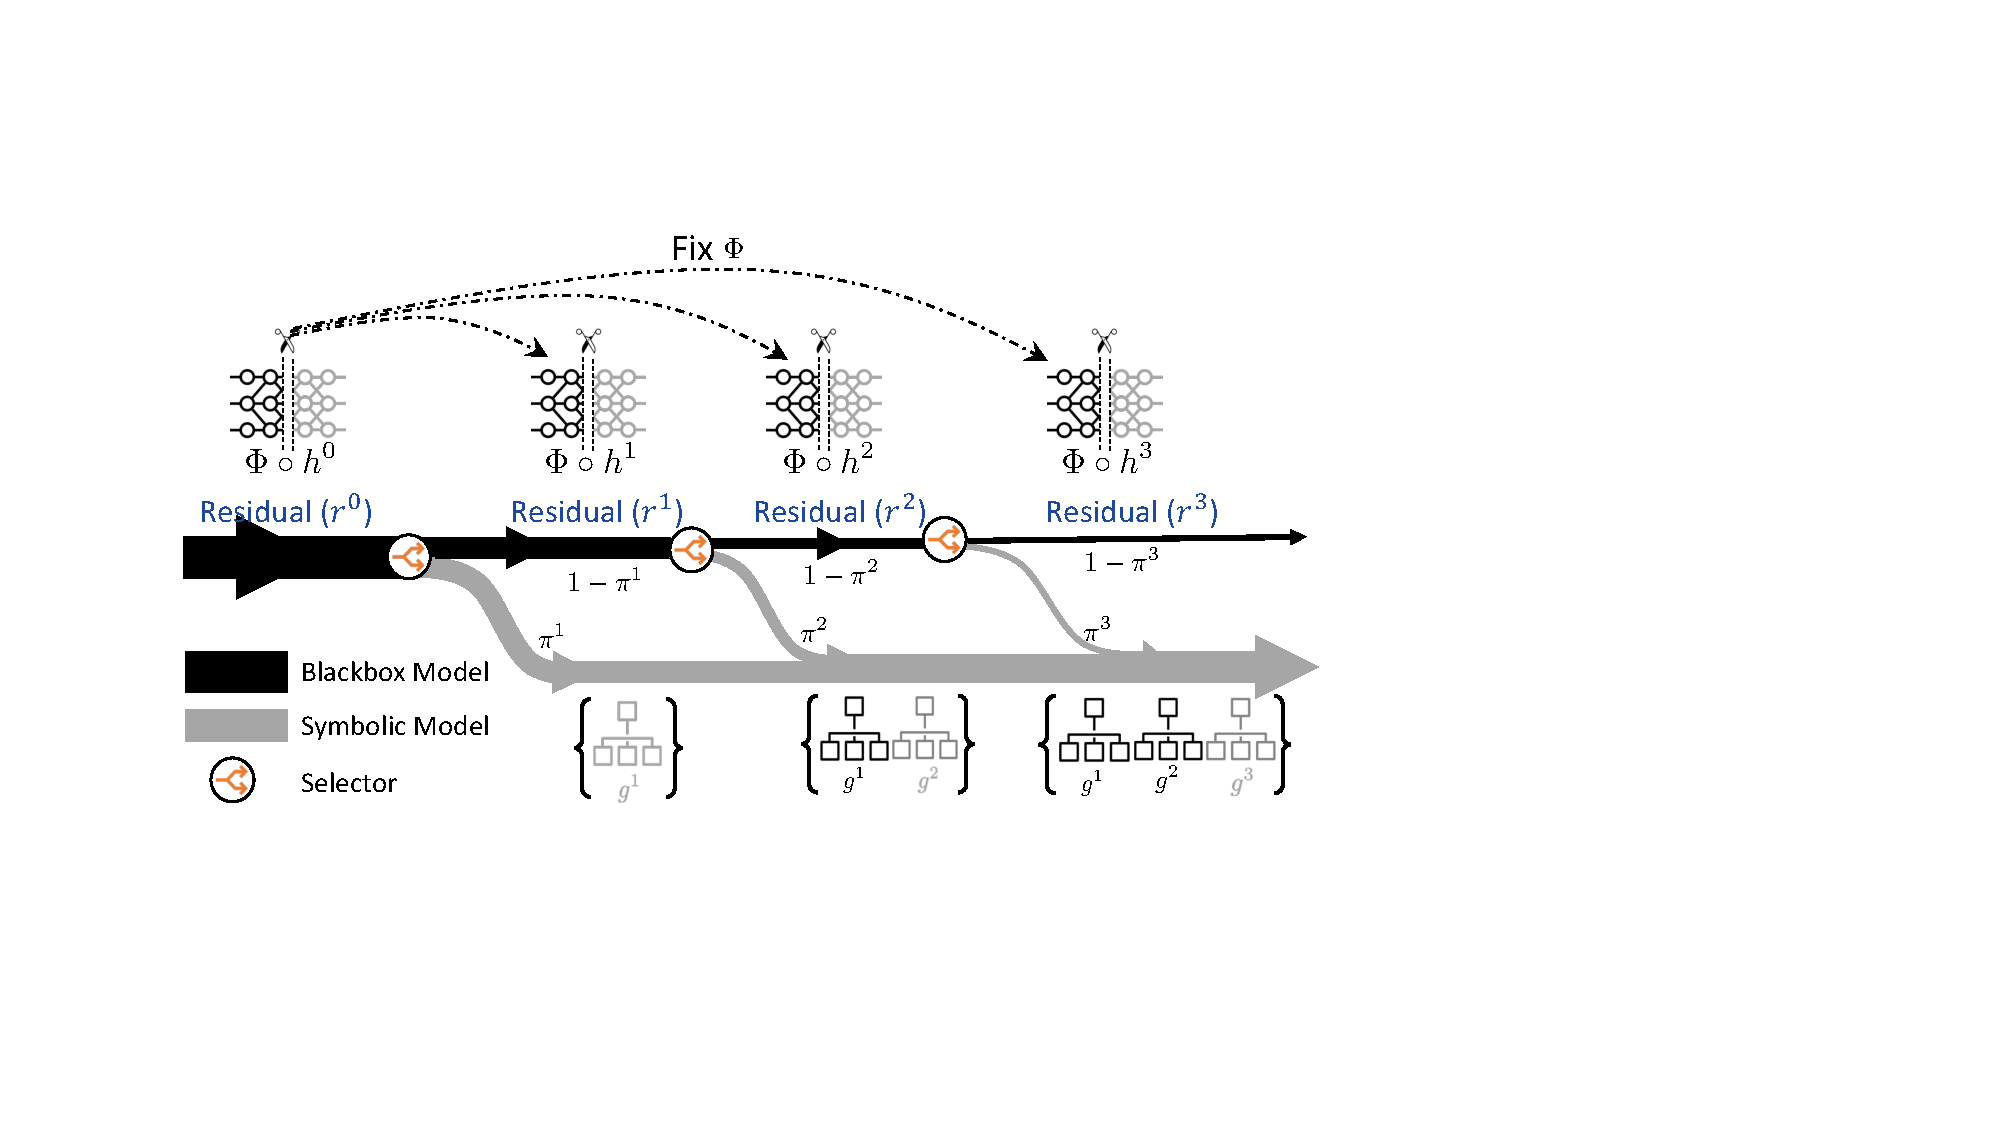
\includegraphics[width=\columnwidth]{figures/main/schematic.pdf}
\vskip -3pt
\caption{Schematic view of \emph{route, interpret} and \emph{repeat}. At iteration $k$, the selector \emph{routes} each sample either towards the interpretable model $g^k$ (to \emph{interpret}) with probability $\pi^k(.)$ or the residual $r^k = f^{k-1} - g^k$ with probability $1-\pi^k(.)$ (to \emph{repeat} in the further iterations). $f^{k-1}$ is the Blackbox of the $(k-1)^{th}$ iteration. $g^k$ generates FOL-based explanations for the samples it covers. Otherwise, the selector routes through the next step until it either goes through a subsequent interpretable model or reaches the last residual. Also, components in black and grey indicate the fixed and trainable modules in our model respectively. }
\label{fig:Schematic} 
\vskip -0.1in
\end{figure}

\subsubsection{The selector function}
As the first step of our method, the selector $\pi^k$ \emph{routes} the $j^{th}$ sample through the interpretable model $g^k$ or residual $r^k$ with probability $\displaystyle \pi^k(\boldsymbol{c_j})$ and $\displaystyle 1 - \pi^k(\boldsymbol{c_j})$ respectively, where $k$ $\in [0,K]$, with $K$ being the number of iterations.
We define the empirical coverage of the $\displaystyle k^{th}$ iteration as $\vspace{-0.08pt} \zeta(\pi^k) = \frac{1}{m}\sum_{j = 1} ^ m \pi^k(\boldsymbol{c_j}) \vspace{-0.081pt}$, the empirical mean of the samples selected by the selector for the associated interpretable model $\displaystyle g^k$, with $\displaystyle m$ being the total number of samples in the training set. Thus, the entire selective risk is:

\vskip -7.5pt
\begin{equation}
\label{equ: emp_risk}
\mathcal{R}^k(\displaystyle \pi^k, \displaystyle g^k) = \frac{\frac{1}{m}\sum_{j=1}^m\mathcal{L}_{(g^k, \pi^k)}^k\big(\boldsymbol{x_j}, \boldsymbol{c_j}\big)}{\zeta(\pi^k)} ,
\end{equation}
\vskip 2pt

where $\mathcal{L}_{(g^k, \pi^k)}^k$ is the optimization loss used to learn $\displaystyle g^k$ and $\displaystyle \pi^k$ together, discussed in section \ref{ns-optimization}. For a given coverage of $\displaystyle \tau^k \in (0, 1]$, we solve the following optimization problem:

\vskip -7.5pt
\begin{align}
\label{equ: optimization_g}
\theta_{s^k}^*, \theta_{g^k}^* = & \operatorname*{arg\,min}_{\theta_{s^k}, \theta_{g^k}} \mathcal{R}^k\Big(\pi^k(.; \theta_{s^k}), \displaystyle g^k(.; \theta_{g^k}) \Big) \nonumber \\ 
&\text{s.t.} ~~~ \zeta\big(\pi^k(.; \theta_{s^k})\big) \geq \tau^k,
\end{align}
\vskip 2pt

where $\theta_{s^k}^*, \theta_{g^k}^*$ are the optimal parameters at iteration $k$ for the selector $\pi^k$ and the interpretable model $g^k$ respectively. In this work, $\pi$s' of different iterations are neural networks with sigmoid activation. At inference time, the selector routes the $j^{th}$ sample with concept vector $\boldsymbol{c_j}$ to $\displaystyle g^k$ if and only if $\pi^k(\boldsymbol{c}_j)\geq 0.5$ for $k \in [0,K]$.

\subsubsection{Neuro-Symbolic interpretable models}
\label{ns-optimization}
In this stage, we design interpretable model $\displaystyle g^k$ of $k^{th}$ iteration  to \emph{interpret} the Blackbox $\displaystyle f^{k - 1}$ from the previous $(k-1)^{th}$ iteration by optimizing the following loss function:
\begin{equation}
\label{equ: g_k}
\resizebox{0.47\textwidth}{!}{$
\mathcal{L}_{(g^k, \pi^k)}^k\big(\boldsymbol{x_j}, \boldsymbol{c_j}\big) = \underbrace{\mystrut{2.6ex}\ell\Big(f^{k - 1}(\boldsymbol{x_j}), g^k(\boldsymbol{c_j})\Big)\pi^k(c_j) }_{\substack{\text{trainable component} \\ \text{for current iteration $k$}}}\underbrace{\prod_{i=1} ^{k - 1}\big(1 - \pi^i(\boldsymbol{c_j})\big)}_{\substack{\text{fixed component trained} \\ \text{in the previous iterations}}},
$}
\end{equation}

where the term $\pi^k(\boldsymbol{c_j})\prod_{i=1} ^{k - 1}\big(1 - \pi^i(\boldsymbol{c_j}) \big)$ denotes the probability of $j^{th}$ sample being routed through the interpretable model $g^k$. It is the probability of the sample going through the residuals for all the previous iterations from $0$ through $k-1$ (\ie $\prod_{i=1} ^{k - 1}\big(1 - \pi^i(\boldsymbol{c_j}) \big)$\big) times the probability of going through the interpretable model at iteration $k$ \big(\ie $\pi^k(\boldsymbol{c_j})$\big). 
Refer to Figure~\ref{fig:Schematic} for an illustration. We learn $\pi^1, \dots \pi^{k - 1}$ in the prior iterations and are not trainable at iteration $k$. As each interpretable model $g^k$ specializes in explaining a specific subset of samples (denoted by coverage $\tau$), we refer to it as an \emph{expert}. We use SelectiveNet's ~\cite{geifman2019selectivenet}  optimization method to optimize equation \ref{equ: optimization_g} since selectors need a rejection mechanism to route samples through residuals. Appendix \ref{app:loss} details the optimization procedure in equation \ref{equ: g_k}. We refer to the interpretable experts of all the iterations as a ``Mixture of Interpretable Experts'' (MoIE) cumulatively after training. Furthermore, we utilize Entropy-based linear layer neural network (ELL)~\cite{barbiero2022entropy} as the interpretable symbolic model $g$ to construct First Order Logic (FOL) explanations of a given prediction.

\subsubsection{The Residuals}
The last step is to \emph{repeat} with the residual $r^k$, as $\displaystyle r^k(\boldsymbol{x_j},\boldsymbol{c_j}) = f^{k - 1}(\boldsymbol{x_j}) - g^k(\boldsymbol{c_j})$.
We train $f^k = h^k\big(\Phi(.)\big)$ to approximate the residual $r^k$, creating a new Blackbox $f^k$ for the next iteration $(k+1$). This step is necessary to specialize $\displaystyle f^k$ over samples not covered by $g^k$. Optimizing the following loss function yields $\displaystyle f^k$ for the $\displaystyle k^{th}$ iteration:
\begin{equation}
\label{equ: residual}
\mathcal{L}_f^k(\boldsymbol{x_j}, \boldsymbol{c_j}) = \underbrace{\mystrut{2.6ex}\ell\big(r^k(\boldsymbol{x_j}, \boldsymbol{c_j}), f^k(\boldsymbol{x_j})\big)}_{\substack{\text{trainable component} \\ \text{for iteration $k$}}} \underbrace{\mystrut{2.6ex}\prod_{i=1} ^{k}\big(1 - \pi^i(\boldsymbol{c_j})\big)}_{\substack{\text{non-trainable component} \\ \text{for iteration $k$}}} 
\end{equation}

% \underbrace{\mystrut{2.6ex}\ell\big(f^{k - 1}(\boldsymbol{x_j}), g^k(\boldsymbol{c_j})\big)\pi^k(c_j) }_{\substack{\text{trainable component} \\ \text{from current iteration}}}
Notice that we fix the embedding $\displaystyle \Phi(.)$ for all the iterations. Due to computational overhead, we only finetune the last few layers of the Blackbox ($h^k$) to train $f^k$.
At the final iteration $K$, our method produces a MoIE and a Residual, explaining the interpretable and uninterpretable components of the initial Blackbox $f^0$, respectively. Appendix \ref{app:algo} describes the training procedure of our model, the extraction of FOL and the architecture of our model at inference.


\textbf{Selecting number of iterations $K$:} We follow two principles to select the number of iterations $K$ as a stopping criterion: 1) Each expert should have enough data to be trained reliably (
coverage $\zeta^k$). If an expert covers insufficient samples, we stop the process. 2) If the final residual ($r^K$) underperforms a threshold, it is not reliable to distill from the Blackbox. We stop the procedure to ensure the overall accuracy is maintained.


\textbf{Notation:} 
Assume we have a dataset \{$\mathcal{X}$, $\mathcal{Y}$, $\mathcal{C}$\}, where $\mathcal{X}$, $\mathcal{Y}$, and $\mathcal{C}$ are the input images, class labels, and human interpretable attributes, respectively. $\displaystyle f^0:  \mathcal{X} \rightarrow \mathcal{Y}$, is our pre-trained initial Blackbox model. We assume that $\displaystyle f^0$ is a composition $\displaystyle h^0 \circ \Phi $, where $\displaystyle \Phi: \mathcal{X} \rightarrow \mathbb{R}^l $ is the  image embeddings and $\displaystyle h^0: \mathbb{R}^l \rightarrow \mathcal{Y}$ is a transformation from the embeddings, $\Phi$, to the class labels. We denote the learnable function $\displaystyle t: \mathbb{R}^l \rightarrow\mathcal{C}$, projecting the image embeddings to the concept space.
% We denote the learnable function $\displaystyle t: \R^l \rightarrow\mathcal{C}$, projecting the image representations to the concept space.  
The concept space is the space spanned by the attributes $\mathcal{C}$. Thus, function $t$ outputs a scalar value representing a concept for each input image. 

\textbf{Method Overview:} 
\cref{fig:Schematic} summarizes our approach. We iteratively carve out an interpretable model from the given Blackbox. Each iteration yields an interpretable model (the downward grey paths in~\cref{fig:Schematic}) and a residual (the straightforward black paths in~\cref{fig:Schematic}).
We start with the initial Blackbox $f^0$.
At iteration $k$, we distill the Blackbox from the previous iteration $f^{k-1}$ into a neuro-symbolic interpretable model, $\displaystyle g^{k}: \mathcal{C} \rightarrow \mathcal{Y}$. Our $g$ is flexible enough to be any interpretable models~\cite{yuksekgonul2022post, koh2020concept, barbiero2022entropy}. The \emph{residual} $r^k =f^{k-1} - g^k$ emphasizes the portion of $f^{k-1}$ that $g^k$cannot explain. We then approximate $r^k$ with $f^{k} = h^k \circ \Phi$. $f^k$ will be the Blackbox for the subsequent iteration and be explained by the respective interpretable model. 
% Due to computational reasons, we only finetune $h^{k}$ to optimize for $r^k$. 
A learnable gating mechanism, denoted by $\pi^k : \mathcal{C} \rightarrow \{0,1\}$ (shown as the \emph{selector} in~\cref{fig:Schematic}) routes an input sample towards either $g^k$ or $r^k$.
% In order to learn $\pi^k$, we use simple backpropagation while learning $g^k$. A
The thickness of the lines in~\cref{fig:Schematic} represents the samples covered by the interpretable models (grey line) and the residuals (black line). 
% Our method is designed such that it leaves a little number of samples for the last residual blackbox.
With every iteration, the cumulative coverage of the interpretable models increases, but the residual decreases. We name our method \emph{route, interpret} and \emph{repeat}.

\begin{figure}[t]
% \vskip 0.1in
\begin{center}
\centerline{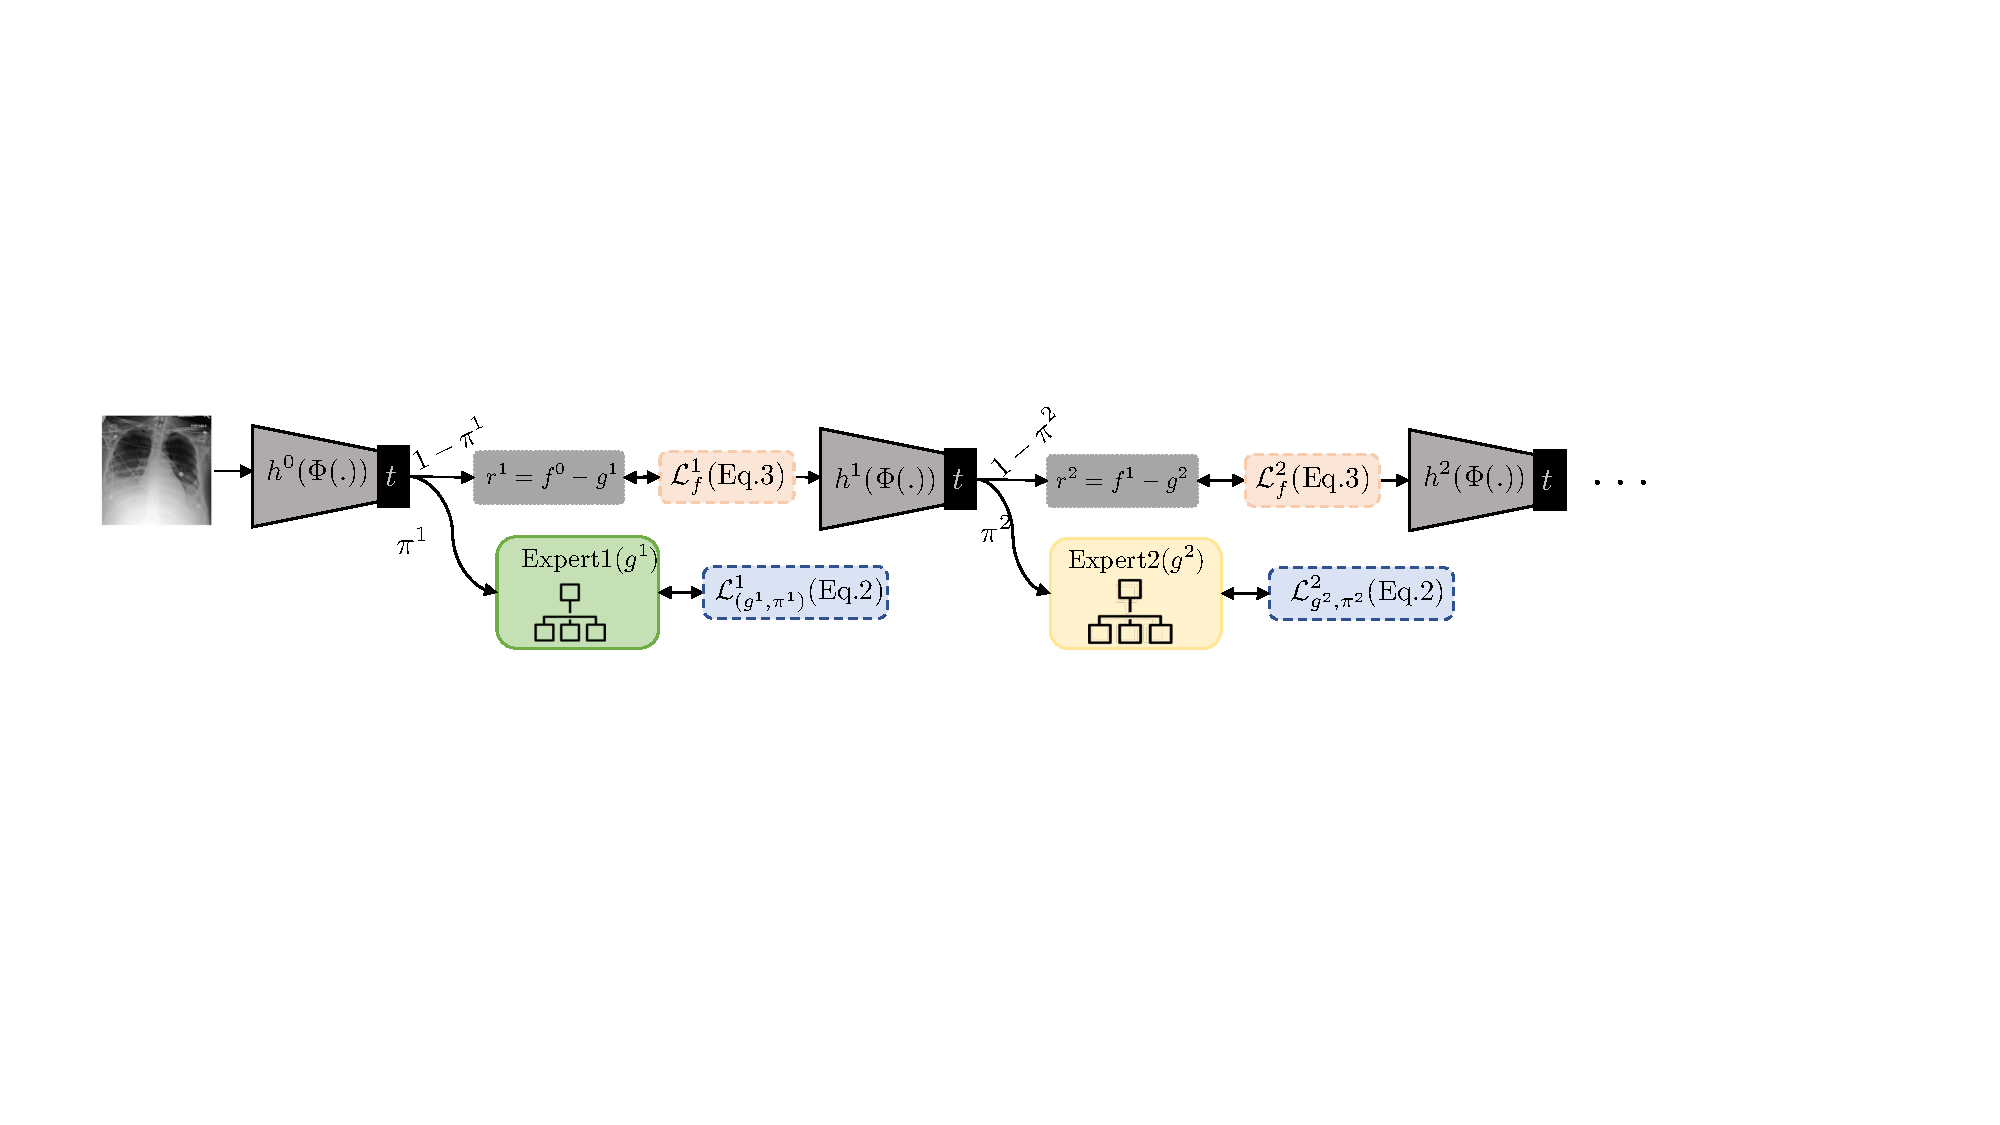
\includegraphics[width=\columnwidth]{figures/main/Schematic.pdf}}
\caption{Schematic view of \emph{route, interpret} and \emph{repeat}. At iteration $k$, the selector \emph{routes} each sample either towards the interpretable model $g^k$ (to \emph{interpret}) with probability $\pi^k(.)$ or the residual $r^k = f^{k-1} - g^k$ with probability $1-\pi^k(.)$ (to 
\emph{repeat} in the further iterations). 
$f^{k-1}$ is the Blackbox of the $(k-1)^{th}$ iteration. $g^k$ generates FOL-based explanations for the samples it covers. 
Otherwise, the selector routes through the next step until it either goes through a subsequent interpretable model or reaches the last residual. 
Components in black and grey indicate the fixed and trainable modules in our model, respectively.
}
\label{fig:Schematic} 
\end{center}
\vskip -0.2in
\end{figure}

\subsection{Neuro-Symbolic Knowledge Distillation}
Knowledge distillation in our method involves 3 parts: (1) a series of trainable selectors, \emph{routing} each sample through the interpretable models and the residual networks, (2) a sequence of learnable neuro-symbolic interpretable models, each providing FOL explanations to \emph {interpret} the Blackbox, and (3) \emph{repeating} with Residuals for the samples that cannot be explained with their interpretable counterparts. 
We detail each component below.

\subsubsection{The selector function}
As the first step of our method, the selector $\pi^k$ \emph{routes} the $j^{th}$ sample through the interpretable model $g^k$ or residual $r^k$ with probability $\displaystyle \pi^k(\boldsymbol{c_j})$ and $\displaystyle 1 - \pi^k(\boldsymbol{c_j})$ respectively, where $k$ $\in [0,K]$, with $K$ being the number of iterations.
We define the empirical coverage of the $\displaystyle k^{th}$ iteration as $\vspace{-0.08pt} \zeta(\pi^k) = \frac{1}{m}\sum_{j = 1} ^ m \pi^k(\boldsymbol{c_j}) \vspace{-0.081pt}$, the empirical mean of the samples selected by the selector for the associated interpretable model $\displaystyle g^k$, with $\displaystyle m$ being the total number of samples in the training set. Thus, the entire selective risk is:

% \vskip -7.5pt
\begin{equation}
\label{equ: emp_risk}
\mathcal{R}^k(\displaystyle \pi^k, \displaystyle g^k) = \frac{\frac{1}{m}\sum_{j=1}^m\mathcal{L}_{(g^k, \pi^k)}^k\big(\boldsymbol{x_j}, \boldsymbol{c_j}\big)}{\zeta(\pi^k)} ,
\end{equation}
% \vskip 2pt

where $\mathcal{L}_{(g^k, \pi^k)}^k$ is the optimization loss used to learn $\displaystyle g^k$ and $\displaystyle \pi^k$ together, discussed in~\cref{ns-optimization}. For a given coverage of $\displaystyle \tau^k \in (0, 1]$, we solve the following optimization problem:

\vskip -7.5pt
\begin{align}
\label{equ: optimization_g}
\theta_{s^k}^*, \theta_{g^k}^* = & \operatorname*{arg\,min}_{\theta_{s^k}, \theta_{g^k}} \mathcal{R}^k\Big(\pi^k(.; \theta_{s^k}), \displaystyle g^k(.; \theta_{g^k}) \Big) \nonumber \\ 
&\text{s.t.} ~~~ \zeta\big(\pi^k(.; \theta_{s^k})\big) \geq \tau^k,
\end{align}
\vskip 2pt

where $\theta_{s^k}^*, \theta_{g^k}^*$ are the optimal parameters at iteration $k$ for the selector $\pi^k$ and the interpretable model $g^k$ respectively. In this work, $\pi$s' of different iterations are neural networks with sigmoid activation. At inference time, the selector routes the $j^{th}$ sample with concept vector $\boldsymbol{c_j}$ to $\displaystyle g^k$ if and only if $\pi^k(\boldsymbol{c}_j)\geq 0.5$ for $k \in [0,K]$.



\subsubsection{Neuro-Symbolic interpretable models}
\label{ns-optimization}
In this stage, we design interpretable model $\displaystyle g^k$ of $k^{th}$ iteration  to \emph{interpret} the Blackbox $\displaystyle f^{k - 1}$ from the previous $(k-1)^{th}$ iteration by optimizing the following loss function:
\begin{equation}
\label{equ: g_k}
\resizebox{0.47\textwidth}{!}{$
\mathcal{L}_{(g^k, \pi^k)}^k\big(\boldsymbol{x_j}, \boldsymbol{c_j}\big) = \underbrace{\mystrut{2.6ex}\ell\Big(f^{k - 1}(\boldsymbol{x_j}), g^k(\boldsymbol{c_j})\Big)\pi^k(c_j) }_{\substack{\text{trainable component} \\ \text{for current iteration $k$}}}\underbrace{\prod_{i=1} ^{k - 1}\big(1 - \pi^i(\boldsymbol{c_j})\big)}_{\substack{\text{fixed component trained} \\ \text{in the previous iterations}}},
$}
\end{equation}

where the term $\pi^k(\boldsymbol{c_j})\prod_{i=1} ^{k - 1}\big(1 - \pi^i(\boldsymbol{c_j}) \big)$ denotes the probability of $j^{th}$ sample being routed through the interpretable model $g^k$. It is the probability of the sample going through the residuals for all the previous iterations from $1$ through $k-1$ (\ie $\prod_{i=1} ^{k - 1}\big(1 - \pi^i(\boldsymbol{c_j}) \big)$\big) times the probability of going through the interpretable model at iteration $k$ \big(\ie $\pi^k(\boldsymbol{c_j})$\big). 
Refer to~\cref{fig:Schematic} for an illustration. We learn $\pi^1, \dots \pi^{k - 1}$ in the prior iterations and are not trainable at iteration $k$. As each interpretable model $g^k$ specializes in explaining a specific subset of samples (denoted by coverage $\tau$), we refer to it as an \emph{expert}. We use SelectiveNet's ~\cite{geifman2019selectivenet}  optimization method to optimize~\cref{equ: optimization_g} since selectors need a rejection mechanism to route samples through residuals.~\cref{app:loss} details the optimization procedure in~\cref{equ: g_k}. We refer to the interpretable experts of all the iterations as a ``Mixture of Interpretable Experts'' (MoIE) cumulatively after training. Furthermore, we utilize E-LEN, \ie a Logic Explainable Network~\cite{ciravegna2023logic} implemented with an Entropy Layer as first layer~\cite{barbiero2022entropy} as the interpretable symbolic model $g$ to construct First Order Logic (FOL) explanations of a given prediction.

\subsubsection{The Residuals}
The last step is to \emph{repeat} with the residual $r^k$, as $\displaystyle r^k(\boldsymbol{x_j},\boldsymbol{c_j}) = f^{k - 1}(\boldsymbol{x_j}) - g^k(\boldsymbol{c_j})$.
We train $f^k = h^k\big(\Phi(.)\big)$ to approximate the residual $r^k$, creating a new Blackbox $f^k$ for the next iteration $(k+1$). This step is necessary to specialize $\displaystyle f^k$ over samples not covered by $g^k$. Optimizing the following loss function yields $\displaystyle f^k$ for the $\displaystyle k^{th}$ iteration:
\begin{equation}
\label{equ: residual}
\mathcal{L}_f^k(\boldsymbol{x_j}, \boldsymbol{c_j}) = \underbrace{\mystrut{2.6ex}\ell\big(r^k(\boldsymbol{x_j}, \boldsymbol{c_j}), f^k(\boldsymbol{x_j})\big)}_{\substack{\text{trainable component} \\ \text{for iteration $k$}}} \underbrace{\mystrut{2.6ex}\prod_{i=1} ^{k}\big(1 - \pi^i(\boldsymbol{c_j})\big)}_{\substack{\text{non-trainable component} \\ \text{for iteration $k$}}} 
\end{equation}

% \underbrace{\mystrut{2.6ex}\ell\big(f^{k - 1}(\boldsymbol{x_j}), g^k(\boldsymbol{c_j})\big)\pi^k(c_j) }_{\substack{\text{trainable component} \\ \text{from current iteration}}}
Notice that we fix the embedding $\displaystyle \Phi(.)$ for all the iterations. Due to computational overhead, we only finetune the last few layers of the Blackbox ($h^k$) to train $f^k$.
At the final iteration $K$, our method produces a MoIE and a Residual, explaining the interpretable and uninterpretable components of the initial Blackbox $f^0$, respectively.~\cref{app:algo} describes the training procedure of our model, the extraction of FOL, and the architecture of our model at inference.


\textbf{Selecting number of iterations $K$:} We follow two principles to select the number of iterations $K$ as a stopping criterion: 1) Each expert should have enough data to be trained reliably (
coverage $\zeta^k$). If an expert covers insufficient samples, we stop the process. 2) If the final residual ($r^K$) underperforms a threshold, it is not reliable to distill from the Blackbox. We stop the procedure to ensure that overall accuracy is maintained.

\begin{table}[t]
\caption{Datasets and Blackboxes.}
\fontsize{5.2pt}{0.30cm}\selectfont
\label{tab:dataset}
\vskip 0.1in
\begin{center}
% \begin{small}
% \begin{sc}
\begin{tabular}{lcc}
\toprule
DATASET & BLACKBOX & \# EXPERTS  \\
\midrule
CUB-200~\cite{wah2011caltech}  & RESNET101~\cite{he2016deep}& 6 \\
CUB-200~\cite{wah2011caltech}  & VIT~\cite{wang2021feature}&  6 \\
AWA2~\cite{xian2018zero} & RESNET101~\cite{he2016deep} & 4\\
AWA2~\cite{xian2018zero} & VIT~\cite{wang2021feature} & 6\\
HAM1000~\cite{tschandl2018ham10000}    & INCEPTION~\cite{szegedy2015going}& 6\\
SIIM-ISIC~\cite{rotemberg2021patient}    & INCEPTION~\cite{szegedy2015going} & 6\\
EFFUSION IN MIMIC-CXR~\cite{12_johnsonmimic}    & DENSENET121~\cite{huang2017densely} & 3\\
\bottomrule
\end{tabular}
% \end{sc}
% \end{small}
\end{center}
\vskip -0.1in
\end{table}

\begin{figure*}[t]
\vskip 0.1in
\begin{center}
\centerline{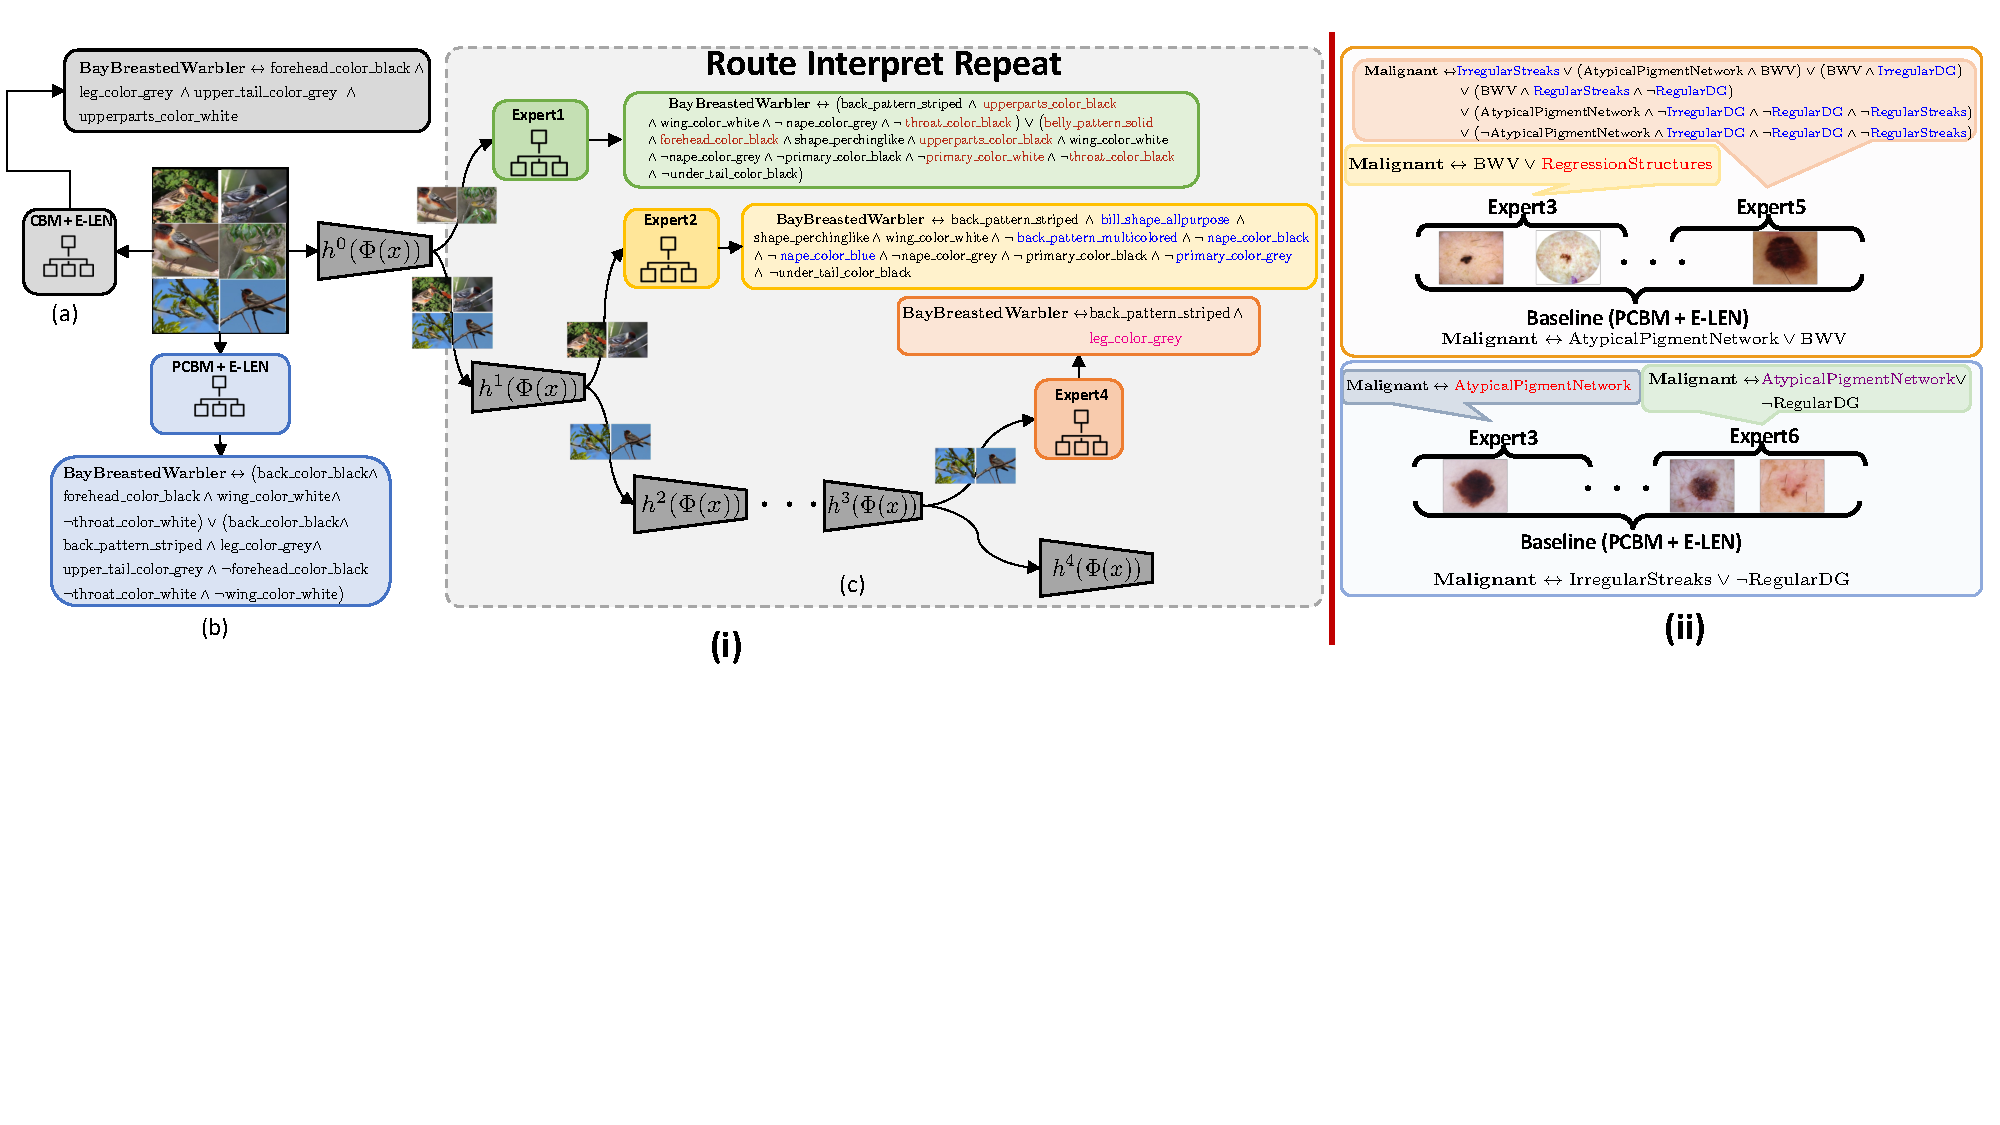
\includegraphics[width=\linewidth]{figures/main/Results_all.pdf}}
\caption{MoIE identifies diverse concepts for specific subsets of a class, unlike the generic ones by the baselines. \textbf{(i)} We construct the FOL explanations of the samples of, ``Bay breasted warbler'' in the CUB-200 dataset for VIT-based \textbf{(a)} CBM + E-LEN as an \emph{interpretable-by-design} baseline, \textbf{(b)} PCBM + E-LEN as a \emph{posthoc} baseline, \textbf{(c)} experts in MoIE at inference. We highlight the unique concepts for experts 1,2, and 3 in~\emph{red},~\emph{blue}, and~\emph{magenta}, respectively. \textbf{(ii)} Comparison of FOL explanations by MoIE with the PCBM + E-LEN baselines for HAM10000 (\textbf{top}) and ISIC (\textbf{down})  to classify Malignant lesion. We highlight unique concepts for experts 3, 5, and 6 in \emph{red}, \emph{blue}, and \emph{violet}, respectively. For brevity, we combine the local FOLs for each expert for the samples covered by them, shown in the figure.}
\label{fig:local_ex_cub}
\end{center}
\vskip -0.1in
\end{figure*}

\section{Related work}
%% Post hoc methods
% Saliency cam grad cam
% attribution lime shap l2x

% interpretable models
% early GAM - tabular data
% CBM no composability
% E-LENS FOL

\textbf{Post hoc explanations:} 
Related work in Post-hoc explanation techniques include: 1) highlighting relevant pixels in the image~\cite{simonyan2013deep, selvaraju2017grad, smilkov2017smoothgrad, sundararajan2017axiomatic, binder2016layer}, 2) developing a surrogate linear function~\cite{ribeiro2016should, yoon2019rl} to imitate the Blackbox around a local neighborhood, and 3) using the game-theoretic SHAPLY values~\cite{SHAP} to determine feature importance in the Blacbox prediction. Though post hoc explanations retain the flexibility and performance of the Blackbox, they operate in pixel space, often not corresponding to humanly interpretable \emph{concepts}~\cite{kim2017interpretability}. This restricts the use of post-hoc methods in algorithmic recourse~\cite{bordt2022post}. In this paper, we offer a post hoc explanation of the Blackbox in terms of concepts to improve interpretability and facilitate test-time interventions on the concepts.

\textbf{Concept-based interpretable models:}
Concept-based interpretable models leverage the weak annotations of visual attributes to predict the concepts from images and then the class labels from the concepts, as in Concept Bottleneck models (CBMs)~\cite{koh2020concept}. A concept decoder is used in the antehoc model~\cite{sarkar2021inducing} to simultaneously reconstruct the image from the concepts to ensure the semantics of the input image from the concepts, specifically aiming for unsupervised concept discovery. Instead of learning scalar concepts in the bottleneck, end-to-end Concept Embedding models (CEMs)~\cite{zarlenga2022concept} uses high dimensional concept embeddings to allow extra supervised learning capacity and achieves SOTA performance in the interpretable-by-design class. An inherently interpretable ELL~\cite{barbiero2022entropy} introduces an entropy-based classifier for the downstream classification and provides explanations in terms of FOL using the concepts. Recently, Posthoc Concept Bottleneck models (PCBMs) ~\cite{yuksekgonul2022post} learn the concepts from a trained Blackbox  embeddings and uses an interpretable classifier for classification. Also, they fit a residual in their hybrid variant (PCBM-h) to mimic the performance of the Blackbox. However, all these methods employ a single interpretable model to explain a Blackbox. Thus, they offer generic explanations for all the samples of a class, lowering the performance, particularly for models that are inherently interpretable. Also PCBMs do not provide any reasoning through the identified concepts. Our MoIE overcomes these issues by 1) employing multiple experts to carve instance-specific concepts from the Blackbox while preserving its flexibility and performance, 2) providing fundamental reasoning on concepts by offering FOL explanations per sample, 3) fitting residuals in each iteration to progressively cover samples in an increasing order of ``hardness''.

\textbf{Shortcut learning:}
Often, a Blackbox leverages spurious correlations, having no semantic connection to the actual task. These spurious correlations are termed as ``shortcuts''.  that the model exploits for its decision without any connection to the actual task. Related work in explainability includes LIME~\cite{ribeiro2016should}, utilized to detect spurious background as a shortcut to classify an animal. Recently interpretable model~\cite{rosenzweig2021patch}, involving local image pathces, are used as a proxy to the Blackbox to identify shortcuts. However, both of them function in pixel space, notconcept space. Also, they do not eliminate the shortcut.  Our MoIE discovers shortcuts using the high level concepts in the FOL explanation of the Blackbox's prediction and eliminates them via Meta data normalization (MDN)~\cite{lu2021metadata}.

\textbf{Post hoc explanations:} 
Post hoc explanations retain the flexibility and performance of the Blackbox. The post hoc explanation has many categories, including feature attribution~\cite{simonyan2013deep, smilkov2017smoothgrad, binder2016layer} and counterfactual approaches~\cite{singla2019explanation, abid2021meaningfully}. For example, feature attribution methods associate a measure of importance to features (e.g., pixels) that is proportional to the feature's contribution to BlackBox's predicted output. Many methods were proposed to estimate the importance measure, including gradient-based methods~\cite{selvaraju2017grad, sundararajan2017axiomatic}, game-theoretic approach~\cite{SHAP}. The post hoc approaches suffer from a lack of fidelity to input~\cite{adebayo2018sanity} and ambiguity in explanation due to a lack of correspondence to human-understandable concepts. Recently, Posthoc Concept Bottleneck models (PCBMs) ~\cite{yuksekgonul2022post} learn the concepts from a trained Blackbox embedding and use an interpretable classifier for classification. Also, they fit a residual in their hybrid variant (PCBM-h) to mimic the performance of the Blackbox. We will compare against the performance of the PCBMs method. Another major shortcoming is that, due to a lack of mechanistic explanation, post hoc explanations do not provide a recourse when an undesirable property of a Blackbox is identified. Interpretable-by-design provides a remedy to those issues~\cite{rudin2019stop}.




\textbf{Concept-based interpretable models:}
Our approach falls into the category of concept-based interpretable models. 
% Our approach falls into the category of interpretable-by-design.
Such methods provide a mechanistically interpretable prediction that is a function of human-understandable concepts. The concepts are usually extracted from the activation of the middle layers of the Neural Network (bottleneck). Examples include Concept Bottleneck models (CBMs)~\cite{koh2020concept},  antehoc concept decoder~\cite{sarkar2021inducing}, and a high-dimensional Concept Embedding model (CEMs)~\cite{zarlenga2022concept} that uses high dimensional concept embeddings to allow extra supervised learning capacity and achieves SOTA performance in the interpretable-by-design class. Most concept-based interpretable models do not model the interaction between concepts and cannot be used for reasoning. An exception is E-LEN~\cite{barbiero2022entropy} which uses an entropy-based approach to derive explanations in terms of FOL using the concepts. The underlying assumption of those methods is that one interpretable function can explain the entire set of data, which can limit flexibility and consequently hurt the performance of the models. Our approach relaxes that assumption by allowing multiple interpretable functions and a residual. Each function is appropriate for a portion of the data, and a small portion of the data is allowed to be uninterpretable by the model (\ie residual). We will compare our method with CBMs, CEMs, and their E-LEN-enhanced variants. 
 


\textbf{Application in fixing the shortcut learning:}
Shortcuts are spurious features that correlate with both input and the label on the training dataset but fail to generalize in more challenging real-world scenarios. Explainable AI (X-AI) aims to identify and fix such an undesirable property. Related work in X-AI includes LIME~\cite{ribeiro2016should}, utilized to detect spurious background as a shortcut to classify an animal. Recently interpretable model~\cite{rosenzweig2021patch}, involving local image patches, are used 
as a proxy to the Blackbox to identify shortcuts. However, both methods operate in pixel space, not concept space. Also, both approaches are post hoc and do not provide a way to eliminate the shortcut 
learning problem. Our MoIE discovers shortcuts using the high-level concepts in the FOL explanation of the Blackbox's prediction and eliminates them via metadata normalization (MDN)~\cite{lu2021metadata}.



\begin{figure*}[ht]
\vskip 0.2in
\begin{center}
\centerline{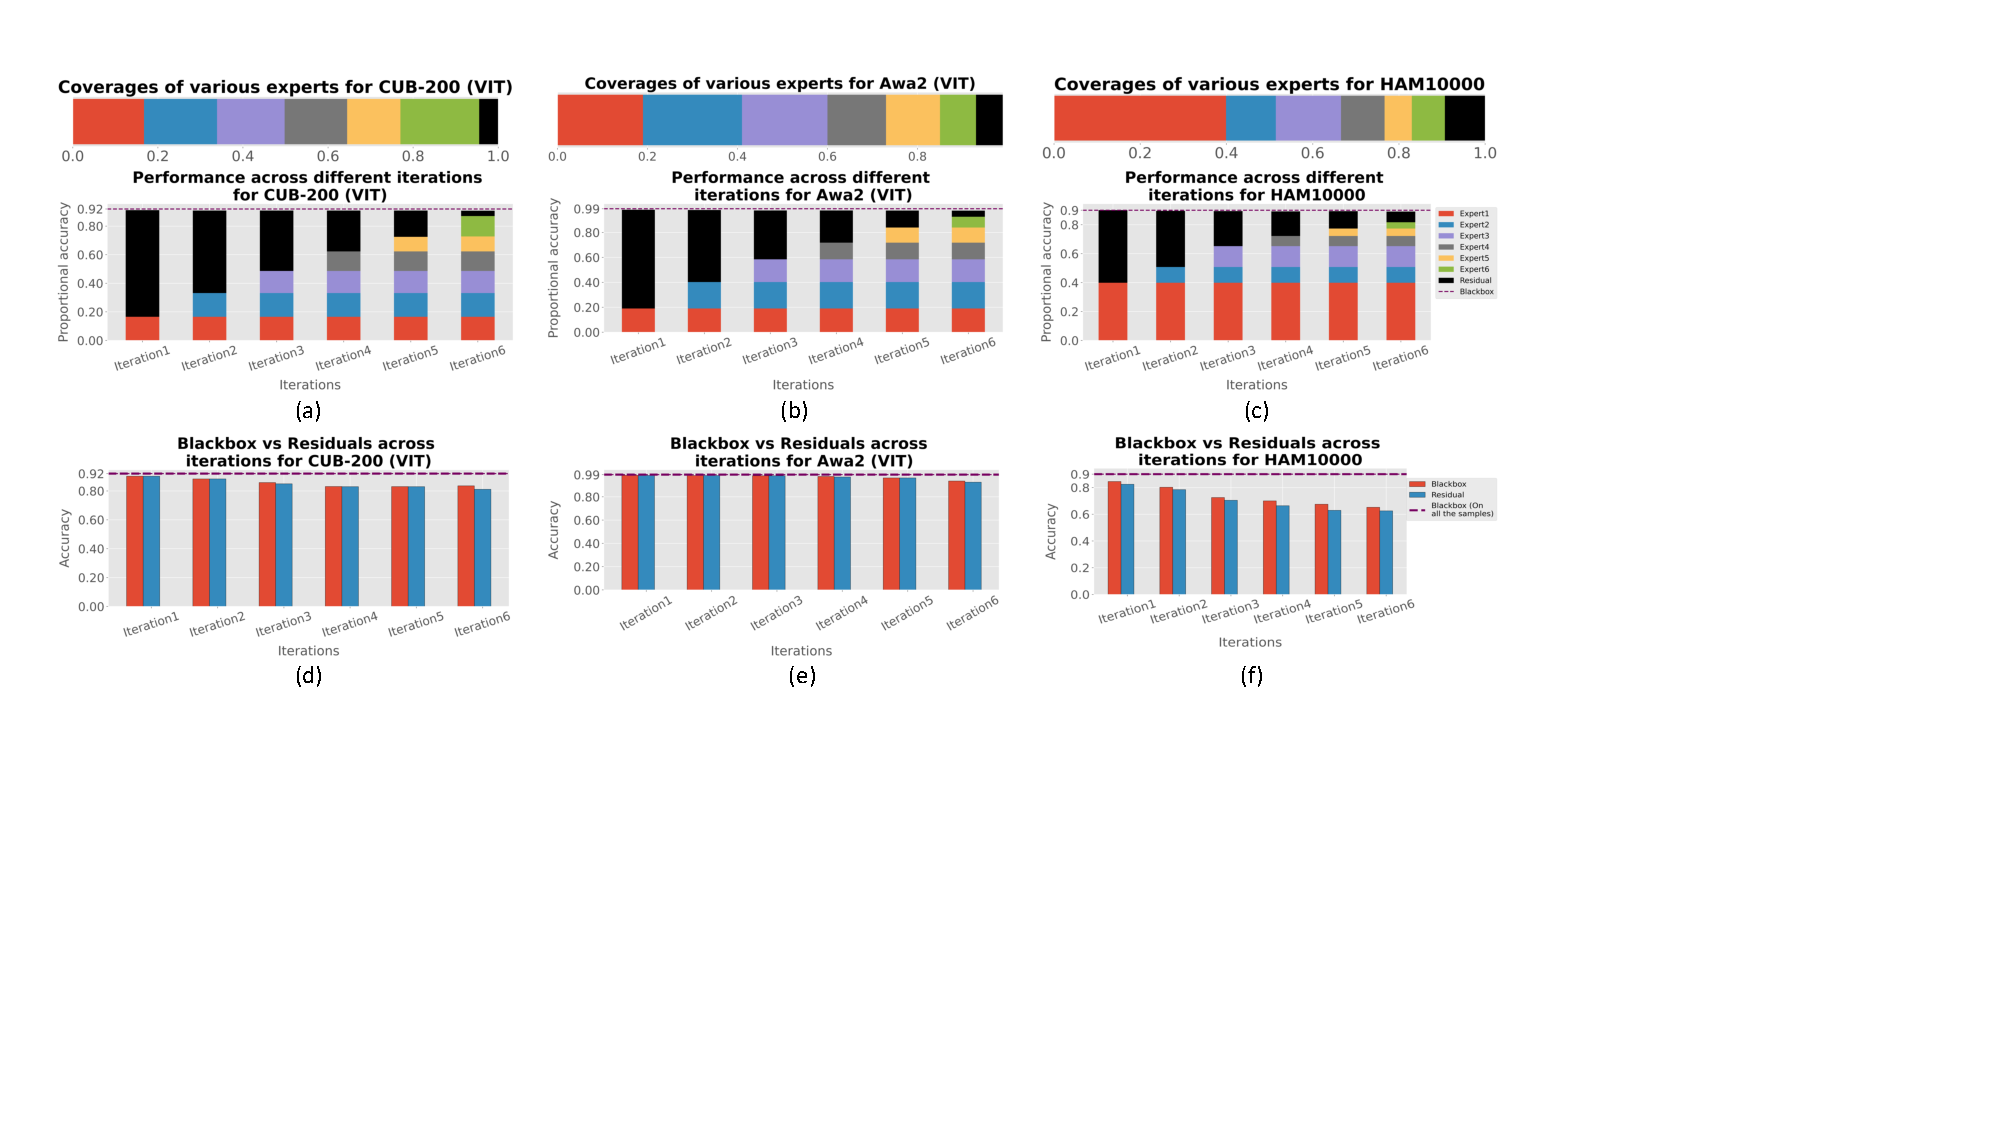
\includegraphics[width=\linewidth]{figures/main/Expert_res_all.pdf}}
\caption{The performance of experts and residuals across iterations. 
\textbf{(a-c)} Coverage and proportional accuracy of the experts and residuals. 
\textbf{(d-f)} We route the samples covered by the residuals across iterations to the initial Blackbox $f^0$ and compare the accuracy of $f^0$ (red bar) with the residual (blue bar). Figures \textbf{d-f} show the progressive decline in performance of the residuals across iterations as they cover the samples in the increasing order of ``hardness''. We observe the similar abysmal performance of the initial blackbox $f^0$ for these samples.
}
\label{fig:expert_performance_cv_vit}
\end{center}
\vskip -0.2in
\end{figure*}


\section{Experiments}

% We evaluate MoIE on five datasets - 1) bird classification using CUB-200 \cite{wah2011caltech} dataset, 2) animal classification using Animals with Attributes2 (Awa2) dataset \cite{xian2018zero}, 3) skin lesion classification using the HAM10000 dataset \cite{tschandl2018ham10000}, 4) . 5) classification of the disease Effusion using the MIMIC-CXR dataset \cite{12_johnsonmimic}. 
We perform experiments on a variety of vision and medical imaging datasets to show that 1) MoIE captures a diverse set of concepts, 2) the performance of the residuals degrades over successive iterations as they cover ``harder'' instances, 3) MoIE does not compromise the performance of the Blackbox, 4) MoIE achieves superior performances during test time interventions, and 5) MoIE can fix the shortcuts using the Waterbirds dataset \cite{sagawa2019dro}. We repeat our method until MoIE covers at least 90\% of samples or the final residual's accuracy falls below 70\%. Furthermore, we only include concepts as
input to $g$ if their validation accuracy or auroc exceeds a certain threshold (in all of our experiments,
we fix 0.7 or 70\% as the threshold of validation auroc or accuracy). Refer to~\cref{tab:dataset} for the datasets and Blackboxes experimented with. For convolution based Blackboxes (ResNets, Densenet121 and Inception), we flatten the feature maps from the last convolutional block to extract the concepts. For VITs, we use the image embeddings from the transformer encoder to perform the same. We use SIIM-ISIC as a real-world transfer learning setting, with the Blackbox trained on HAM10000 and evaluated on a subset of the SIIM-ISIC Melanoma Classification dataset~\cite{yuksekgonul2022post}.~\cref{app:dataset} and~\cref{app:g} expand on the datasets and hyperparameters.
% \textbf{Training configurations:} CUB-200 and Awa2 use ResNet101~\cite{he2016deep} and Vision Transformer (VIT)~\cite{wang2021feature} as blackboxes. HAM10000 and MIMIC-CXR use Inception~\cite{szegedy2015going} and Densenet121~\cite{huang2017densely}, respectively. For CUB-200, we use 6 experts each for both VIT and ResNet-based Blackboxes. For Awa2, we utilize 4 and 6 experts for ResNet-101 and VIT, respectively. For skin lesion classification (both HAM10000 and SIIM-ISIC) and MIMIC-CXR, we use 6 and 3 experts, respectively. Appendices~\ref{app:dataset} and~\ref{app:g} detail the datasets and hyperparameters.

\begin{figure*}[ht]
\vskip 0.2in
\begin{center}
\centerline{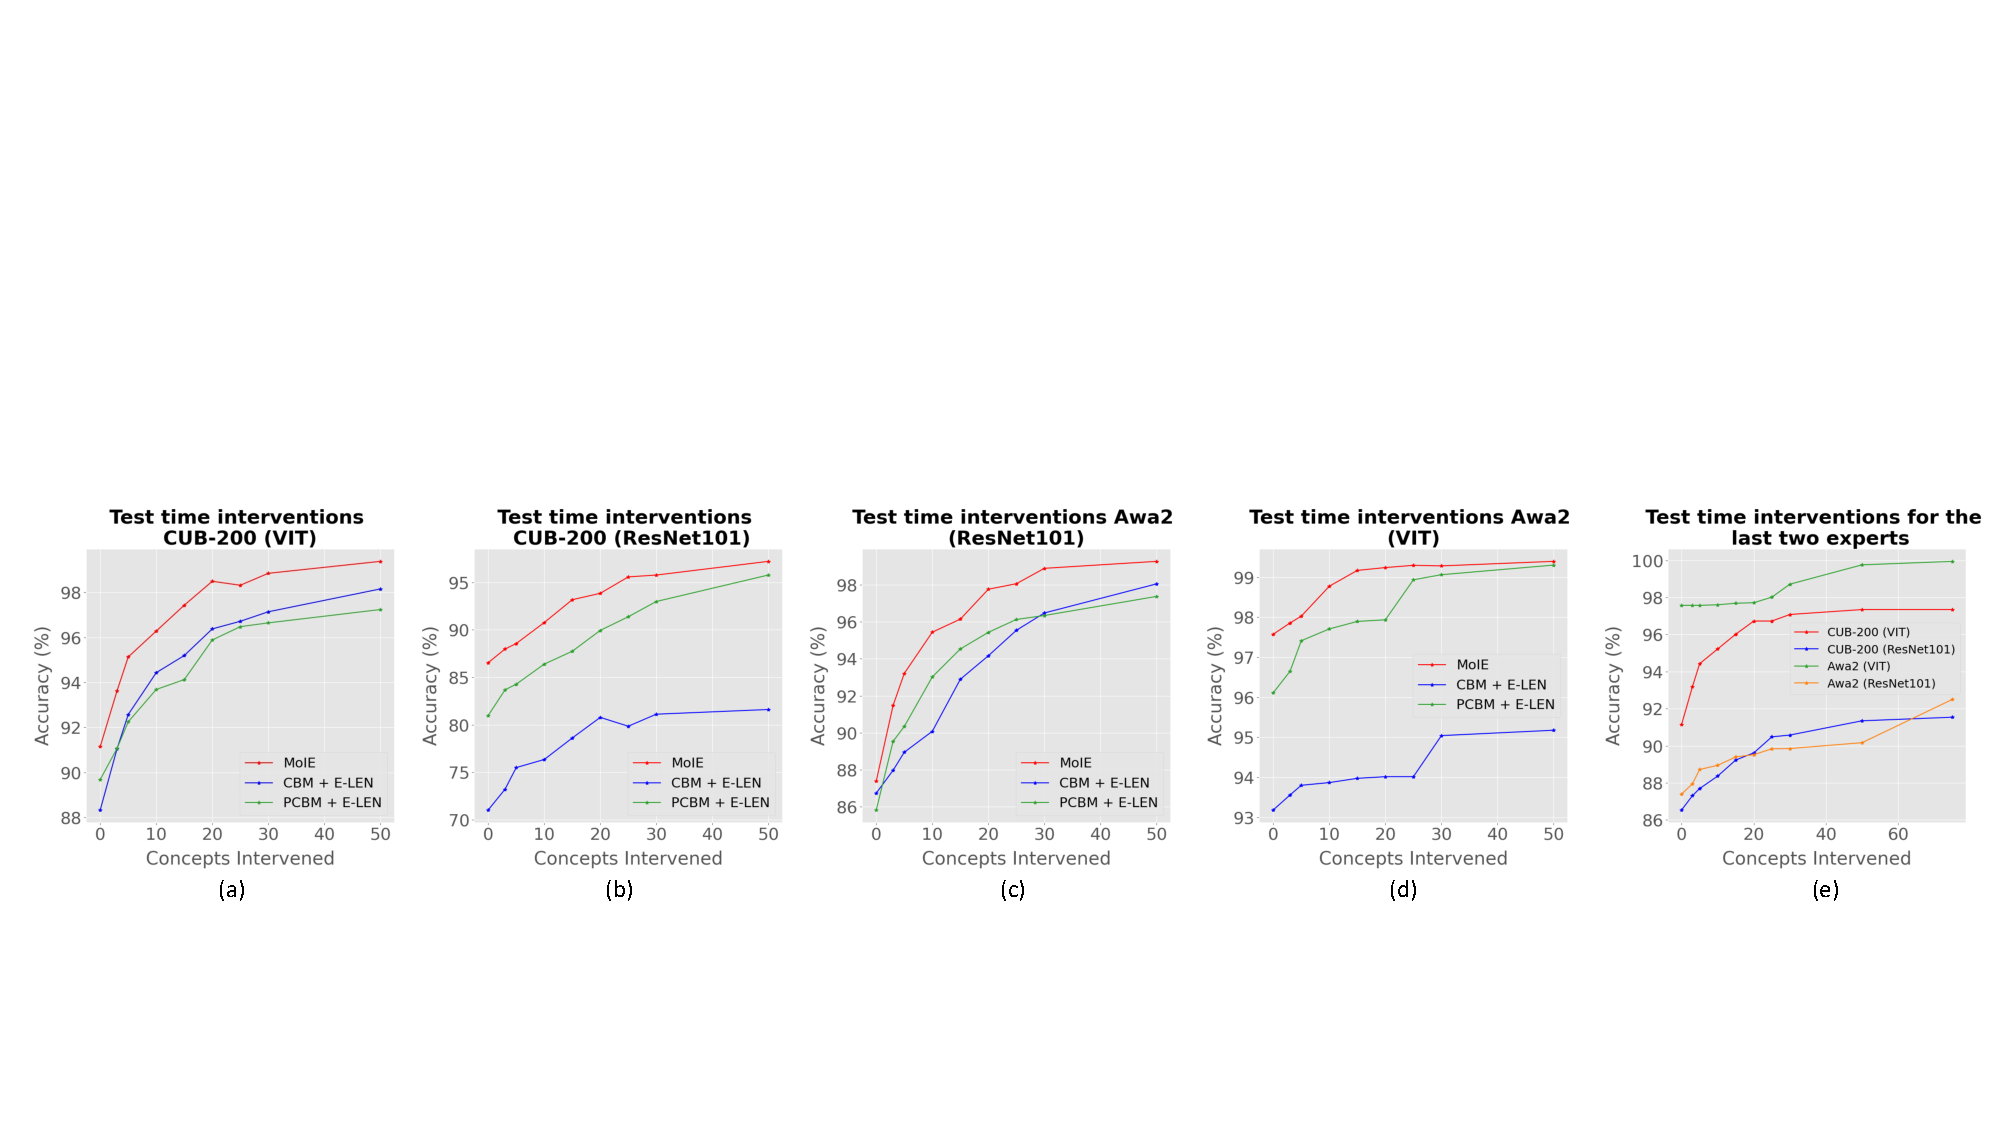
\includegraphics[width=\linewidth]{figures/main/TTI_all.pdf}}
\caption{Across architectures test time interventions of concepts  on all the samples \textbf{(a-d)}, on the ``hard'' samples \textbf{(e)}, covered by only the last two experts of MoIE. 
% All the plots mark the first point on the x-axis as "0," indicating the original model's performance with no intervention
}
\label{fig:tti}
\end{center}
\vskip -0.2in
\end{figure*}

% \begin{figure}[h]
% % \vskip 0.1in
% \begin{center}
% \centerline{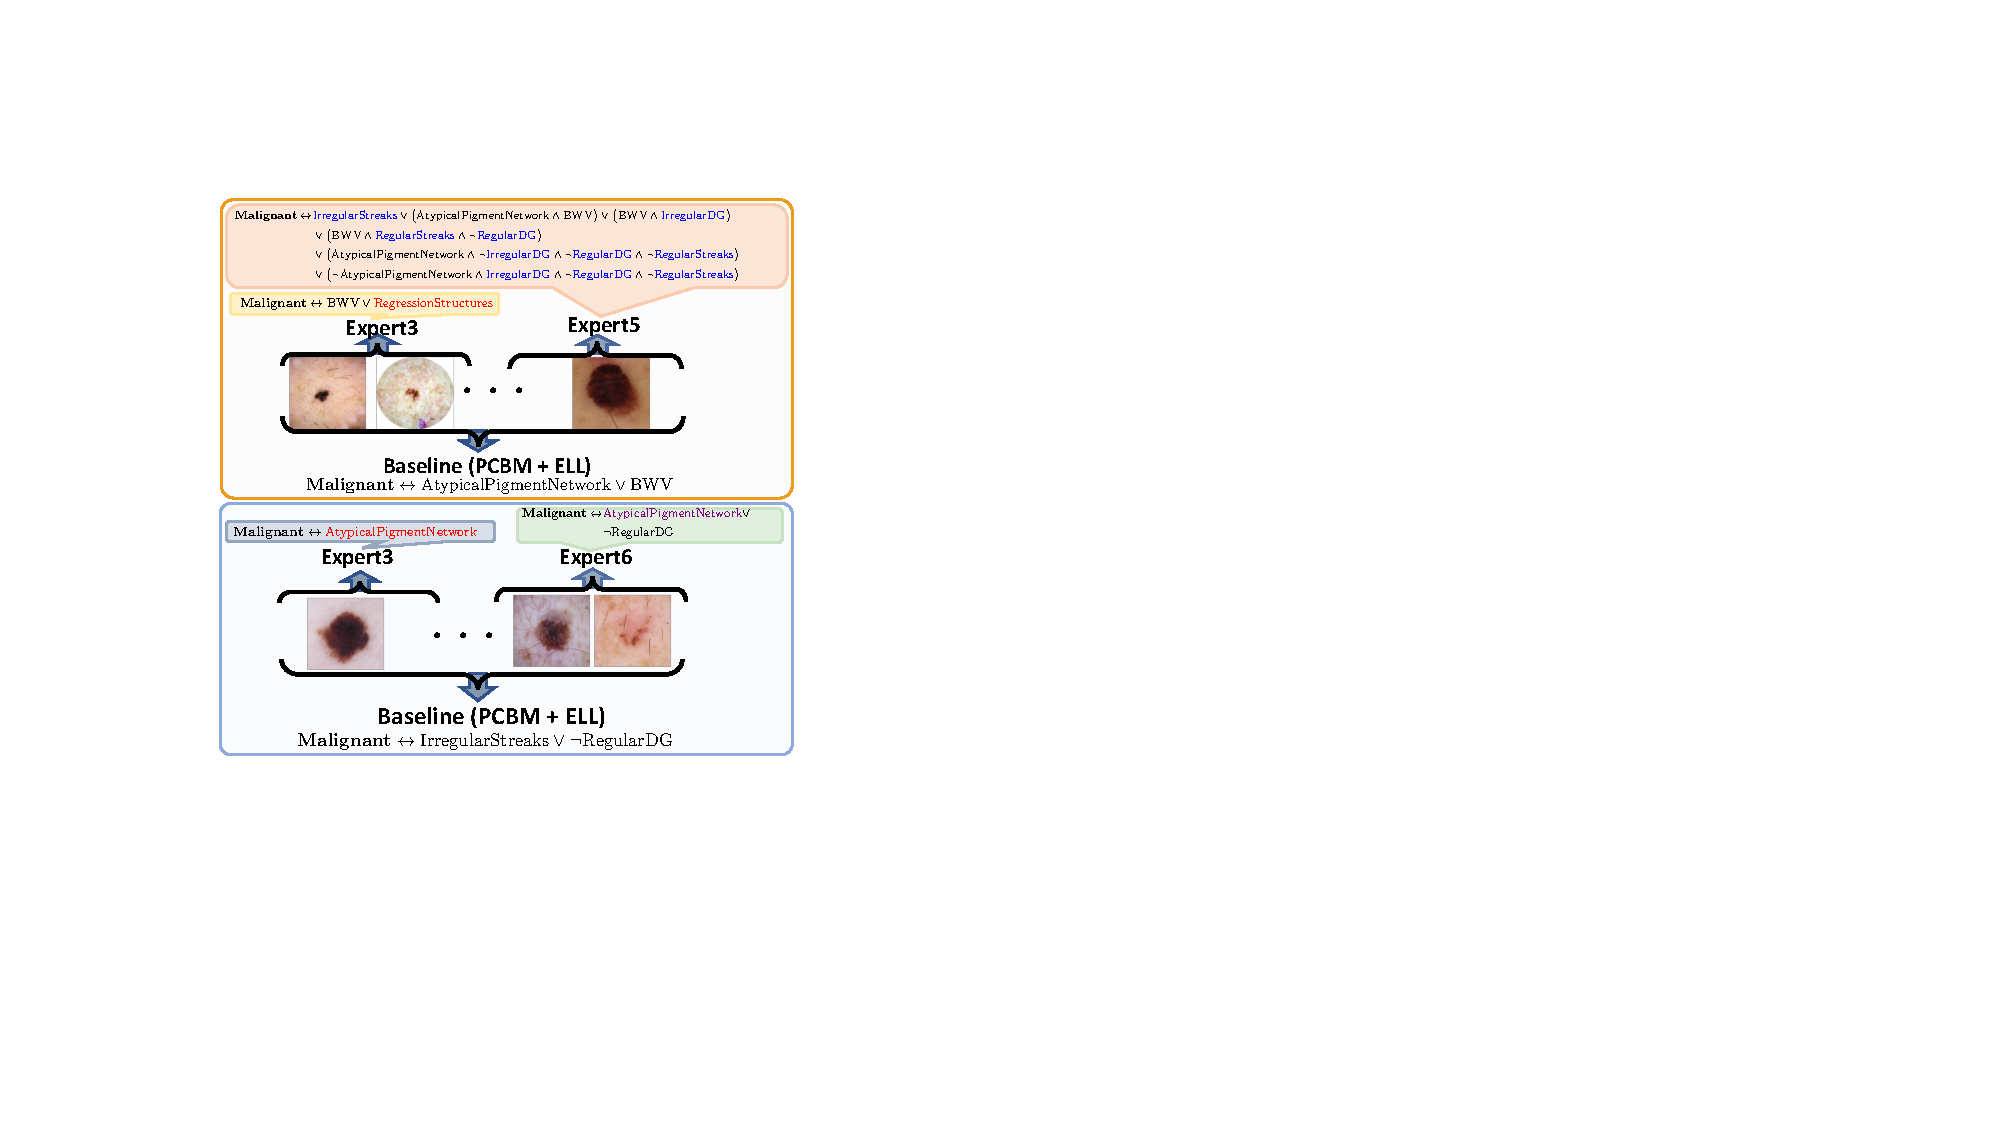
\includegraphics[width=\columnwidth]{figures/main/Local.pdf}}
% \caption{Flexibility of FOL explanations by MoIE compared to the PCBM + E-LEN baselines for HAM10000 (\emph{top}) and ISIC (\emph{down})  to classify Malignant lesion. We highlight unique concepts for experts 3, 5 and 6 in \emph{red}, \emph{blue} and \emph{violet} respectively.}
% \label{fig:local_awa2_skin}
% \end{center}
% \vskip -0.23in
% \end{figure}

\begin{figure}[h]
% \vskip 0.1in
\begin{center}
\centerline{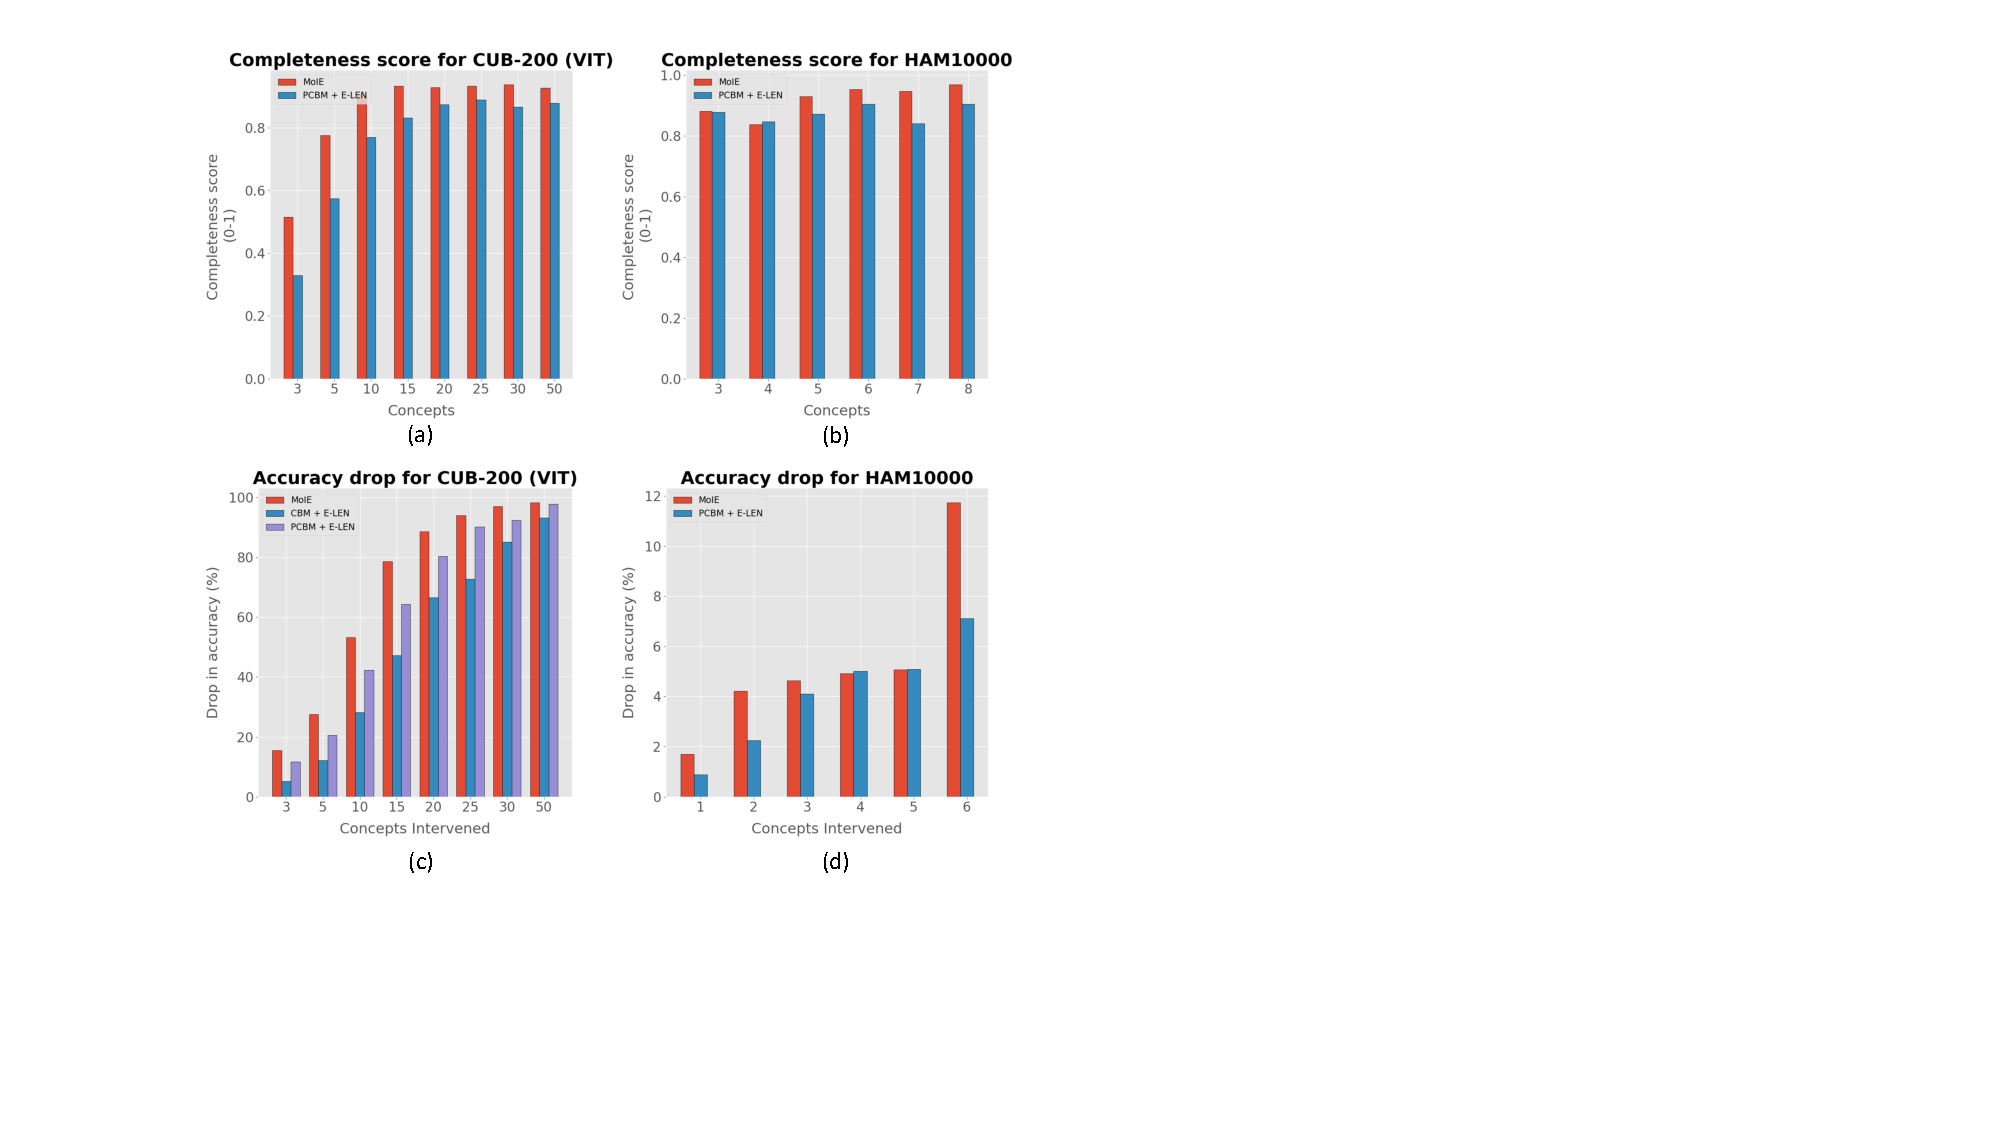
\includegraphics[width=\columnwidth]{figures/main/CUB_HAM.pdf}}
\caption{Quantitative validation of the extracted concepts. \textbf{(a-b)} 
Completeness scores of the models for a varying number of top concepts. (\textbf{c-d)} Drop in accuracy compared to the original model after zeroing out the top significant concepts iteratively. The highest drop for MoIE indicates that MoIE selects more instance-specific concepts than generic ones by the baselines. 
% All the plots mark the first point on the x-axis as "0," indicating the original model's performance with no intervention
}
\label{fig:valid_concepts}
\end{center}
\vskip -0.2in
\end{figure}


\textbf{Baselines:}
We compare our methods to two concept-based baselines -- 1) interpretable-by-design and 2) posthoc. They consist of two parts: a) a concept predictor $\Phi: \mathcal{X} \rightarrow \mathcal{C}$, predicting concepts from images; and b) a label predictor $g: \mathcal{C} \rightarrow \mathcal{Y}$, predicting labels from the concepts. The end-to-end CEMs and sequential CBMs serve as interpretable-by-design baselines. Similarly, PCBM and PCBM-h serve as post hoc baselines. Convolution-based $\Phi$ includes all layers till the last convolution block. VIT-based $\Phi$ consists of the transformer encoder block. The standard CBM and PCBM models do not show how the concepts are composed to make the label prediction. So, we create CBM + E-LEN, PCBM + E-LEN and PCBM-h + E-LEN by using the identical $g$ of MOIE (shown in~\cref{app:g}), as a replacement for the standard classifiers of CBM and 
PCBM. We train the $\Phi$ and $g$ in these new baselines to sequentially generate FOLs~\cite{barbiero2022entropy}. Due to the unavailability of concept annotations, we extract the concepts from the Derm7pt dataset~\cite{kawahara2018seven} using the pre-trained embeddings of the Blackbox~\cite{yuksekgonul2022post} for HAM10000. Thus, we do not have interpretable-by-design baselines for HAM10000 and ISIC.



\subsection{Results}
% \subsection{Baseline}
% \label{app:baseline}
% We compare our methods to two baselines -- 1) interpretable by design 2) posthoc concept bottlenecks (PCBMs). For interpretable by design, we employ the end to end concept embedding models (CEMs)~\cite{zarlenga2022concept} and sequential concept bottleneck models (CBMs)~\cite{koh2020concept}, consisting of two parts: 1) a concept extractor $\phi: \mathcal{X} \rightarrow \mathcal{C}$, predicting concepts from images; and 2) a classifier $g: \mathcal{C} \rightarrow \mathcal{Y}$, predicting labels from the concepts. Convolution-based $\phi$ includes all layers till the last convolution block. VIT-based $\phi$ consists of the transformer encoder block (excluding the classification head). For PCBMs, we employ the similar strategy described in~\cite{yuksekgonul2022post} to classify using the extracted the concepts from image embeddings of a trained blackbox. Furthermore, we use the identical $g$ of MOIE (as in Appendix \ref{app:g}) replacing the label predictors of CBM and PCBM to compare our FOL explanations with the baselines. Henceforth, we refer them as CBM + ELL and PCBM + ELL. As~\cite{barbiero2022entropy} trains the concept and label predictors sequentially, we also perform the same for the CBM + ELL and PCBM + ELL baselines. For HAM10000 dataset, we extract the concepts from Derm7pt dataset using the pretrained embeddings of the blackbox as per~\cite{yuksekgonul2022post}. Thus, we can not use interpretable by design baselines for HAM10000 and SIIM-ISIC due to the unavailability of concept annotations in the dataset.

\subsubsection{Expert driven explanations by MoIE }
% Our paper aims at constructing a mixture of experts specializing in a subset of the test set to provide local explanations. Due to space constraints, we report the analysis of the HAM10000 and CUB datasets in this section. Appendices \ref{app:awa2_resutls} and \ref{app:mimic_cxr_resutls} include the resutls of Awa2 and MIMIC-CXR datasets, respectively. 
% As shown in E-Lens~\cite{barbiero2022entropy}, each expert constructs local FOL per sample, composing the concepts based on their attention weights. 

First, we show that MoIE captures a rich set of diverse instance-specific concepts qualitatively. Next, we show quantitatively that MoIE-identified concepts are faithful to Blackbox's final prediction using the metric ``completeness score'' and zeroing out relevant concepts.


\textbf{Heterogenity of Explanations:}
At each iteration of MoIE, the blackbox \big($h^k(\Phi(.)$\big) splits into an interpretable expert ($g^k$) and a residual ($r^k$).~\cref{fig:local_ex_cub}i shows this mechanism for VIT-based MoIE and compares the FOLs with CBM + E-LEN and PCBM + E-LEN baselines to classify ``Bay Breasted Warbler'' of CUB-200.
The experts of different iterations specialize in specific instances of ``Bay Breasted Warbler''. Thus, each expert's FOL comprises its instance-specific concepts of the same class. For example, the concept, \emph{leg\_color\_grey} is unique to expert4, but \emph{belly\_pattern\_solid} and \emph{back\_pattern\_multicolored} are unique to experts 1 and 2, respectively, to classify the instances of ``Bay Breasted Warbler'' in the ~\cref{fig:local_ex_cub}(i)-c. 
% Also, FOLs from all three experts share \emph{back\_pattern\_stripped}. 
Unlike MoIE, the baselines employ a single interpretable model $g$, resulting in a generic FOL with identical concepts for all the samples of ``Bay Breasted Warbler'' (\cref{fig:local_ex_cub}i(a-b)). Thus the baselines fail to capture the heterogeneity of explanations. Due to space constraint, we combine the local FOLs of different samples. For additional results of CUB-200, refer to~\cref{app:local_cub}.
% Appendix \ref{app:more_cub_results} display more instances of such global explanations.

\cref{fig:local_ex_cub}ii shows such diverse local instance-specific explanations for HAM10000 (\emph{top}) and ISIC (\emph{bottom}). In~\cref{fig:local_ex_cub}ii-(top), the baseline-FOL consists of concepts such as \emph{AtypicalPigmentNetwork} and \emph{BlueWhitishVeil (BWV)} to classify ``Malignancy'' for all the instances for HAM10000. However, expert~3 relies on \emph{RegressionStructures} along with \emph{BWV} to classify the same for the samples it covers while expert~5 utilizes several other concepts \eg \emph{IrregularStreaks}, \emph{Irregular dots and globules (IrregularDG)} \etc \text{ }Due to space constraints,~\cref{app:local_awa2} reports similar results for the Awa2 dataset. Also, VIT-based experts compose less concepts per sample than the ResNet-based experts, shown in~\cref{app:comparison_arch}.

\begin{table*}[t]
\caption{MoIE does not hurt the performance of the original Blackbox using a held-out test set. We 
provide the mean and standard errors of AUROC and accuracy for medical imaging (\eg HAM10000, ISIC, and Effusion) and vision (\eg CUB-200 and Awa2) datasets, respectively, over 5 random seeds. For MoIE, we also report the percentage of test set samples covered by all experts as ``coverage''. Here, MoIE + Residual represents the experts with the final residual. Following the setting~\cite{zarlenga2022concept}, we only report the performance of the convolutional CEM, leaving the construction of VIT-based CEM as a future work. Recall that interpretable-by-design models can not be constructed for HAM10000 and ISIC as they have no concept annotation; we learn the concepts from the Derm7pt dataset. For all the datasets, MoIE covers a significant portion of data (at least 90\%) cumulatively. We boldface our results. 
}
\fontsize{5pt}{0.20cm}\selectfont
\label{tab:performance}
% \vskip 0.15in
\begin{center}
% \begin{small}
% \begin{sc}
\begin{tabular}{p{25.5em} p{7.5em} p{7.5em} p{7.5em} p{7.5em} p{7.5em} p{7.5em} p{7.5em}}
\toprule 
        \textbf{MODEL} & \multicolumn{7}{c}{\textbf{DATASET}} \\
       & CUB-200 (RESNET101) & CUB-200 (VIT) & AWA2 (RESNET101) & AWA2 (VIT) & HAM10000 & SIIM-ISIC & EFFUSION  \\
\midrule 
    BLACKBOX & 0.88 & 0.92 & 0.89 & 0.99 & 0.96 & 0.85 & 0.91\\
\midrule
    \textbf{INTERPRETABLE-BY-DESIGN} \\
    CEM~\cite{zarlenga2022concept} & 0.77 $\pm$ 0.22 & - & 0.88 $\pm$ 0.50 & - & NA & NA & 0.76 $\pm$ 0.00\\
    CBM (Sequential)~\cite{koh2020concept} & 0.65 $\pm$ 0.37 & 0.86 $\pm$ 0.24 & 0.88 $\pm$ 0.35 & 0.94 $\pm$ 0.28  & NA & NA  
    & 0.79 $\pm$ 0.00 \\ 
    CBM + E-LEN~\cite{koh2020concept, barbiero2022entropy} & 0.71 $\pm$ 0.35 & 0.88 $\pm$ 0.24 & 0.86 $\pm$ 0.35 & 0.93 $\pm$ 0.25 & NA & NA & 
    0.79 $\pm$ 0.00  \\
\midrule
     \textbf{POSTHOC} \\
     PCBM~\cite{yuksekgonul2022post} & 0.76 $\pm$ 0.01  & 0.85 $\pm$ 0.20 & 0.82 $\pm$ 0.23 & 0.94 $\pm$ 0.17 &
     0.93 $\pm$	0.00 & 0.71 $\pm$	0.01 & 0.81 $\pm$	0.01\\
     PCBM-h~\cite{yuksekgonul2022post} & 0.85 $\pm$ 0.01  & 0.91 $\pm$ 0.18 & 0.87 $\pm$ 0.20 & 0.98 $\pm$ 0.17 &
     0.95 $\pm$	0.00 & 0.79 $\pm$	0.05 & 0.87 $\pm$	0.07\\
     PCBM + E-LEN~\cite{yuksekgonul2022post, barbiero2022entropy} &  0.80 $\pm$ 0.36 & 0.89 $\pm$ 0.26 & 0.85 $\pm$ 0.25 & 0.96 $\pm$ 0.18 & 
     0.94 $\pm$	0.02 &  0.73 $\pm$	0.01 & 0.81 $\pm$	0.01\\
     PCBM-h + E-LEN~\cite{yuksekgonul2022post, barbiero2022entropy} &  0.85 $\pm$ 0.30 & 0.91 $\pm$ 0.28 & 0.88 $\pm$ 0.24 & 0.98 $\pm$ 0.20 & 
     0.95 $\pm$	0.03 &  0.82 $\pm$	0.05 & 0.87 $\pm$	0.03\\
\midrule
     \textbf{OURS} \\
     MoIE (COVERAGE) &\textbf{0.86 $\pm$ 0.01 (0.9)} &\textbf{0.91 $\pm$ 0.00 (0.95)} &
     \textbf{0.87 $\pm$ 0.02 (0.91)} & \textbf{0.97 $\pm$ 0.00 (0.94)} & \textbf{0.95 $\pm$	0.00 (0.9)}
     & \textbf{0.84 $\pm$ 0.00 (0.94)} & \textbf{0.87 $\pm$	0.00 (0.98)}\\
     MoIE + RESIDUAL & \textbf{0.84 $\pm$ 0.01} & \textbf{0.90 $\pm$ 0.01} & \textbf{0.86 $\pm$ 0.020} & \textbf{0.94 $\pm$ 0.004}
     & \textbf{0.92 $\pm$	0.00} & \textbf{0.82 $\pm$	0.01} & \textbf{0.86 $\pm$	0.00} \\
\bottomrule
\end{tabular}
% \end{sc}
% \end{small}
\end{center}
% \vskip -0.1in
\end{table*}

\textbf{MoIE-identified concepts attain higher completeness scores.} 
\cref{fig:valid_concepts}(a-b) shows the completeness scores~\cite{yeh2019concept} for varying number of concepts.
 Completeness score is a post hoc measure, signifying the identified concepts as ``sufficient statistic'' of the predictive capability of the Blackbox. Recall that $g$ utilizes E-LEN~\cite{barbiero2022entropy}, associating each concept with an attention weight after training. A concept with high attention weight implies its high predictive significance.
 Iteratively, we select the top relevant concepts based on their attention weights and compute the completeness scores for the top concepts for MoIE and the PCBM + E-LEN baseline in \cref{fig:valid_concepts}(a-b) (~\cref{app:completeness} for details).
 For example, MoIE achieves a completeness score of 0.9 compared to 0.75 of the baseline($\sim 20\%\uparrow$) for the 10 most significant concepts for the CUB-200 dataset with VIT as Blackbox.
 
\textbf{MoIE identifies more meaningful instance-specific concepts.} 
\cref{fig:valid_concepts}(c-d) reports the drop in accuracy by zeroing out the significant concepts.
Any interpretable model ($g$) supports concept-intervention~\cite{koh2020concept}. 
After identifying the top concepts from $g$ using the attention weights, as in the last section, we set these concepts' values to zero, compute the model's accuracy drop, and plot in~\cref{fig:valid_concepts}(c-d). When zeroing out the top 10 essential concepts for VIT-based CUB-200 models, MoIE records a drop of 53\% compared to 28\% and 42\% for the CBM + E-LEN and PCBM + E-LEN baselines, respectively, showing the faithfulness of the identified concepts to the prediction.

% generic baseline
In both of the last experiments, MoIE outperforms the baselines as the baselines mark the same concepts as significant for all samples of each class. However,
MoIE leverages various experts specializing in different subsets of samples of different classes. 
% Thus, MoIE identifies more diverse instance-specific concepts, resulting in a superior completeness score and a severe drop in performance due to zeroing out the essential concepts compared to the baselines. 
For results of MIMIC-CXR and Awa2, refer to~\cref{app:mimic_cxr} and~\cref{app:awa2} respectively.





\subsubsection{Identification of harder samples by successive residuals}
\label{Sec:residual}
%  No mention of coparison of baselines
\cref{fig:expert_performance_cv_vit} (a-c) display the proportional accuracy of the experts and the residuals of our method per iteration. The proportional accuracy of each model (experts and/or residuals) is defined as the accuracy of that model times its coverage. Recall that the model's coverage is the empirical mean of the samples selected by the selector. 
% Since some experts only cover a ``Benign'' or a ``Malignant'' sample, we provide the accuracy rather than the AUROC for HAM10000 herewith because it would otherwise result in a random AUROC for that expert.
\cref{fig:expert_performance_cv_vit}a show that the experts and residual cumulatively achieve an accuracy $\sim$ 0.92 for the CUB-200 dataset in iteration 1, with more contribution from the residual (black bar) than the expert1 (blue bar). Later iterations cumulatively increase and worsen the performance of the experts and corresponding residuals, respectively. The final iteration carves out the entire interpretable portion from the Blackbox $f^0$ via all the experts, resulting in their more significant contribution to the cumulative performance. The residual of the last iteration covers the ``hardest'' samples, achieving low accuracy. Tracing these samples back to the original Blackbox $f^0$, it also classifies these samples poorly (\cref{fig:expert_performance_cv_vit}{(d-f)}).
As shown in the coverage plot, this experiment reinforces~\cref{fig:Schematic}, where the flow through the experts gradually becomes thicker compared to the narrower flow of the residual with every iteration. Refer to~\cref{fig:expert_performance_cv_resnet} in the~\cref{app:resnet_cv} for the results of the ResNet-based MoIEs.





\subsubsection{Quantitative analysis of MoIE with the blackbox and baseline}
% \begin{figure}[h]
% \centering
% 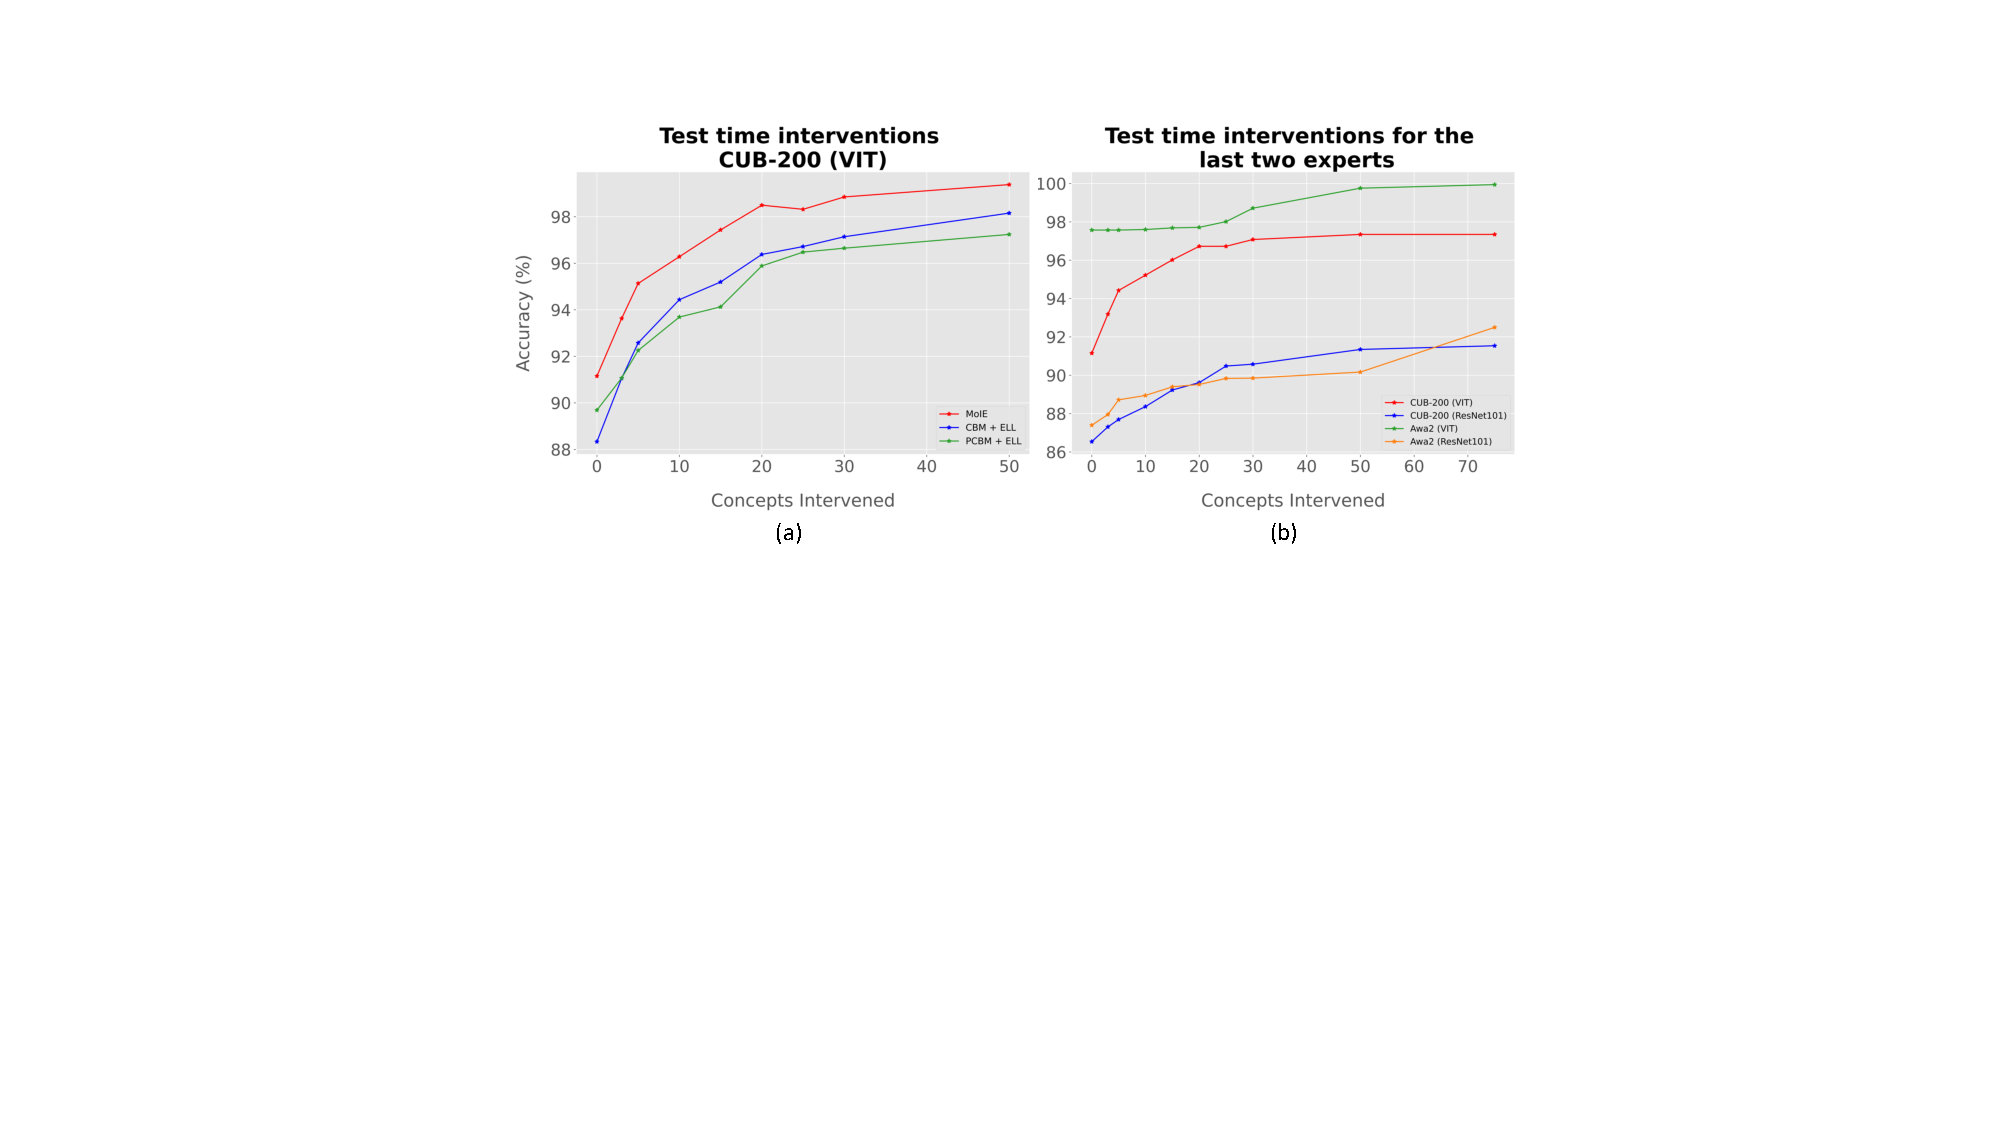
\includegraphics[width=\columnwidth]{figures/main/TTI_expert.pdf}
% \caption{Test time interventions of concepts for (a) on all the samples covered by MoIE, showing MoIE's superior performance over the baselines, (b) on the ``hard'' samples, covered by only the last two experts of MoIE across architectures. All the plots mark the first point on the x-axis as "0," indicating the original model's performance with no intervention.}
% \vskip 0.1in
% \label{fig:tti_expert}
% \end{figure}

\textbf{Comparing with the interpretable-by-design baselines:}~\cref{tab:performance} shows that MoIE achieves comparable performance to the Blackbox. Recall that ``MoIE'' refers to the mixture of all interpretable experts ($g$) only excluding any residuals.
% Also, interpretable-by-design models can not be directly constructed for HAM10000 and ISIC as they have no concept annotation~\cite{yuksekgonul2022post}.
MoIE outperforms the interpretable-by-design baselines for all the datasets except Awa2. Since Awa2 is designed for zero-shot learning, its rich concept annotation makes it appropriate for interpretable-by-design models. In general, VIT-derived MoIEs perform better than their ResNet-based variants.

\textbf{Comparing with the PCBMs:}~\cref{tab:performance} shows that interpretable MoIE outperforms the interpretable posthoc baselines -- PCBM and PCBM + E-LEN for all the datasets, especially by a significant margin for CUB-200 and ISIC.
 We also report ``MoIE + Residual'' as the mixture of interpretable experts plus the final residual to compare with the residualized PCBM, \ie PCBM-h.~\cref{tab:performance} shows that PCBM-h performs slightly better than MoIE + Residual. Note that PCBM-h learns the residual by fitting the complete dataset to fix the interpretable PCBM's mistakes to replicate the performance of the Blackbox, resulting in better performance for PCBM-h than PCBM. However, we assume the Blackbox to be a combination of interpretable and uninterpretable components. So, we train the experts and the final residual to cover the interpretable and uninterpretable portions of the Blackbox respectively. In each iteration, our method learns the residuals to focus on the samples, which are not covered by the respective interpretable experts. Therefore, residuals are not designed to fix the mistakes made by the experts. In doing so, the final residual in MoIE + Residual covers the ``hardest'' examples, lowering its overall performance compared to MoIE. 
% Note that we could not plot auroc for the other datasets that are performing multi-class 
% classification

\subsubsection{Test time interventions}
\begin{figure}
\centering
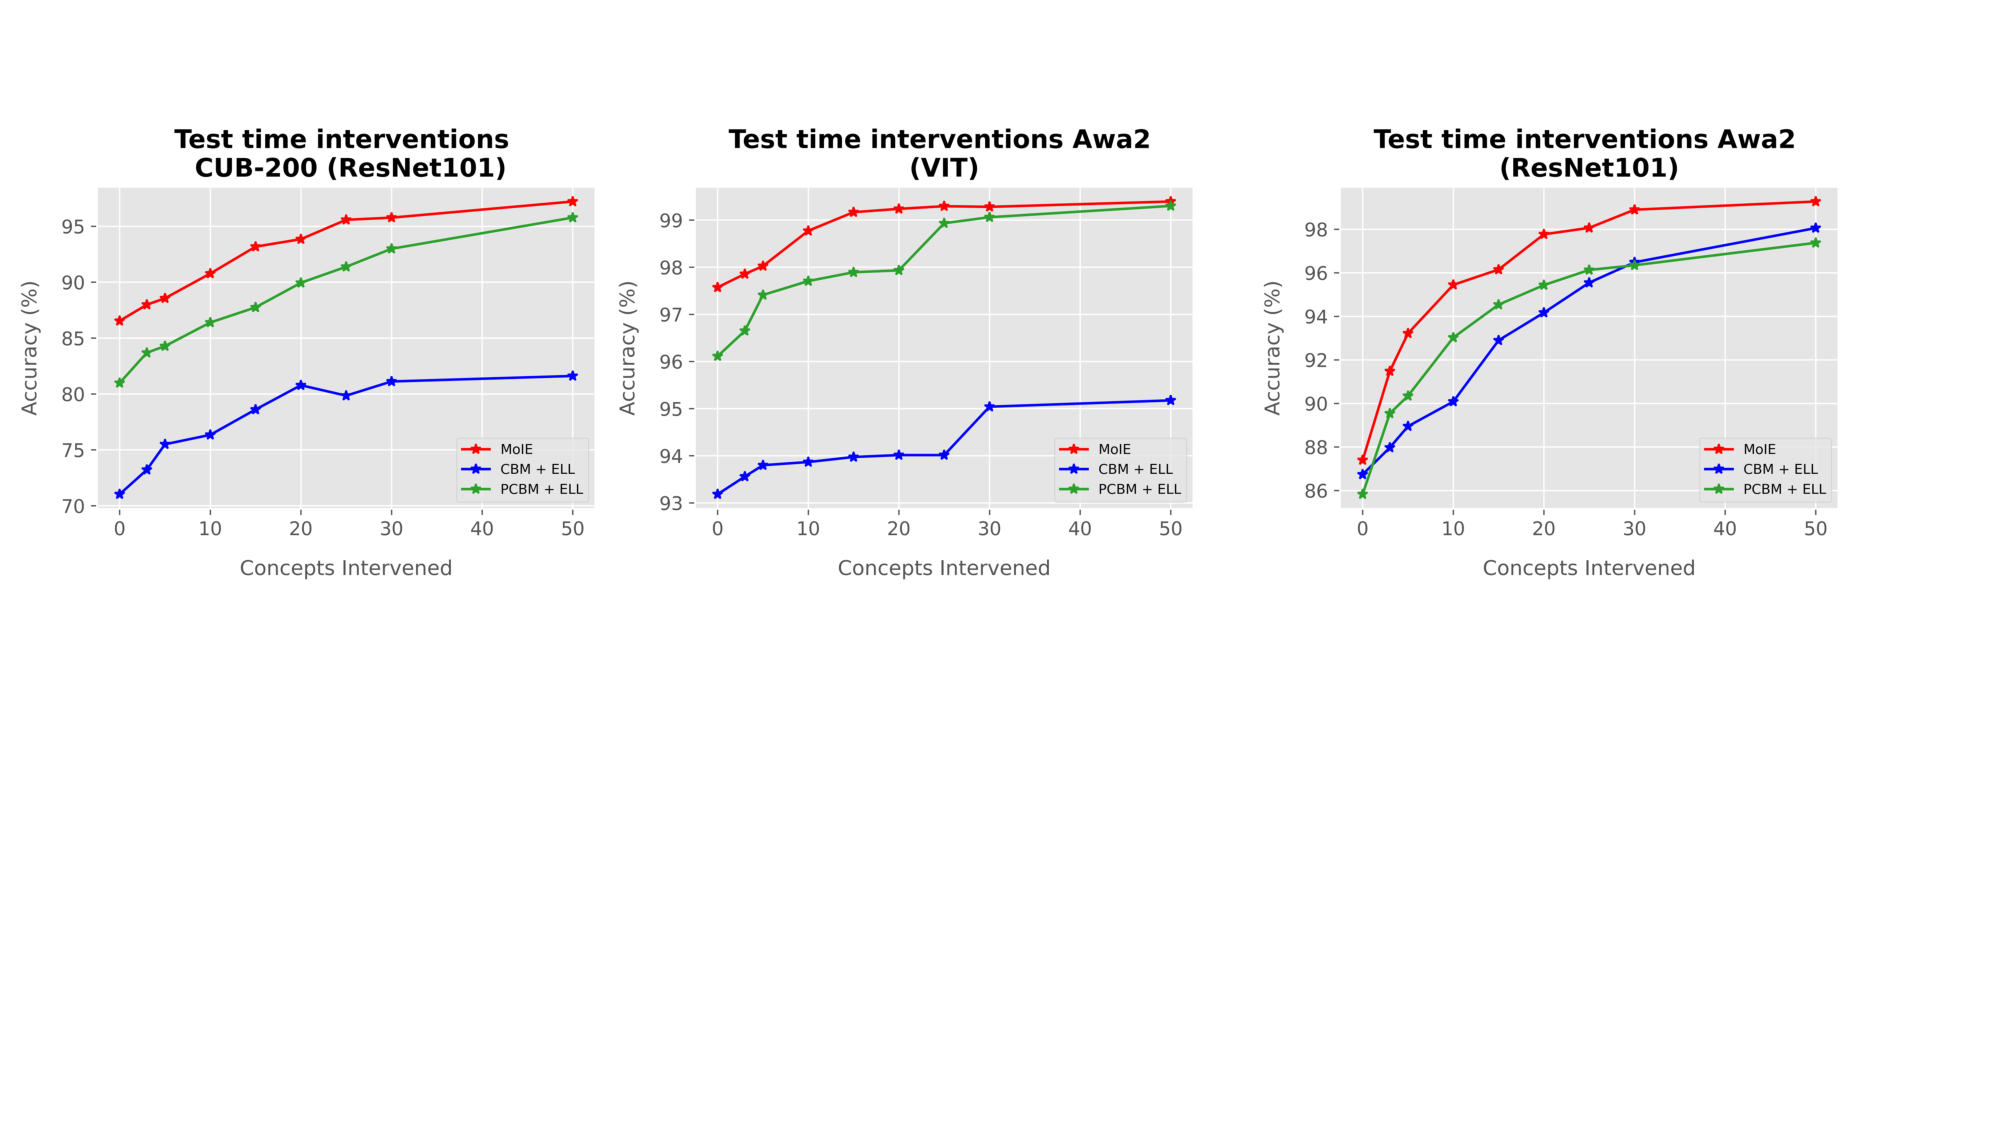
\includegraphics[width=\columnwidth]{figures/Supp/TTI_rest.pdf}
\vskip -7pt
\caption{Illustration of test time interventions for ResNet101-derived models for CUB-200 (left) and VIT-derived models for Awa2 (middle) and ResNet101-driven models for Awa2 (right).}
\vskip -7pt
\label{fig:tti_expert}
\end{figure}

Figure~\ref{fig:tti_expert} shows the results of test time concept interventions for ResNet101-derived models for CUB-200 (left) and VIT-derived models for Awa2 (middle) and ResNet101-driven models for Awa2 (right).

\subsubsection{Application in the removal of shortcuts}
\begin{figure}[ht]
% \vskip 0.2in
\begin{center}
\centerline{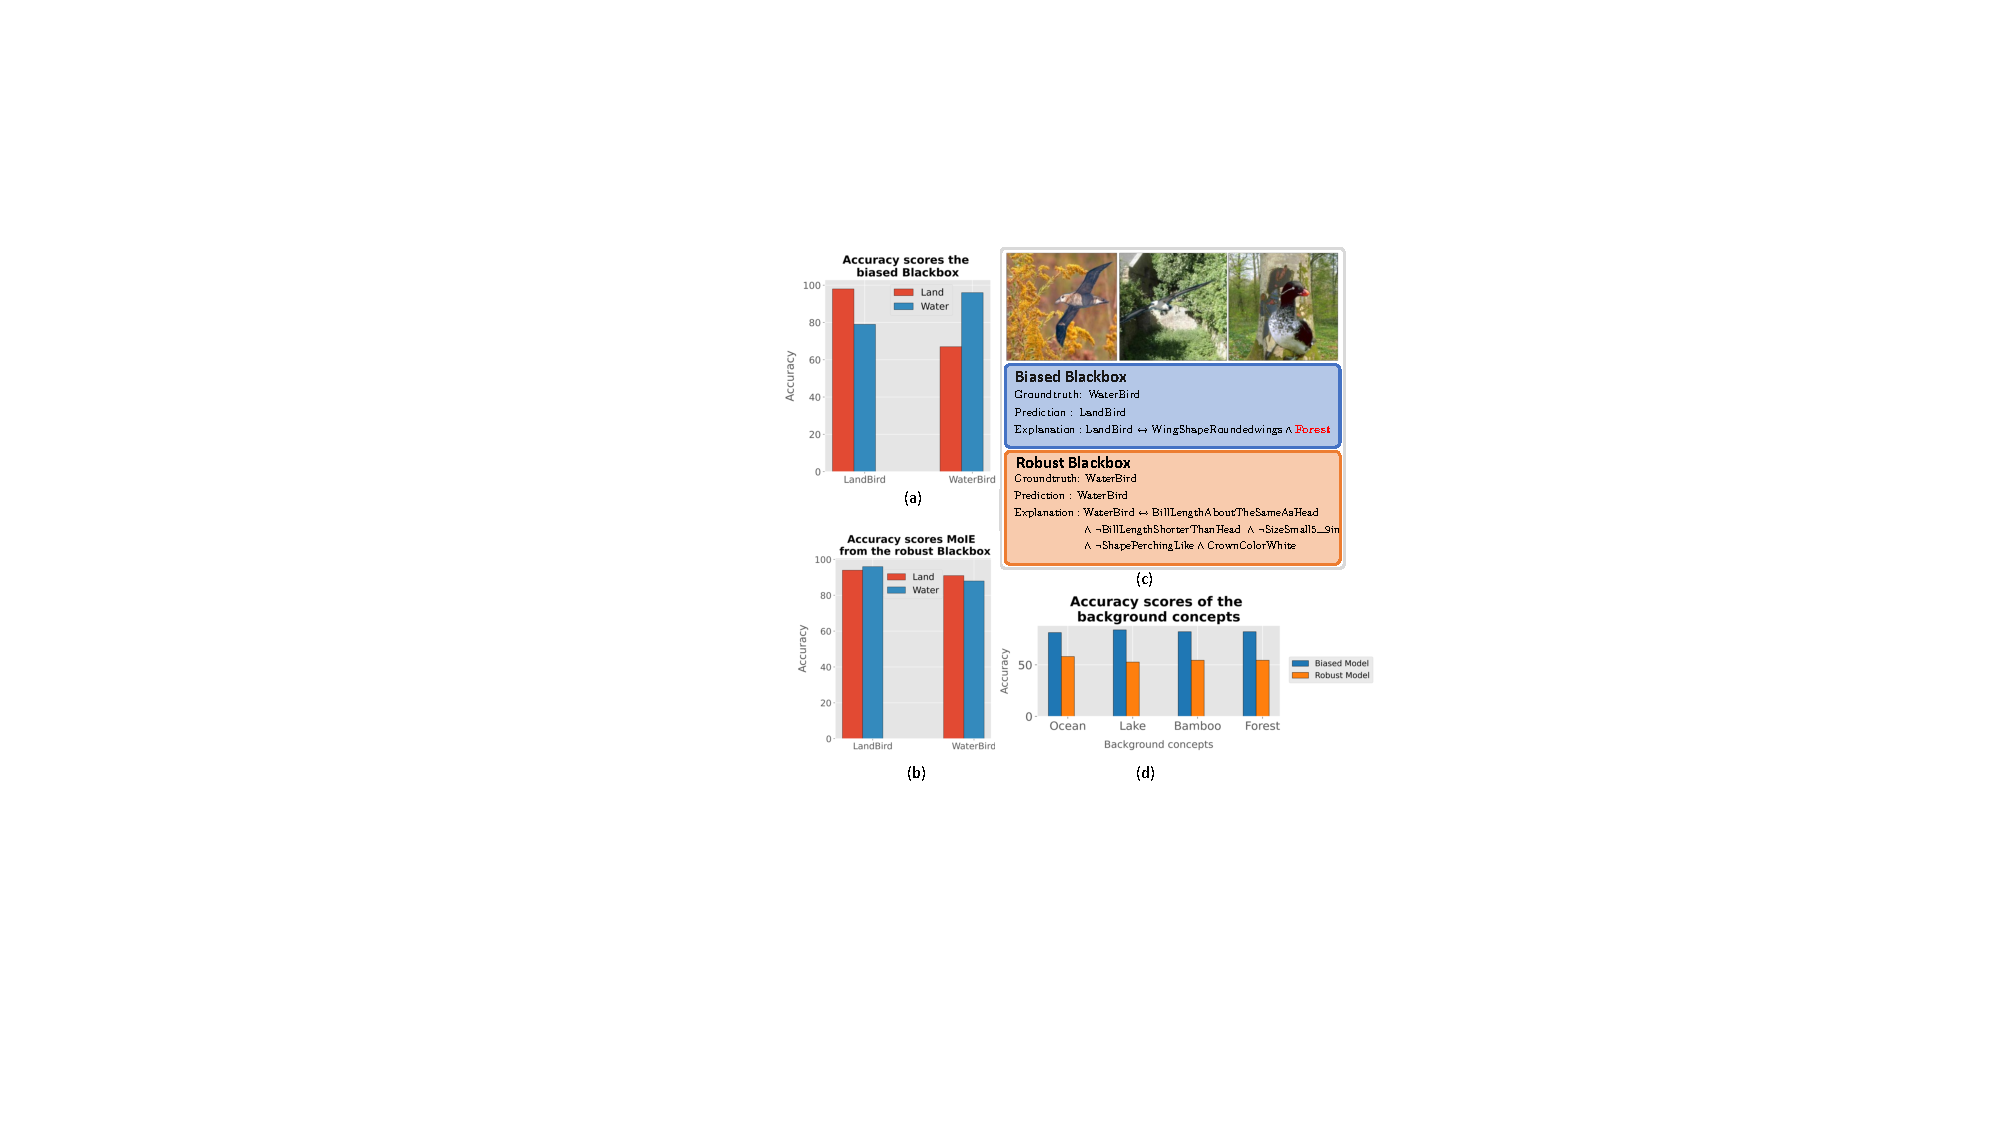
\includegraphics[width=\columnwidth]{figures/main/shortcut.pdf}}
\caption{MoIE fixes shortcuts. \textbf{(a)} Performance of the biased Blackbox. 
\textbf{(b)} Performance of final MoIE extracted from the robust Blackbox after removing the shortcuts using MDN. 
\textbf{(c)} Examples of samples (\textbf{top-row}) and their explanations by the biased (\textbf{middle-row}) and robust Blackboxes (\textbf{bottom-row}). 
\textbf{(d)} Comparison of accuracies of the spurious concepts extracted from the biased vs. the robust Blackbox.
}
\label{fig:shortcut}
\end{center}
\vskip -0.2in
\end{figure}

First, we create the Waterbirds dataset as in~\cite{sagawa2019dro}by using forest and bamboo as the spurious land concepts of the Places dataset for landbirds of the CUB-200 dataset. We do the same by using oceans and lakes as the spurious water concepts for waterbirds. We utilize ResNet50 as the Blackbox $f^0$ to identify each bird as a Waterbird or a Landbird. The Blackbox quickly latches on the spurious backgrounds to classify the birds. As a result, the black box's accuracy differs for land-based versus aquatic subsets of the bird species, as shown in~\cref{fig:shortcut}a. The Waterbird on the water is more accurate than on land (96\%  vs. 67\% in the red bar in the~\cref{fig:shortcut}a). The FOL from the biased Blackbox-derived MoIE captures the spurious concept \textit{forest} for a waterbird, misclassified as a landbird. Assuming the background concepts as metadata, we remove the background bias from the representation of the Blackbox using Metadata normalization (MDN) layers~\cite{lu2021metadata} between two successive layers of the convolutional backbone to fine-tune the biased Blackbox to make it more robust. Next, we train $t$, using the embedding $\Phi$ of the robust Blackbox, and compare the accuracy of the spurious concepts with the biased blackbox in~\cref{fig:shortcut}d. The validation accuracy of all the spurious concepts retrieved from the robust Blackbox falls well short of the predefined threshold 70\% compared to the biased Blackbox. Finally, we re-train the MoIE distilling from the new robust Blackbox.~\cref{fig:shortcut}b illustrates similar accuracies of MoIE for Waterbirds on water vs. Waterbirds on land (89\% - 91\%). The FOL from the robust Blackbox does not include any background concepts (~\ref{fig:shortcut}c, bottom row). Refer to~\ref{fig:spurious_flow} in~\cref{app:shortcut} for the flow diagram of this experiment.



\section{Discussion \& Conclusions}


This paper proposes a novel method to iteratively extract a mixture of interpretable models from a flexible Blackbox. The comprehensive experiments on various datasets demonstrate that our method 1) captures more meaningful instance-specific concepts with high completeness score than baselines without losing the performance of the Blackbox, 2) does not require explicit concept annotation, 3) identifies the ``harder'' samples using the residuals, 4) achieves significant performance gain than the baselines during test time interventions, 5) eliminate shortcuts effectively. In the future, we aim to apply our method to other modalities, such as text or video. Also, as in the prior work, MoIE-captured concepts may not reflect a causal effect. The assessment of causal concept effects necessitates estimating inter-concept interactions, which will be the subject of future research.

\section{Acknowledgement}
We would like to thank Mert Yuksekgonul of Stanford University for providing the code to construct the concept bank of Derm7pt for conducting the skin experiments. This work was partially supported by NIH Award Number 1R01HL141813-01 and the Pennsylvania Department of Health. We are grateful for the computational resources provided by Pittsburgh Super Computing grant number TG-ASC170024.




\bibliography{example_paper}
\bibliographystyle{icml2023}


%%%%%%%%%%%%%%%%%%%%%%%%%%%%%%%%%%%%%%%%%%%%%%%%%%%%%%%%%%%%%%%%%%%%%%%%%%%%%%%
%%%%%%%%%%%%%%%%%%%%%%%%%%%%%%%%%%%%%%%%%%%%%%%%%%%%%%%%%%%%%%%%%%%%%%%%%%%%%%%
% APPENDIX
%%%%%%%%%%%%%%%%%%%%%%%%%%%%%%%%%%%%%%%%%%%%%%%%%%%%%%%%%%%%%%%%%%%%%%%%%%%%%%%
%%%%%%%%%%%%%%%%%%%%%%%%%%%%%%%%%%%%%%%%%%%%%%%%%%%%%%%%%%%%%%%%%%%%%%%%%%%%%%%
\newpage
\appendix
\onecolumn
\section{Appendix}
\subsection{Project page }
Refer to the url \url{https://shantanu48114860.github.io/projects/ICML-2023-MoIE/} for the details of this project.
\label{app:code}

\subsection{Background of First-order logic (FOL) and Neuro-symbolic-AI}
\label{app:FOL}
FOL is a logical function
that accepts predicates (concept presence/absent) as input and returns a True/False output being a
logical expression of the predicates. The logical expression, which is a set of AND, OR, Negative,
and parenthesis, can be written in the so-called Disjunctive Normal Form (DNF)~\cite{mendelson2009introduction}. DNF is a FOL logical formula composed of a disjunction (OR) of conjunctions (AND), known as the ``sum of products''. 

Neuro-symbolic AI is an area of study that encompasses deep neural
networks with symbolic approaches to computing and AI to complement
the strengths and weaknesses of each, resulting in a robust AI capable
of reasoning and cognitive modeling~\cite{belle2020symbolic}.
Neuro-symbolic systems are hybrid models that leverage the robustness
of connectionist methods and the soundness of symbolic reasoning to
effectively integrate learning and reasoning
\cite{garcez2015neural,besold2017neural}. 


\subsection{Learning the concepts}
\label{app:concept_learning}
As discussed in~\cref{sec:method}, $f^0: \mathcal{X} \rightarrow \mathcal{Y}$ is a pre-trained Blackbox. Also, $\displaystyle f^0(.) =  h^0 \circ \Phi(.)$. Here, $ \Phi: \mathcal{X} \rightarrow R^l $ is the image embeddings, transforming the input images to an intermediate representation and $ h^0: R^l \rightarrow \mathcal{Y}$ is the classifier, classifying the output $\mathcal{Y}$ using the embeddings, $\Phi$. Our approach is applicable for both datasets with and without human-interpretable concept annotations. For datasets with the concept annotation $\mathcal{C} \in \mathbb{R}^{N_c}$ ($N_c$ being the number of concepts per image $\mathcal{X}$), we learn $t: R^l \rightarrow\mathcal{C}$ to classify the concepts using the embeddings. Per this definition, $t$ outputs a scalar value $c$ representing a single concept for each input image. 
We adopt the concept learning strategy in PosthocCBM (PCBM)~\cite{yuksekgonul2022post} for datasets without concept annotation. 
Specifically, we leverage a set of image embeddings with the concept being present and absent. Next, we learn a linear SVM ($t$) to construct the concept activation matrix~\cite{kim2017interpretability} as $\boldsymbol{Q} \in\mathbb{R}^{N_c \times l}$. 
Finally we estimate the concept value as $c = \frac{<\Phi(x), q^i>}{||q_i||_2^2}$ $ \in \mathbb{R}$ utilizing each row $\boldsymbol{q^i}$ of $\boldsymbol{Q}$. Thus, the complete tuple of $j^{th}$ sample is $\{x_j, y_j, c_j\}$, denoting the image, label, and learned concept vector, respectively.


\subsection{Optimization}
\label{app:loss}
In this section, we will discuss the loss function used in distilling the knowledge from the blackbox to the symbolic model. We remove the superscript $k$ for brevity. We adopted the optimization proposed in \cite{geifman2019selectivenet}.Specifically, we convert the constrained optimization problem in~\cref{equ: optimization_g} as 

\begin{align}
\label{equ:unconstrained_risk}
&\mathcal{L}_s = \mathcal{R}(\pi, g) + \lambda_s \Psi(\tau - \zeta(\pi))\\ \nonumber
&\Psi(a) = \text{max}(0, a)^2 ,
\end{align}

where $\tau$ is the target coverage and $\lambda_s$ is a hyperparameter (Lagrange multiplier). We define $\mathcal{R}(.)$ and $\mathcal{L}_{g, \pi}(.)$ in~\cref{equ: emp_risk} and~\cref{equ: g_k} respectively. $\ell$ in~\cref{equ: g_k} is defined as follows:

\begin{align}
\label{equ:ell}
\ell\big(f, g \big) &= \ell_{distill}(f, g) + \lambda_{lens}\sum_{i=1}^r\mathcal{H}(\beta^i) ,
\end{align}

where $\lambda_{lens}$ and $\mathcal{H}(\beta^i)$ are the hyperparameters and entropy regularize, introduced in \cite{barbiero2022entropy} with $r$ being the total number of class labels. Specifically, $\beta^i$ is the categorical distribution of the weights corresponding to each concept.  To select only a few relevant concepts for each target class, higher values of $\lambda_{lens}$ will lead to a sparser configuration of $\beta$. $\ell$ is the knowledge distillation loss \cite{hinton2015distilling}, defined as 

\begin{align}
\label{equ:distill}
\ell(f, g) = & (\alpha_{KD}* T_{KD}*T_{KD}) KL\big(\text{LogSoftmax}(g(.)/T_{KD}) , \text{Softmax}(f(.)/T_{KD})\big) + \\ \nonumber
& (1 - \alpha_{KD}) CE\big(g(.), y\big),
\end{align}

where $T_{KD}$ is the temperature, CE is the Cross-Entropy loss, and $\alpha_{KD}$ is relative weighting controlling the supervision from the blackbox $f$ and the class label $y$.

As discussed in \cite{geifman2019selectivenet}, we also define an auxiliary interpretable model using the same prediction task assigned to $g$ using the following loss function


\begin{align}
\label{equ:aux}
\mathcal{L}_{aux} = \frac{1}{m}\sum_{j=1}^m\ell_{distill}(f(\boldsymbol{x_j}), g(\boldsymbol{c_j})) + \lambda_{lens}\sum_{i=1}^r\mathcal{H}(\beta^i),
\end{align}
which is agnostic of any coverage. $\mathcal{L}_{aux}$ is necessary for optimization as the symbolic model will focus on the target coverage $\tau$ before learning any relevant features, overfitting to the wrong subset of the training set. The final loss function to optimize by g in each iteration is as follows:

\begin{align}
\label{equ:final_loss_g}
\mathcal{L} = \alpha \mathcal{L_s} + (1 - \alpha)\mathcal{L}_{aux},
\end{align}

where $\alpha$ is the can be tuned as a hyperparameter. Following \cite{geifman2019selectivenet}, we also use $\alpha=0.5$ in all of our experiments.

\subsection{Algorithm}
\label{app:algo}
\begin{figure}[h]
\centering
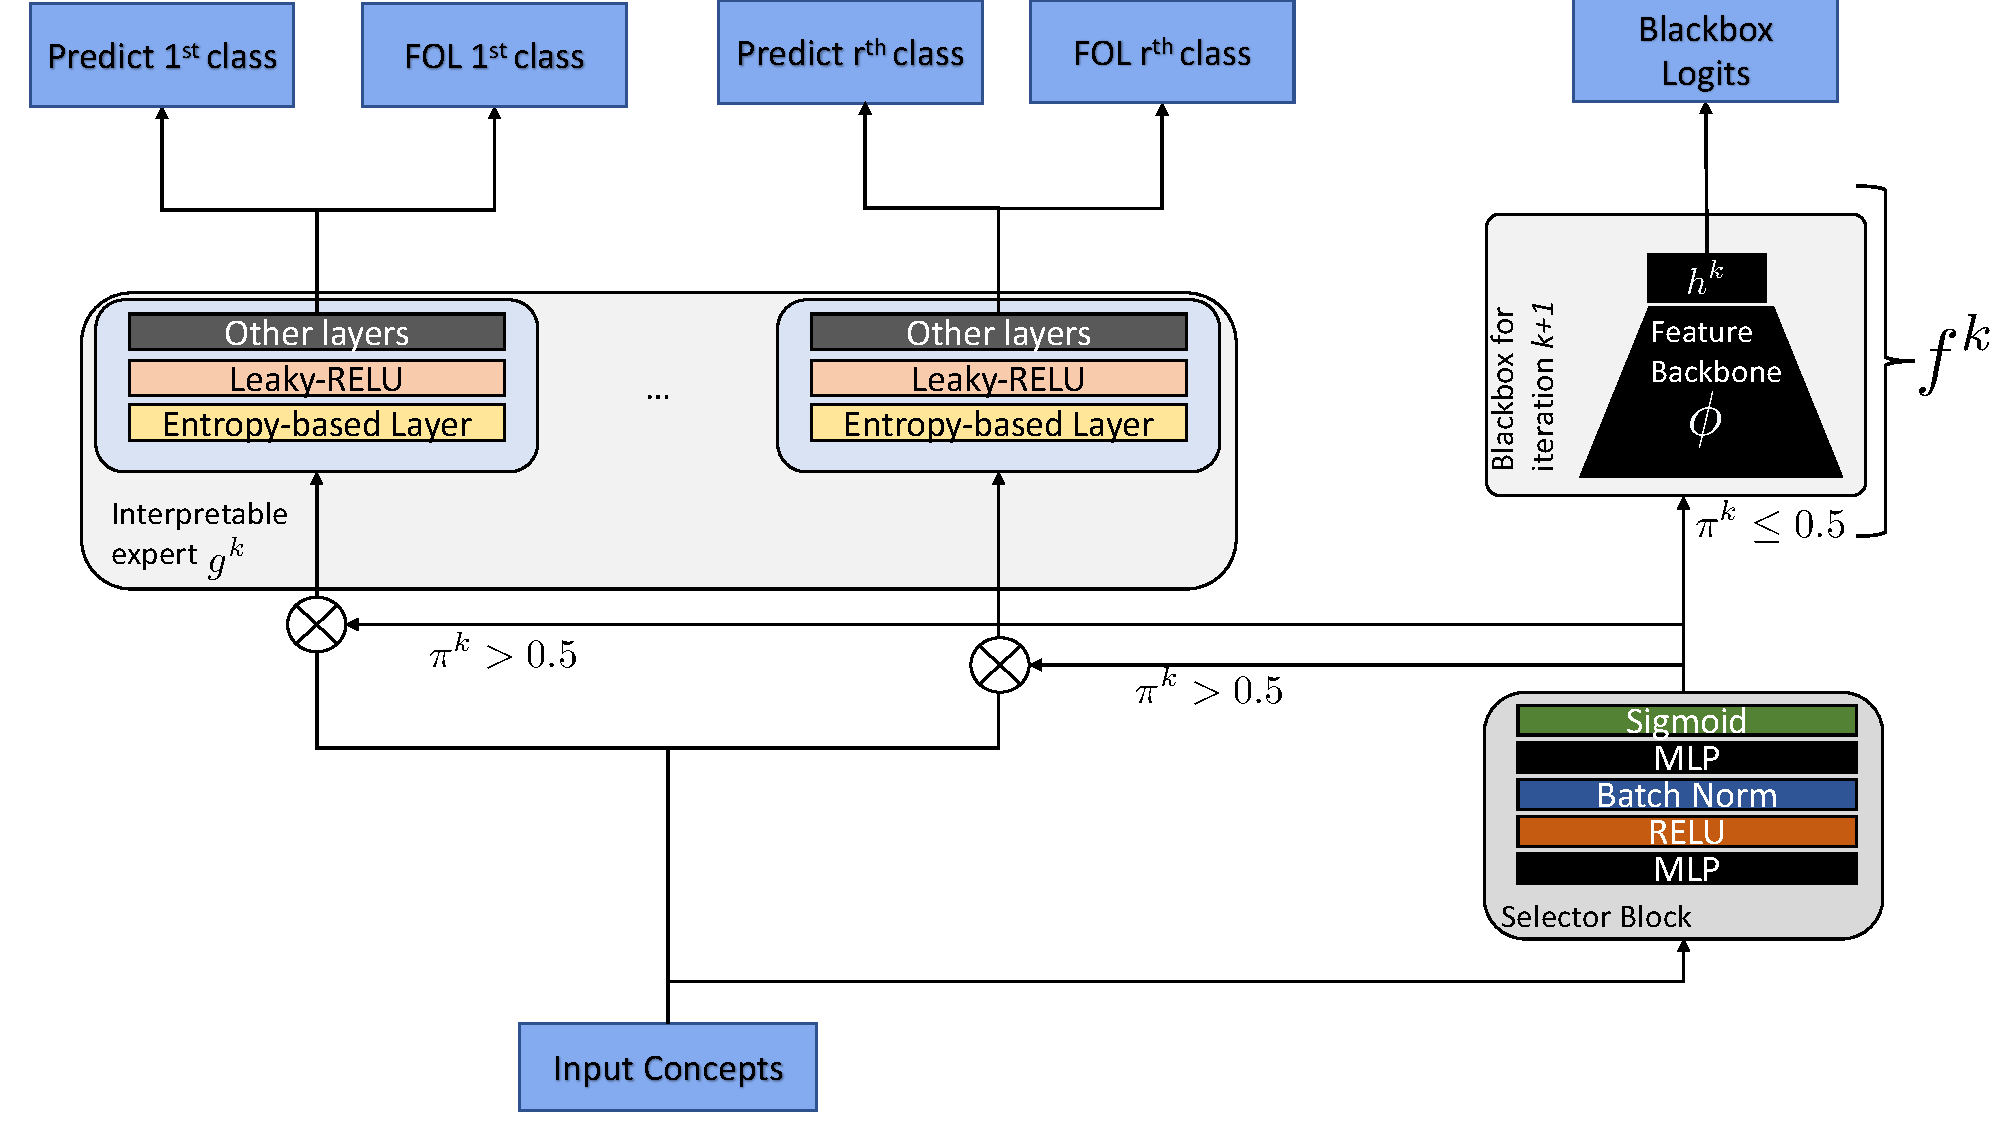
\includegraphics[width=1\textwidth]
{figures/Supp/Architecture.pdf}
\caption{Architecture of MoIE. In an iteration $k$ during inference, the selector routes the samples to go through the interpretable expert $g^k$ if the probability $\pi^k \ge 0.5$. If $\pi^k < 0.5$, the selector routes the samples, through $f^k$, the Blackbox for iteration $k+1$. Note $f^k = h^k(\Phi(.)$ is an approximation of the residual $r^k = f^{k-1} - g^k$.  }
\label{fig:architecture}
\end{figure}

\begin{algorithm}[h]
   \caption{\emph{Route, interpret} and \emph{repeat} algorithm to generate FOL explanations locally.}
   \label{algo: train}
\begin{algorithmic}[1]
   \STATE {\bfseries Input:} Complete tuple: \{$x_j$, $y_j$, $c_j$\}$_{j=1}^n$; initial blackbox $f^0 = h^0(\Phi(.))$; K as the total iterations; Coverages $\tau_1, \dots ,\tau_K$.
   \STATE {\bfseries Output:} Sparse mixture of experts and their selectors $\{g^k, \pi^k\}_{k=1}^K$ and the final residual $f^K = h^K(\Phi(.))$
   \STATE Fix $\Phi$.
   \FOR{\texttt{$k=1 \dots K $}}
       \STATE  Fix $\pi^1 \dots \pi^{k-1}$.
       \STATE Minimize $\mathcal{L}^k$ using equation \ref{equ:final_loss_g} to learn $\pi^k$ and $g^k$.
       \STATE Calculate $r^k = f^{k-1}(.) - g^k(.)$
       \STATE Minimize equation \ref{equ: residual} to learn $f^k(.)$, the new blackbox for the next iteration $k+1$.
       \ENDFOR
        \FOR{\texttt{$k=1 \dots K $}}
            \FOR{sample $j$ in \texttt{test-set}}
                \REPEAT
                    \STATE Initialize \texttt{sub\_select\_concept} = $True$
                    \STATE Initialize the \texttt{percentile\_threshold} = $99$.
                    \STATE Retrieve the predicted class label of sample $j$ from the expert $k$ as: $\hat{y}_j = g^k(c_j)$
                    \STATE Create a mask vector $m_j$. $m_j[i] = 1$ if 
                    $\Tilde{\alpha}[\hat{y}_j][i] \geq$ percentile$(\Tilde{\alpha}[\hat{y}_j]$, \texttt{percentile\_threshold}$)$ and $0$ otherwise. Specifically, the $i^{th}$ entry in $m_j$ is one if the $i^{th}$ value of the attention score $\Tilde{\alpha}[\hat{y}_j]$ is greater than (\texttt{percentile\_attention})$^{th}$ percentile. 
                    \STATE Subselect the concept vector as $\Tilde{c}_j$ as: $\Tilde{c}_j = c_j\odot m_j$
                    \IF{$g^k(\Tilde{c}_j) \neq \hat{y}_j$}
                        \STATE \texttt{percentile\_threshold} = \texttt{percentile\_threshold} - 1
                        \STATE \texttt{sub\_select\_concept} = $false$
                    \ENDIF
                \UNTIL \texttt{sub\_select\_concept} is $True$
                \STATE Using the subselected concept vector $\Tilde{c_j}$, construct the FOL expression of the $j^{th}$ sample as suggested by~\cite{barbiero2022entropy}.
            \ENDFOR
    \ENDFOR
\end{algorithmic}
\end{algorithm}

\cref{algo: train} explains the overall training procedure of our method.~\cref{fig:architecture} displays the architecture of our model in iteration $k$.


% \begin{algorithm}
% 	\caption{Training the MoIE to generate FOL explanations locally.} 
% 	\label{algo: train}
% 	\hspace*{\algorithmicindent} \textbf{Input:}  
%         {
%             Training set: \{$\mathcal{X}$, $\mathcal{Y}$, $\mathcal{S}$\}; trained blackbox $f^0 = h^0(\phi(.))$ using supervision of $\mathcal{Y}$; K as the \# iterations; Coverages $\tau_1, \dots ,\tau_k$
%         } \\
%         \hspace*{\algorithmicindent} \textbf{Output:}  
%         {
%             Sparse mixture of experts and their selectors $\{g^k, \pi^k\}_{k=1}^K$, 
%         }
% 	\begin{algorithmic}[1]
%         \State Fix $\phi$.
%         \State Train $t$ by minimizing BinaryCrossEnt($t(\phi(\boldsymbol{x})$, $\mathcal{S}$)
%         \State Form a concept bank $\mathcal{C}$ with p concepts after discarding the concepts whose validation auroc (accuracy) $\leq$ 0.7 (70\%)
%         \For{\texttt{iteration $k=1 \dots K $}}
%             \State Fix $\pi^1 \dots \pi^{k-1}$.
%             \State Minimize $\mathcal{L}^k$ using equation \ref{equ:final_loss_g} to learn $\pi^k$ and $g^k$.
%             \State Calculate $r^k = f^{k-1}(.) - g^k(.)$
%             \State Minimize equation \ref{equ: residual} to learn $f^k(.)$, the new blackbox for the next iteration $k+1$
%         \EndFor
%         \For{\texttt{experts $k=1 \dots K $}}
%             \For{\texttt{each sample in the test-set}}
%                 \State \label{12}Sort the concepts according to their attention scores from different experts in descending order.
%                 \State Initialise FOL\_bucket as empty list.
%                 \State Select one concept $\{c^i\}_{i=1}^p$ at a time from the sorted concept bank in step \ref{12} until 
%                 \hspace*{\algorithmicindent} \quad $g(c^i$) = g($\boldsymbol{c}$) and add those concepts in the  FOL\_bucket.
%                 \State Construct the FOL expression from FOL\_bucket using \cite{barbiero2022entropy}.
%             \EndFor
%         \EndFor
% 	\end{algorithmic} 
% \end{algorithm}




\subsection{Dataset}
\label{app:dataset}
\paragraph{CUB-200}
The Caltech-UCSD Birds-200-2011 (\cite{wah2011caltech}) is a fine-grained classification dataset comprising 11788 images and 312 noisy visual concepts. The aim is to classify the correct bird species from 200 possible classes. We adopted the strategy discussed in~\cite{barbiero2022entropy} to extract 108 denoised visual concepts. Also, we utilize training/validation splits shared in \cite{barbiero2022entropy}. Finally, we use the state-of-the-art classification models Resnet-101 (\cite{he2016deep}) and Vision-Transformer (VIT) (\cite{wang2021feature}) as the blackboxes $f^0$. 

% For the baseline, we train the convolution layers and the transformer encoder layers of Resnet-101 and the vision transformer respectively to learn the mapping $\mathcal{X} \rightarrow \mathcal{C}$ from scratch. Finally we used the concepts extracted in the previous 

\paragraph{Animals with attributes2 (Awa2)}
 AwA2 dataset \cite{xian2018zero} consists of 37322 images of total 50 animals classes with 85 numeric attribute. We use the state-of-the-art classification models Resnet-101 (\cite{he2016deep}) and Vision-Transformer (VIT) (\cite{wang2021feature}) as the blackboxes $f^0$.

\paragraph{HAM10000}
HAM10000 (\cite{tschandl2018ham10000}) is a classification dataset aiming to classify a skin lesion benign or malignant. Following \cite{daneshjou2021disparities}, we use Inception \cite{szegedy2015going} model, trained on this dataset as the blackbox $f^0$. We follow the strategy in \cite{lucieri2020interpretability} to extract the 8 concepts from the Derm7pt (\cite{kawahara2018seven}) dataset.

\paragraph{SIIM-ISIC}
To test a real-world transfer learning use case, we evaluate the
model trained on HAM10000 on a subset of the SIIM-ISIC\cite{rotemberg2021patient}) Melanoma Classification dataset. We use
the same concepts described in the HAM10000 dataset.

\paragraph{MIMIC-CXR} We use  220,763 frontal images from the MIMIC-CXR dataset \cite{12_johnsonmimic} aiming to classify effusion. We obtain the anatomical and observation concepts from the RadGraph annotations in RadGraph’s inference dataset (\cite{10_jain2021radgraph}), automatically generated by DYGIE++ (\cite{23_wadden-etal-2019-entity}). We use the test-train-validation splits from \cite{yu2022anatomy} and Densenet121 \cite{huang2017densely} as the blackbox $f^0$. 






\subsection{Estimation of completeness score}
\label{app:completeness}


Let $f^0(x)=h^0(\Phi(\boldsymbol{x})$ is the initial Blackbox as per~\cref{sec:method}. The Concept completeness paper~\cite{yeh2019concept} assumes $\Phi(\boldsymbol{x}) \in \mathbb{R}^l$ (\st $l=T.d$) to be a concatanation of $[\phi(\boldsymbol{x}_1), \phi(\boldsymbol{x}_2), \dots, \phi(\boldsymbol{x}_T)]$ \st $\phi(\boldsymbol{x}) \in \mathbb{R}^d$. Recall we utilize $t$ to learn the concepts $\mathcal{C}$ with $N_c$ being the total number of concepts per image. So the parameters of $t$, represented by $\omega_1, \omega_2, \dots \omega_{N_c}$ \st $\omega_i \in \mathbb{R}^d$ represent linear direction in the embedding space $\phi(.) \in \mathbb{R}^d$. Next, we compute the concept product $v_c(\boldsymbol{x}_t)(<\phi(\boldsymbol{x}_t), \omega_j>)_{j=1}^{N_c}$, denoting the similarity between the image embedding and linear direction of $j^{th}$ concept. Finally, we normalize $v_c(.)$ to obtain the concept score as 
$v_v(\boldsymbol{x}) = \big(\frac{v_c(\boldsymbol{x_t})}{||v_c(\boldsymbol{x}_t)||_2}\big)_{t=1}^T \in \mathbb{R}^{T.{N_c}}$.

Next for a Blackbox $f^0(x)=h^0(\Phi(\boldsymbol{x})$, set of concepts $c_1, c_2, \dots c_{N_c}$ and their linear direction  $\omega_1, \omega_2, \dots \omega_{N_c}$ in the embedding space and, we compute the completeness score as:

\begin{align}
\eta_{f^0} = \frac{\text{sup}_\Gamma \mathbb{P}_{\boldsymbol{x}, y \sim V}
[y = \operatorname*{arg\,max}_{y'}h^0_{y'}(\Gamma(v_c(\boldsymbol{x})))] - a_r}{
\mathbb{P}_{\boldsymbol{x}, y \sim V}
[y = \operatorname*{arg\,max}_{y'}f^0_{y'}(\boldsymbol{x})] - a_r
},
\end{align}

where $V$ is the validation set and $\Gamma : \mathbb{R}^{T.m} \rightarrow \mathbb{R}^l$, projection from the concept score to the embedding space$\Phi$. For CUB-200 and Awa2 we estimate $\mathbb{P}_{\boldsymbol{x}, y \sim V}
[y = \operatorname*{arg\,max}_{y'}h^0_{y'}(\Gamma(v_c(\boldsymbol{x})))]$ as the best accuracy using the given concepts and $a_r$ is the random accuracy. For HAM10000, we estimate the same as the best AUROC. Completeness score indicates the consistency between the prediction based just on concepts and the given Blackbox$f^0$. If the identified concepts are sufficiently rich, label prediction will be similar to the Blackbox, resulting in higher completeness scores for the concept set. In all our experiments, $\Gamma$ is a two-layer feedforward neural network with 1000 neurons.

To plot the completeness score in~\cref{fig:valid_concepts}a-c, we select the topN concepts iteratively representing the $N < N_c$ concepts most significant to the prediction of the interpretable model $g$. Recall we follow Entropy based linear neural network~\cite{barbiero2022entropy} as $g$. So each concept has an associated attention score, $\alpha$ in $g$~\cite{barbiero2022entropy}, denoting the importance of the concept for the prediction. We select the topN concepts based on the $N$ concepts with highest attention weights. We get the linear direction of these topN concepts from the parameters of the learned $t$ and project it to the embedding space $\Phi$ using $\Gamma$. If $\Gamma$ reconstructs the discriminative features from the concepts successfully, the concepts achieves high completeness scores, showing faithfulness with the Blackbox. Recall~\cref{fig:valid_concepts}a-c demonstrate that MoIE outperforms the baselines in terms of the completeness scores. This suggests that MoIE identifies rich instance-specific concepts than the baselines, being consistent with the Blackbox.

\subsection{Architectural details of symbolic experts and hyperparameters}
\label{app:g}



\cref{tab:bb_config} demonstrates different settings to train the Blackbox of CUB-200, Awa2 and MIMIC-CXR respectively. For the VIT-based backbone, we used the same hyperparameter setting used in the state-of-the-art Vit-B\_16 variant in \cite{wang2021feature}. To train $t$, we flatten the feature maps from the last convolutional block of $\Phi$ using ``Adaptive average pooling'' for CUB-200 and Awa2 datasets.For MIMIC-CXR and HAM10000, we flatten out the feature maps from the last convolutional block. For VIT-based backbones, we take the first block of representation from the encoder of VIT.  For HAM10000, we use the same Blackbox in \cite{yuksekgonul2022post}.~\cref{tab:g_config_cub_200},~\cref{tab:g_config_awa2},~\cref{tab:g_config_ham10k},~\cref{tab:g_config_mimic_cxr} enumerate all the different settings to train the interpretable experts for CUB-200, Awa2, HAM, and MIMIC-CXR respectively. All the residuals in different iterations follow the same settings as their blackbox counterparts.


% \begin{table}[h]
% \caption{Hyperparameter setting of interpretable experts ($g$) for ResNet-101-based Blackbox used by CUB-200}
% \label{table7}
% \begin{center}
% \begin{tabular}{l|l|l|l|l|l|l}
% \toprule 
%      {\textbf{Setting}} & {\textbf{Expert1}} & {\textbf{Expert2}} 
%      & {\textbf{Expert3}} & {\textbf{Expert4}} & {\textbf{Iteration5}}
%      & {\textbf{Iteration6}}\\
% \midrule 
%        Batch size              & 16 & 16 & 16 & 16 & 16 & 16   \\
%        \midrule 
%        Coverage ($\tau$)  & 0.2 & 0.2 & 0.2 & 0.2 & 0.2 & 0.2 \\
%        \midrule
%        Learning rate & 0.01 & 0.01 & 0.01 & 0.01 & 0.01 & 0.01 \\
%        \midrule 
%        Temperature \\ E-Lens ($T_{lens}$) & 0.7 & 0.7 & 0.7 & 0.7 & 0.7 & 0.7 \\
%        \midrule 
%        $\lambda_{lens}$ & 0.0001 & 0.0001 & 0.0001 & 0.0001 & 0.0001 & 0.0001 \\
%        \midrule
%        $\alpha_{KD}$ & 0.9 & 0.9 & 0.9 & 0.9 & 0.9 & 0.9 \\
%        \midrule
%        $T_{KD}$ & 10 & 10 & 10 & 10 &10 & 10 \\
%        \midrule
%        hidden neurons & 10 & 10 & 10 & 10 &10 & 10 \\
% \bottomrule
% \end{tabular}
% \end{center}
% \end{table}

% \begin{table}[h]
% \caption{Hyperparameter setting of interpretable experts ($g$) for VIT-based Blackbox used by CUB-200}
% \label{table7}
% \begin{center}
% \begin{tabular}{l|l|l|l|l|l|l}
% \toprule 
%      {\textbf{Setting}} & {\textbf{Iteration1}} & {\textbf{Iteration2}} 
%      & {\textbf{Iteration3}} & {\textbf{Iteration4}} & {\textbf{Iteration5}}
%      & {\textbf{Iteration6}}\\
% \midrule 
%        Batch size              & 16 & 16 & 16 & 16 & 16 & 16   \\
%        \midrule 
%        Coverage ($\tau$)  & 0.2 & 0.2 & 0.2 & 0.2 & 0.2 & 0.2 \\
%        \midrule
%        Learning rate & 0.01 & 0.01 & 0.01 & 0.01 & 0.01 & 0.01 \\
%        \midrule 
%        Temperature \\ E-Lens ($T_{lens}$) & 6.0 & 6.0 & 6.0 & 6.0 & 6.0 & 6.0 \\
%        \midrule 
%        $\lambda_{lens}$ & 0.0001 & 0.0001 & 0.0001 & 0.0001 & 0.0001 & 0.0001 \\
%        \midrule
%        $\alpha_{KD}$ & 0.99 & 0.99 & 0.99 & 0.99 & 0.99 & 0.99 \\
%        \midrule
%        $T_{KD}$ & 10 & 10 & 10 & 10 &10 & 10 \\
%        \midrule
%        hidden neurons & 10 & 10 & 10 & 10 &10 & 10 \\
% \bottomrule
% \end{tabular}
% \end{center}
% \end{table}

% \begin{table}[h]
% \caption{Hyperparameter setting of interpretable experts ($g$) for VIT-based Blackbox used by CUB-200}
% \label{table7}
% \begin{center}
% \begin{tabular}{l|l|l|l|l|l|l}
% \toprule 
%      {\textbf{Setting}} & {\textbf{Iteration1}} & {\textbf{Iteration2}} 
%      & {\textbf{Iteration3}} & {\textbf{Iteration4}} & {\textbf{Iteration5}}
%      & {\textbf{Iteration6}}\\
% \midrule 
%        Batch size              & 16 & 16 & 16 & 16 & 16 & 16   \\
%        \midrule 
%        Coverage ($\tau$)  & 0.2 & 0.2 & 0.2 & 0.2 & 0.2 & 0.2 \\
%        \midrule
%        Learning rate & 0.01 & 0.01 & 0.01 & 0.01 & 0.01 & 0.01 \\
%        \midrule 
%        Temperature \\ E-Lens ($T_{lens}$) & 6.0 & 6.0 & 6.0 & 6.0 & 6.0 & 6.0 \\
%        \midrule 
%        $\lambda_{lens}$ & 0.0001 & 0.0001 & 0.0001 & 0.0001 & 0.0001 & 0.0001 \\
%        \midrule
%        $\alpha_{KD}$ & 0.99 & 0.99 & 0.99 & 0.99 & 0.99 & 0.99 \\
%        \midrule
%        $T_{KD}$ & 10 & 10 & 10 & 10 &10 & 10 \\
%        \midrule
%        hidden neurons & 10 & 10 & 10 & 10 &10 & 10 \\
% \bottomrule
% \end{tabular}
% \end{center}
% \end{table}



\begin{table}[h]
\caption{Hyperparameter setting of different convolution-based Blackboxes used by CUB-200, Awa2 and MIMIC-CXR}
\label{tab:bb_config}
\begin{center}
\begin{tabular}{l c c c}
\toprule 
     {\textbf{Setting}} & {\textbf{CUB-200}} & {\textbf{Awa2}} & 
    {\textbf{MIMIC-CXR}}\\
\midrule 
       Backbone              & ResNet-101 & ResNet-101 & DenseNet-121  \\
       % \midrule 
       Pretrained on ImageNet      & True &True & True \\
       % \midrule 
       Image size            & 448 & 224 & 512 \\
       % \midrule 
       Learning rate         & 0.001 & 0.001 & 0.01 \\
       % \midrule 
       Optimization          & SGD & Adam & SGD \\
       % \midrule 
       Weight-decay      & 0.00001 & 0 & 0.0001 \\
       % \midrule 
       Epcohs             & 95 & 90 & 50 \\
       % \midrule 
       Layers used as $\Phi$ &  \makecell{till 4$^{th}$ ResNet \\Block} &  \makecell{till 4$^{th}$ ResNet \\Block} &  \makecell{till 4$^{th}$ DenseNet \\Block} \\
       % \midrule 
       Flattening type for the input to $t$    &  \makecell{Adaptive average \\pooling} &  \makecell{Adaptive average \\pooling} & Flatten \\
\bottomrule
\end{tabular}
\end{center}
\end{table}


\begin{table}[h]
\caption{Hyperparameter setting of interpretable experts ($g$) trained on ResNet-101 (top) and VIT (bottom) blackboxes for the CUB-200 dataset}
\label{tab:g_config_cub_200}
\begin{center}
\begin{tabular}{l|c|c|c|c|c|c}
\toprule 
    \thead{\textbf{Settings based on dataset}} & \thead{\textbf{Expert1}} & \thead{\textbf{Expert2}} 
    & \thead{\textbf{Expert3}} & \thead{\textbf{Expert4}} & \thead{\textbf{Expert5}} & \thead{\textbf{Expert6}}\\
     % {\textbf{Setting}} & {\textbf{Expert1}} & {\textbf{Expert2}} 
     % & {\textbf{Expert3}} & {\textbf{Expert4}} & {\textbf{Expert5}}
     % & {\textbf{Expert6}}\\
\midrule 
        CUB-200 (ResNet-101)              &    &   &  & &  & \\
       \quad + Batch size              & 16 & 16 & 16 & 16 & 16 & 16   \\
        
       \quad + Coverage ($\tau$)  & 0.2 & 0.2 & 0.2 & 0.2 & 0.2 & 0.2 \\
       
       \quad + Learning rate & 0.01 & 0.01 & 0.01 & 0.01 & 0.01 & 0.01 \\
       
       \quad + $\lambda_{lens}$ & 0.0001 & 0.0001 & 0.0001 & 0.0001 & 0.0001 & 0.0001 \\
    
       \quad +$\alpha_{KD}$ & 0.9 & 0.9 & 0.9 & 0.9 & 0.9 & 0.9 \\
       \quad + $T_{KD}$ & 10 & 10 & 10 & 10 &10 & 10 \\
       \quad +hidden neurons & 10 & 10 & 10 & 10 &10 & 10 \\
       \quad +$\lambda_s$ & 32 & 32 & 32 & 32 & 32 & 32 \\
       \quad + $T_{lens}$ & 0.7 & 0.7 & 0.7 & 0.7 & 0.7 & 0.7 \\
\midrule 
        CUB-200 (VIT)            &    &   &  & &  & \\
       \quad + Batch size              & 16 & 16 & 16 & 16 & 16 & 16   \\
        
       \quad + Coverage ($\tau$)  & 0.2 & 0.2 & 0.2 & 0.2 & 0.2 & 0.2 \\
       
       \quad + Learning rate & 0.01 & 0.01 & 0.01 & 0.01 & 0.01 & 0.01 \\
       
       
       \quad + $\lambda_{lens}$ & 0.0001 & 0.0001 & 0.0001 & 0.0001 & 0.0001 & 0.0001 \\
    
       \quad +$\alpha_{KD}$ & 0.99 & 0.99 & 0.99 & 0.99 & 0.99 & 0.99 \\
       \quad + $T_{KD}$ & 10 & 10 & 10 & 10 &10 & 10 \\
       \quad +hidden neurons & 10 & 10 & 10 & 10 &10 & 10 \\
       \quad +$\lambda_s$ & 32 & 32 & 32 & 32 & 32 & 32 \\
       \quad +$T_{lens}$ & 6.0 & 6.0 & 6.0 & 6.0 & 6.0 & 6.0 \\
\bottomrule
\end{tabular}
\end{center}
\end{table}

\begin{table}[h]
\caption{Hyperparameter setting of interpretable experts ($g$) trained on ResNet-101 (top) and VIT (bottom) blackboxes for the Awa2 dataset}
\label{tab:g_config_awa2}
\begin{center}
\begin{tabular}{l|c|c|c|c|c|c}
\toprule 
    \thead{\textbf{Settings based on dataset}} & \thead{\textbf{Expert1}} & \thead{\textbf{Expert2}} 
    & \thead{\textbf{Expert3}} & \thead{\textbf{Expert4}} & \thead{\textbf{Expert5}} & \thead{\textbf{Expert6}}\\
     % {\textbf{Setting}} & {\textbf{Expert1}} & {\textbf{Expert2}} 
     % & {\textbf{Expert3}} & {\textbf{Expert4}} & {\textbf{Expert5}}
     % & {\textbf{Expert6}}\\
\midrule 
        Awa2 (ResNet-101)              &    &   &  & &  & \\
       \quad + Batch size              & 30 & 30 & 30 & 30 & - & -   \\
        
       \quad + Coverage ($\tau$)  & 0.4 & 0.35 & 0.35 & 0.25 & - & - \\
       
       \quad + Learning rate & 0.001 & 0.001 & 0.001 & 0.001 & - & - \\
       
       \quad + $\lambda_{lens}$ & 0.0001 & 0.0001 & 0.0001 & 0.0001 & - & - \\
    
       \quad +$\alpha_{KD}$ & 0.9 & 0.9 & 0.9 & 0.9 & - & - \\
       \quad + $T_{KD}$ & 10 & 10 & 10 & 10 & - & - \\
       \quad +hidden neurons & 10 & 10 & 10 & 10 & - & - \\
       \quad +$\lambda_s$ & 32 & 32 & 32 & 32 & - & - \\
       \quad + $T_{lens}$ & 0.7 & 0.7 & 0.7 & 0.7 & - & - \\
\midrule 
        Awa2 (VIT)            &    &   &  & &  & \\
       \quad + Batch size              & 30 & 30 & 30 & 30 & 30 & 30   \\
        
       \quad + Coverage ($\tau$)  & 0.2 & 0.2 & 0.2 & 0.2 & 0.2 & 0.2 \\
       
       \quad + Learning rate & 0.01 & 0.01 & 0.01 & 0.01 & 0.01 & 0.01 \\
       
       
       \quad + $\lambda_{lens}$ & 0.0001 & 0.0001 & 0.0001 & 0.0001 & 0.0001 & 0.0001 \\
    
       \quad +$\alpha_{KD}$ & 0.99 & 0.99 & 0.99 & 0.99 & 0.99 & 0.99 \\
       \quad + $T_{KD}$ & 10 & 10 & 10 & 10 &10 & 10 \\
       \quad +hidden neurons & 10 & 10 & 10 & 10 &10 & 10 \\
       \quad +$\lambda_s$ & 32 & 32 & 32 & 32 & 32 & 32 \\
       \quad + $T_{lens}$ & 6.0 & 6.0 & 6.0 & 6.0 & 6.0 & 6.0 \\
\bottomrule
\end{tabular}
\end{center}
\end{table}


\begin{table}[h]
\caption{Hyperparameter setting of interpretable experts ($g$) for the dataset HAM10000}
\label{tab:g_config_ham10k}
\begin{center}
\begin{tabular}{l|c|c|c|c|c|c}
\toprule 
    \thead{\textbf{Settings based on dataset}} & \thead{\textbf{Expert1}} & \thead{\textbf{Expert2}} 
    & \thead{\textbf{Expert3}} & \thead{\textbf{Expert4}} & \thead{\textbf{Expert5}}
    & {\textbf{Expert6}}\\
     % {\textbf{Setting}} & {\textbf{Expert1}} & {\textbf{Expert2}} 
     % & {\textbf{Expert3}} & {\textbf{Expert4}} & {\textbf{Expert5}}
     % & {\textbf{Expert6}}\\
\midrule 
        HAM10000 (Inception-V3)              &    &   &  & & &  \\
       \quad + Batch size              & 32 & 32 & 32 & 32 & 32&  32   \\
        
       \quad + Coverage ($\tau$)  & 0.4 & 0.2 & 0.2 & 0.2 & 0.1&  0.1\\
       
       \quad + Learning rate & 0.01 & 0.01 & 0.01 & 0.01 & 0.01& 0.01 \\
       
       \quad + $\lambda_{lens}$ & 0.0001 & 0.0001 & 0.0001 & 0.0001 & 0.0001 &  0.0001\\
    
       \quad +$\alpha_{KD}$ & 0.9 & 0.9 & 0.9 & 0.9 & 0.9& 0.9\\
       \quad + $T_{KD}$ & 10 & 10 & 10 & 10 & 10& 10 \\
       \quad +hidden neurons & 10 & 10 & 10 & 10 & 10& 10\\
       \quad +$\lambda_s$ & 64 & 64 & 64 & 64 & 64& 64  \\
       \quad + $T_{lens}$ & 0.7 & 0.7 & 0.7 & 0.7 & 0.7& 0.7 \\
\bottomrule
\end{tabular}
\end{center}
\end{table}

\begin{table}[H]
\caption{Hyperparameter setting of interpretable experts ($g$) for the dataset MIMIC-CXR}
\label{tab:g_config_mimic_cxr}
\begin{center}
\begin{tabular}{l|c|c|c}
\toprule 
    \thead{\textbf{Settings based on dataset}} & \thead{\textbf{Expert1}} & \thead{\textbf{Expert2}} 
    & \thead{\textbf{Expert3}} \\
     % {\textbf{Setting}} & {\textbf{Expert1}} & {\textbf{Expert2}} 
     % & {\textbf{Expert3}} & {\textbf{Expert4}} & {\textbf{Expert5}}
     % & {\textbf{Expert6}}\\
\midrule 
        Effusion-MIMIC-CXR (DenseNet-121)              &    &   &     \\
       \quad + Batch size              & 1028 & 1028 & 1028     \\
        
       \quad + Coverage ($\tau$)  & 0.6 & 0.2 & 0.15   \\
       
       \quad + Learning rate & 0.01 & 0.01 & 0.01 \\
       
       \quad + $\lambda_{lens}$ & 0.0001 & 0.0001 & 0.0001  \\
    
       \quad +$\alpha_{KD}$ & 0.99 & 0.99 & 0.99  \\
       \quad + $T_{KD}$ & 20 & 20 & 20   \\
       \quad +hidden neurons & 20, 20 & 20, 20 & 20, 20  \\
       \quad +$\lambda_s$ & 96 & 128 & 256   \\
       \quad +$T_{lens}$ & 7.6 & 7.6 & 7.6 \\
\bottomrule
\end{tabular}
\end{center}
\end{table}



\subsection{Flow diagram to eliminate shotcut}
\label{app:shortcut}
\cref{fig:spurious_flow} shows the flow digram to eliminate shortcut.
\begin{figure*}[h]
\centering
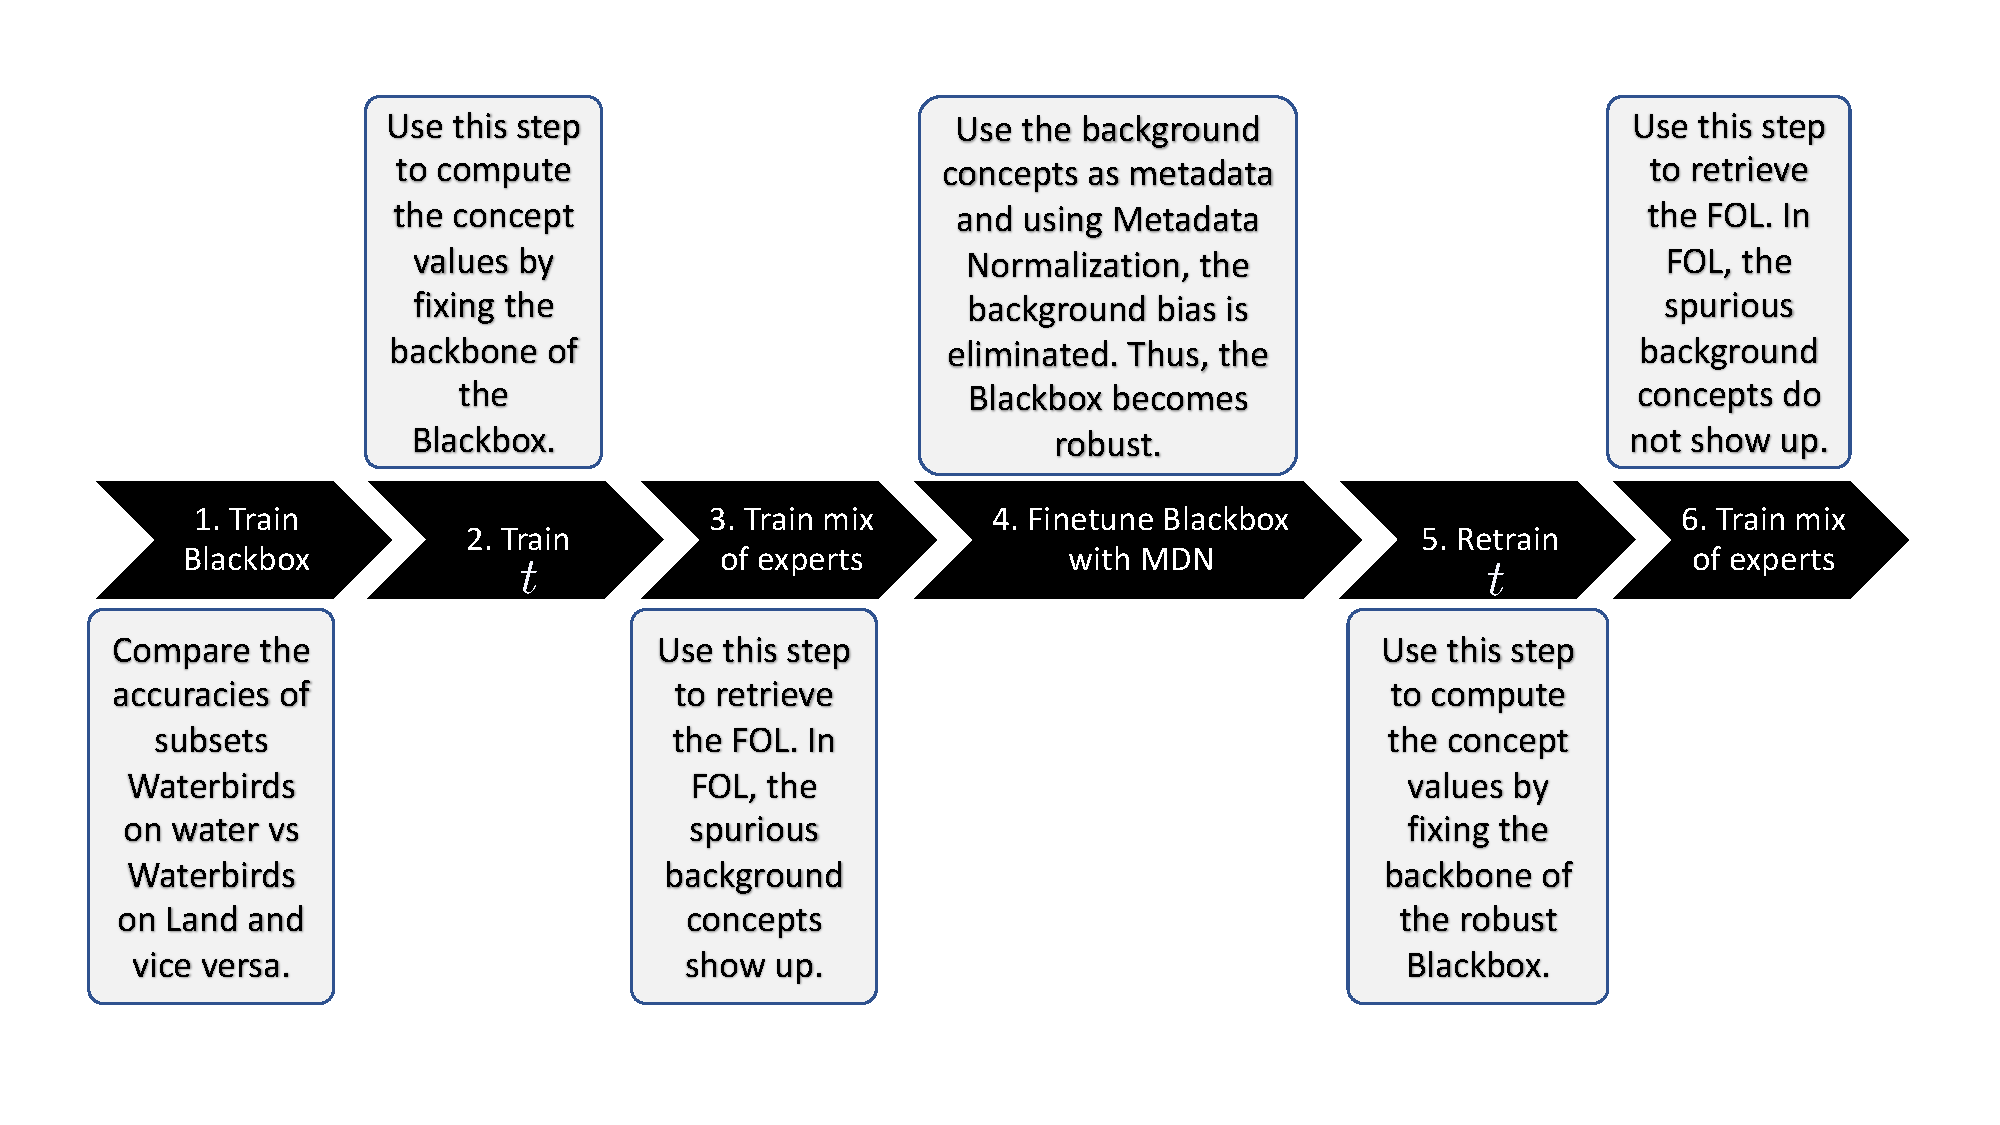
\includegraphics[width=1.0\textwidth]
{figures/Supp/Spurious_Flow.pdf}
\caption{The flow diagram to eliminate the shortcut from vision datasets using FOL by MoIE.}
\label{fig:spurious_flow}
\end{figure*}


\subsection{More Results}
\subsubsection{Comparison with other interpretable by design baselines}
\label{app:more_baselines}
\begin{table}[H]
\caption{Comparing the performance of MoIE with additional interpretable by design baselines.
}
\fontsize{7.5pt}{0.20cm}\selectfont
\label{tab:performance_app}
% \vskip 0.15in
\begin{center}
% \begin{small}
% \begin{sc}
\begin{tabular}{p{23em} c c c c}
\toprule 
        \textbf{MODEL} & \multicolumn{3}{c}{\textbf{DATASET}} \\
       & CUB-200 (RESNET101) & AWA2 (RESNET101) & EFFUSION  \\
\midrule 
    BLACKBOX & 0.88 & 0.89 & 0.91 \\
\midrule 
ANTEHOC W SUP~\cite{sarkar2021inducing} & 0.71 & 0.85 & 0.75\\
ANTEHOC W/O SUP~\cite{sarkar2021inducing} & 0.64 & 0.81 & 0.70\\
HARD W AR~\cite{havasi2022addressing} & 0.81 & 0.84 & 0.73\\
HARD W/O AR~\cite{havasi2022addressing} & 0.78 & 0.81 & 0.71\\
\midrule
\textbf{OURS} \\
MoIE (COVERAGE) &\textbf{0.86} &
     \textbf{0.87}
     & \textbf{0.87} \\
MoIE + RESIDUAL &\textbf{0.84} &
     \textbf{0.86}
     & \textbf{0.86} \\
\bottomrule
\end{tabular}
% \end{sc}
% \end{small}
\end{center}
% \vskip -0.1in
\end{table}
~\cref{tab:performance_app} compares our method with several other interpretable by design baselines.


\subsubsection{Results of Effusion of MIMIC-CXR}
\label{app:mimic_cxr}
\begin{figure*}[h]
\centering
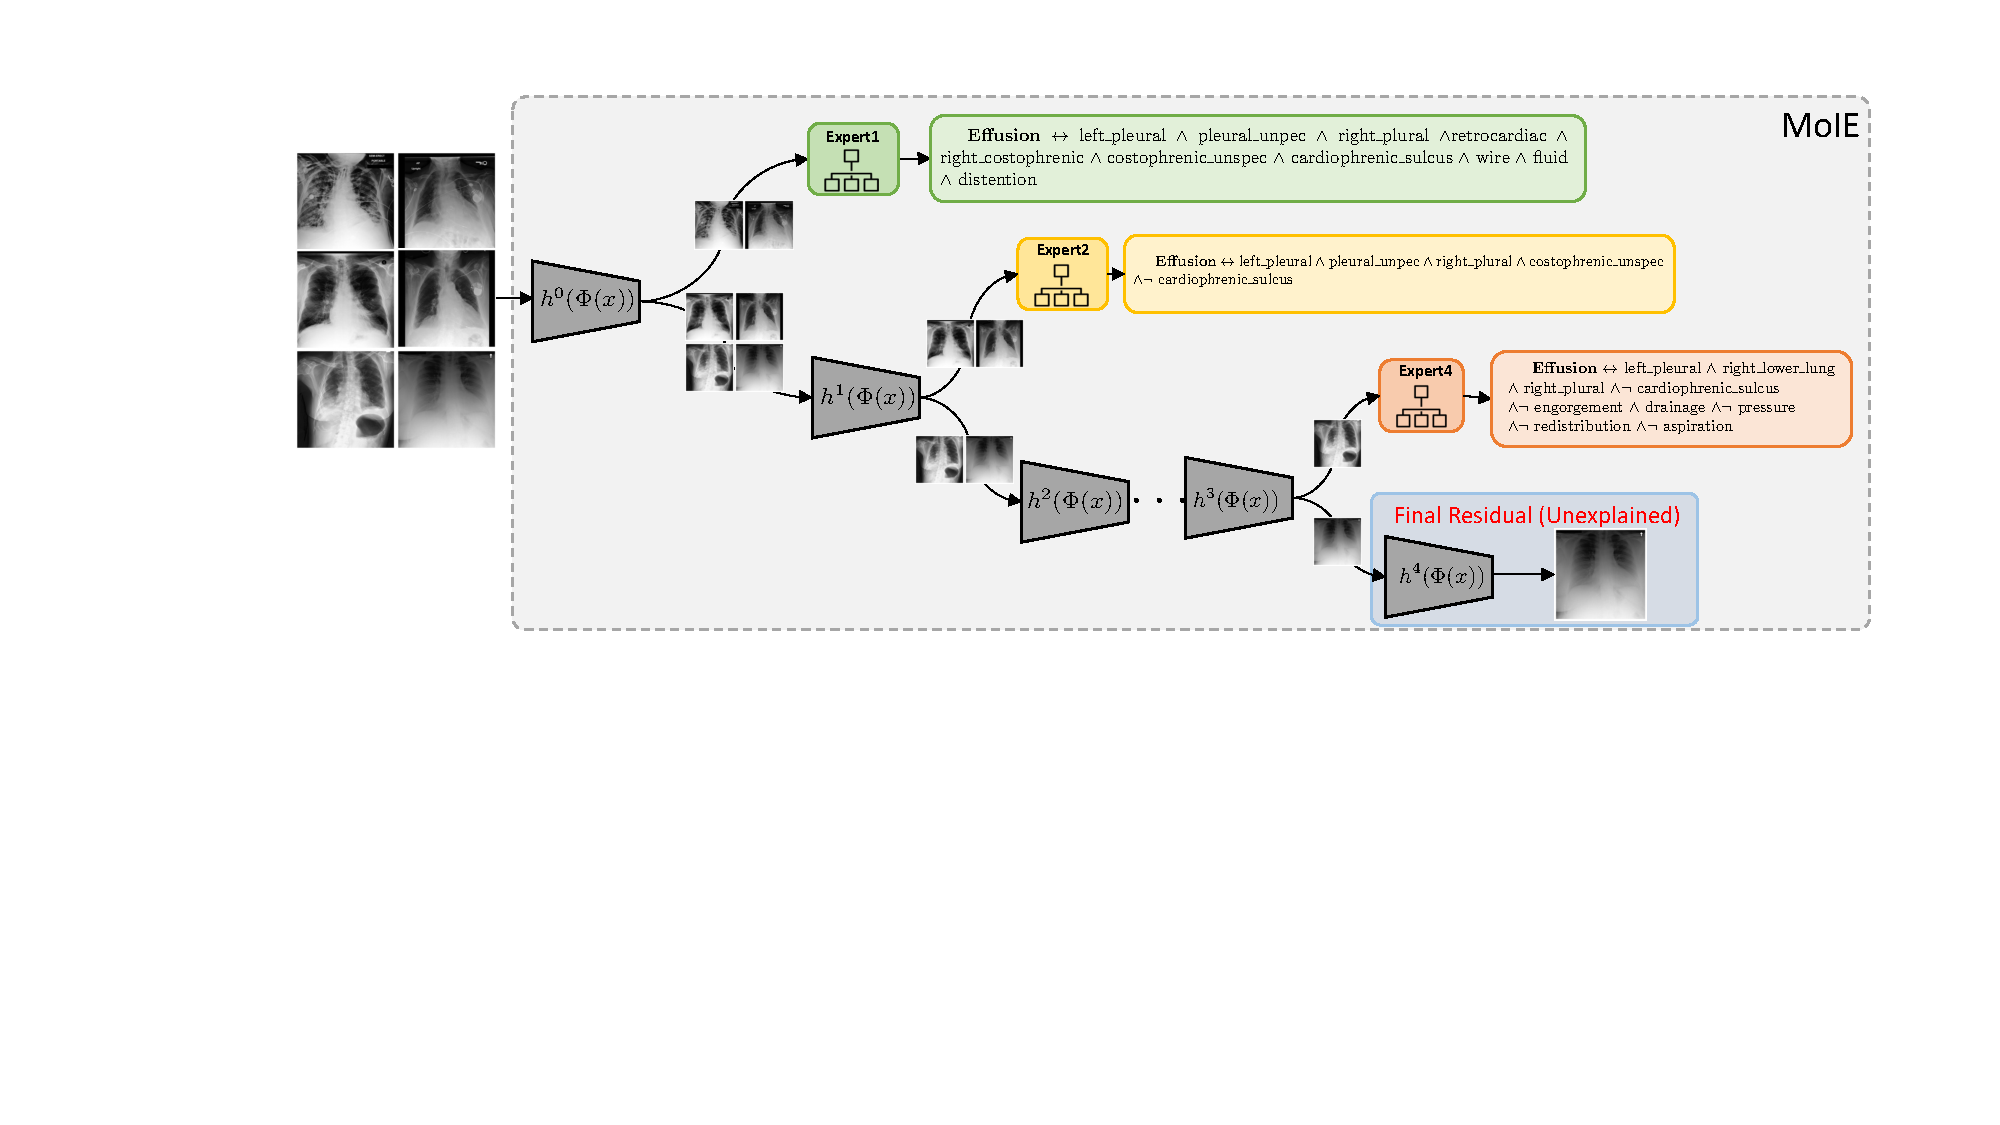
\includegraphics[width=1.0\textwidth]
{figures/Supp/mimic_concept_explanation.pdf}
\caption{Construction logical explanations of the samples of ``Effusion'' in the MIMIC-CXR dataset for various experts in MoIE at inference. The final residual covers the unexplained sample, which is ``harder'' to explain (indicated in \emph{red}).}
\label{fig:mimic_concept_explanation}
\end{figure*}

\begin{figure*}[h]
\centering
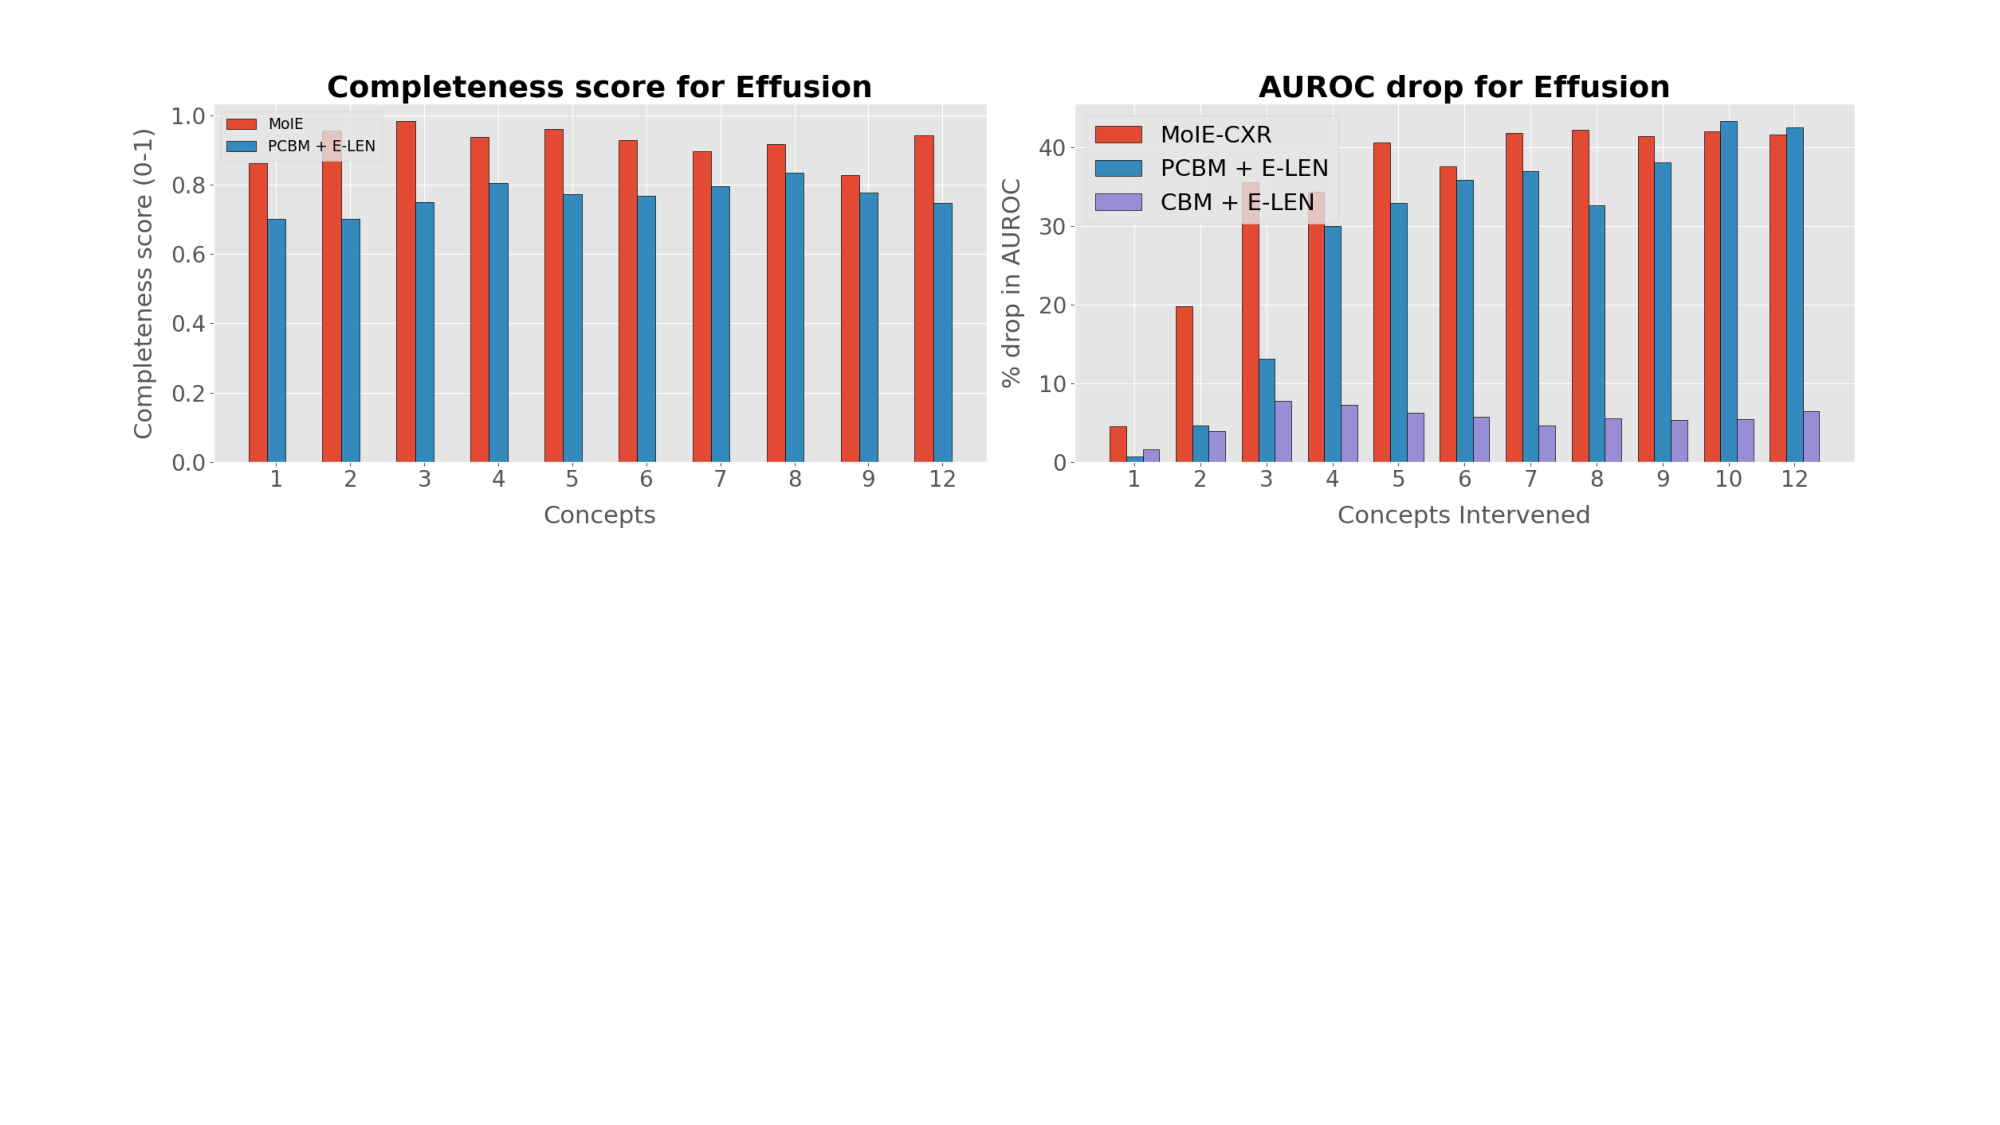
\includegraphics[width=1.0\textwidth]
{figures/Supp/mimic_concept_quant.pdf}
\caption{\textbf{(a)} Completeness scores for different significant concepts of Effusion.  \textbf{(b)} Drop in AUROC by zeroing out the concepts for Effusion.}
\label{fig:mimic_concept_quant}
\end{figure*}

\begin{figure*}[h]
\centering
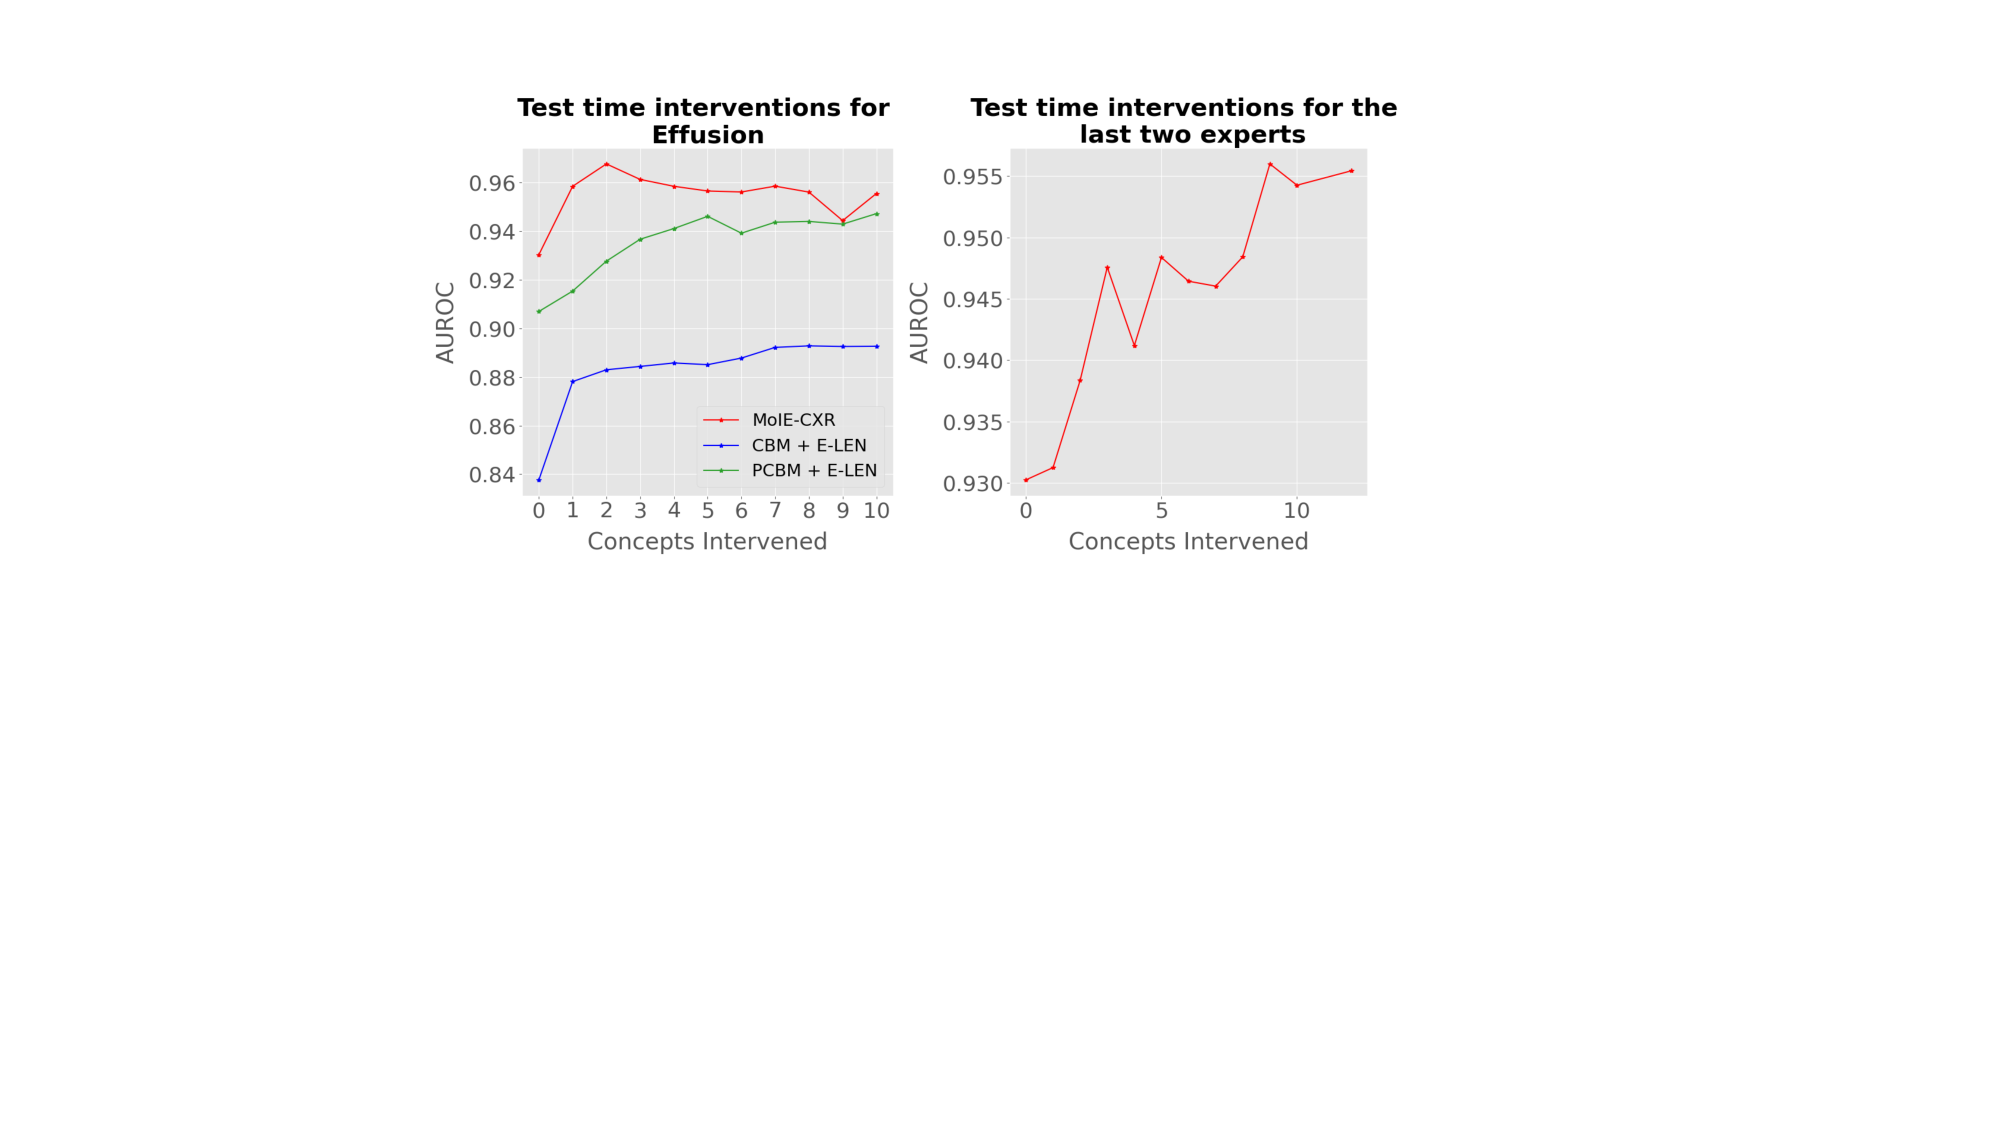
\includegraphics[width=1.0\textwidth]
{figures/Supp/mimic_concept_tti.pdf}
\caption{\textbf{(a)} Test time interventions of different concepts on all samples for Effusion.
\textbf{(b)} Test time interventions of different concepts on only the ``hard'' samples covered by the last two experts for Effusion}
\label{fig:mimic_concept_tti}
\end{figure*}

~\cref{fig:mimic_concept_explanation} demonstrates the diversity of instance-specific local FOL explanations of different concepts of MoIE and the final residual.~\cref{fig:mimic_concept_quant}(a) shows the completeness scores for different concepts.~\cref{fig:mimic_concept_quant}(b) shows the drop in AUROC while zeroing out different concepts. ~\cref{fig:mimic_concept_tti}(a) shows test time interventions of different concepts on all samples. ~\cref{fig:mimic_concept_tti}(b) shows test time interventions of different concepts on only the ``hard'' samples covered by the last two experts.




\subsubsection{Performance of experts and residual for ResNet-derived experts of Awa2 and CUB-200 datasets}
\label{app:resnet_cv}
\begin{figure}[h]
\centering
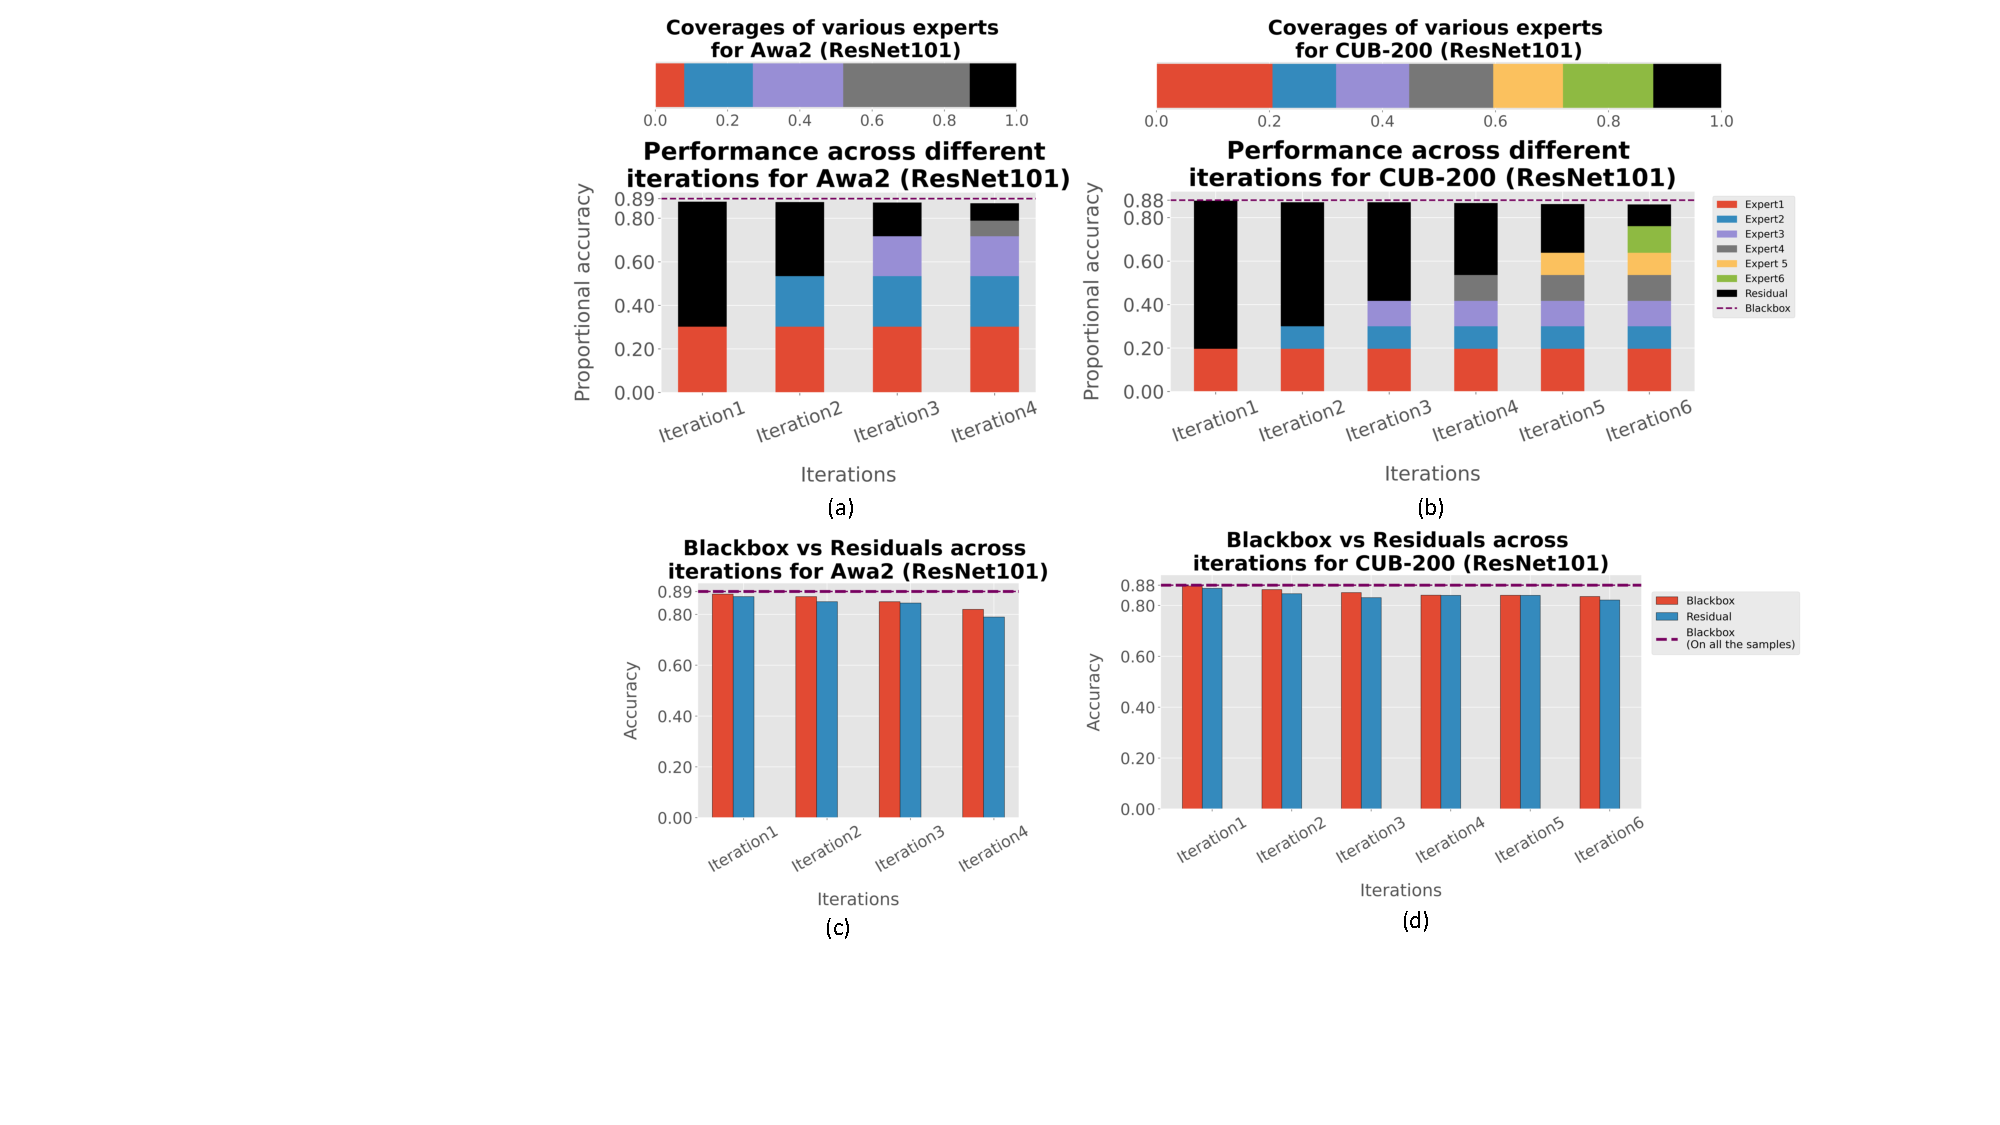
\includegraphics[width=1\linewidth]{figures/Supp/Expert_resnet.pdf}
\caption{The performances of experts and residuals across iterations for ResNet derived MoIE for CUB-200 and Awa2. 
\textbf{(a-b)} Coverage and proportional accuracy of the experts and residuals. 
\textbf{(c-d)} We route the samples covered by the residuals across iterations to the initial Blackbox $f^0$ and compare the accuracy of $f^0$ (red bar) with the residual (blue bar).}
\label{fig:expert_performance_cv_resnet}
\end{figure}

\cref{fig:expert_performance_cv_resnet} shows the coverage (top row), performances (bottom row) of each expert and residual across iterations of - (a) ResNet101-derived Awa2 and (b) ResNet101-derived CUB-200 respectively.

\subsubsection{Concept validation of Awa2}
\label{app:awa2}
\begin{figure}
\centering
% \includegraphics[width=1\linewidth]
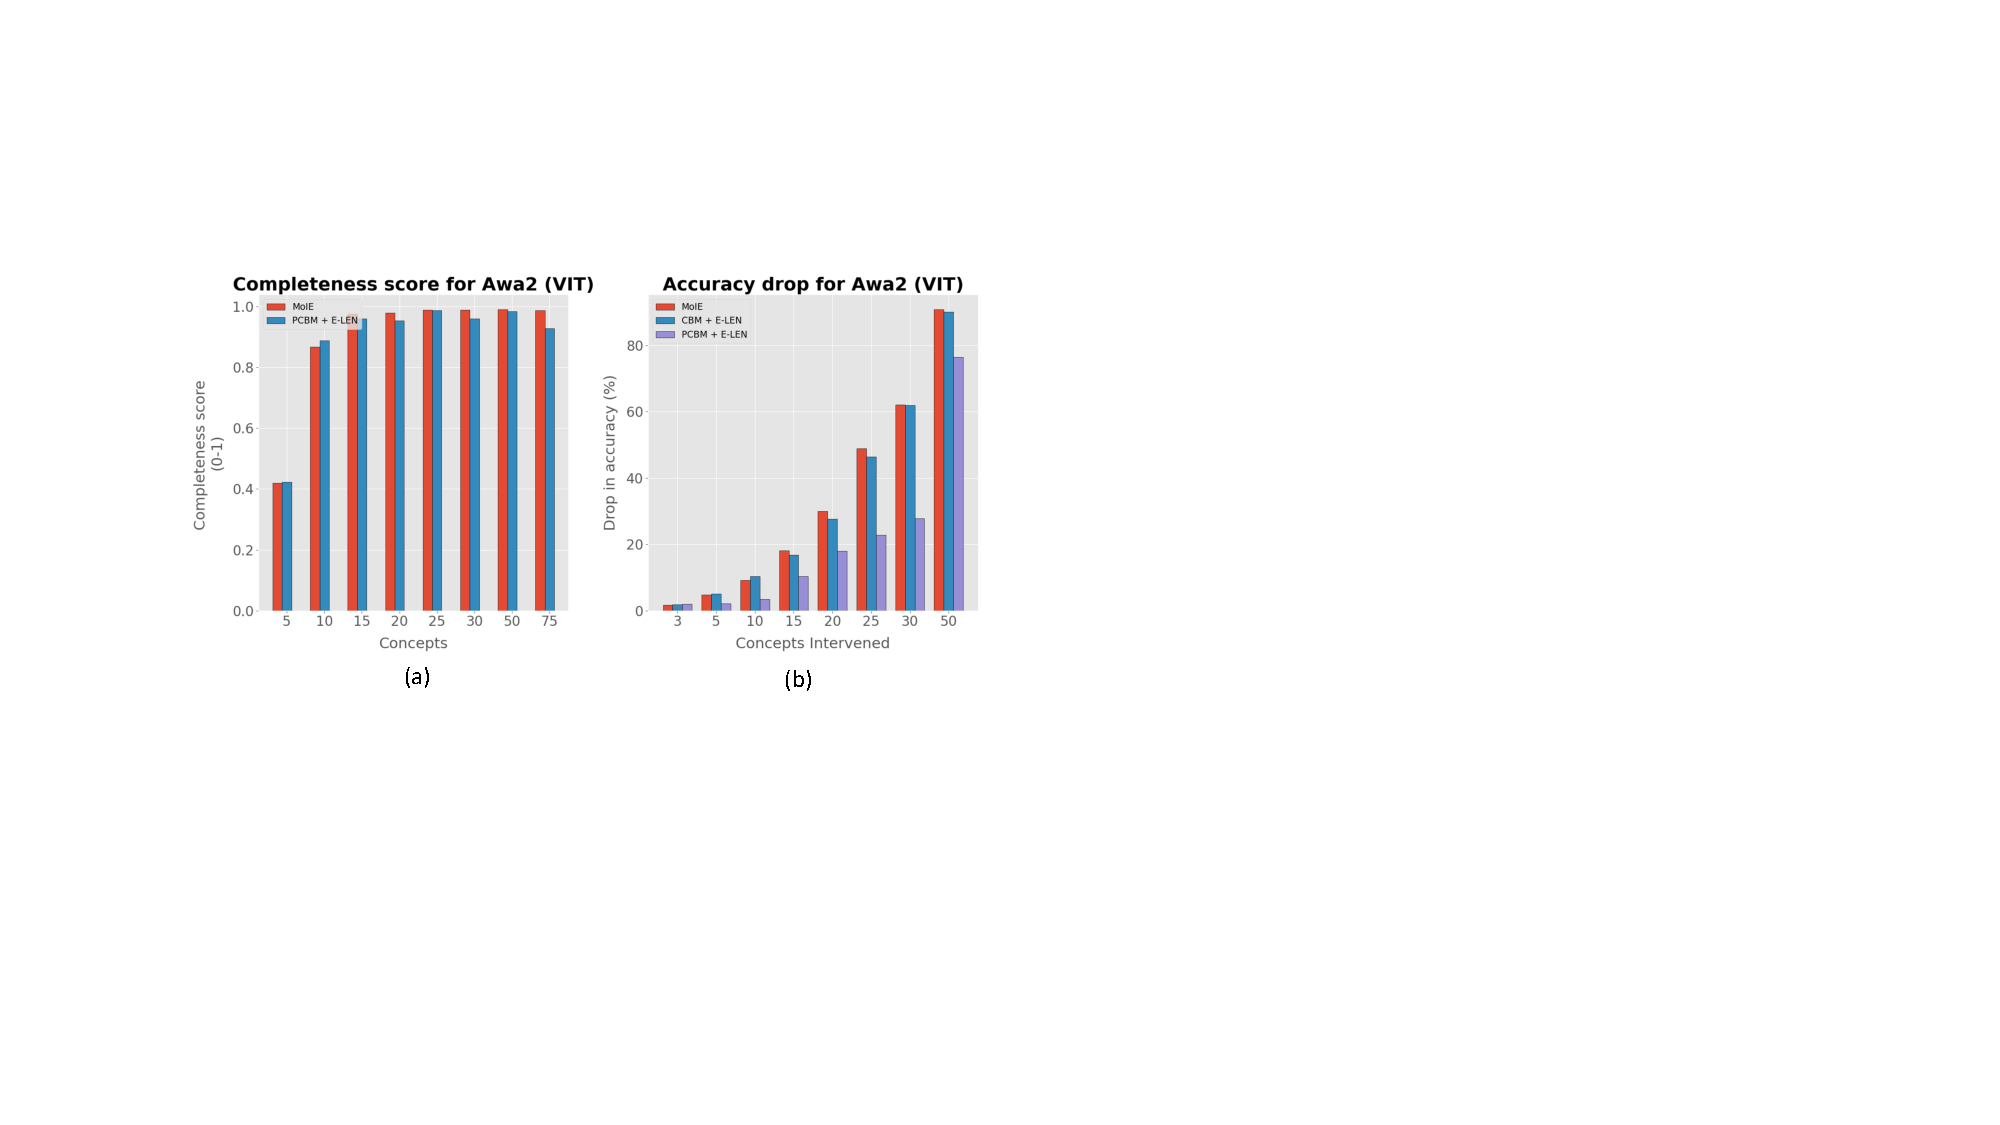
\includegraphics[width=\columnwidth]
{figures/Supp/Awa2.pdf}
\vskip -7pt
\caption{\textbf{(a)} Completeness scores for different significant concepts of Awa2.  \textbf{(b)} Drop in accuracy by zeroing out the concepts for Awa2.}
\vskip -10pt
\label{fig:completeness_acc_awa2}
\end{figure}

\cref{fig:completeness_acc_awa2} shows the completeness scores and the drop in accuracy by zeroing out the concepts for Awa2.

% \subsubsection{Performance drop for MoIE and baselines}
% \label{app:performance_drop_other}
% \begin{figure}
\centering
% \includegraphics[width=1\linewidth]
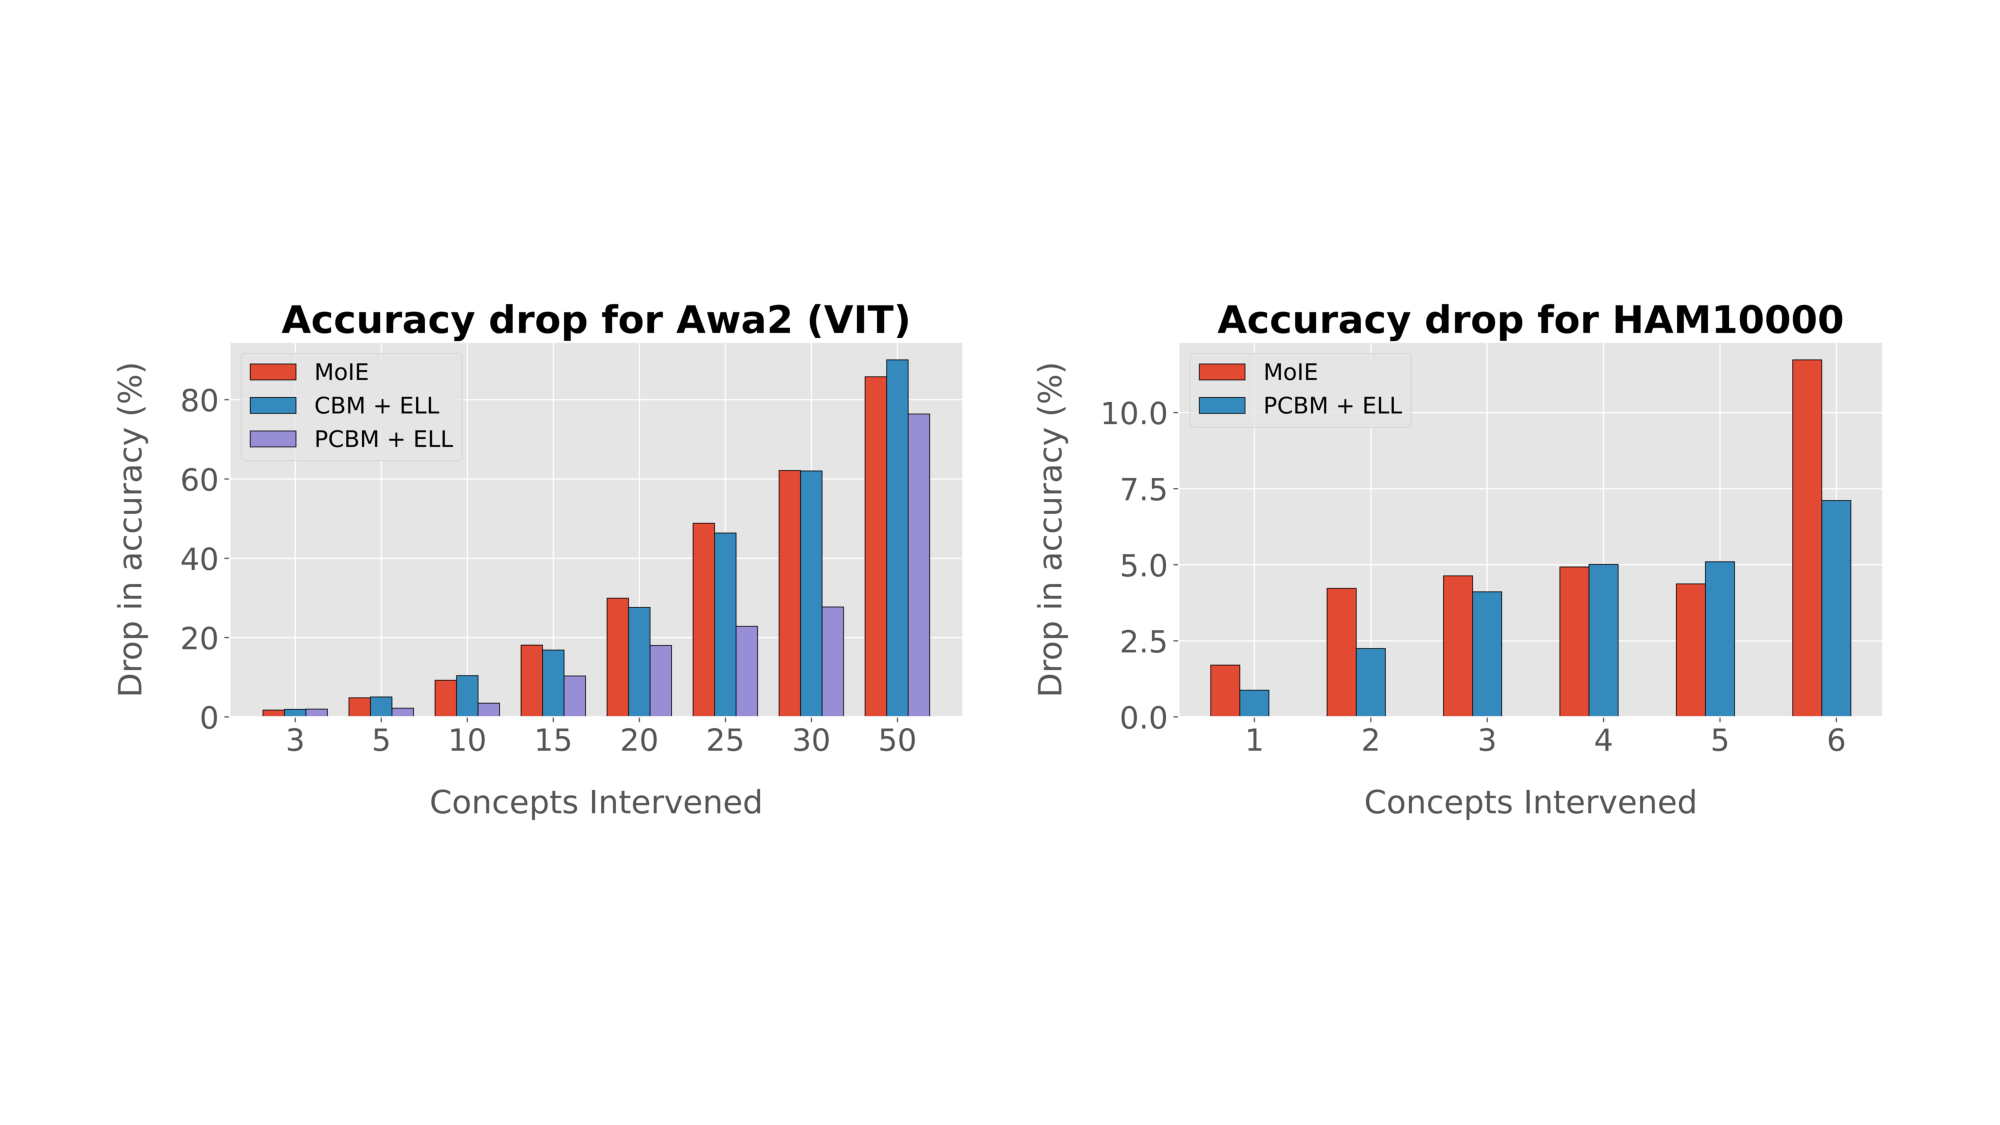
\includegraphics[width=\columnwidth]
{figures/Supp/Acc_drop_ham_awa2.pdf}
\vskip -7pt
\caption{Validation of the concepts utilized for Awa2 (left) and HAM10000 (right) datasets by Inception and VIT-derived MoIE and the baselines respectively.}
\vskip -10pt
\label{fig:valid_concepts_other}
\end{figure}

\cref{fig:valid_concepts_other} shows the performance drop for HAM10000 and Awa2 when we intervene and set the values of the important concepts as zeros.

% \subsubsection{Test time interventions for ResNet models and Awa2}
% \label{app:tti}
% \begin{figure}
\centering
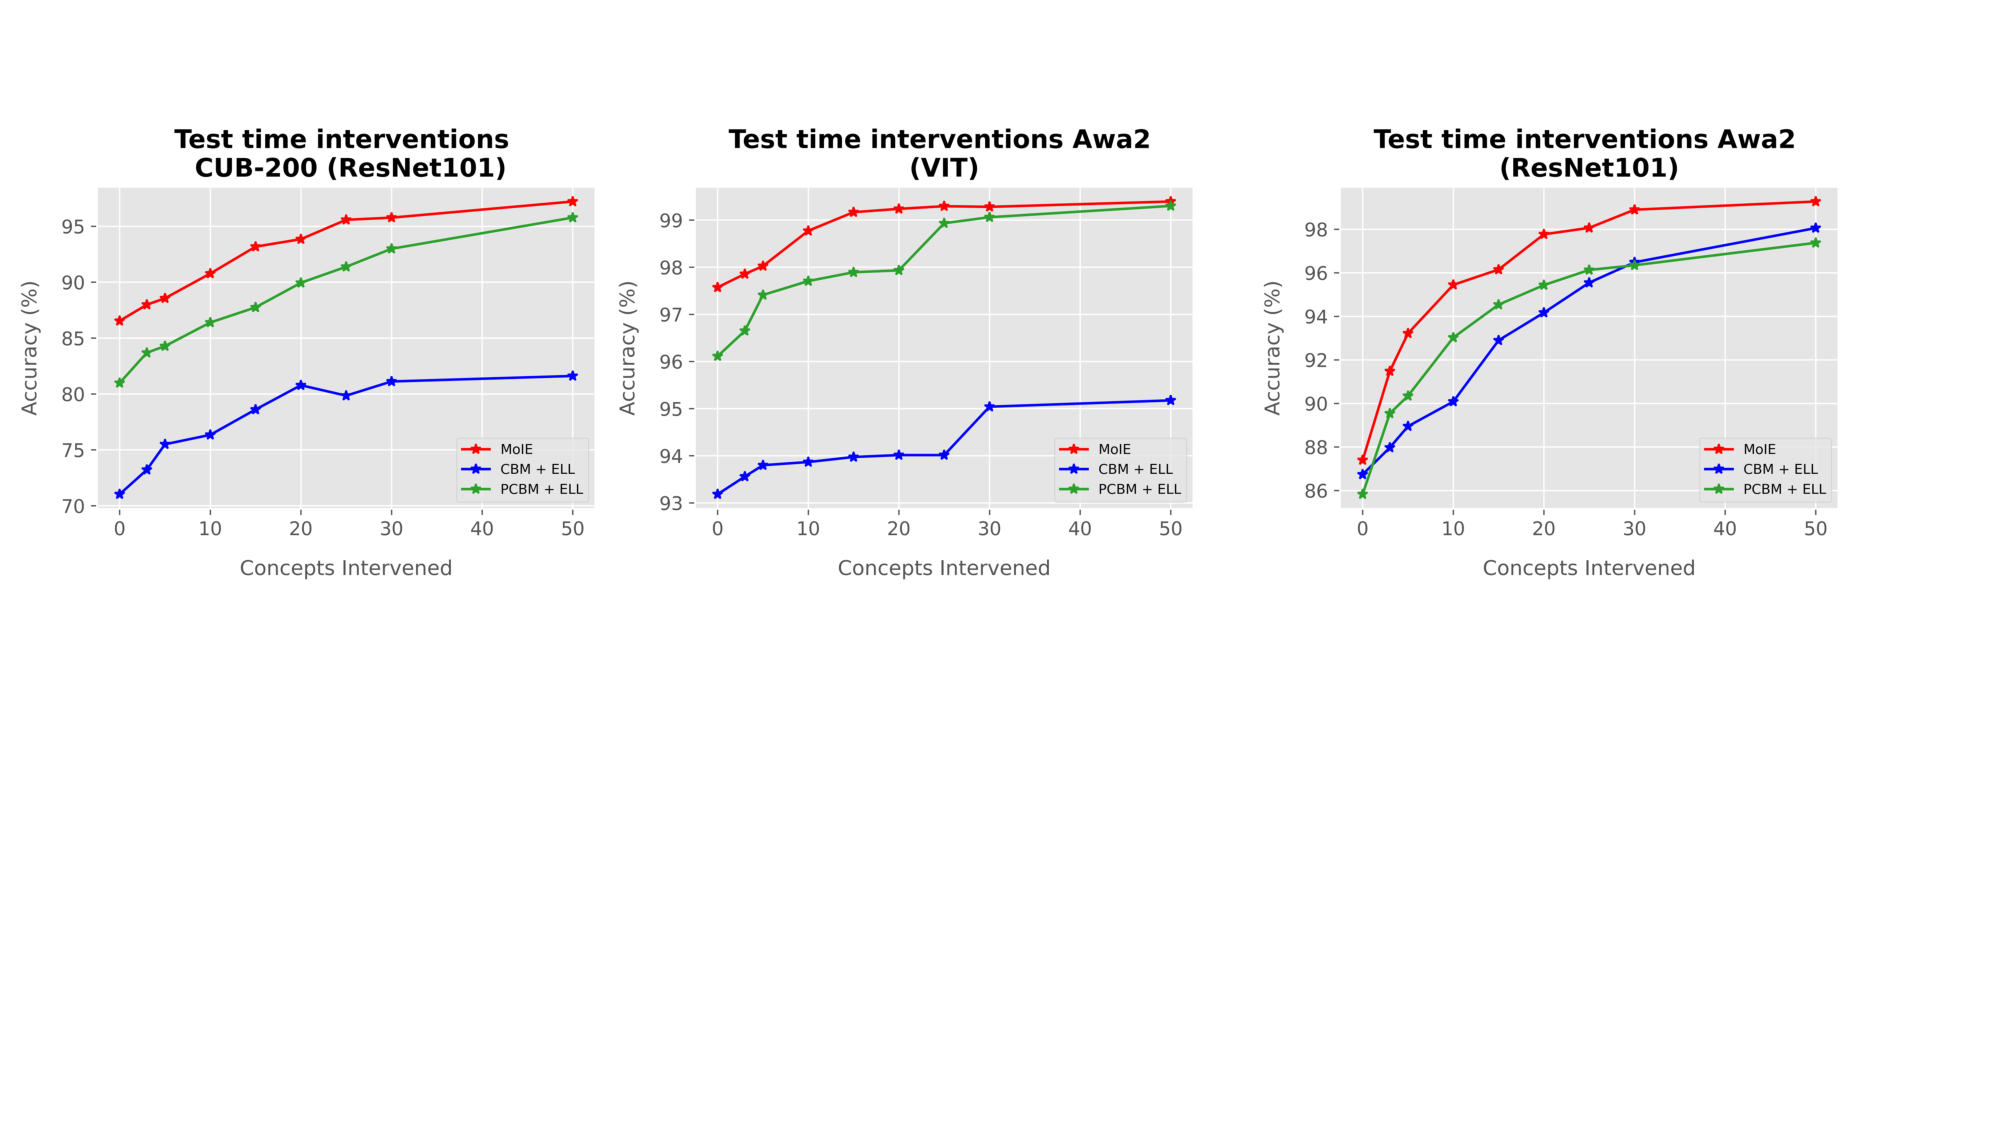
\includegraphics[width=\columnwidth]{figures/Supp/TTI_rest.pdf}
\vskip -7pt
\caption{Illustration of test time interventions for ResNet101-derived models for CUB-200 (left) and VIT-derived models for Awa2 (middle) and ResNet101-driven models for Awa2 (right).}
\vskip -7pt
\label{fig:tti_expert}
\end{figure}

Figure~\ref{fig:tti_expert} shows the results of test time concept interventions for ResNet101-derived models for CUB-200 (left) and VIT-derived models for Awa2 (middle) and ResNet101-driven models for Awa2 (right).

% \subsubsection{Validating concepts by zer}
% \label{app:validate_concepts}
% To validate the concepts using the extracted FOL explanations, we intervene on the concepts in the derived FOL by setting the values of those concepts to zero for each sample. For example, the FOL explanation of instances in expert4 for the class ``Bay Breasted Warbler'' include concepts \st \emph{back\_pattern\_stripped} and \emph{leg\_color\_grey} in~\cref{fig:local_ex_cub}. For intervention, we set the values of these concepts to zero while values of other concepts remain unchanged. Next we pass the complete intervened concept vector as input to the associated expert, compute the
  performance and summarize the results in~\cref{tab:cf_table}. We discover that MoIE is highly susceptible to such interventions, and its performance drops significantly. For example,
  the performance of MoIE deteriorates from 0.91 to 0.42 \% (a 53.8 \% drop) for CUB-200 VIT-derived MoIE. 
  We compare the results with 1) the CBM + ELL baseline corresponding to CUB-200 (both Resnet101 and VIT), Awa2 (both Resnet101 and VIT) and Effusion of MIMIC-CXR; 2) PCBM + ELL baseline for the skin datasets. For CUB-200 VIT-based baseline model, the performance of the baseline drops by 26.5 \% drop, from 0.90 to 0.66. We observe a similar trend for other datasets as well. As MoIE selects more concrete, instance specific concepts than the baseline by covering subsets of data using various experts, its performance degrades severely compared to the baseline. 
  
\begin{table*}[h]
\caption{Validating the concepts purely by extracted FOL rules from MoIE and the baselines. Performance using original explanation refers to the performance of the model employing the concepts from the FOL explanations per sample. We intervene with these concepts by setting their values to zero and reporting it as ``Performance using intervened explanation'' in the table. In addition, we also show the drop in performance for the two scenarios. The larger drop in performance illustrates the model to be more sensitive to such intervention of the derived concepts.}\smallskip
\fontsize{6.75pt}{0.30cm}
\selectfont
\centering
\begin{tabular}{p{2.7em} c c c c c c c}
\toprule 
        \textbf{Model} & \multicolumn{7}{c}{\textbf{Performance using original explanation $\longrightarrow$ Performance using intervened explanation (drop \% )}} \\
       & CUB-200 (ResNet101) & CUB-200 (VIT )& Awa2 (ResNet101) & Awa2 (VIT) & HAM 10000 & ISIC  
       & Effusion\\
\midrule 
    MoIE & 
        0.88 $\rightarrow$ 0.65 (\textbf{26.1}) & 
        0.91 $\rightarrow$ 0.42 (\textbf{53.8}) & 
        0.87 $\rightarrow$ 0.54 (\textbf{37.9}) & 
        0.97 $\rightarrow$ 0.90 (\textbf{7.2})  & 
        0.95 $\rightarrow$ 0.92 (\textbf{3.1})  & 
        0.82 $\rightarrow$ 0.79 (\textbf{3.6})  &
        0.87 $\rightarrow$ 0.82 (\textbf{5.7}) 
    \\
\midrule 
    Baseline & 
        0.71 $\rightarrow$ 0.56 (\textbf{21.1}) & 
        0.90 $\rightarrow$ 0.66 (\textbf{26.5}) & 
        0.86 $\rightarrow$ 0.56 (\textbf{34.8}) & 
        0.94 $\rightarrow$ 0.92 (\textbf{2.1}) & 
        0.94 $\rightarrow$ 0.92 (\textbf{2.1}) &
        0.83 $\rightarrow$ 0.80 (\textbf{3.6}) &
        0.73 $\rightarrow$ 0.72 (\textbf{1.3})
        \\
\bottomrule
\end{tabular}
\label{tab:cf_table}
\end{table*}

\subsubsection{Example of expert-specific test time intervention}
\label{app:tti_qual}
\begin{figure}[h]
\centering
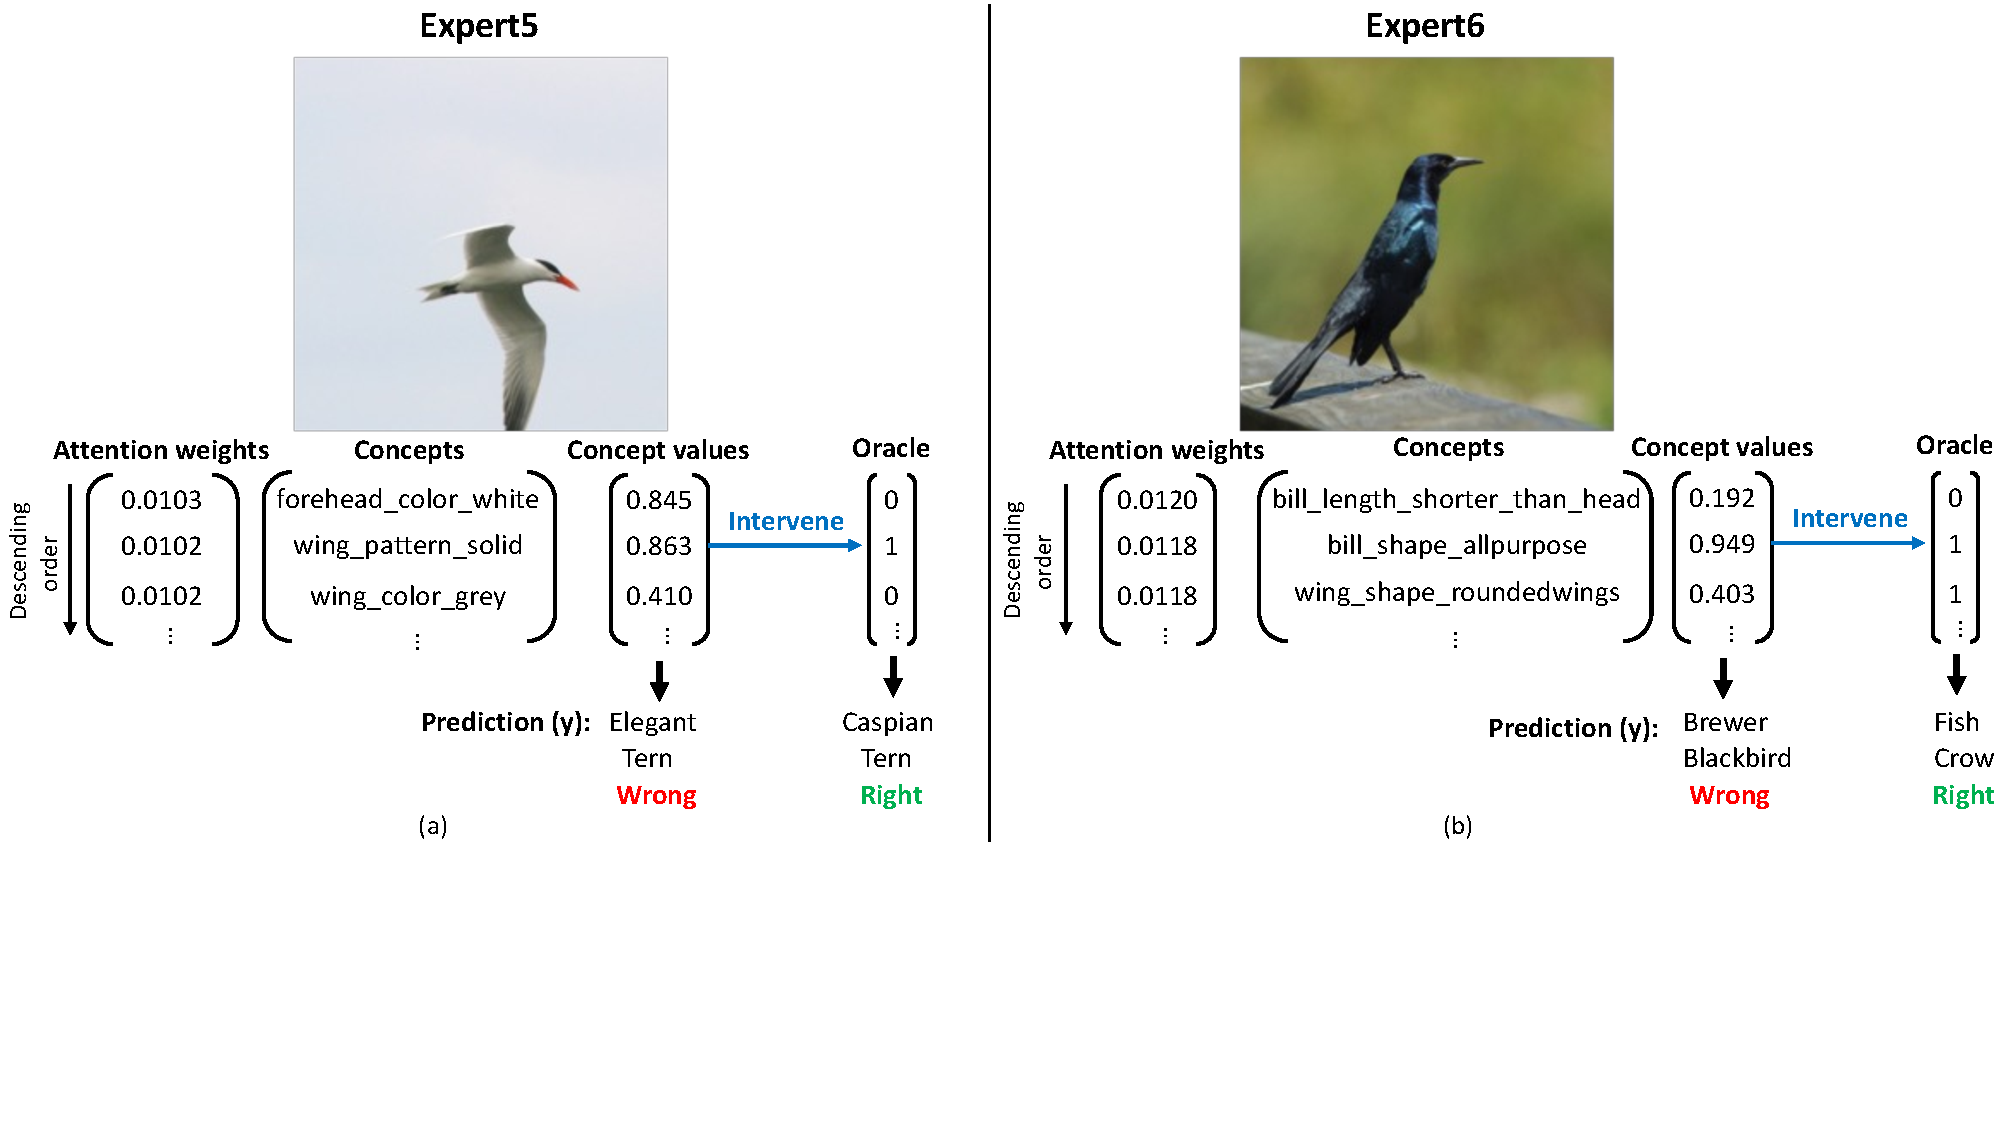
\includegraphics[width=1 \linewidth]{figures/Supp/TTI_qual.pdf}
\caption{Illustration of test time intervention of top-3 concepts for ``harder'' samples identified by the last two experts of VIT-driven MoIE. We adopt E-LEN~\cite{barbiero2022entropy} as the experts. Thus, each concept is associated with an attention weight after training, signifying its prediction importance. So, here we intervene the top 3 concepts with the highest attention weights for samples routed to expert 5 (\textbf{\emph{left}}) and expert 6 (\textbf{\emph{right}}). These samples are considered the ``harder'' samples as they are routed to the last two experts of MoIE. We demonstrate that the test time intervention corrects the prediction. }
\label{fig:tti_qual}
\vspace{-2.5pt}
\end{figure}
~\cref{fig:tti_qual} demonstrates an example of test time intervention of concepts for ``harder'' samples identified by the last two experts of VIT-driven MoIE.

\subsubsection{Diversity of explanations for CUB}
\label{app:local_cub}
\begin{figure}[t]
\centering
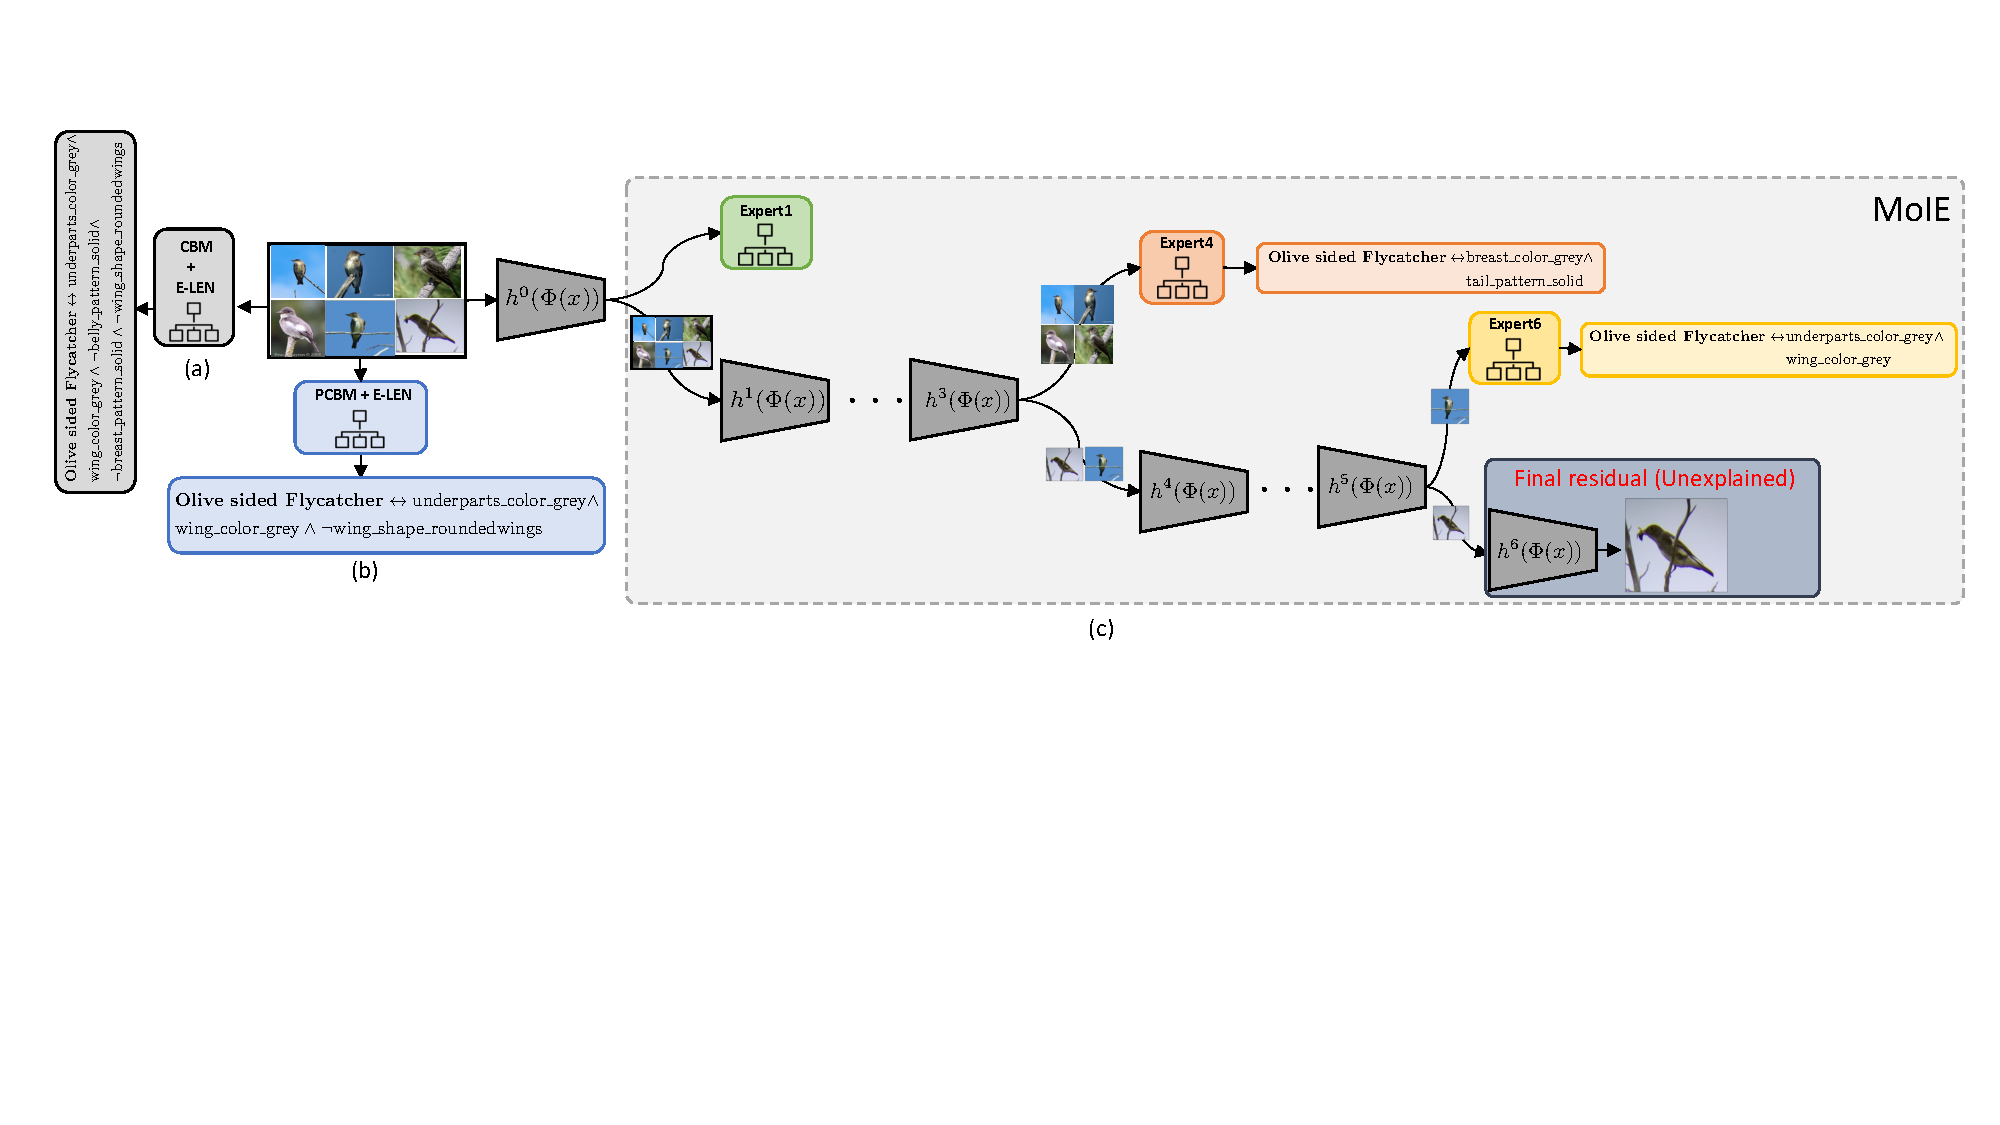
\includegraphics[width=1 \linewidth]{figures/Supp/Olive_sided.pdf}
\vspace{-10pt}
\caption{Construction logical explanations of the samples of a category, ``Olive sided Flycatcher'' in the CUB-200 dataset for (a) VIT-based sequential CBM + E-LEN as an \emph{interpretable by design} baseline, (b) VIT-based PCBM + E-LEN as a posthoc based baseline, (c) various experts in MoIE at inference. This is an example where the final residual covers the unexplained sample, which is ``harder'' to explain (indicated in \emph{red}). Also, MoIE can capture more instance-specific concepts than generic ones by the baselines.}
\label{fig:local_ex_cub_olive_sided}
\vspace{-2.5pt}
\end{figure}


\begin{figure}[h]
\centering
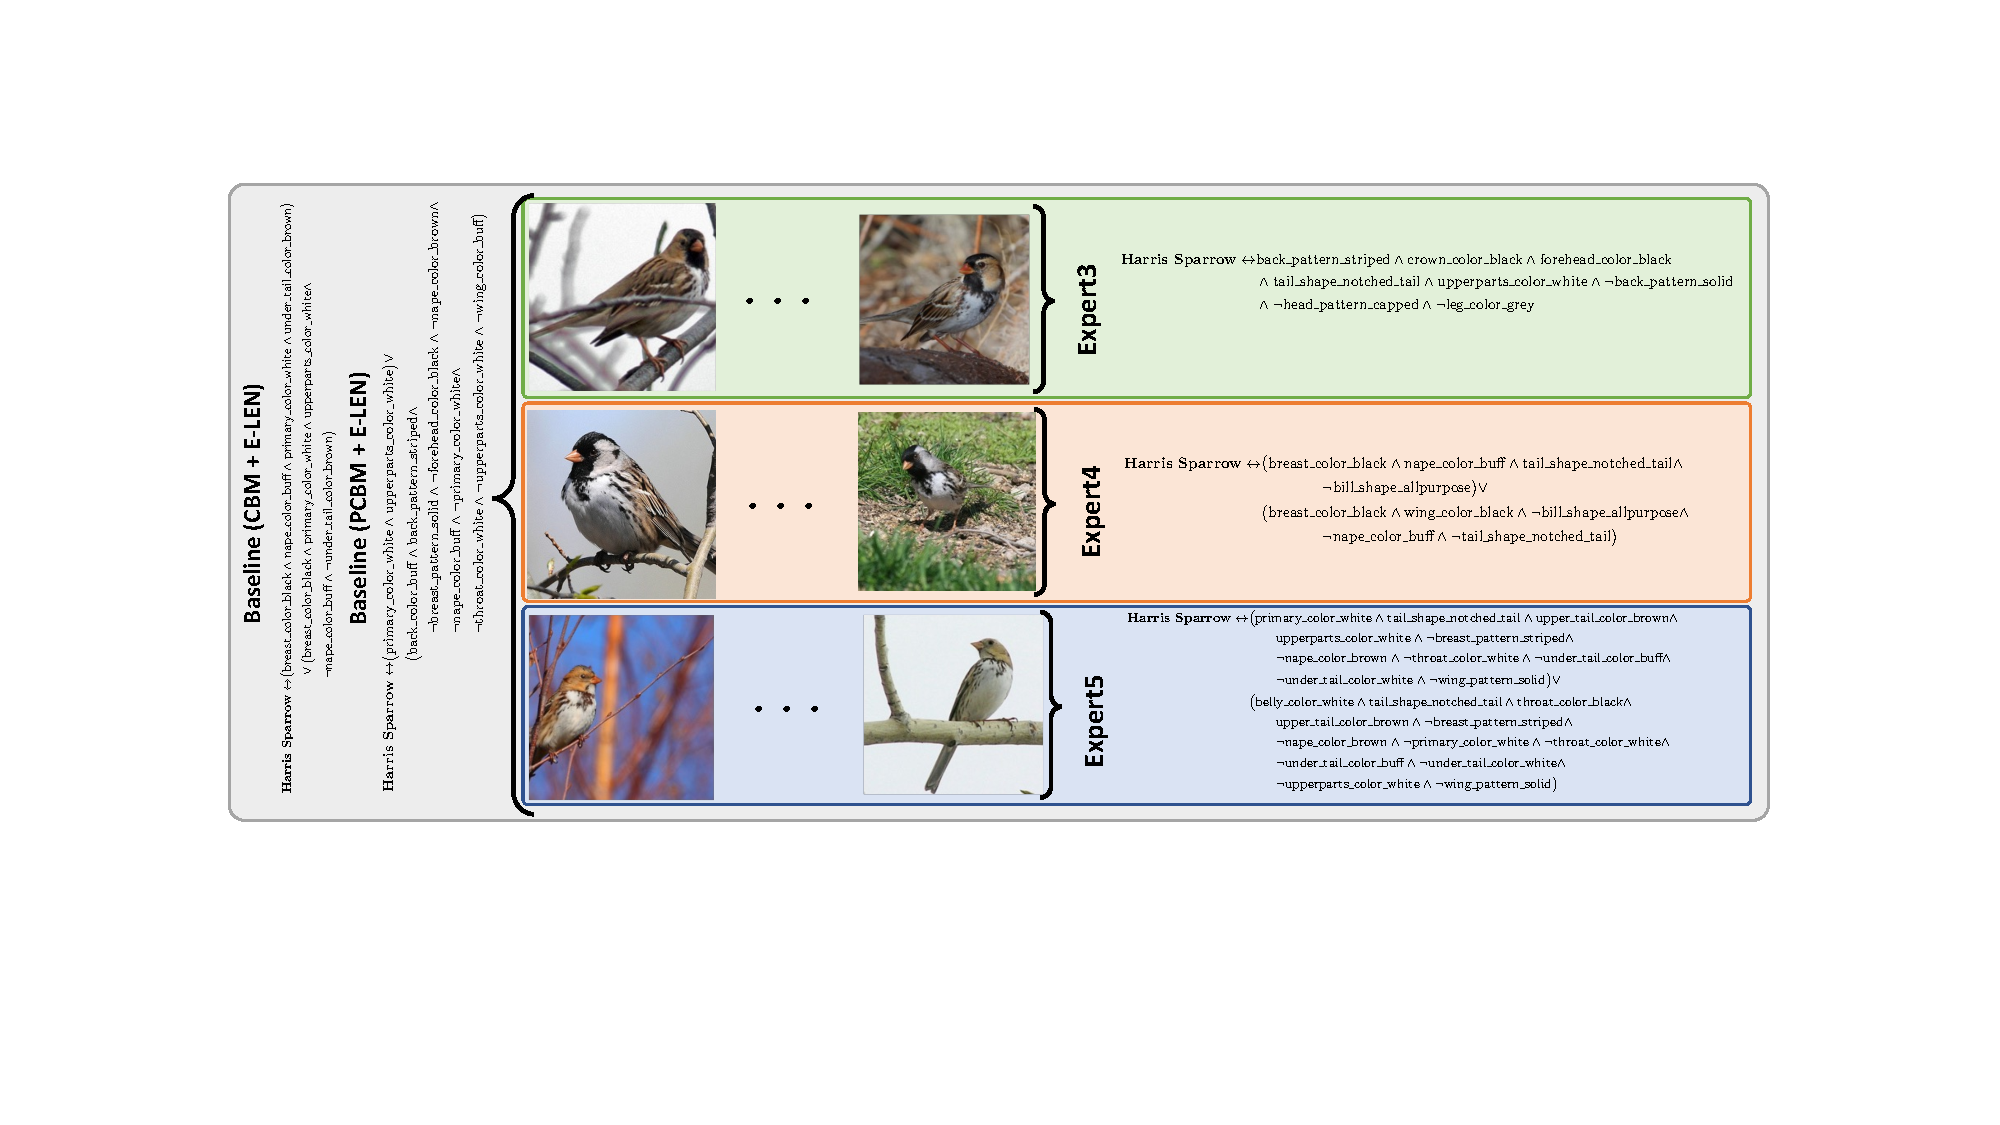
\includegraphics[width=1 \linewidth]{figures/Supp/Harris_sparrow.pdf}
\vspace{-10pt}
\caption{Construction logical explanations of the samples of a category, ``Harris Sparrow'' in the CUB-200 dataset for (a) VIT-based sequential CBM + E-LEN as an \emph{interpretable by design} baseline, (b) VIT-based PCBM + E-LEN as a posthoc based baseline, (c) various experts in MoIE at inference.}
\label{fig:local_ex_cub_harris}
\vspace{-2.5pt}
\end{figure}

\begin{figure}[h]
\centering
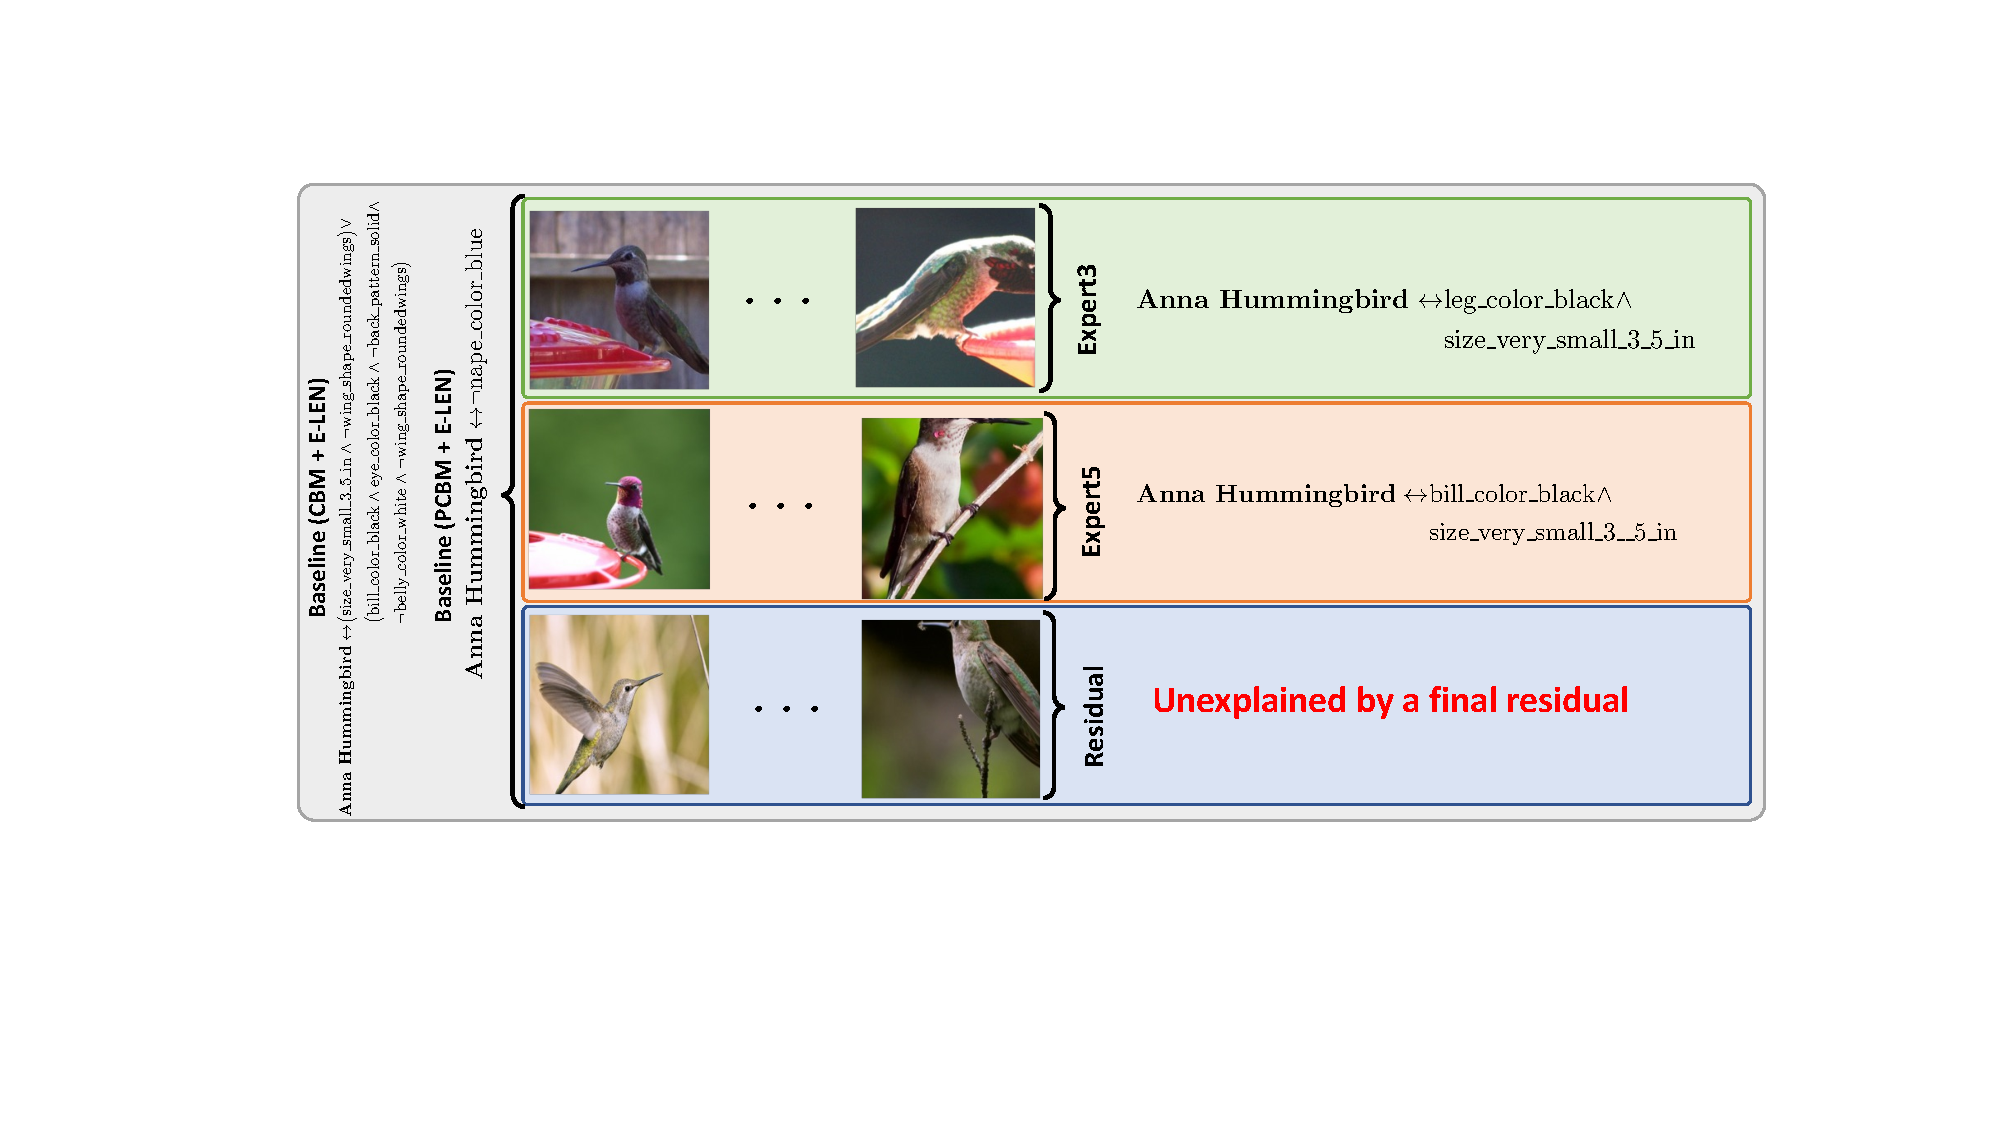
\includegraphics[width=1 \linewidth]{figures/Supp/Anna_hummingbird.pdf}
\vspace{-10pt}
\caption{Construction logical explanations of the samples of a category, ``Anna Hummingbird'' in the CUB-200 dataset for (a) VIT-based sequential CBM + E-LEN as an \emph{interpretable by design} baseline, (b) VIT-based PCBM + E-LEN as a posthoc based baseline, (c) various experts in MoIE at inference.}
\label{fig:local_ex_anna}
\vspace{-2.5pt}
\end{figure}

\begin{figure}[h]
\centering
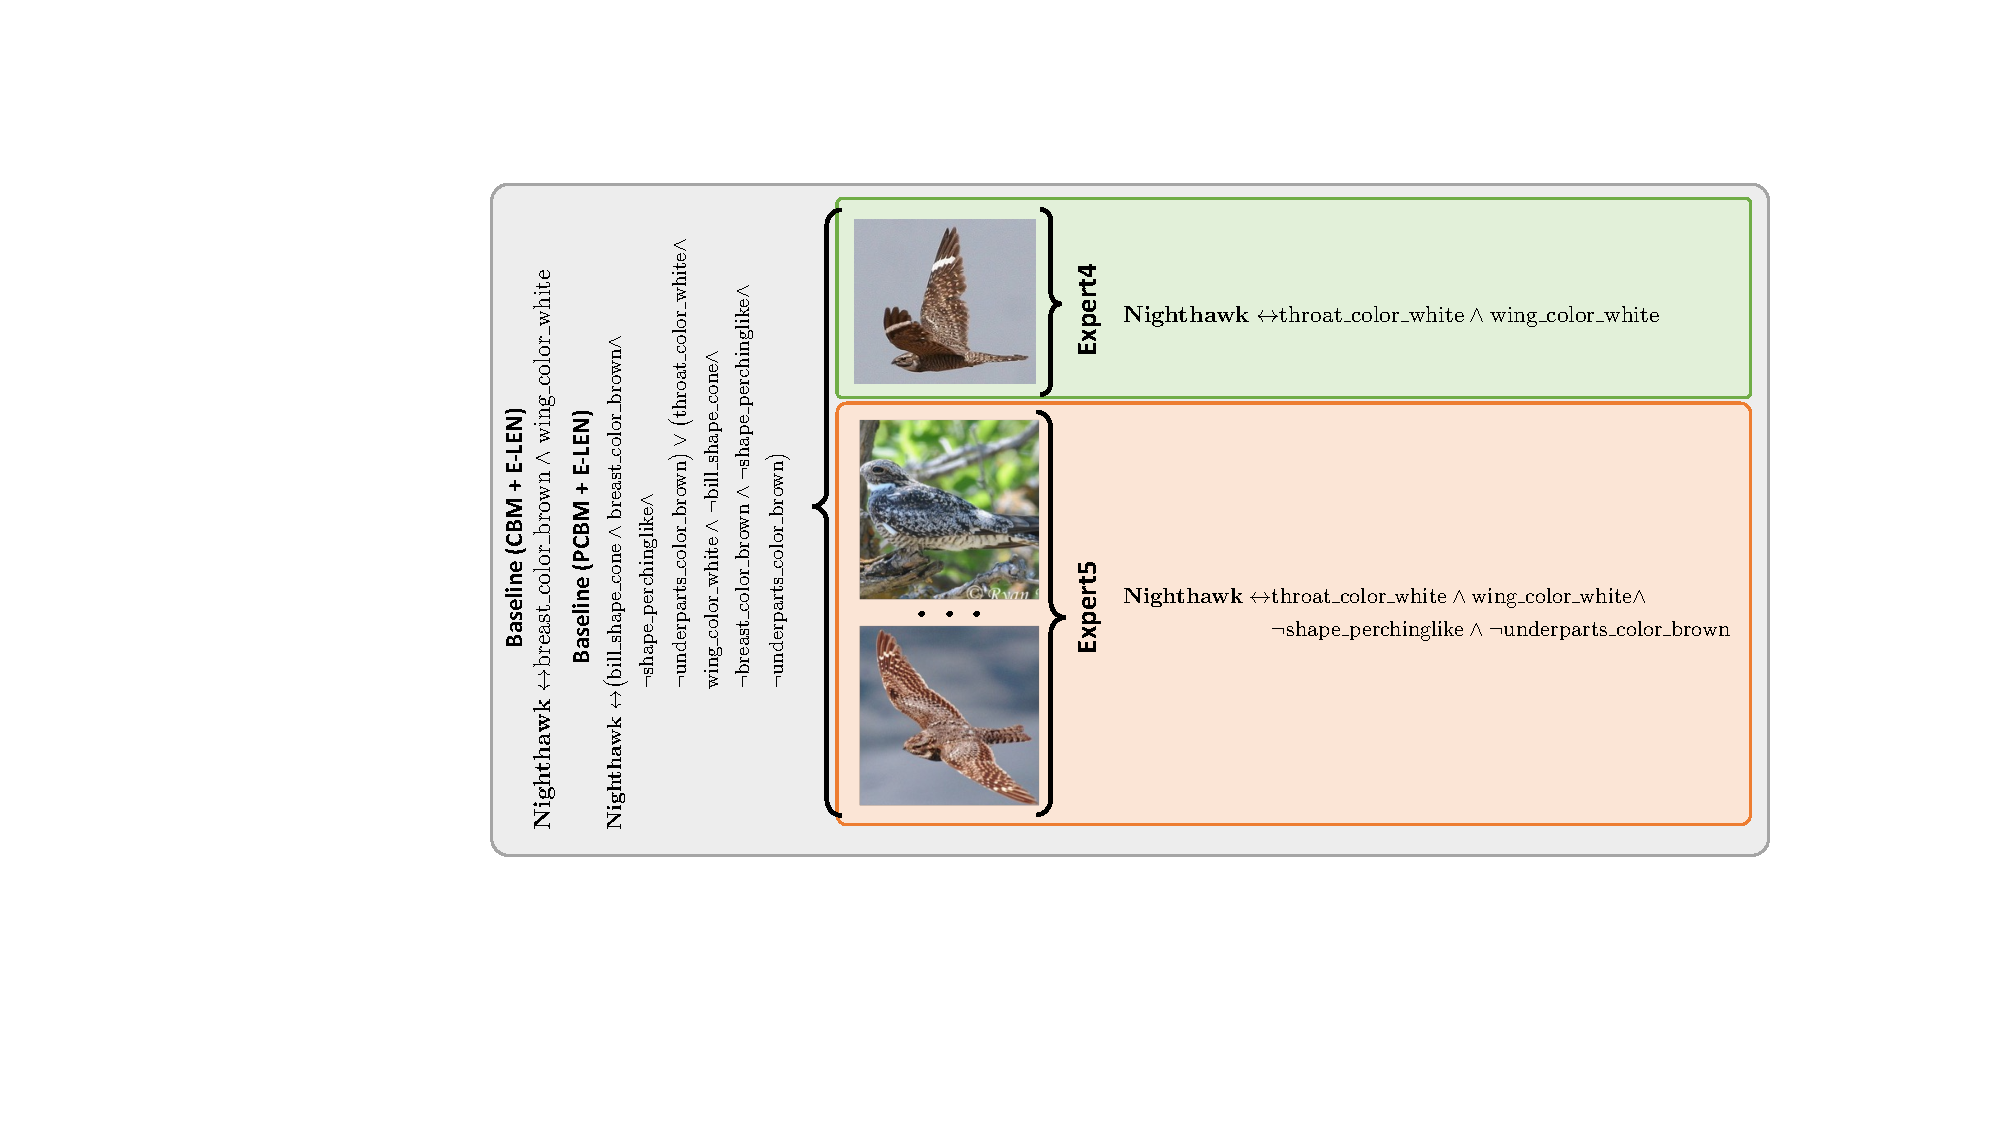
\includegraphics[width=1 \linewidth]{figures/Supp/Nighthawk.pdf}
\vspace{-10pt}
\caption{Construction logical explanations of the samples of a category, ``Nighthawk'' in the CUB-200 dataset for (a) VIT-based sequential CBM + E-LEN as an \emph{interpretable by design} baseline, (b) VIT-based PCBM + E-LEN as a posthoc based baseline, (c) various experts in MoIE at inference. }
\label{fig:local_ex_nighthawk}
\vspace{-2.5pt}
\end{figure}

\begin{figure}[h]
\centering
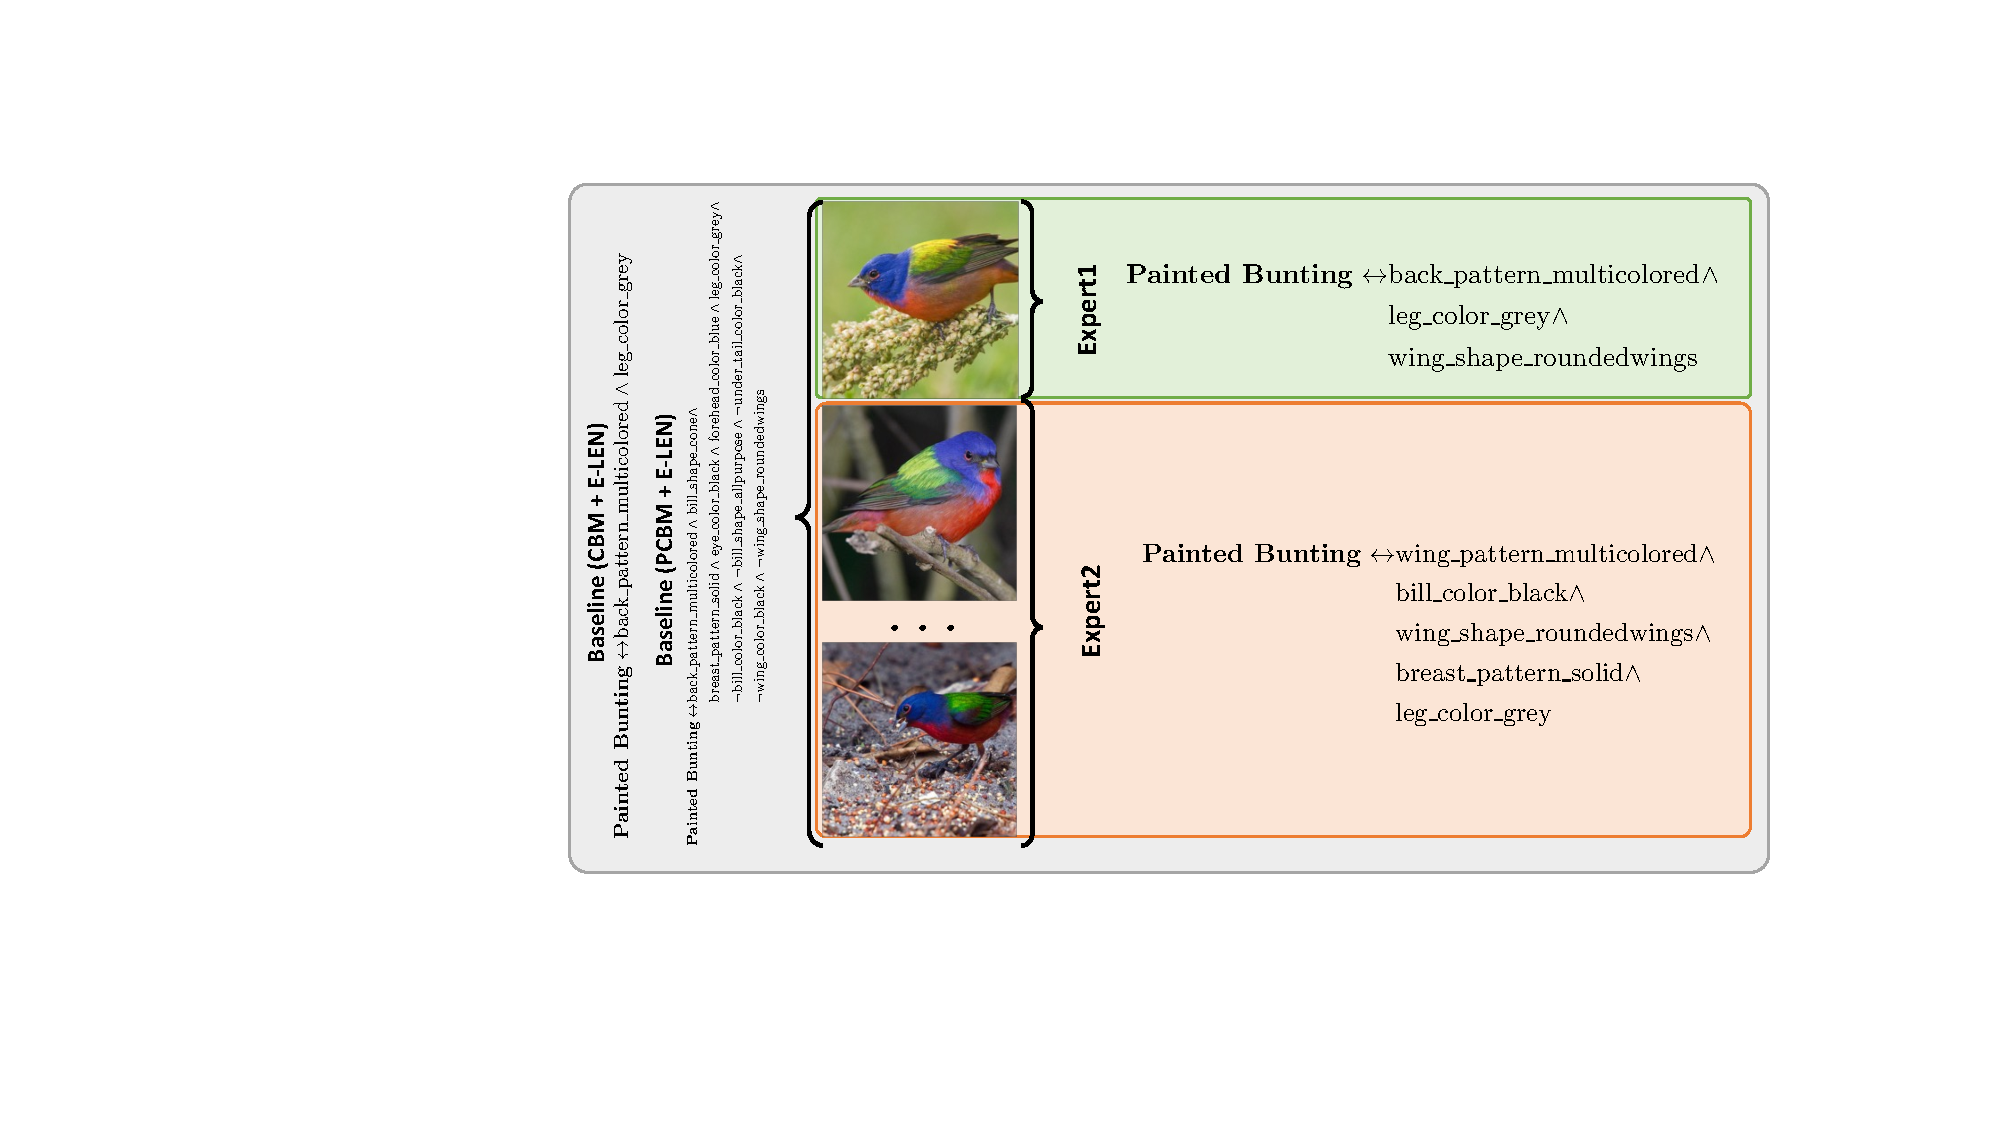
\includegraphics[width=1 \linewidth]{figures/Supp/Painted_bunting.pdf}
\vspace{-10pt}
\caption{Construction logical explanations of the samples of a category, ``Painted Bunting'' in the CUB-200 dataset for (a) VIT-based sequential CBM + E-LEN as an \emph{interpretable by design} baseline, (b) VIT-based PCBM + E-LEN as a posthoc based baseline, (c) various experts in MoIE at inference. }
\label{fig:local_ex_cub_painted}
\vspace{-2.5pt}
\end{figure}

\cref{fig:local_ex_cub_olive_sided} shows the construction of instance-specific local FOL explanations of a category, ``Olive sided Flycatcher'' in the CUB-200 dataset for the VIT-based baselines and MoIE. In this example, the final expert6 covers the relatively ``harder'' sample.~\cref{fig:local_ex_cub_harris},~\cref{fig:local_ex_anna},~\cref{fig:local_ex_nighthawk},~\cref{fig:local_ex_cub_painted} shows more such FOL explanations. All these examples demonstrate MoIE's high capability to identify more meaningful instance-specific concepts in FOL explanations. In contrast, the baselines identify the generic concepts for all samples in a class.






\subsubsection{Diversity of explanations for Awa2}
\label{app:local_awa2}
\begin{figure*}[h]
\centering
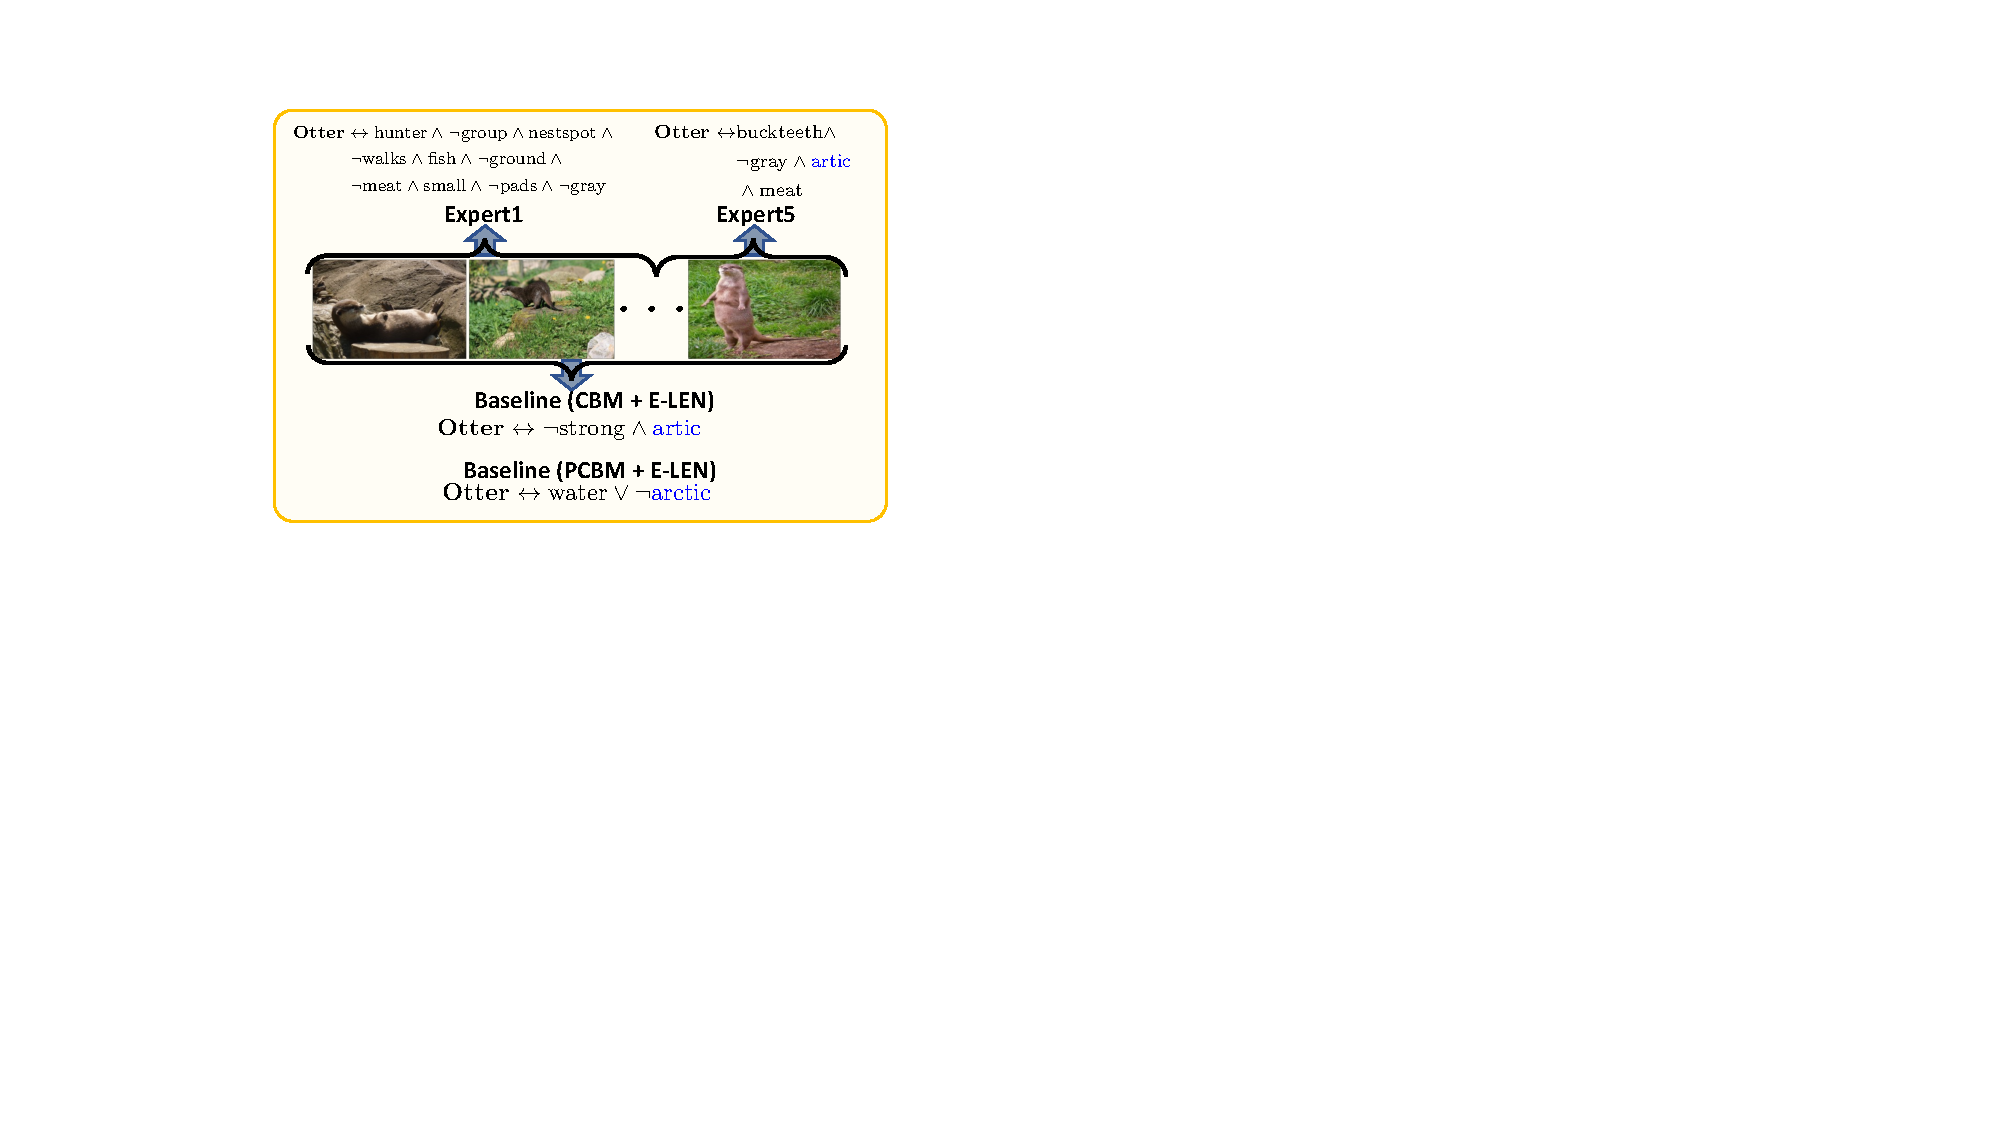
\includegraphics[width=\columnwidth]{figures/Supp/Local_awa2_otter.pdf}
\vspace{-10pt}
\caption{Flexibility of FOL explanations by VIT-derived MoIE  MoIE and the CBM + E-LEN and PCBM + E-LEN baselines for Awa2 dataset to classify ``Otter'' at inference. Both the baseline's FOL constitutes identical concepts to distinguish all the samples. However, expert1 classifies ``Otter'' with \textit{hunter}, \textit{group} \etc as the identifying concept for the instances covered by it. Similarly expert5 classifies ``Otter'' using \textit{buckteeth}, \textit{gray} \etc. Note that, \textit{meat} and \textit{gray}  are shared between the two experts. We highlight the shared concepts (\textit{artic}) between the experts and the baselines as blue.}
\label{fig:local_awa2_otter}
\vspace{-2.5pt}
\end{figure*}

\begin{figure*}[h]
\centering
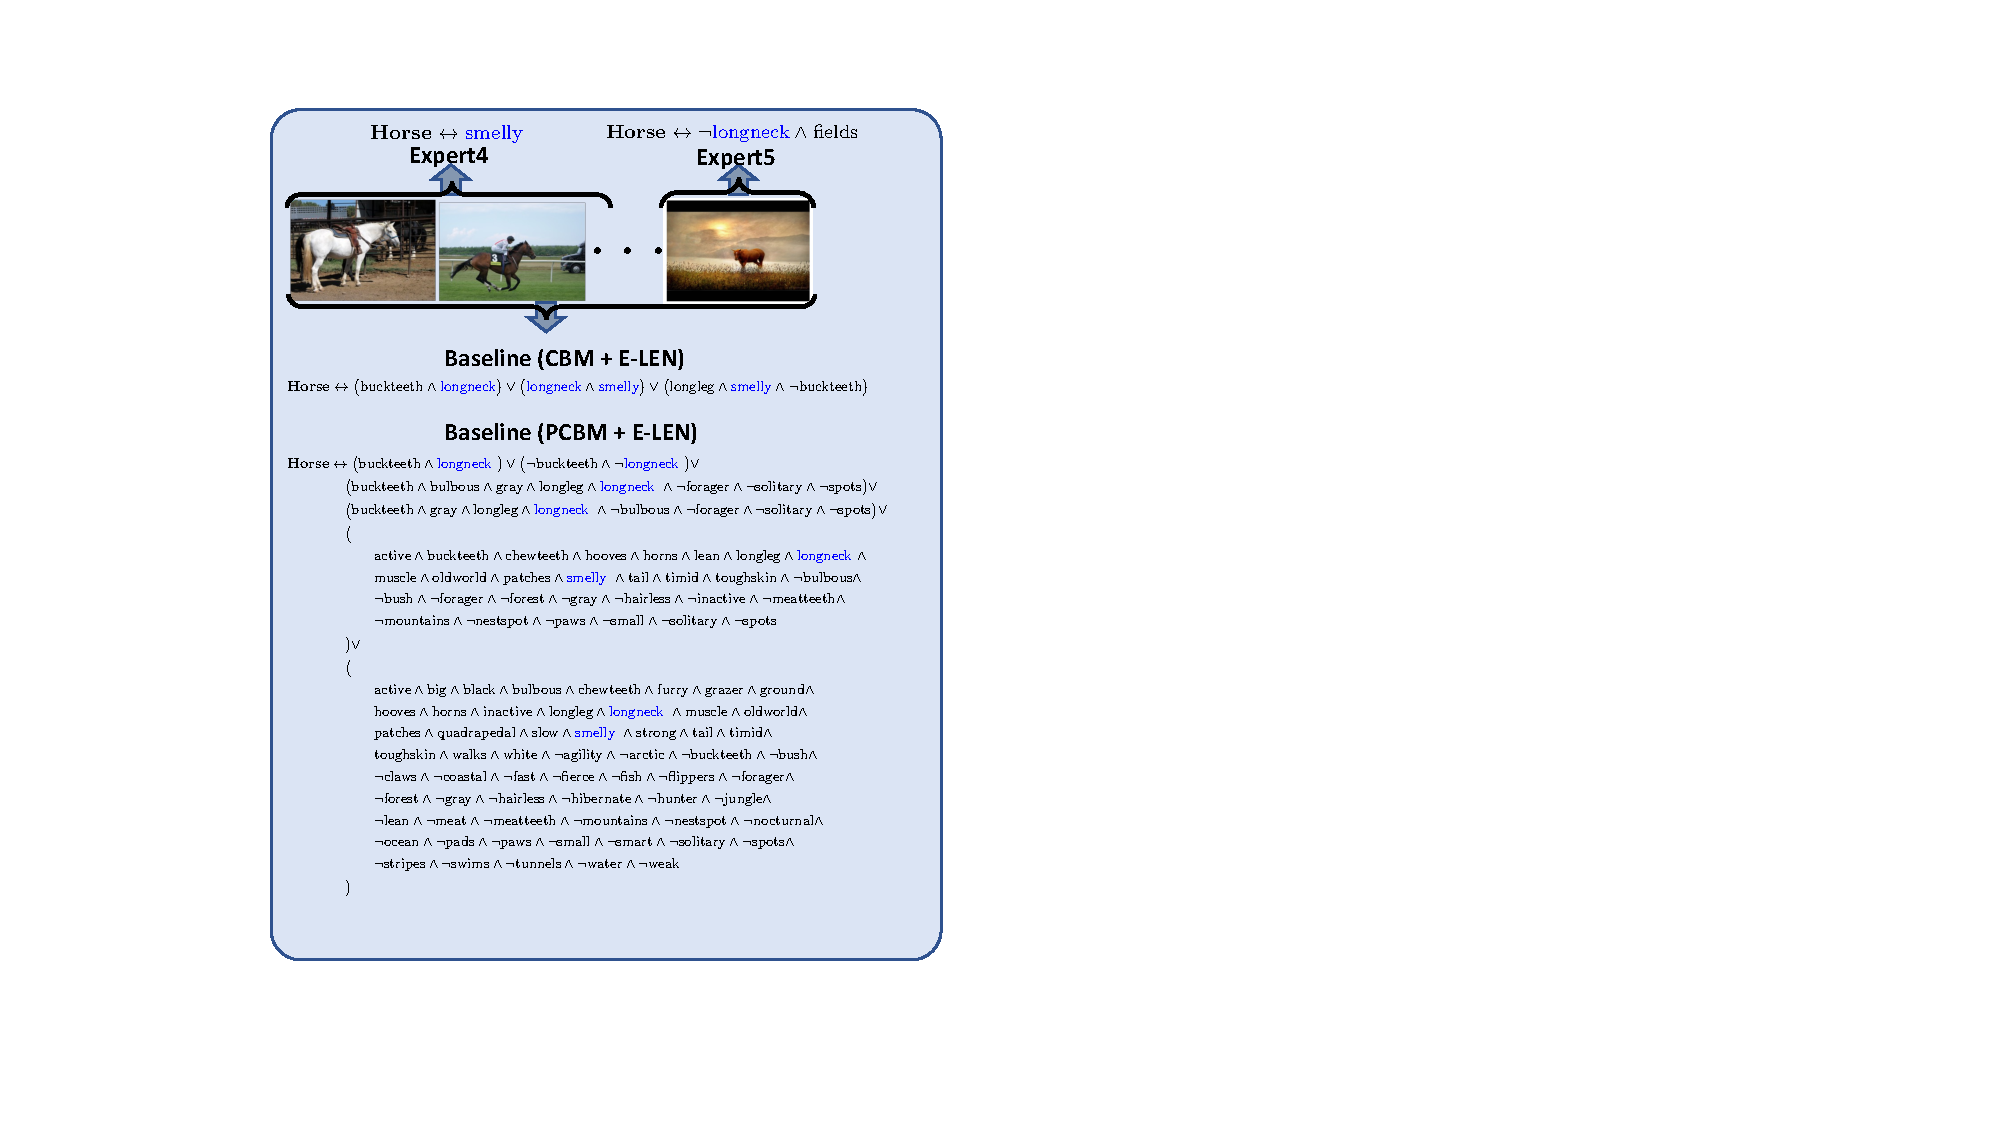
\includegraphics[width=20cm,
  height=20cm,
  keepaspectratio]{figures/Supp/Local_awa2_horse.pdf}
\vspace{-10pt}
\caption{Flexibility of FOL explanations by VIT-derived MoIE  MoIE and the CBM + E-LEN and PCBM + E-LEN baselines for Awa2 dataset to classify ``Horse'' at inference. Both the baseline's FOL constitutes identical concepts to distinguish all the samples. However, expert4 classifies ``Horse'' with \textit{smelly} as the identifying concept for the instances covered by it. Similarly, expert5 classifies the same ``Horse'' using \textit{longneck} and \textit{fields}. We highlight the shared concepts between the experts and the baselines as blue.}
\label{fig:local_awa2_horse}
\vspace{-2.5pt}
\end{figure*}

\cref{fig:local_awa2_otter} and~\ref{fig:local_awa2_horse} demonstrate the flexibility of instance-specific local FOL explanations by VIT-derived MoIE compared to the different baselines for the Awa2 dataset qualitatively.

\subsubsection{VIT-based experts compose of less concepts than the ResNet-based counterparts}
\label{app:comparison_arch}
\begin{figure}[h]
\centering
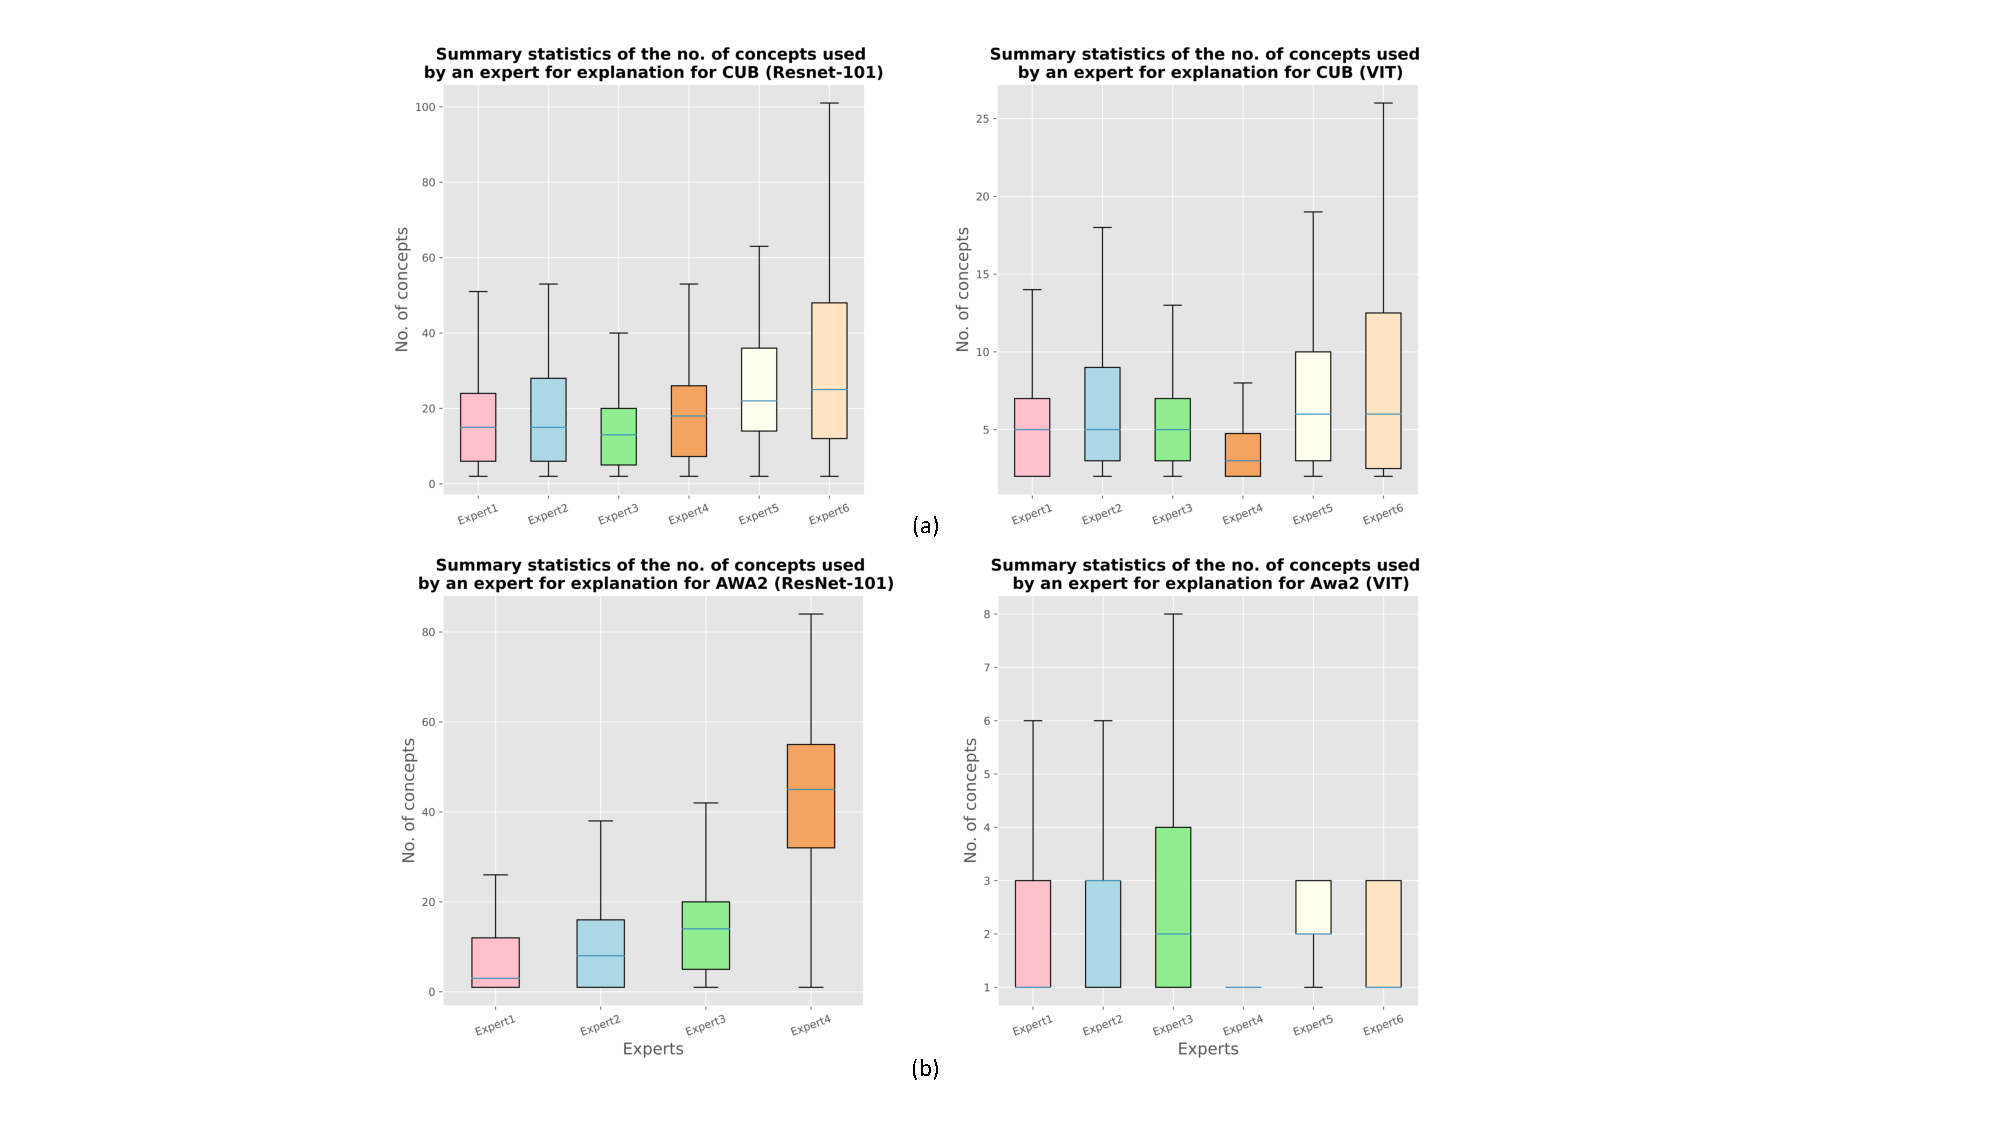
\includegraphics[width=1\textwidth]{figures/Supp/Summary_stats_vit_resnet.pdf}
\caption{Summary statistics of the number of concepts utilized by various experts of datasets (a) CUB -200(top row) and (b) Awa2 (bottom row). In general, we can see that experts carving out the explanations from VIT often uses less number of concepts.}
\label{fig:stats_ex_cub}
\end{figure}



\cref{fig:stats_ex_cub} shows the summary statistics for multiclass classification vision datasets. For both datasets, we observe that the VIT-based MoIE uses fewer concepts for explanation than their ResNet-based counterparts. For example, for the CUB-200 dataset, expert6 of VIT-backbone requires 25 concepts compared to 105 by expert6 of ResNet-101-backbone (~\cref{fig:stats_ex_cub}a). The 105 concepts by expert6 is the highest number of concepts utilized by any expert for CUB-200. Similarly, for Awa2, the highest number concept used by an expert is 8 for the VIT-based backbone compared to 80 for the ResNet-101-based backbone (\cref{fig:stats_ex_cub}b).
As mentioned before, the average number of concepts for class $j$ = $\frac{\sum\text{all concepts for the samples belong to class $j$}}{\text{\# samples of class $j$}}$. We can see that for ResNet-101, on average 80 concepts are required to explain a sample correctly for the class ``Rhinoceros\_Auklet'' (expert3 in~\cref{fig:cnn_cub_concept_3_4} a). However, for VIT, only 6 concepts are needed to explain a sample correctly ``Rhinoceros\_Auklet'' (expert3  in~\cref{fig:vit_cub_concept_3_4} a). From both of these figures, we can see that different experts require a different number of concepts to explain the same class. For example,~\cref{fig:vit_cub_concept_1_2}  (b) and~\cref{fig:vit_cub_concept_5_6} (b) reveal that experts 2 and 6 require 25 and 58 concepts on average to explain ``Artic\_Tern'' correctly respectively for VIT-derived MoIE.


% Figures \ref{fig:vit_cub_concept_1_2}, \ref{fig:vit_cub_concept_3_4} and \ref{fig:vit_cub_concept_5_6} display the average number of concepts required to predict a bird species correctly in the Cub-200 dataset for all the experts of VIT as backbones. Also, Figures \ref{fig:cnn_cub_concept_1_2}, \ref{fig:cnn_cub_concept_3_4} and \ref{fig:cnn_cub_concept_5_6} display the same for the ResNet-101 based counterparts. 
~\cref{fig:Awa2_VIT_a}, ~\cref{fig:Awa2_VIT_b},~\cref{fig:Awa2_VIT_c} display the average number of concepts required to predict an animal species correctly in the Awa2 dataset for VIT as backbones. Similarly~\cref{fig:Awa2_CNN_a} and~\cref{fig:Awa2_CNN_b} display the average number of concepts required to predict an animal species correctly in the Awa2 dataset for ResNet101 as backbones. We can see that for ResNet101, on average, 80 concepts are required to explain a sample correctly for the class ``Weasel'' (Expert1 in~\cref{fig:Awa2_CNN_a} a). However, for VIT, only three concepts are needed to explain a sample correctly for ``Weasel'' (Expert 6 in~\cref{fig:Awa2_VIT_c} f). Also, from both of these figures, we can see that different experts require different number concepts to explain the same class. For example,~\cref {fig:Awa2_VIT_c} (e) and (f) reveal that experts 5 and 6 require 4 and 30 concepts on average to explain ``Wolf'' correctly.

\begin{figure}
\centering
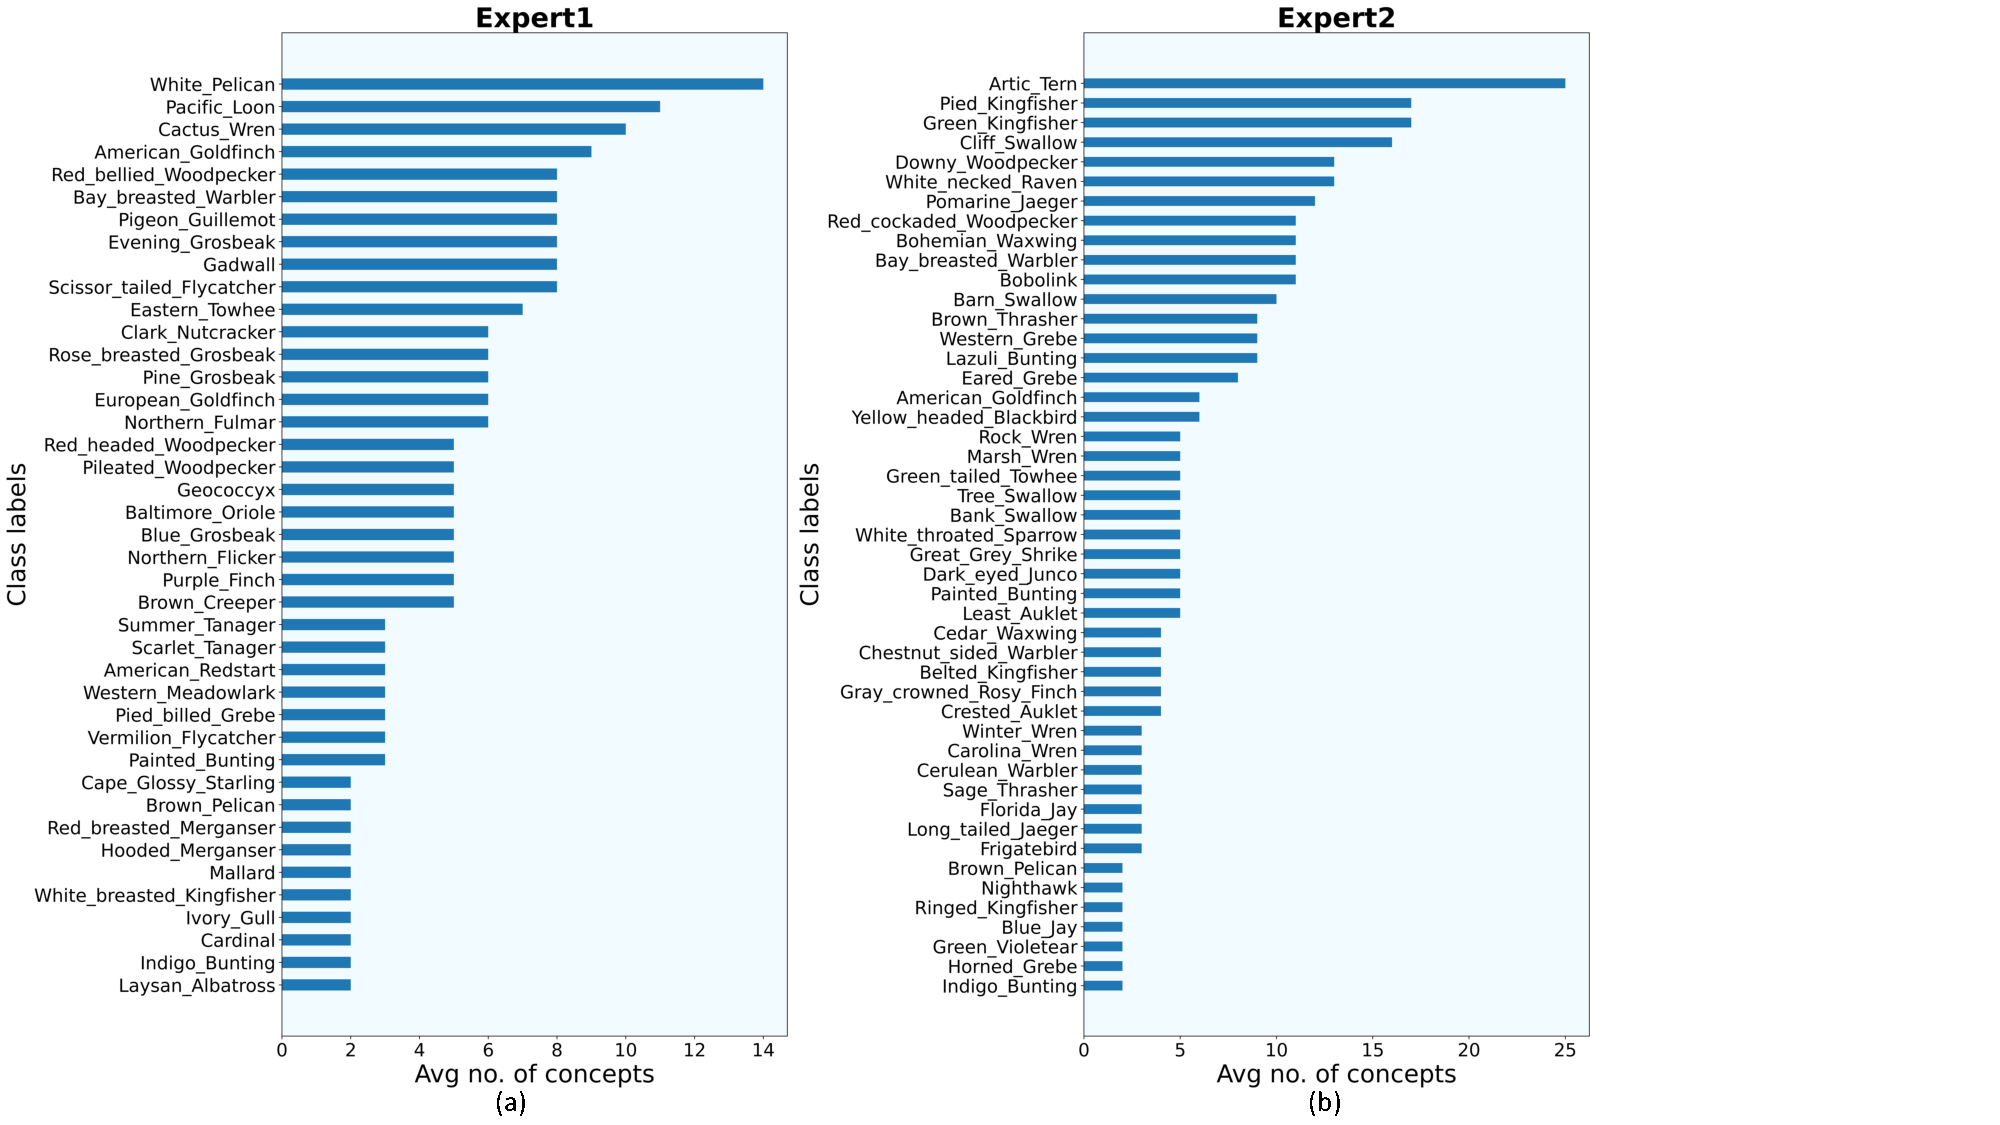
\includegraphics[width=14cm, height=13cm]
{figures/Supp/Avg_concept_class_VIT_cub_1.pdf}
\caption{Class labels (Bird species) vs. avg concepts using VIT as the backbone for CUB-200 by (a) Expert1 (b) Expert2. Each bar in this plot indicates the average number of concepts required to explain each sample of that bird species correctly. For example according to (a) expert1 requires 14 concepts to explain an instance of ``White Pelican''.}
\label{fig:vit_cub_concept_1_2}
\end{figure}

\begin{figure}
\centering
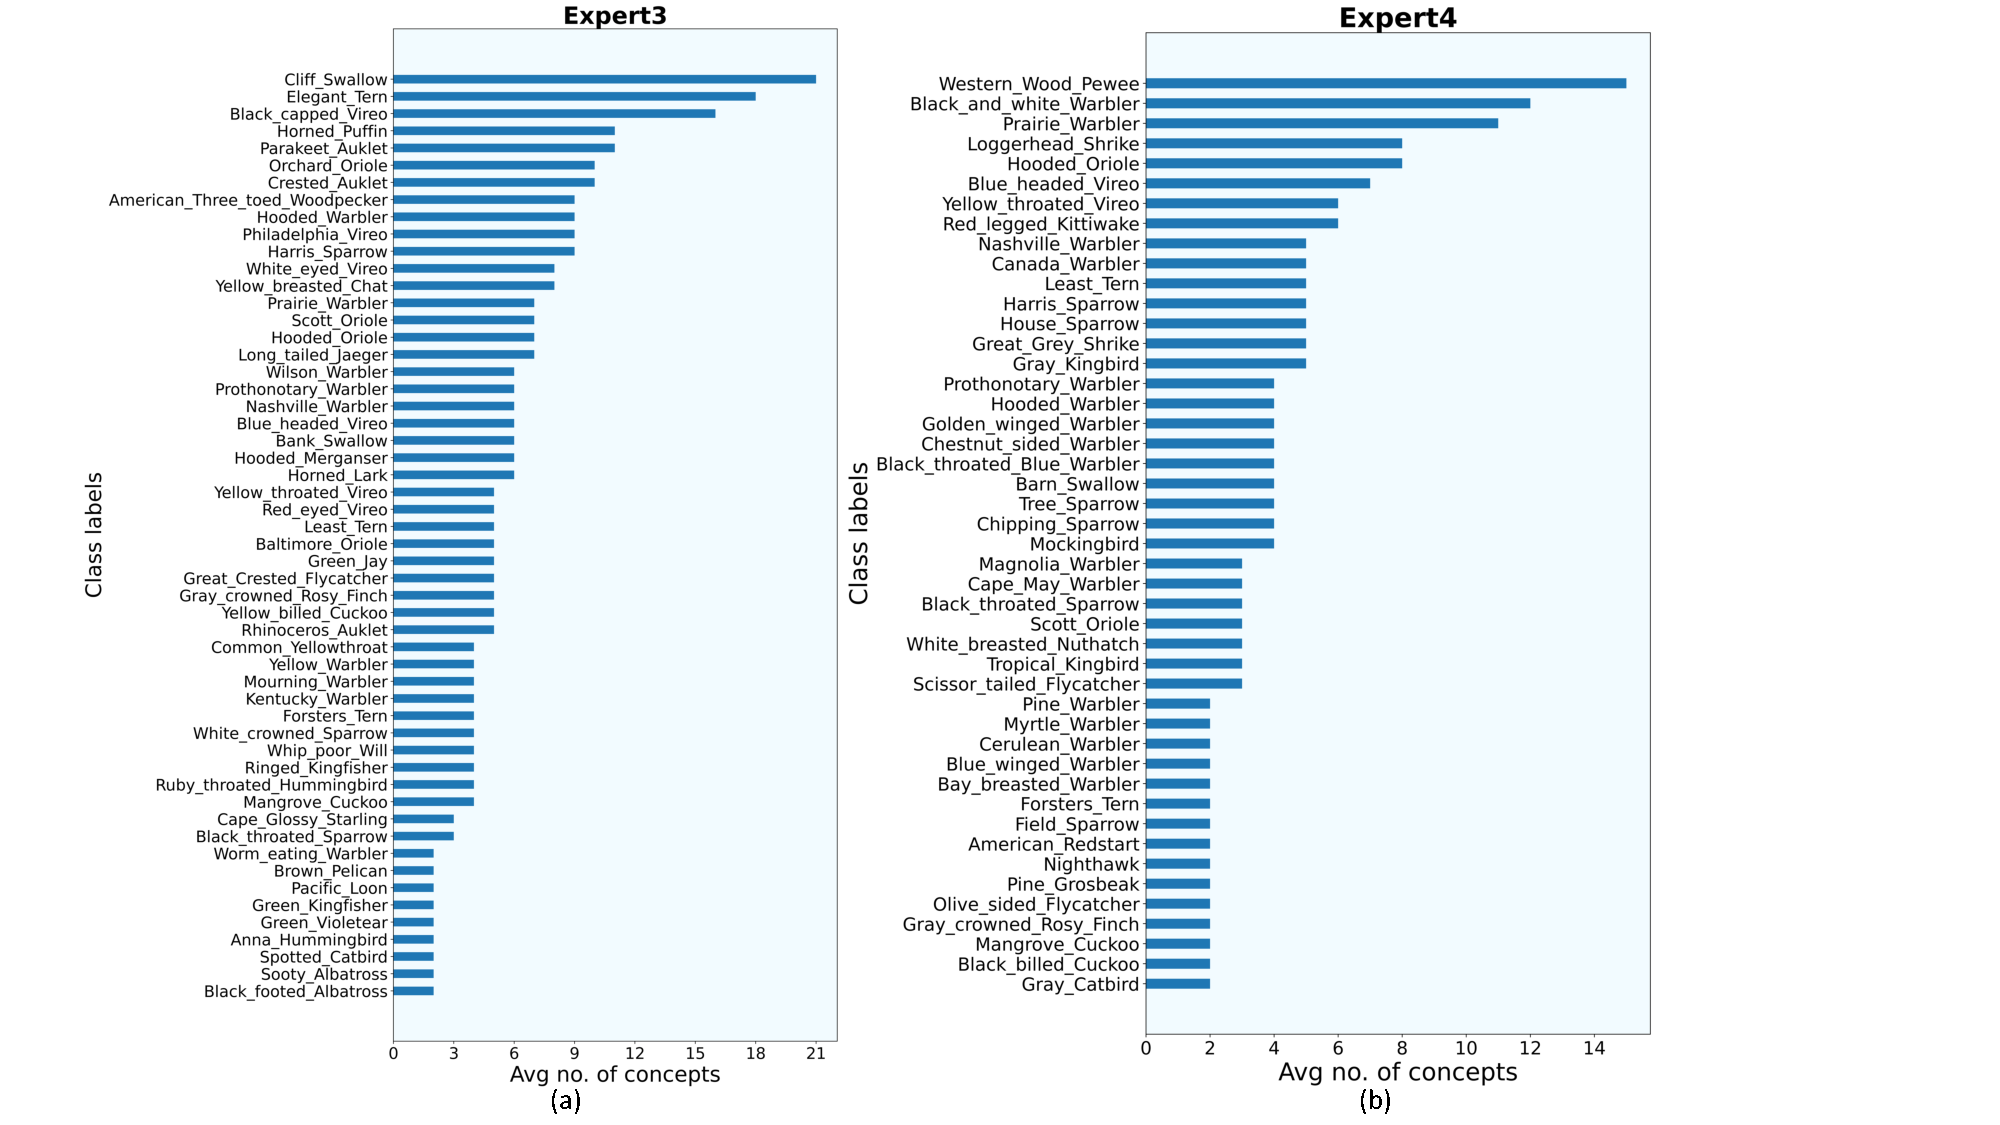
\includegraphics[width=14cm, height=13cm]
{figures/Supp/Avg_concept_class_VIT_cub_2.pdf}
\caption{Class labels (Bird species) vs. avg concepts using VIT as the backbone for CUB-200 by (a) Expert3 (b) Expert4. Each bar in this plot indicates the average number of concepts required to explain each sample of that bird species correctly. For example according to (a) expert3 requires 21 concepts to explain an instance of ``Cliff Swallow''.}
\label{fig:vit_cub_concept_3_4}
\end{figure}

\begin{figure}
\centering
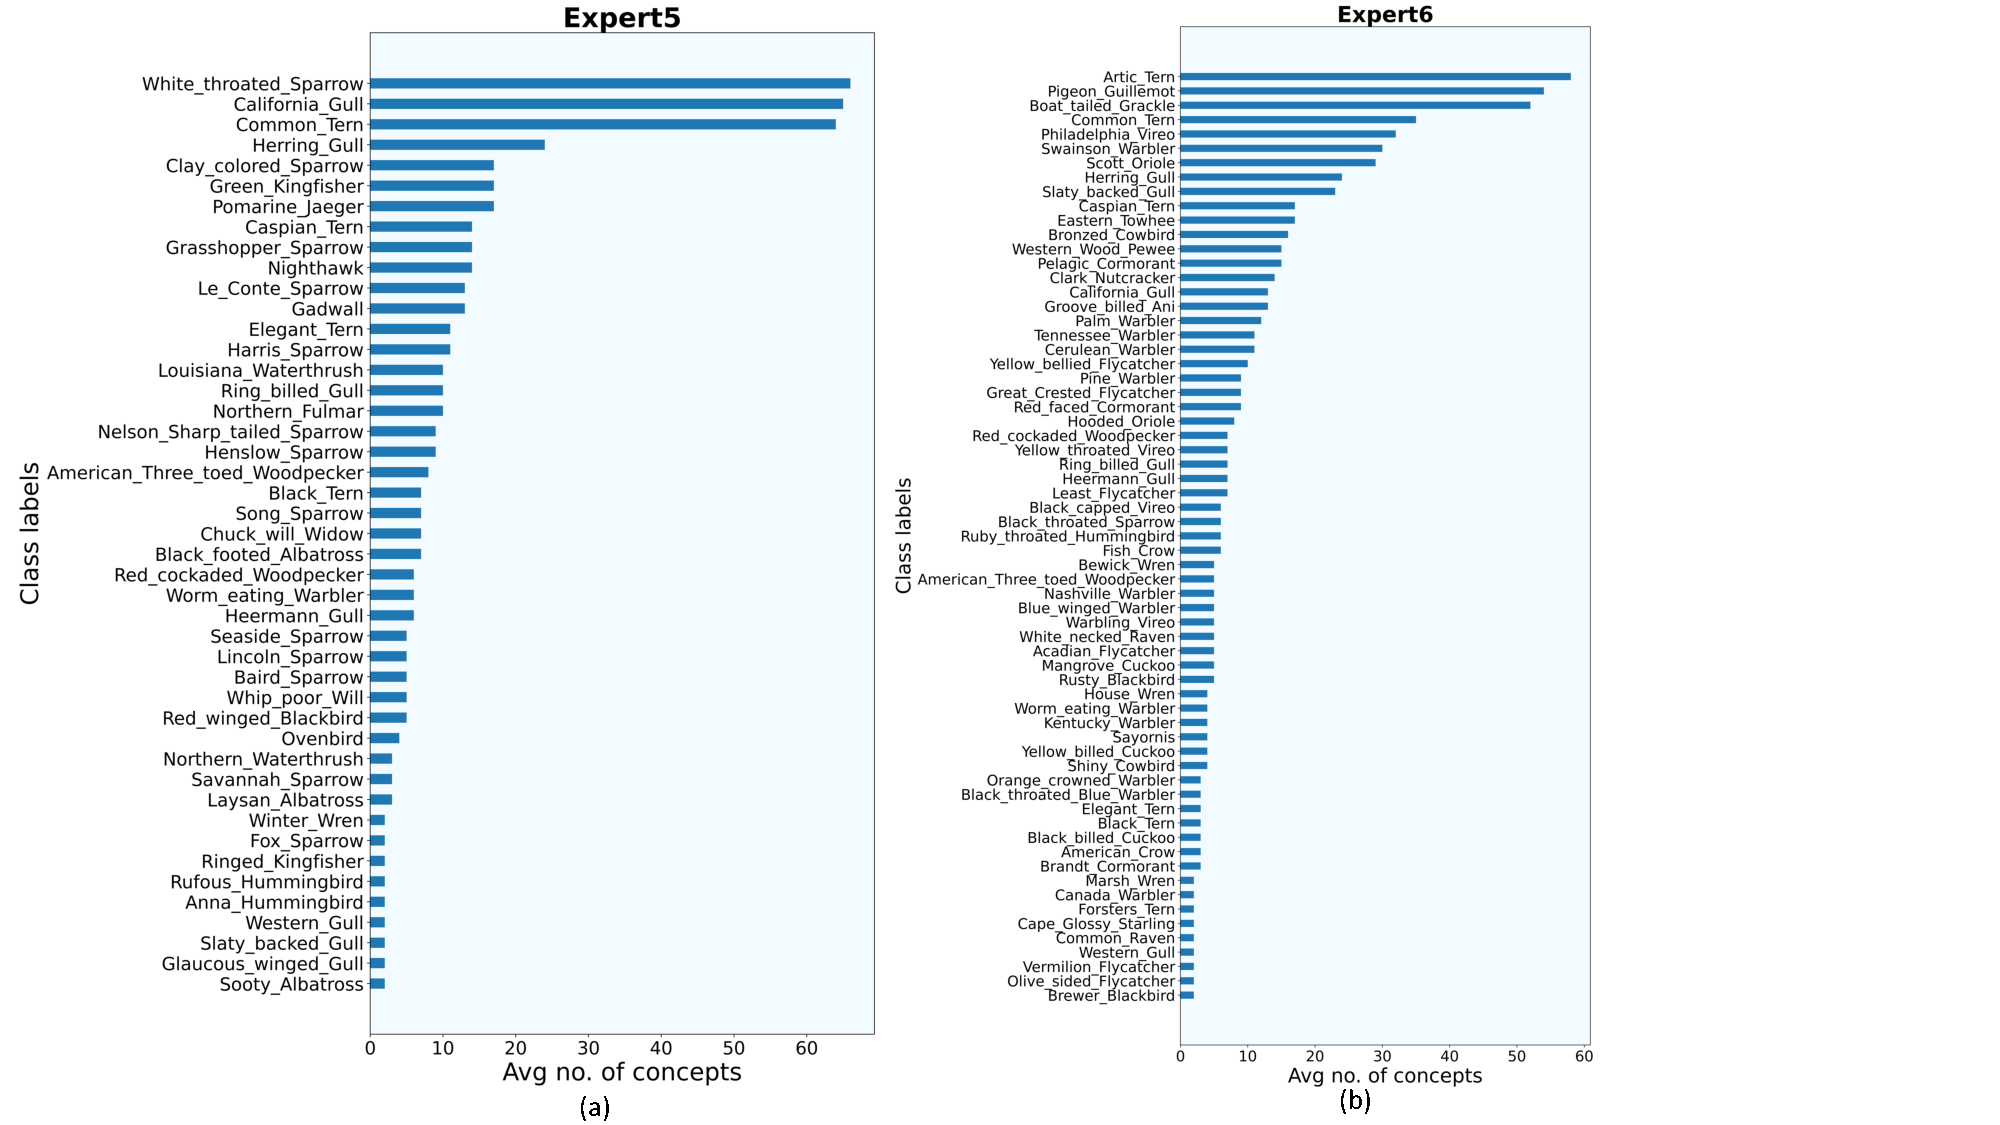
\includegraphics[width=14cm, height=13cm]
{figures/Supp/Avg_concept_class_VIT_cub_3.pdf}
\caption{Class labels (Bird species) vs. avg concepts using VIT as the backbone for CUB-200 by (a) Expert5 (b) Expert6. Each bar in this plot indicates the average number of concepts required to explain each sample of that bird species correctly. For example according to (a) expert5 requires approximately 65 concepts to explain an instance of ``White throated sparrow''.}
\label{fig:vit_cub_concept_5_6}
\end{figure}

% CNN
\begin{figure}
\centering
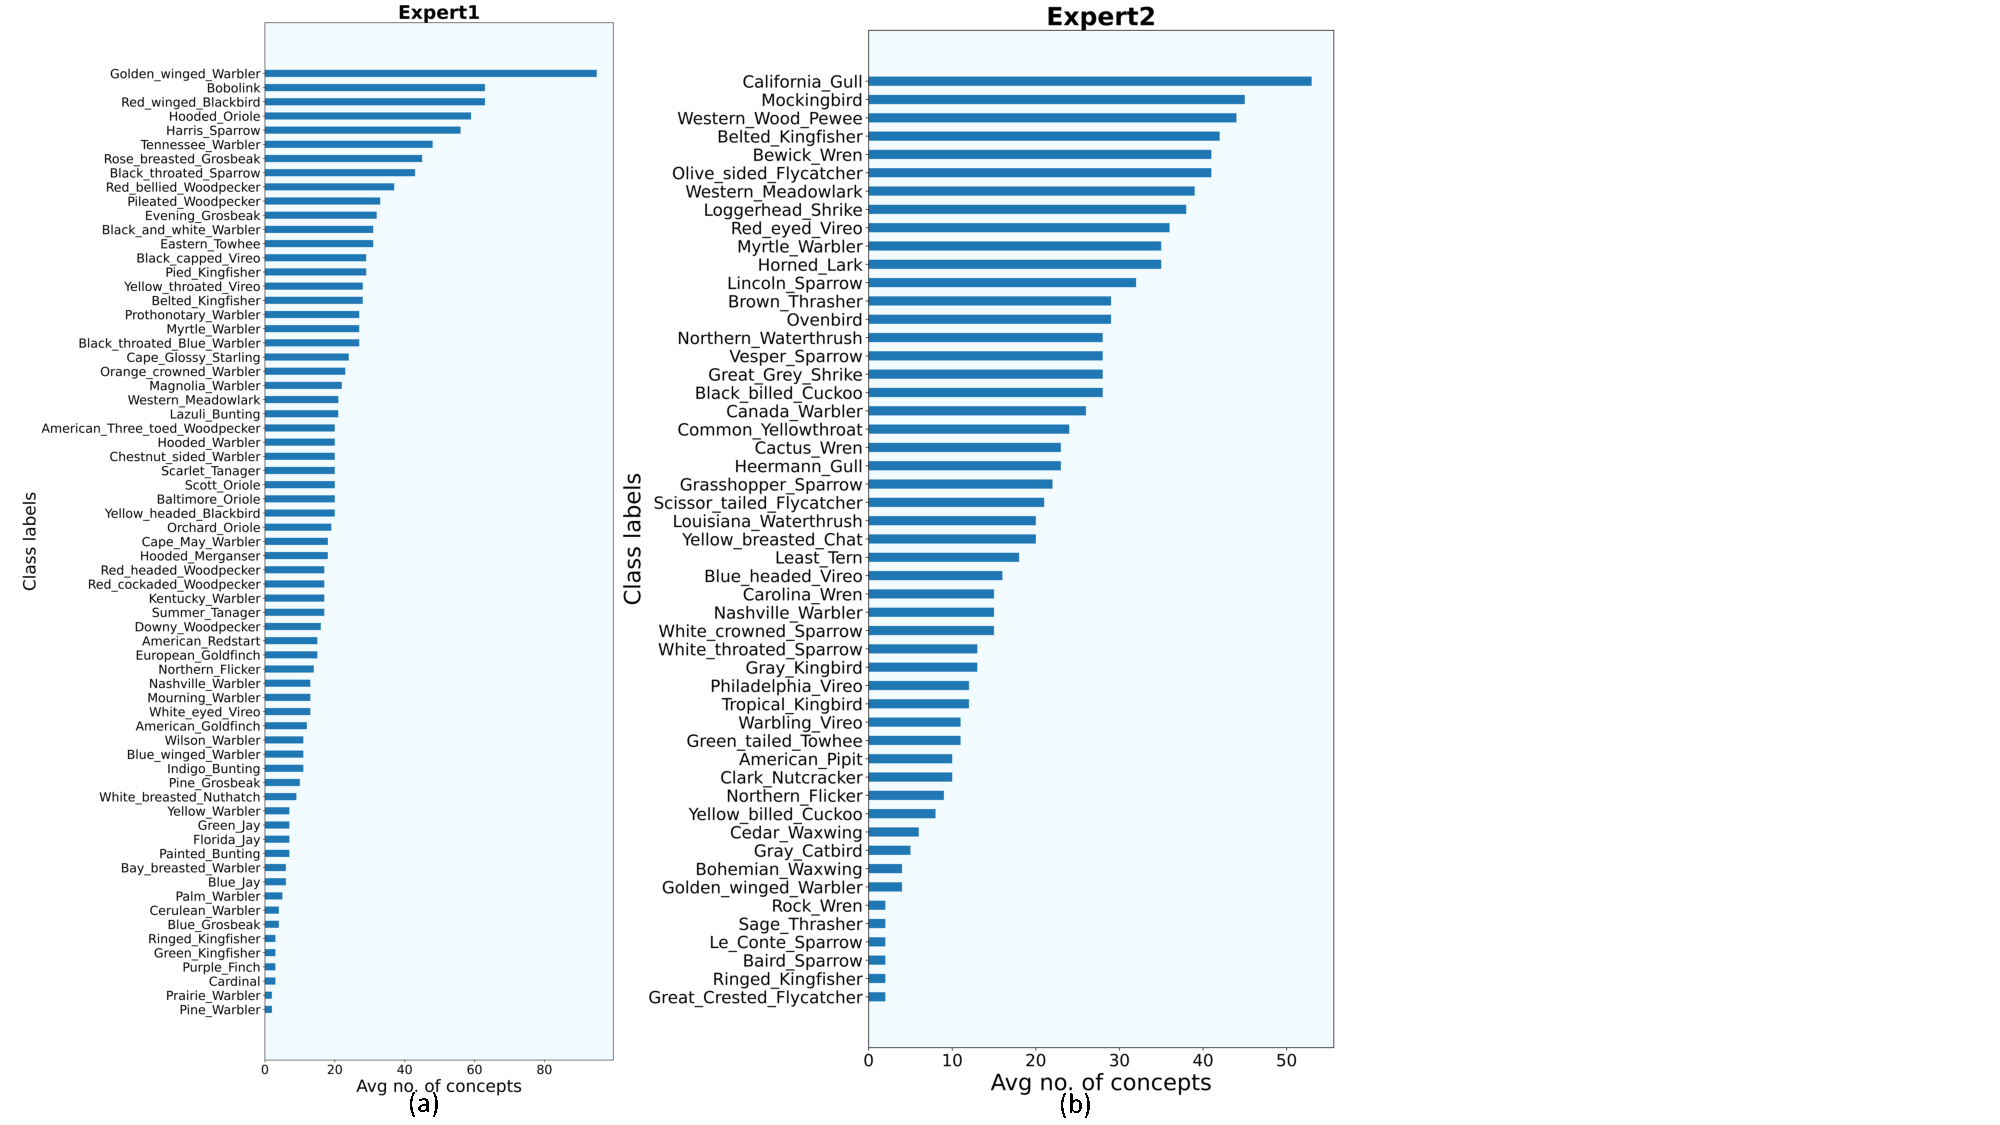
\includegraphics[width=15cm, height=13cm]
{figures/Supp/Avg_concept_class_CNN_cub_1.pdf}
\caption{Class labels (Bird species) vs. avg concepts using ResNet-101 as the backbone for CUB-200 by (a) Expert1 (b) Expert2. Each bar in this plot indicates the average number of concepts required to explain each sample of that bird species correctly. For example according to (a) expert1 requires approximately 85 concepts to explain an instance of ``Golden winged warbler''.}
\label{fig:cnn_cub_concept_1_2}
\end{figure}

\begin{figure}
\centering
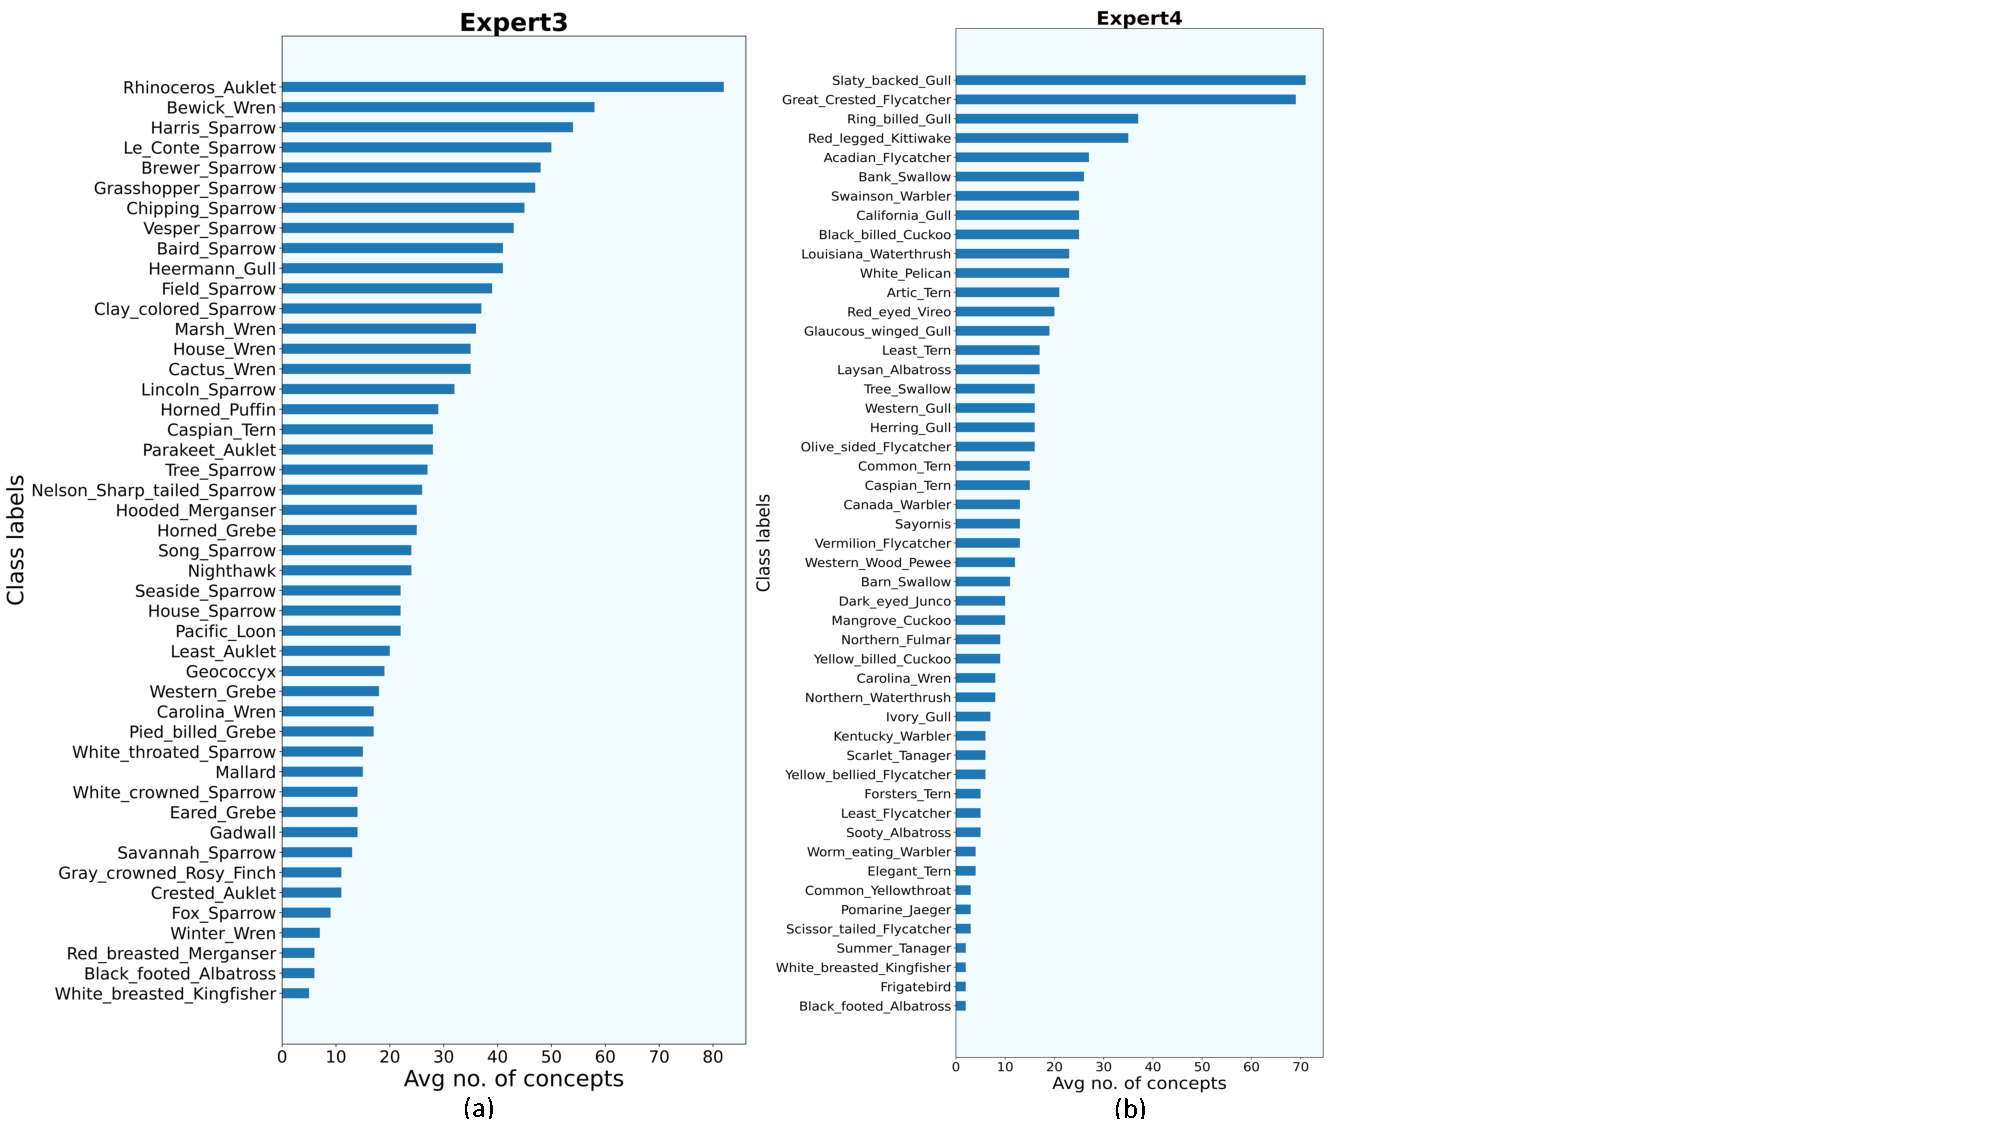
\includegraphics[width=15cm, height=13cm]
{figures/Supp/Avg_concept_class_CNN_cub_2.pdf}
\caption{Class labels (Bird species) vs. avg concepts using  ResNet-101 as the backbone for CUB-200 by (a) Expert3 (b) Expert4. Each bar in this plot indicates the average number of concepts required to explain each sample of that bird species correctly. For example according to (a) expert3 requires approximately 82 concepts to explain an instance of ``Rhinoceros auklet''.}
\label{fig:cnn_cub_concept_3_4}
\end{figure}

\begin{figure}
\centering
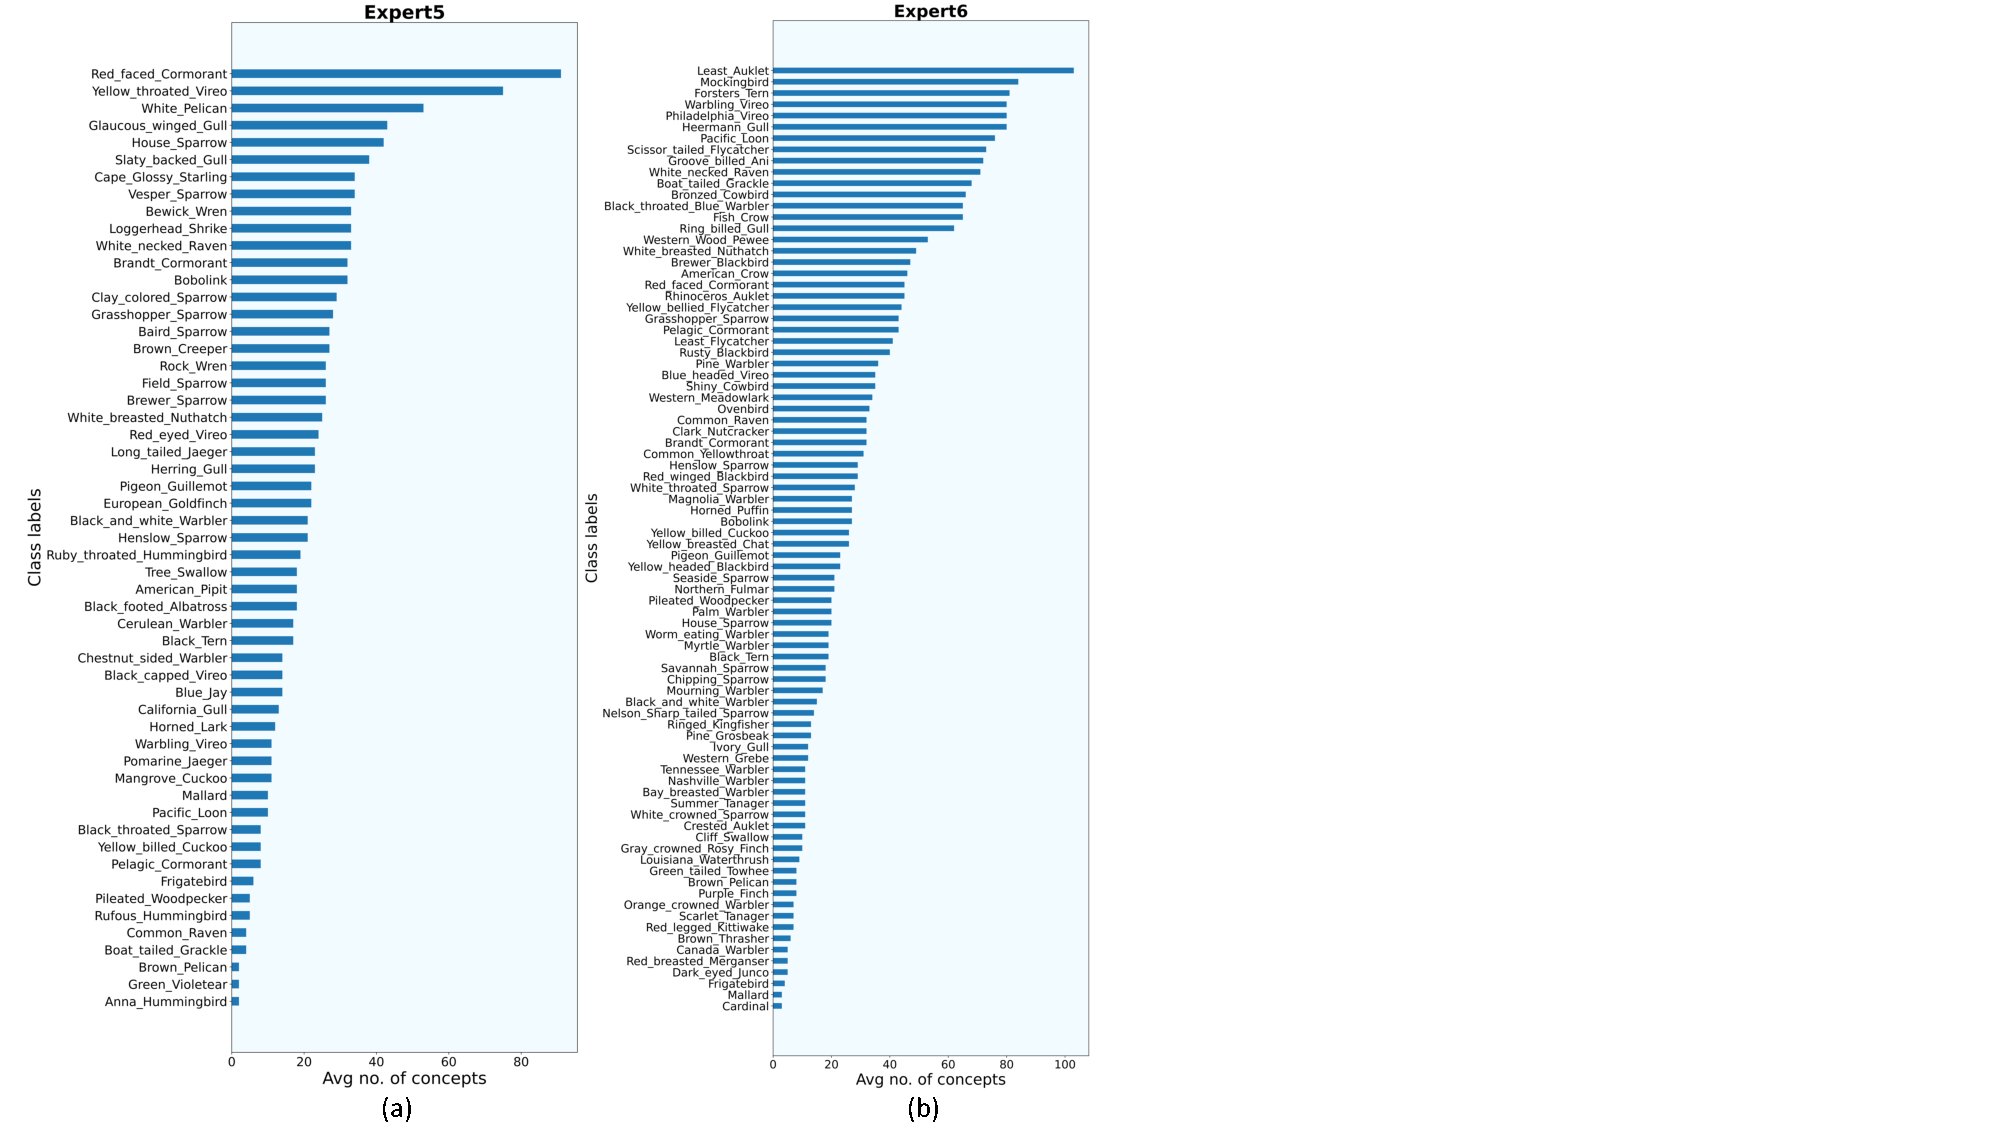
\includegraphics[width=1\linewidth]
{figures/Supp/Avg_concept_class_CNN_cub_3.pdf}
\caption{Class labels (Bird species) vs. avg concepts using  ResNet-101 as the backbone for CUB-200 by (a) Expert5 (b) Expert6. Each bar in this plot indicates the average number of concepts required to explain each sample of that bird species correctly. For example according to (a) expert5 requires approximately 85 concepts to explain an instance of ``Red faced carmorant''.}
\label{fig:cnn_cub_concept_5_6}
\end{figure}

\begin{figure}
\centering
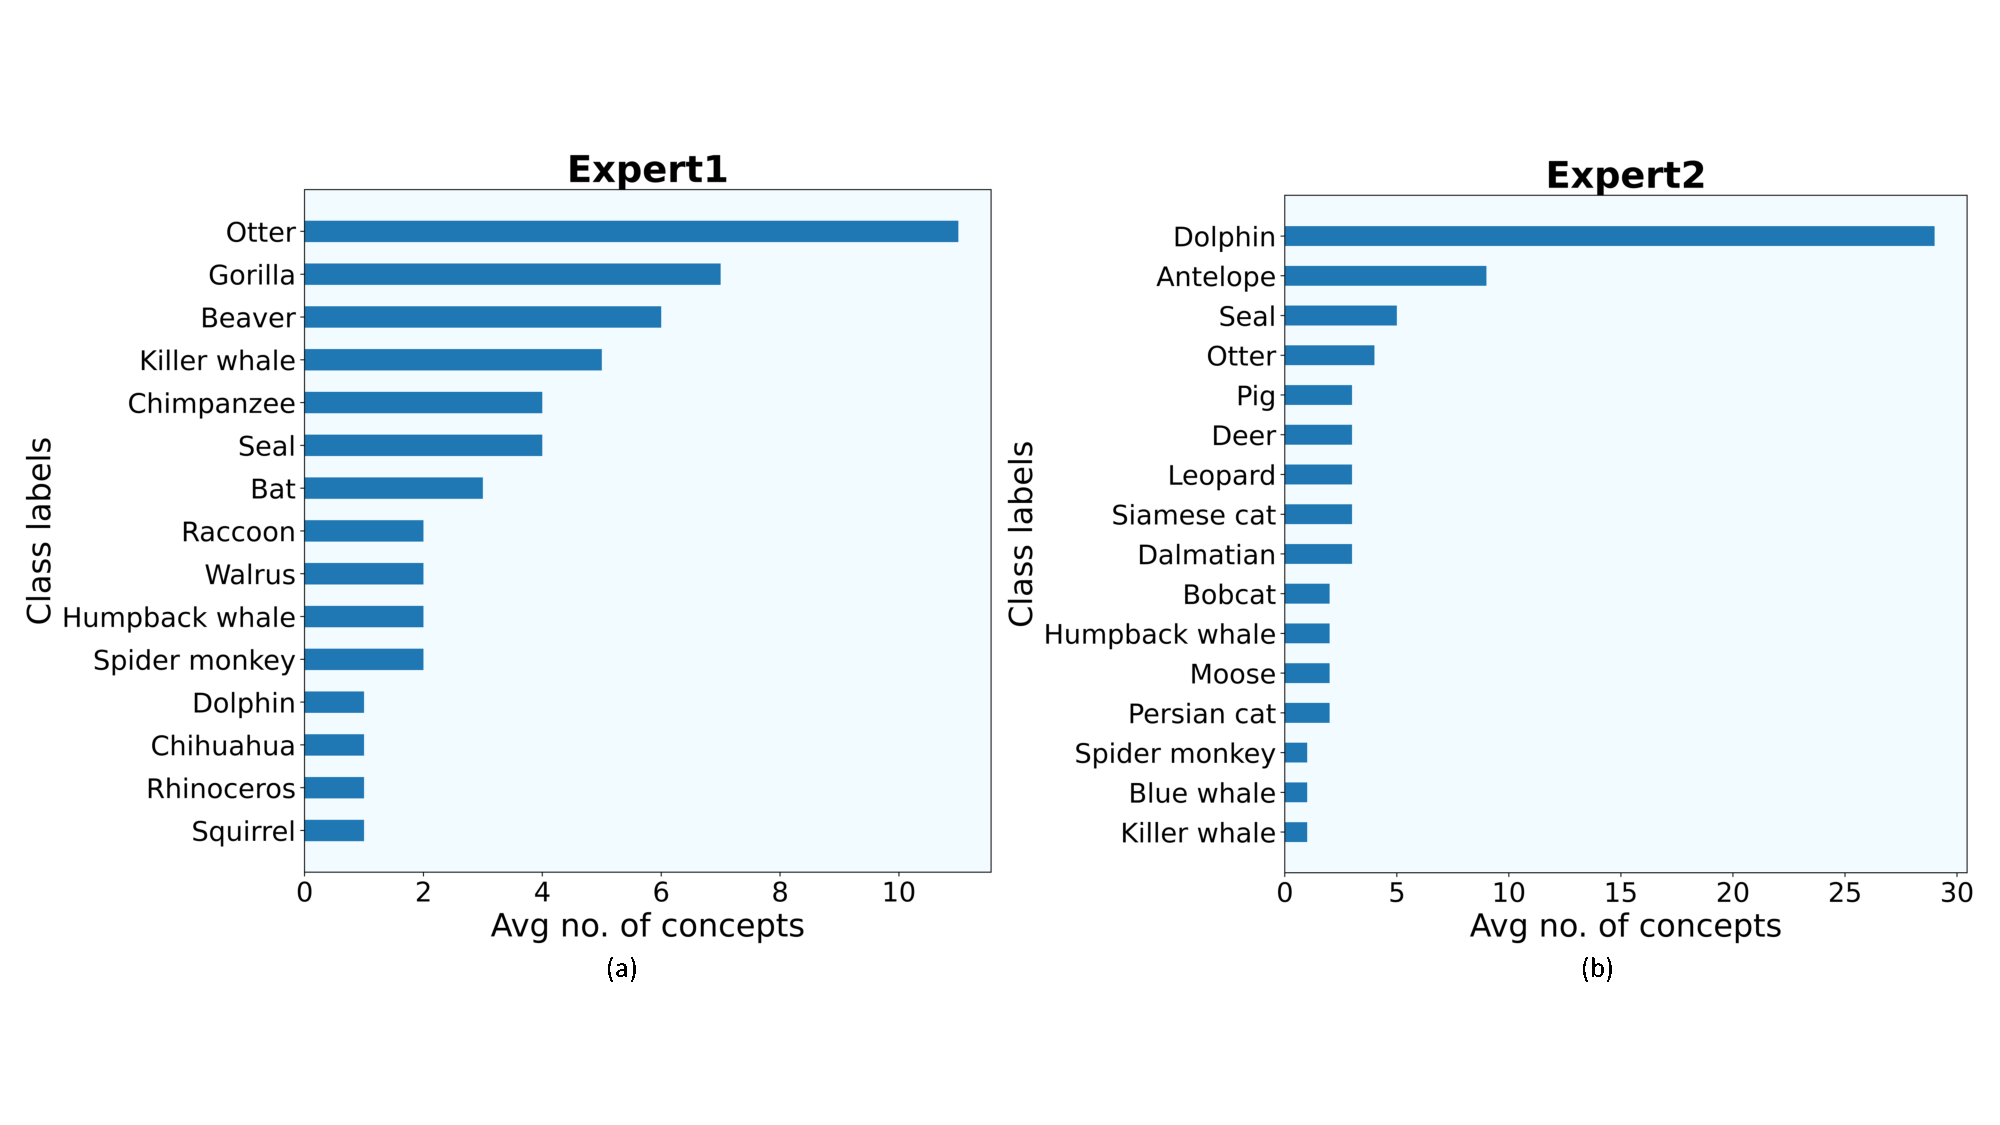
\includegraphics[width=1\linewidth]
{figures/Supp/Avg_concept_class_VIT_Awa2_1.pdf}
\caption{Class labels (Animal species) vs. avg concepts using VIT as the backbone for Awa2. Each bar in this plot indicates the average number of concepts required to explain each sample of that animal species correctly. For example according to (c) expert1 requires approximately 12 concepts to explain an instance of ``Otter''.}
\label{fig:Awa2_VIT_a}
\end{figure}

\begin{figure}
\centering
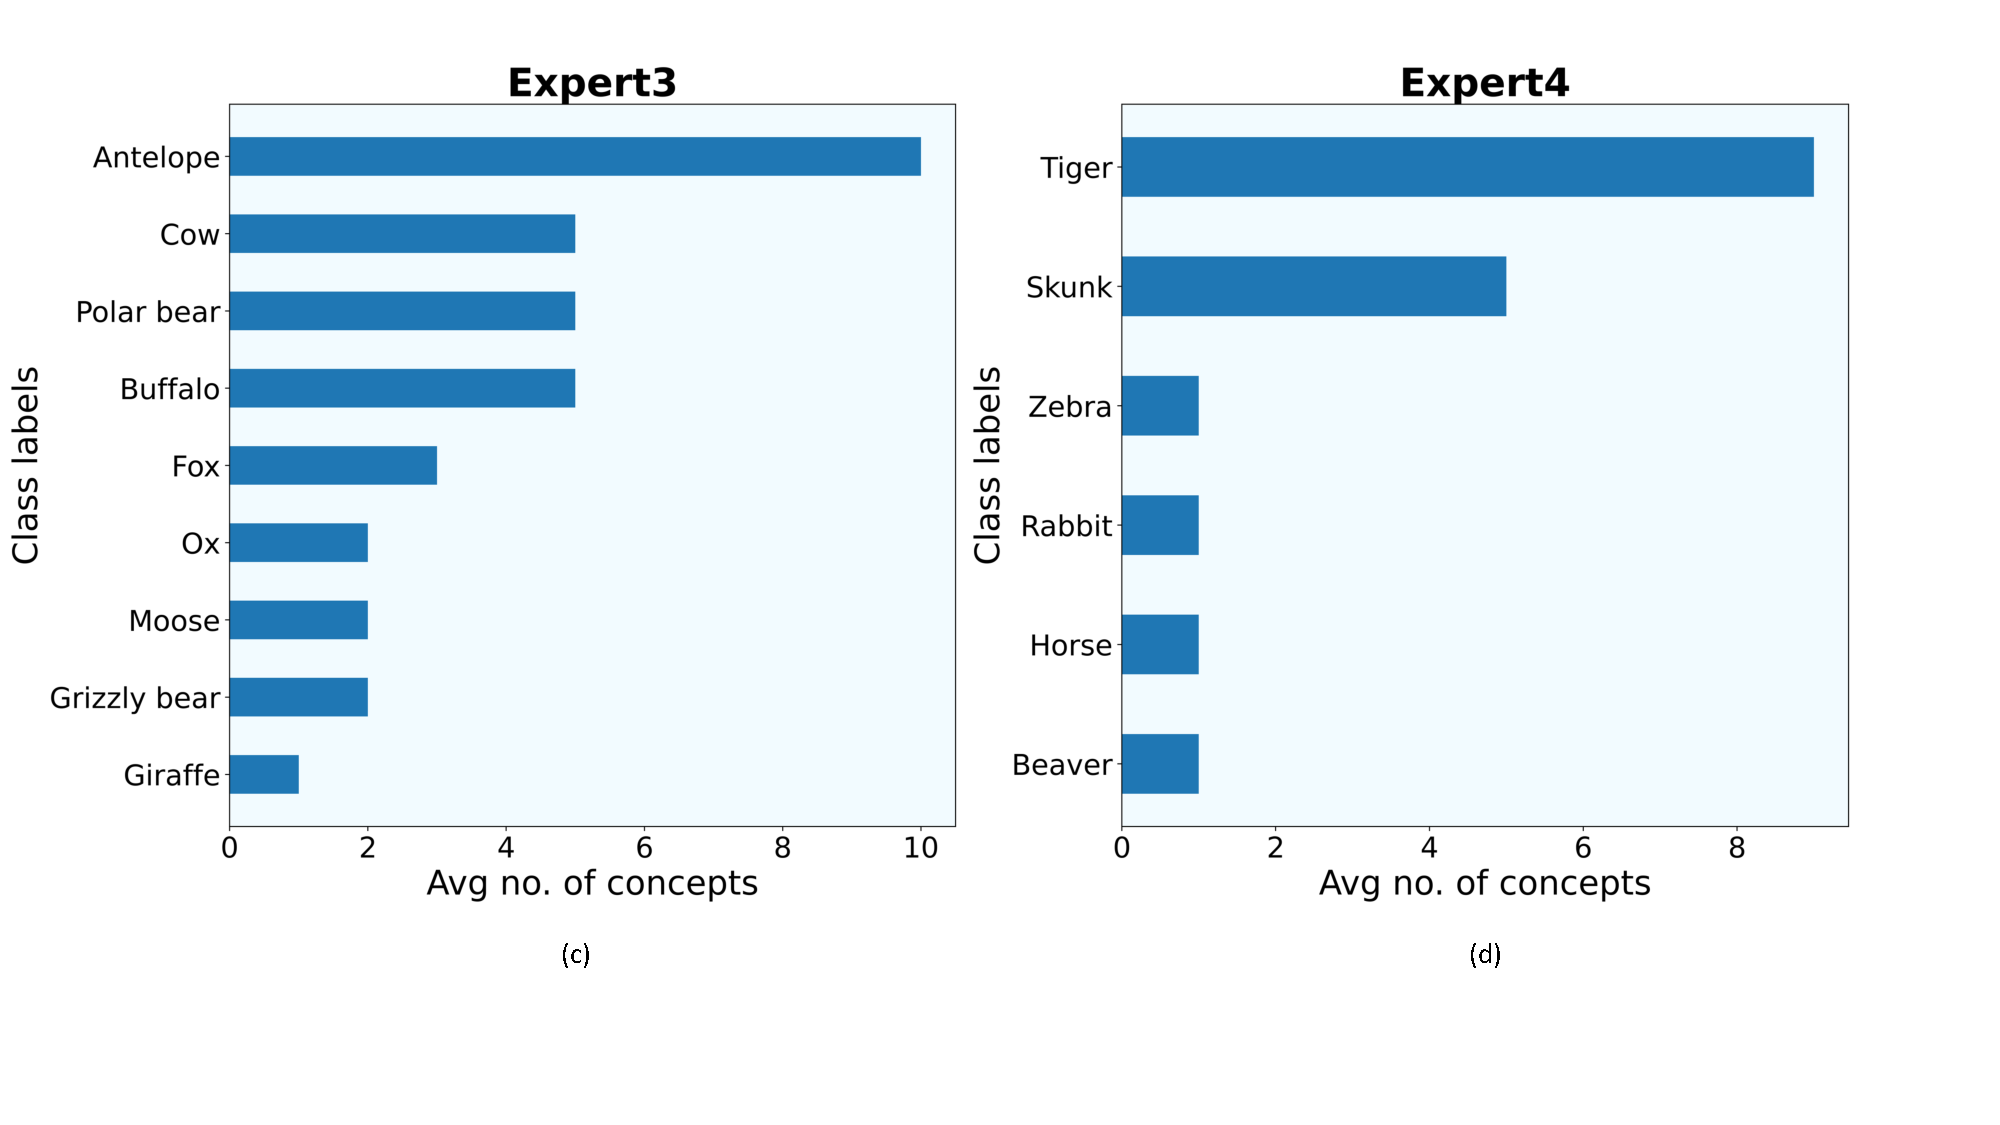
\includegraphics[width=1\linewidth]
{figures/Supp/Avg_concept_class_VIT_Awa2_2.pdf}
\caption{Class labels (Animal species) vs. avg concepts using VIT as the backbone for Awa2. Each bar in this plot indicates the average number of concepts required to explain each sample of that animal species correctly. For example according to (c) expert3 requires approximately 10 concepts to explain an instance of ``Antelope''.}
\label{fig:Awa2_VIT_b}
\end{figure}

\begin{figure}
\centering
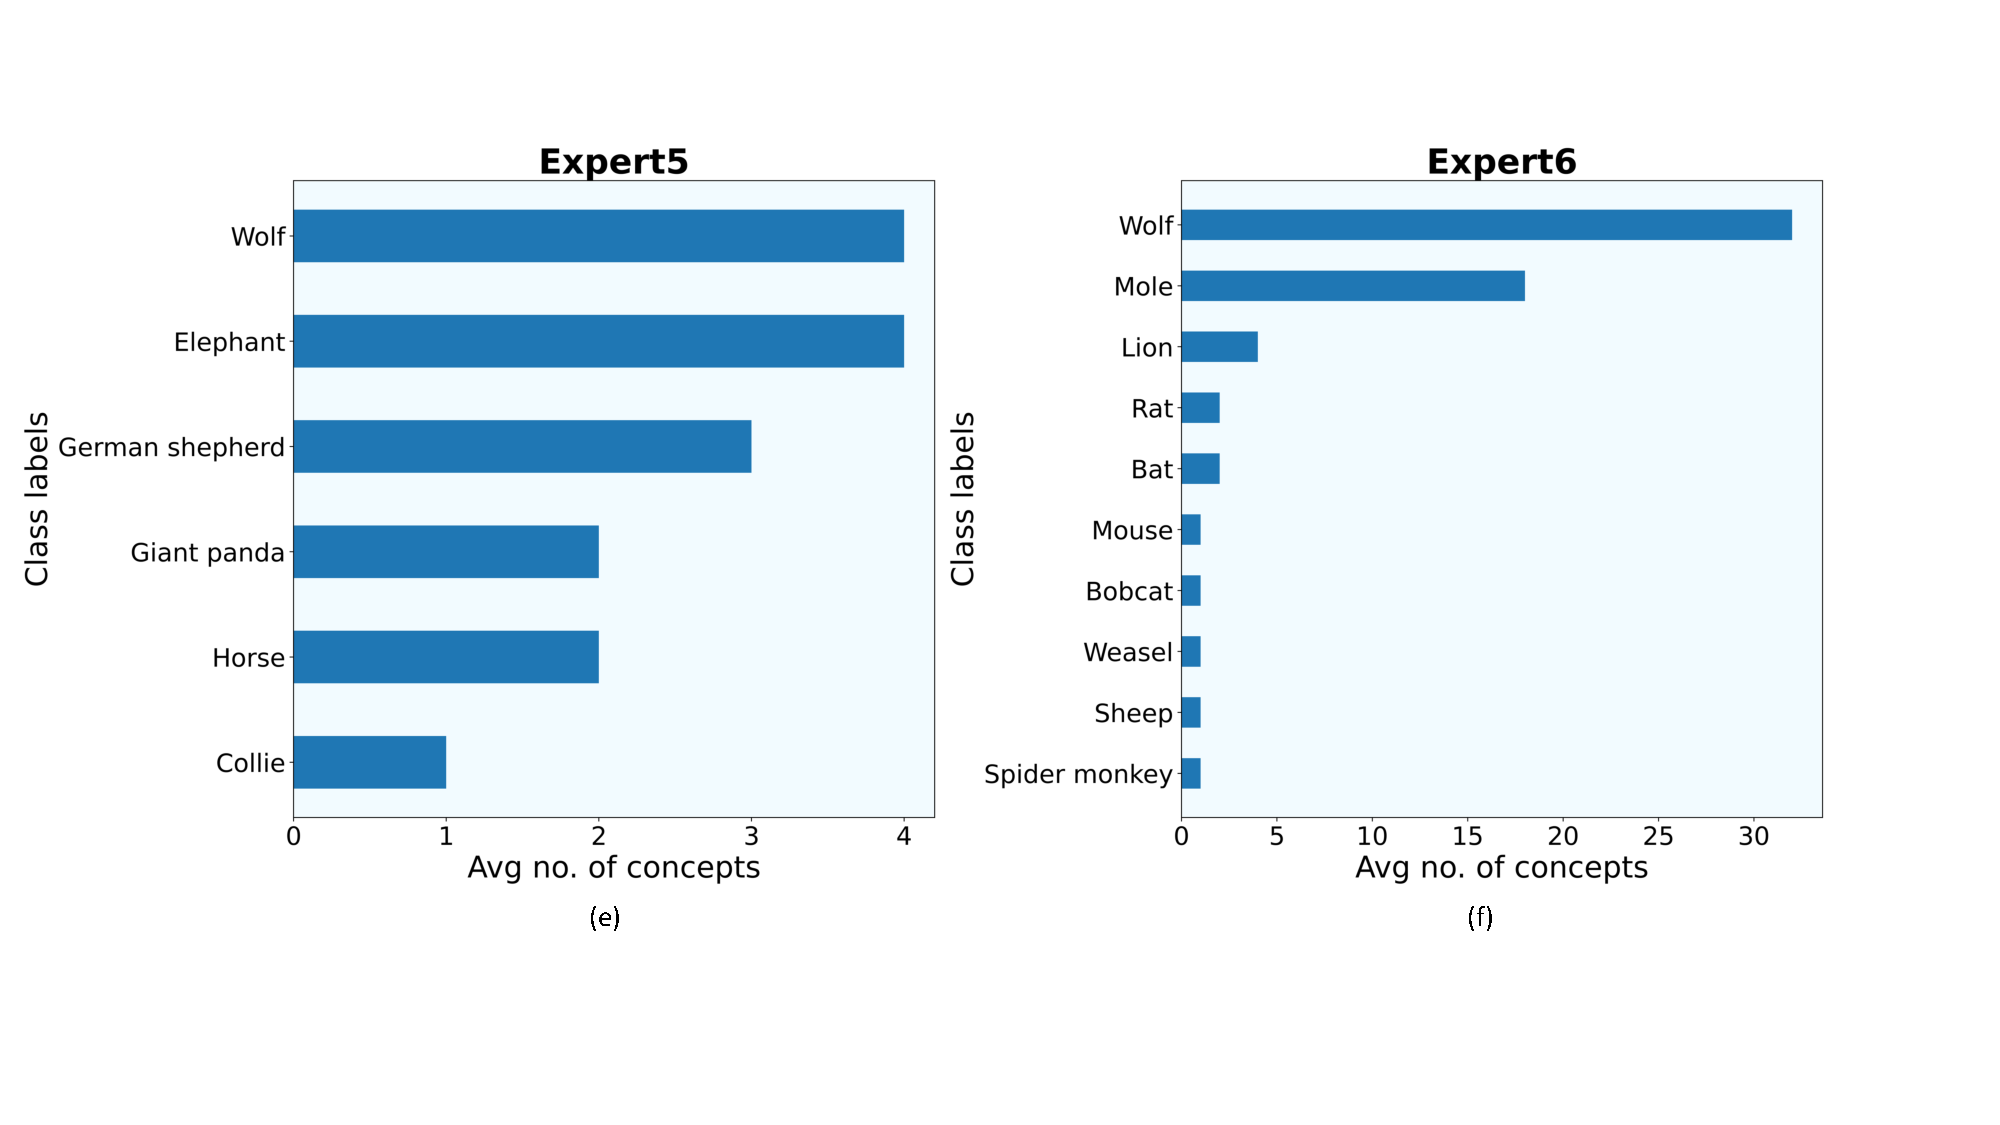
\includegraphics[width=1\linewidth]
{figures/Supp/Avg_concept_class_VIT_Awa2_3.pdf}
\caption{Class labels (Animal species) vs. avg concepts using VIT as the backbone for Awa2. Each bar in this plot indicates the average number of concepts required to explain each sample of that animal species correctly. For example according to (e) expert5 requires approximately 4 concepts to explain an instance of ``Antelope''.}
\label{fig:Awa2_VIT_c}
\end{figure}

\begin{figure}[t]
\centering
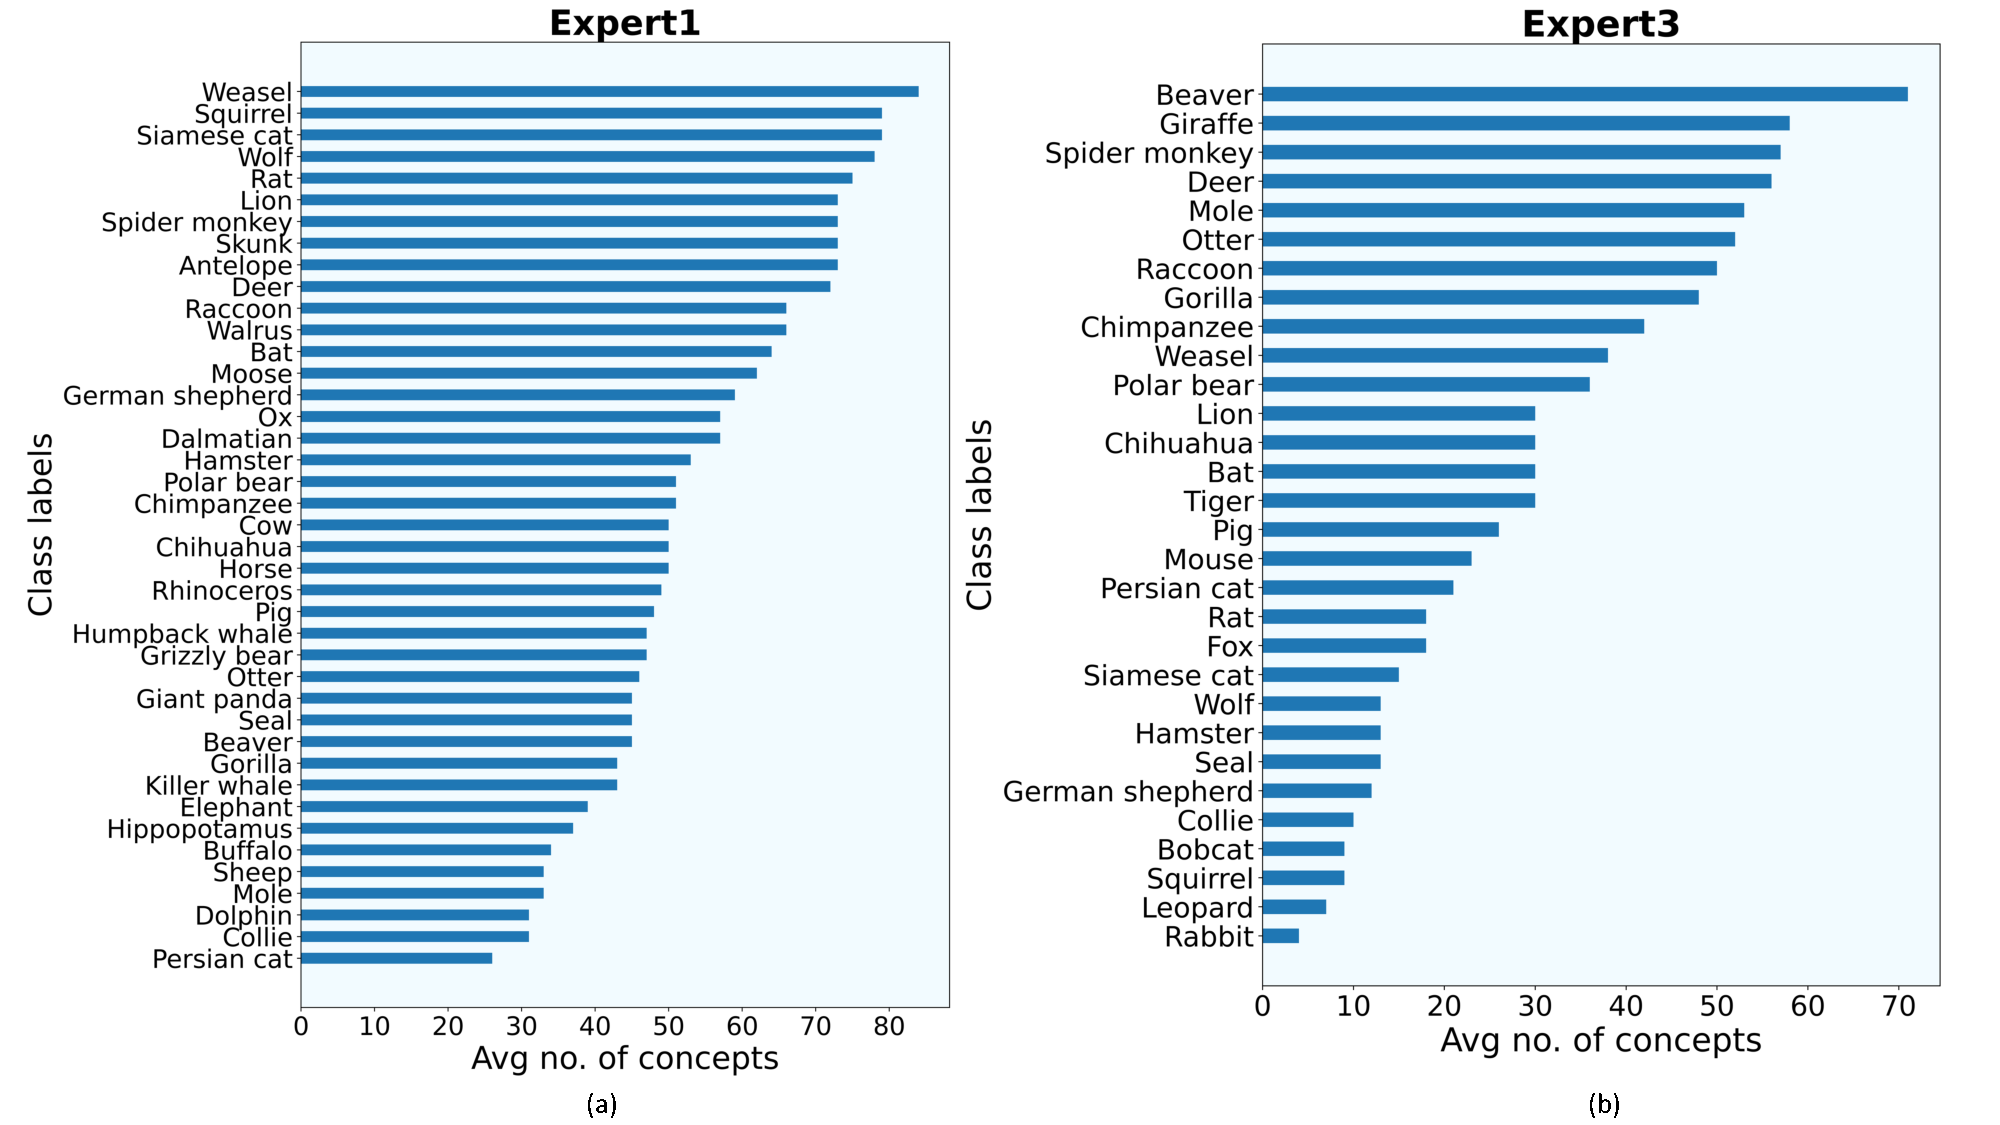
\includegraphics[width=1\linewidth]
{figures/Supp/Avg_concept_class_CNN_Awa2_1.pdf}
\caption{Class labels (Animal species) vs. avg concepts using ResNet-101 as the backbone for Awa2. Each bar in this plot indicates the average number of concepts required to explain each sample of that animal species correctly. For example according to (a) expert1 requires approximately 80 concepts to explain an instance of ``Weasel''.}
\label{fig:Awa2_CNN_a}
\end{figure}

\begin{figure}
\centering
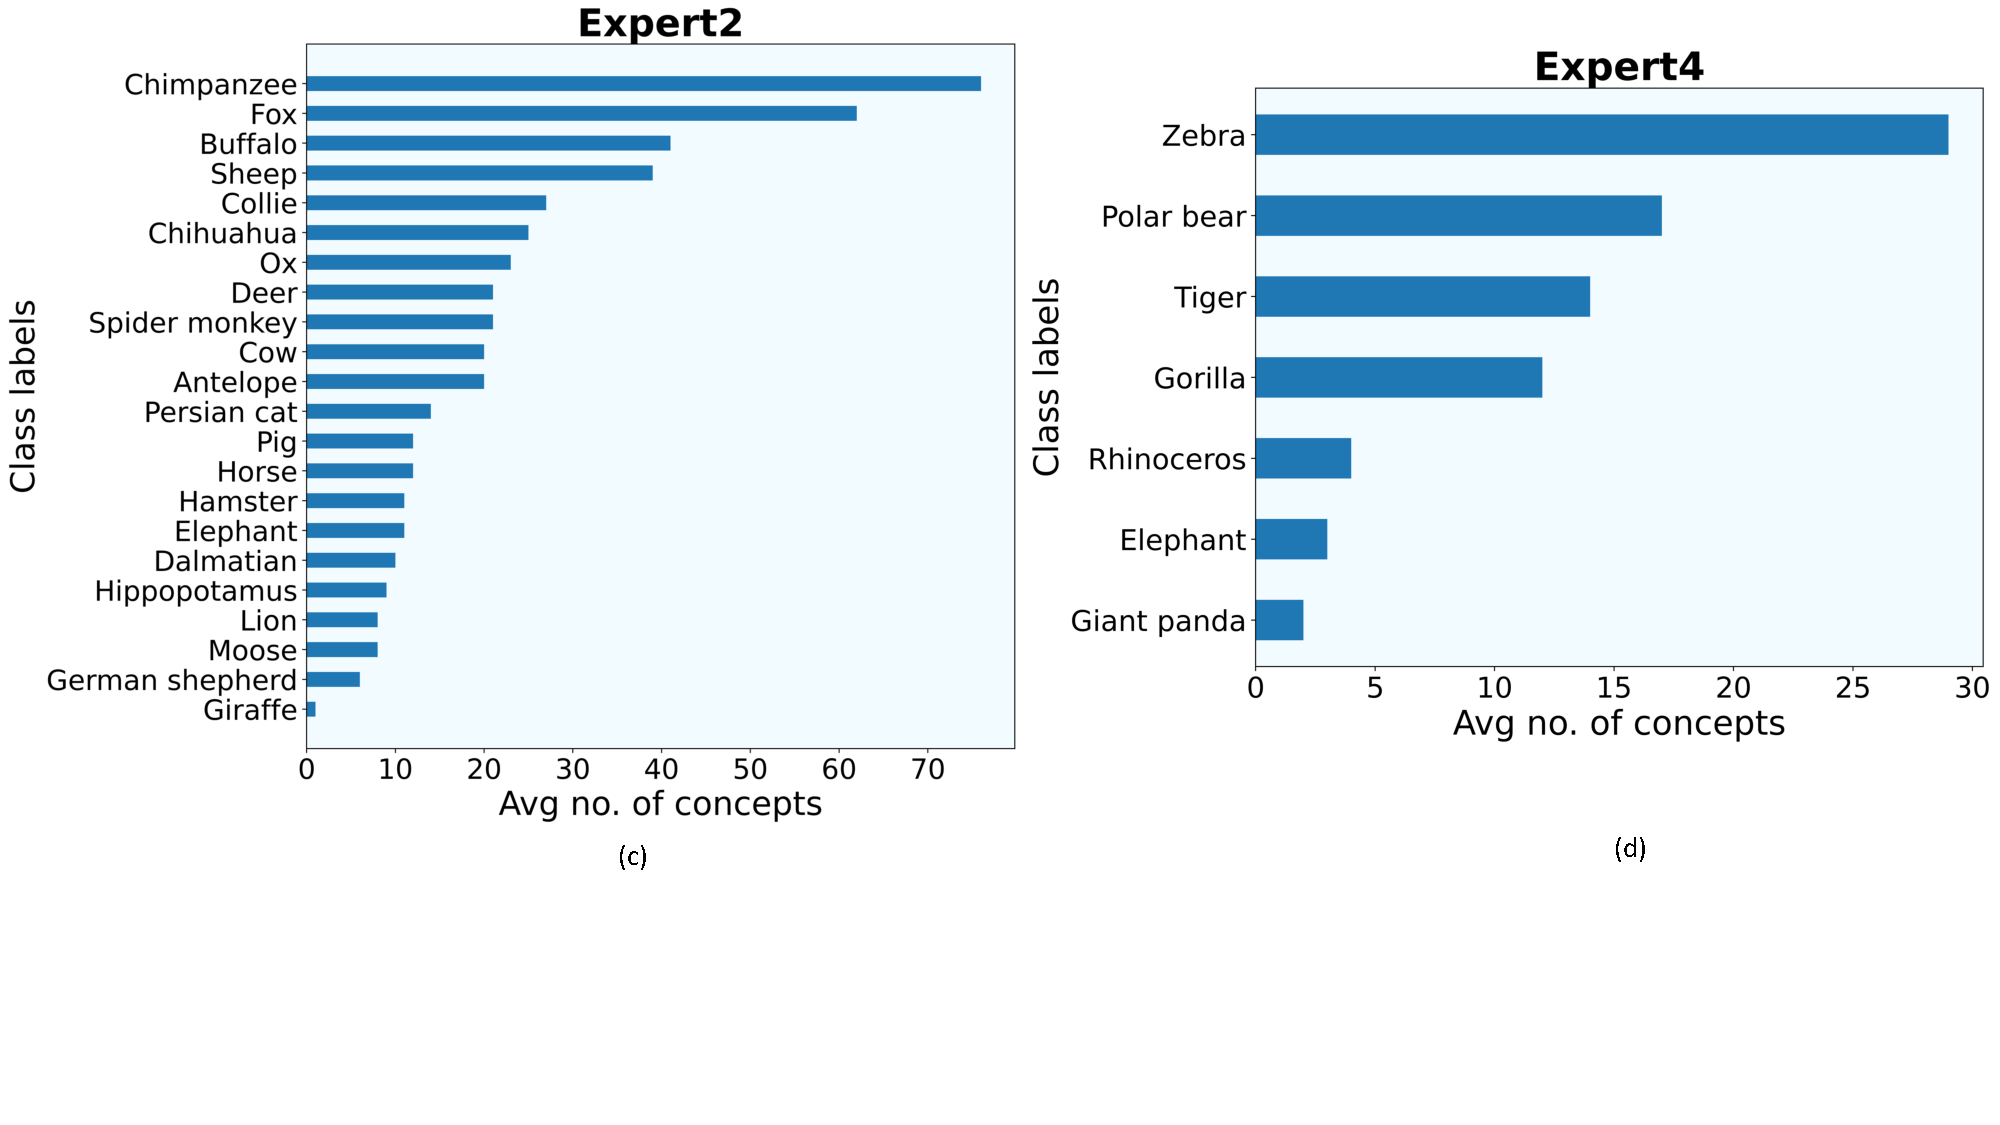
\includegraphics[width=1\linewidth]
{figures/Supp/Avg_concept_class_CNN_Awa2_2.pdf}
\caption{Class labels (Animal species) vs. avg concepts using ResNet-101 as the backbone for Awa2. Each bar in this plot indicates the average number of concepts required to explain each sample of that animal species correctly. For example according to (b) expert2 requires approximately 72 concepts to explain an instance of ``Chimpanzee''.}
\label{fig:Awa2_CNN_b}
\end{figure}



% \begin{figure}
%   \centering
%   \subfloat{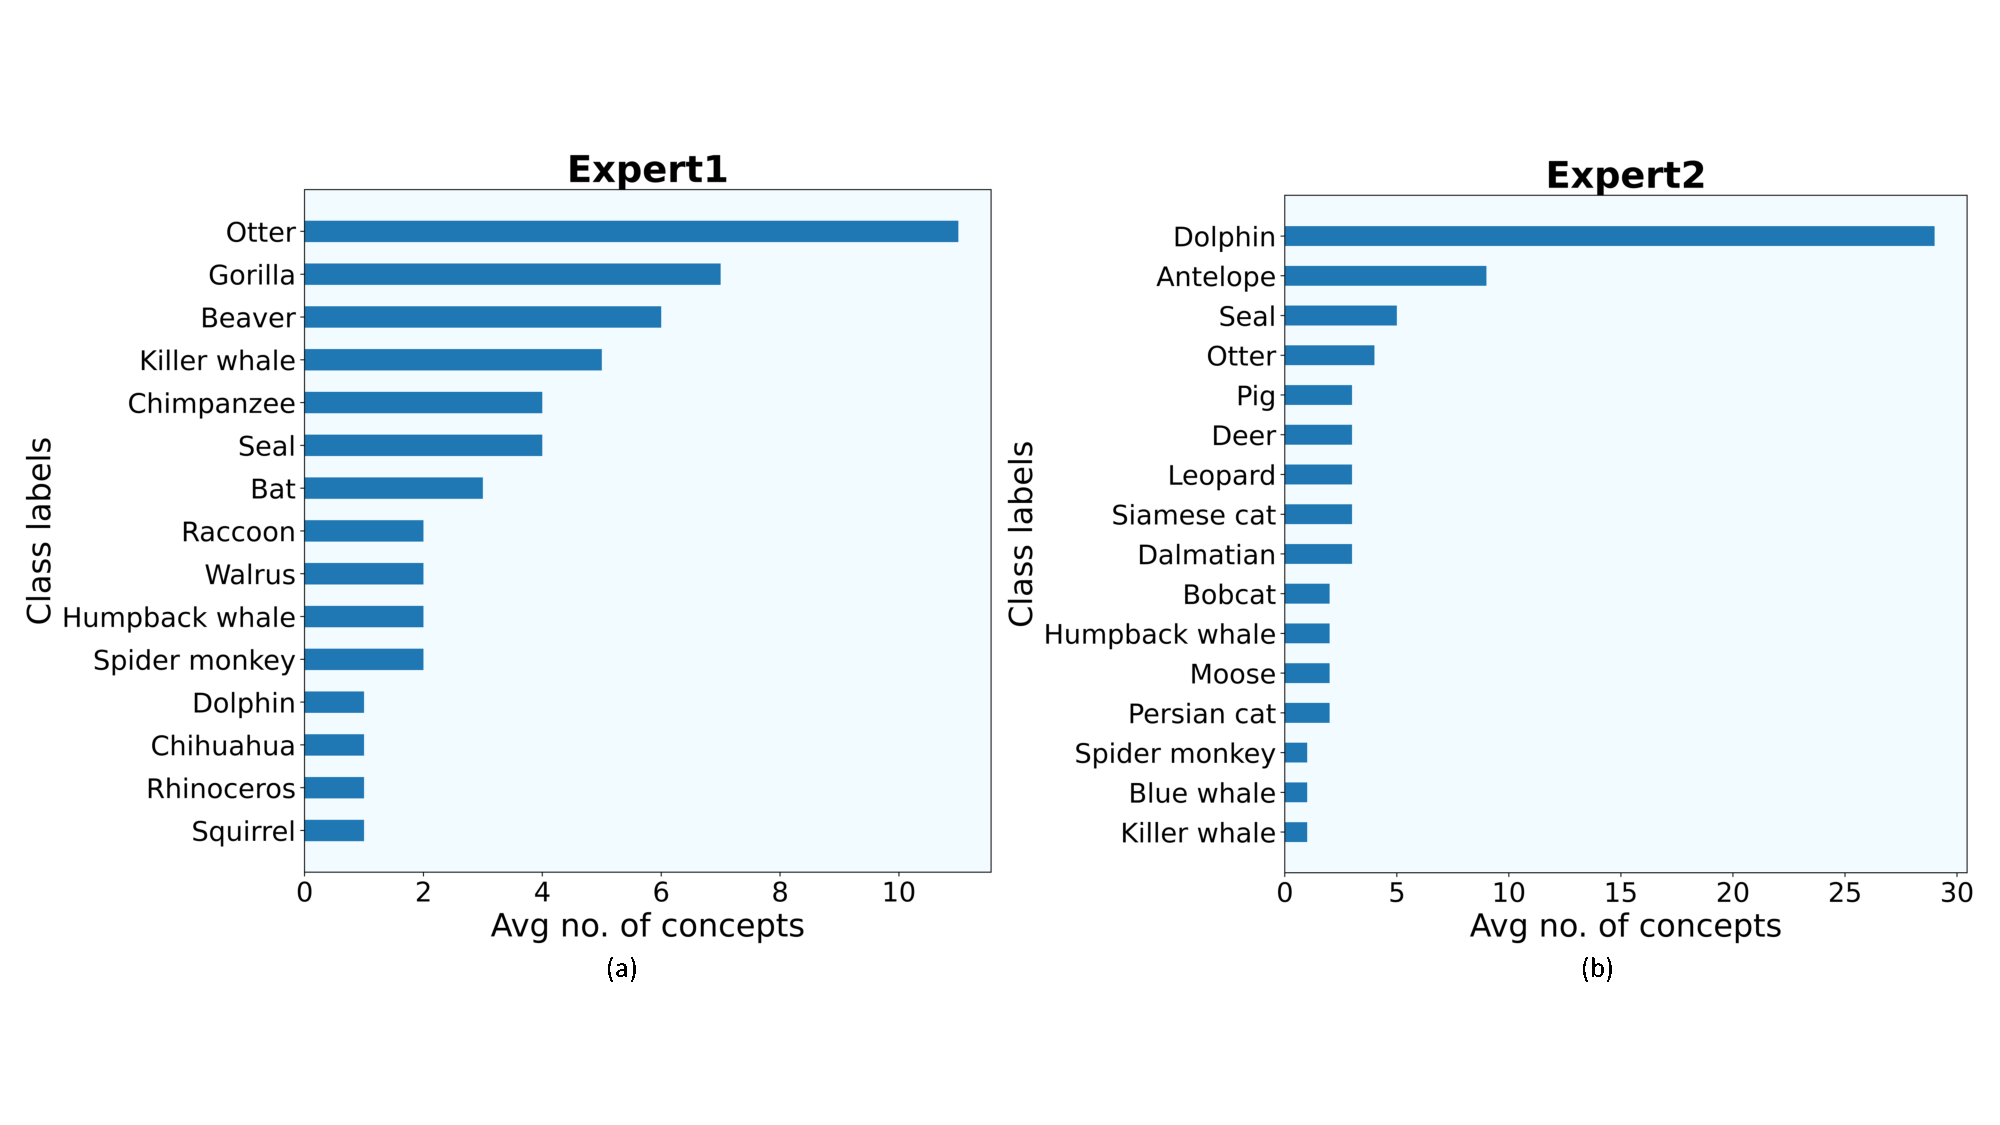
\includegraphics[width=1\textwidth]{figures/Supp/Avg_concept_class_VIT_Awa2_1.pdf} 
%   \label{fig:Awa2_VIT_a}} \\
%   \subfloat{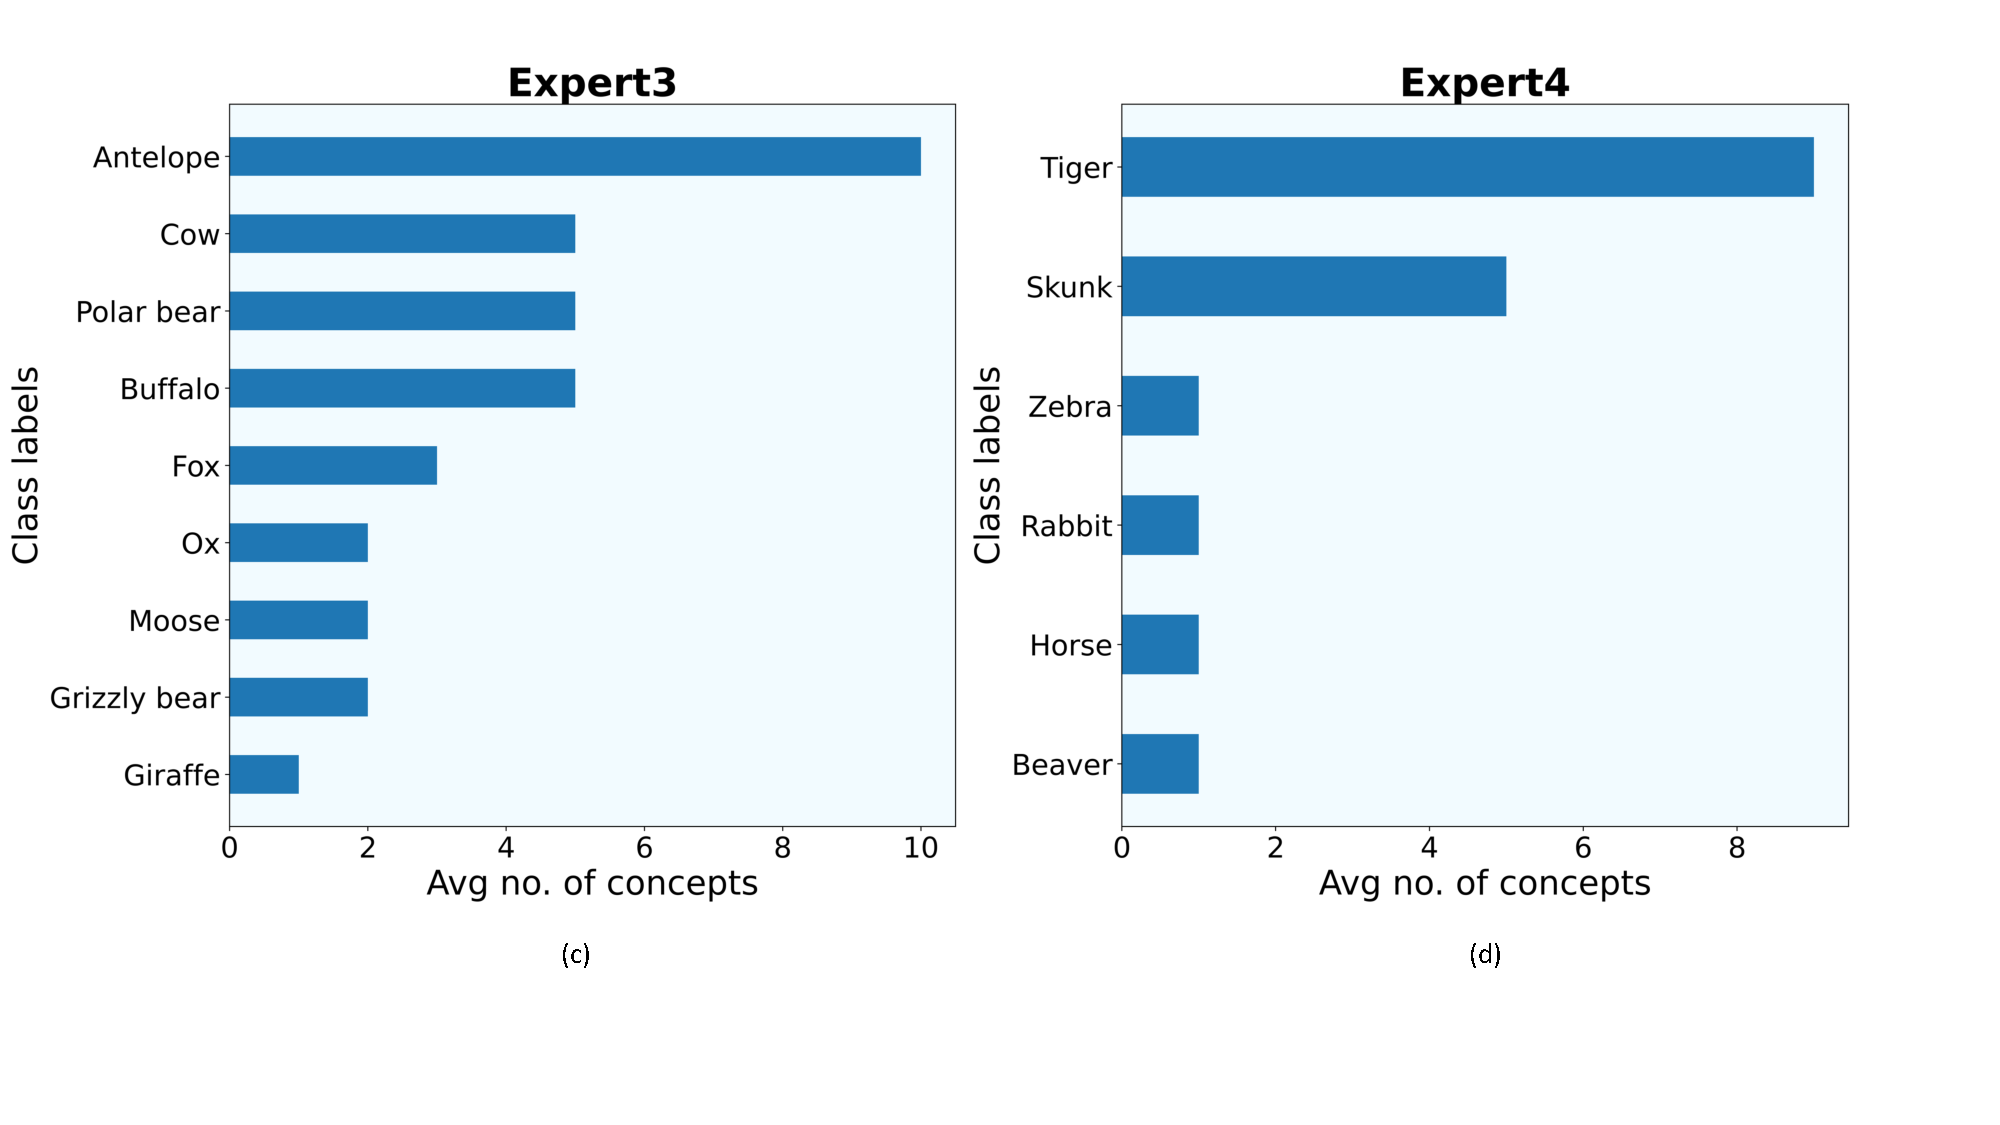
\includegraphics[width=1\textwidth]{figures/Supp/Avg_concept_class_VIT_Awa2_2.pdf} 
%   \label{fig:Awa2_VIT_b}} \\
%   \subfloat{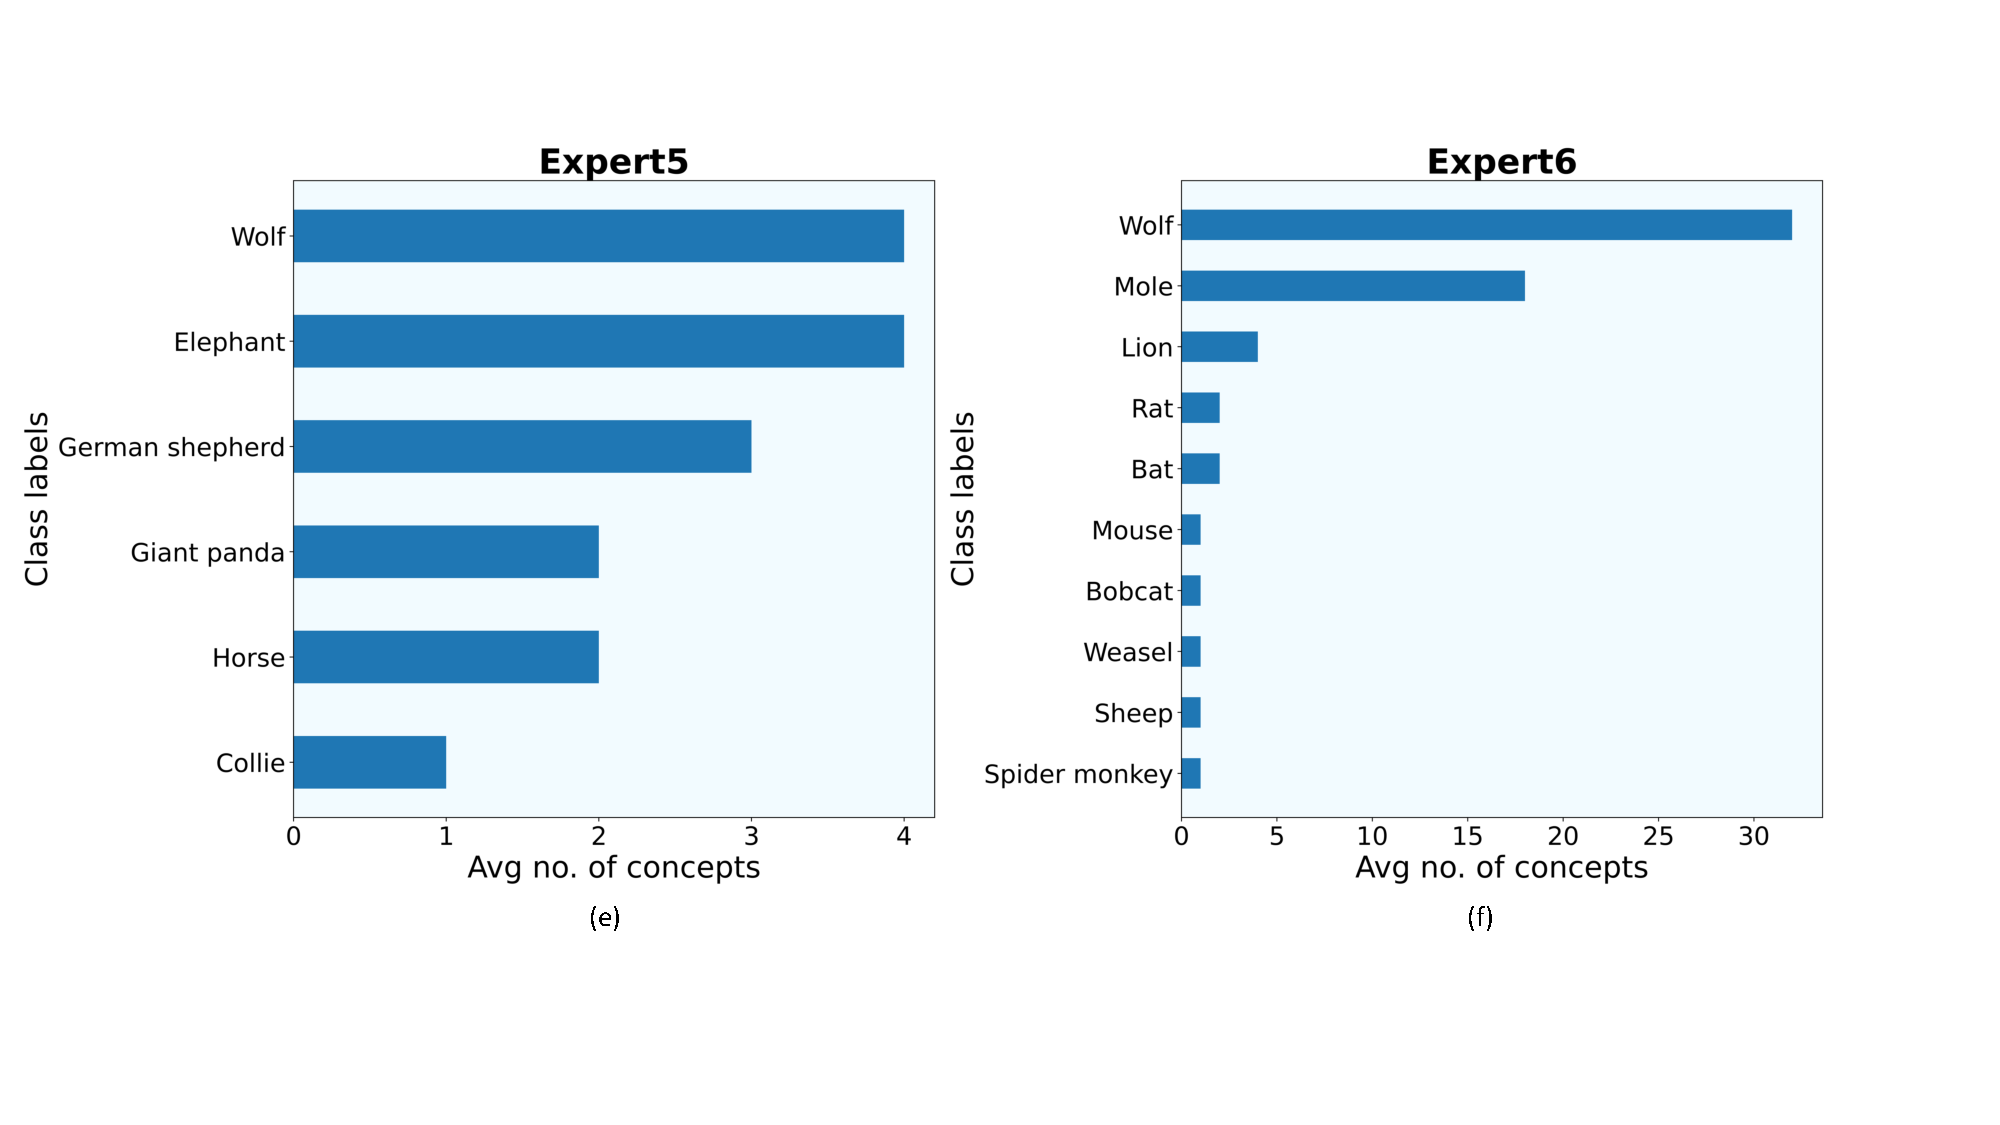
\includegraphics[width=1\textwidth]{figures/Supp/Avg_concept_class_VIT_Awa2_3.pdf} 
%   \label{fig:Awa2_VIT_c}} \\
%   \caption{Class labels (Animal species) vs avg concepts using VIT as backbone for Awa2. Each bar in this plot indicates the average number concepts required to explain each sample of that animal species correctly. \textcolor{red}{For example according to (a) expert1 requires approximately 80 concepts to explain an instance of ``Otter''}.} 
%   \label{fig:Awa2_VIT_concept}
% \end{figure}

\subsection{Computational performance }
\label{app:validate_concepts}
\cref{fig:flops} shows the computational performance compared to the Blackbox. Though in MoIE, we sequentially learn the experts and the residuals, they take less computational resources than the Blackbox. The experts are shallow neural networks. Also, we only update the classification layer ($h$) for the residuals, so it takes such less time. The Flops in the Y axis are computed as Flop of (forward propagation + backward propagation) $\times$ (minibatch size) $\times$ (no of training epochs).
We use the Pytorch profiler package to monitor the flops.

\begin{figure*}[h]
\centering
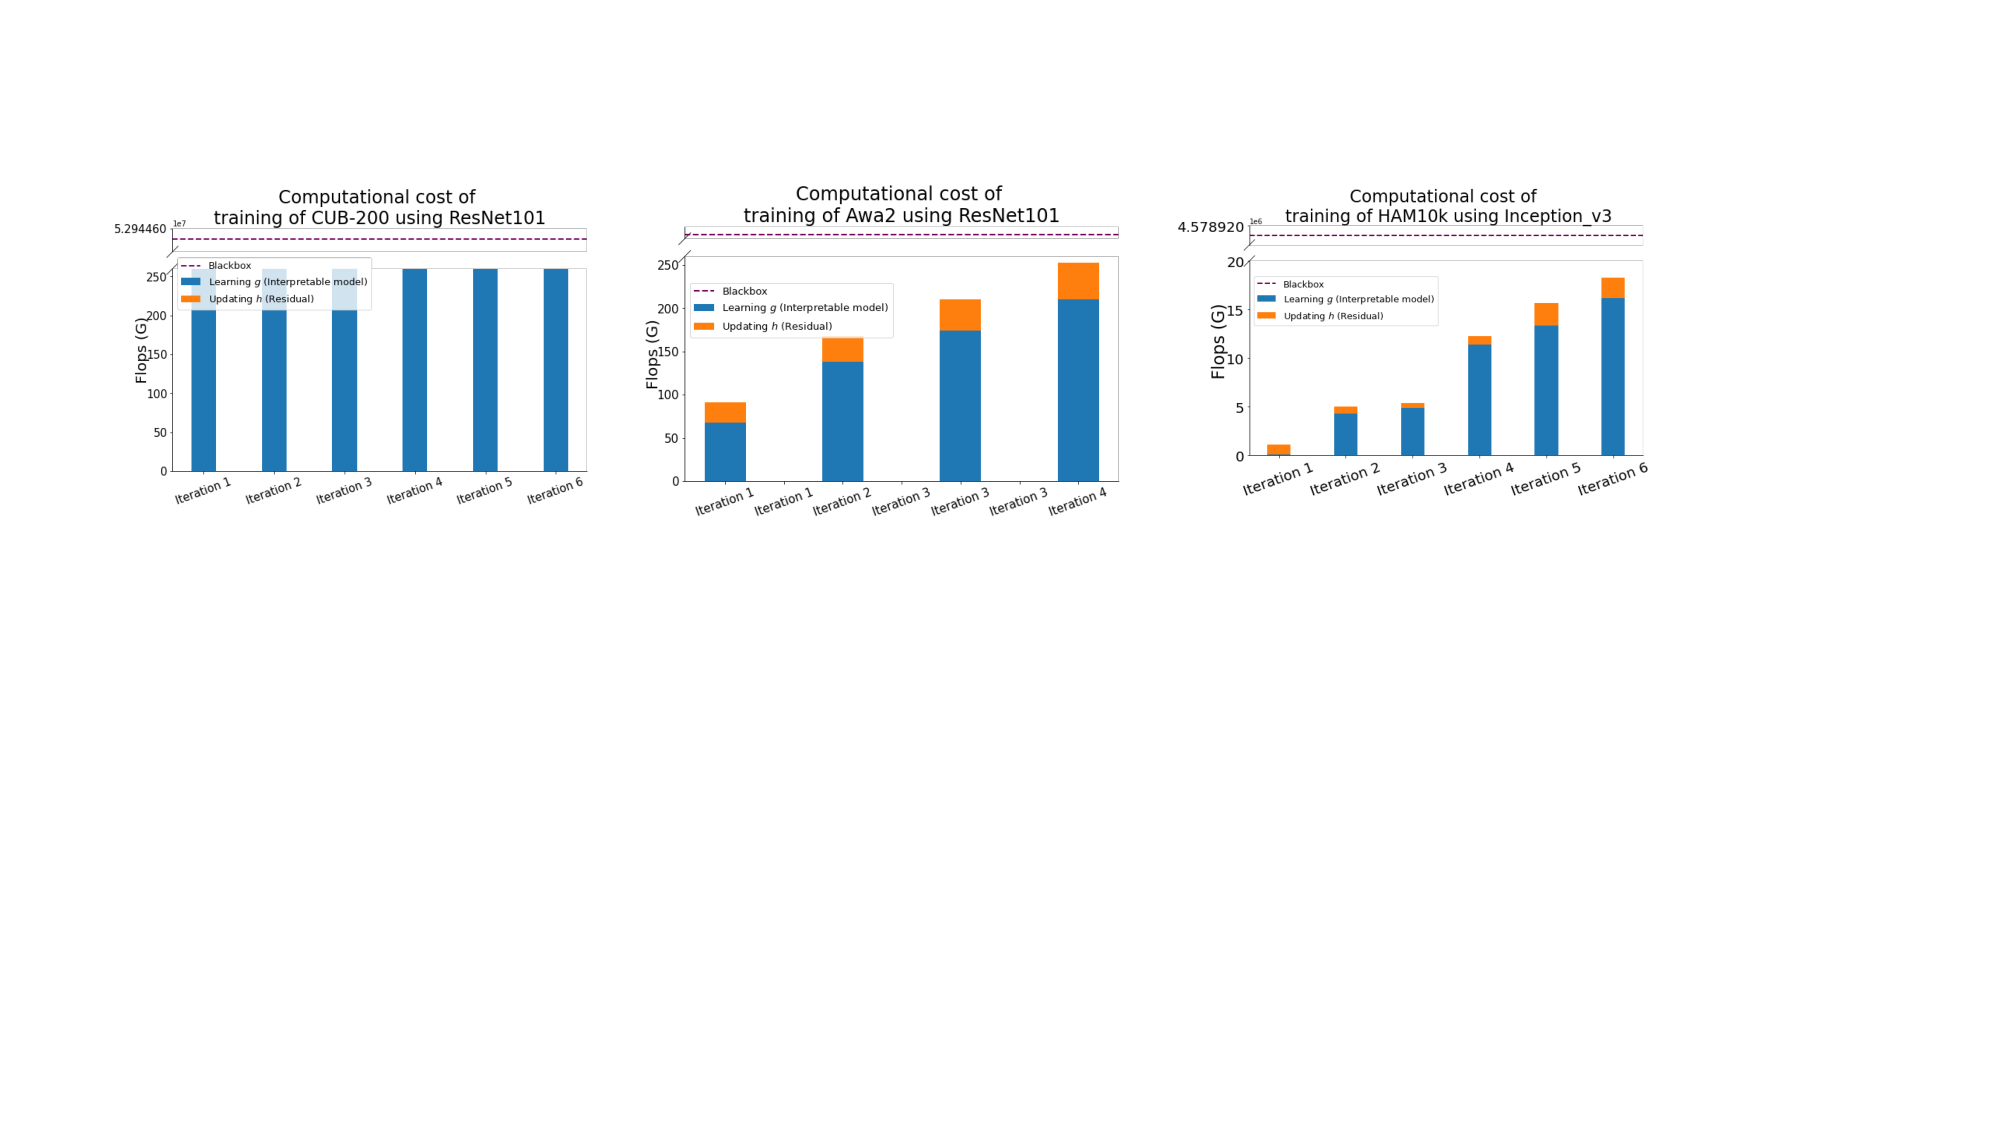
\includegraphics[width=1.0\textwidth]
{figures/Supp/Flops.pdf}
\caption{Flops vs. iteration for MoIE and the Blackbox. The dotted line in the figure represents the flops taken by the blackbox.}
\label{fig:flops}
\end{figure*}


% \subsubsection{Diversity of explanations for SIIM-ISIC}
% \label{app:local_isic}
% \begin{figure*}[h]
\centering
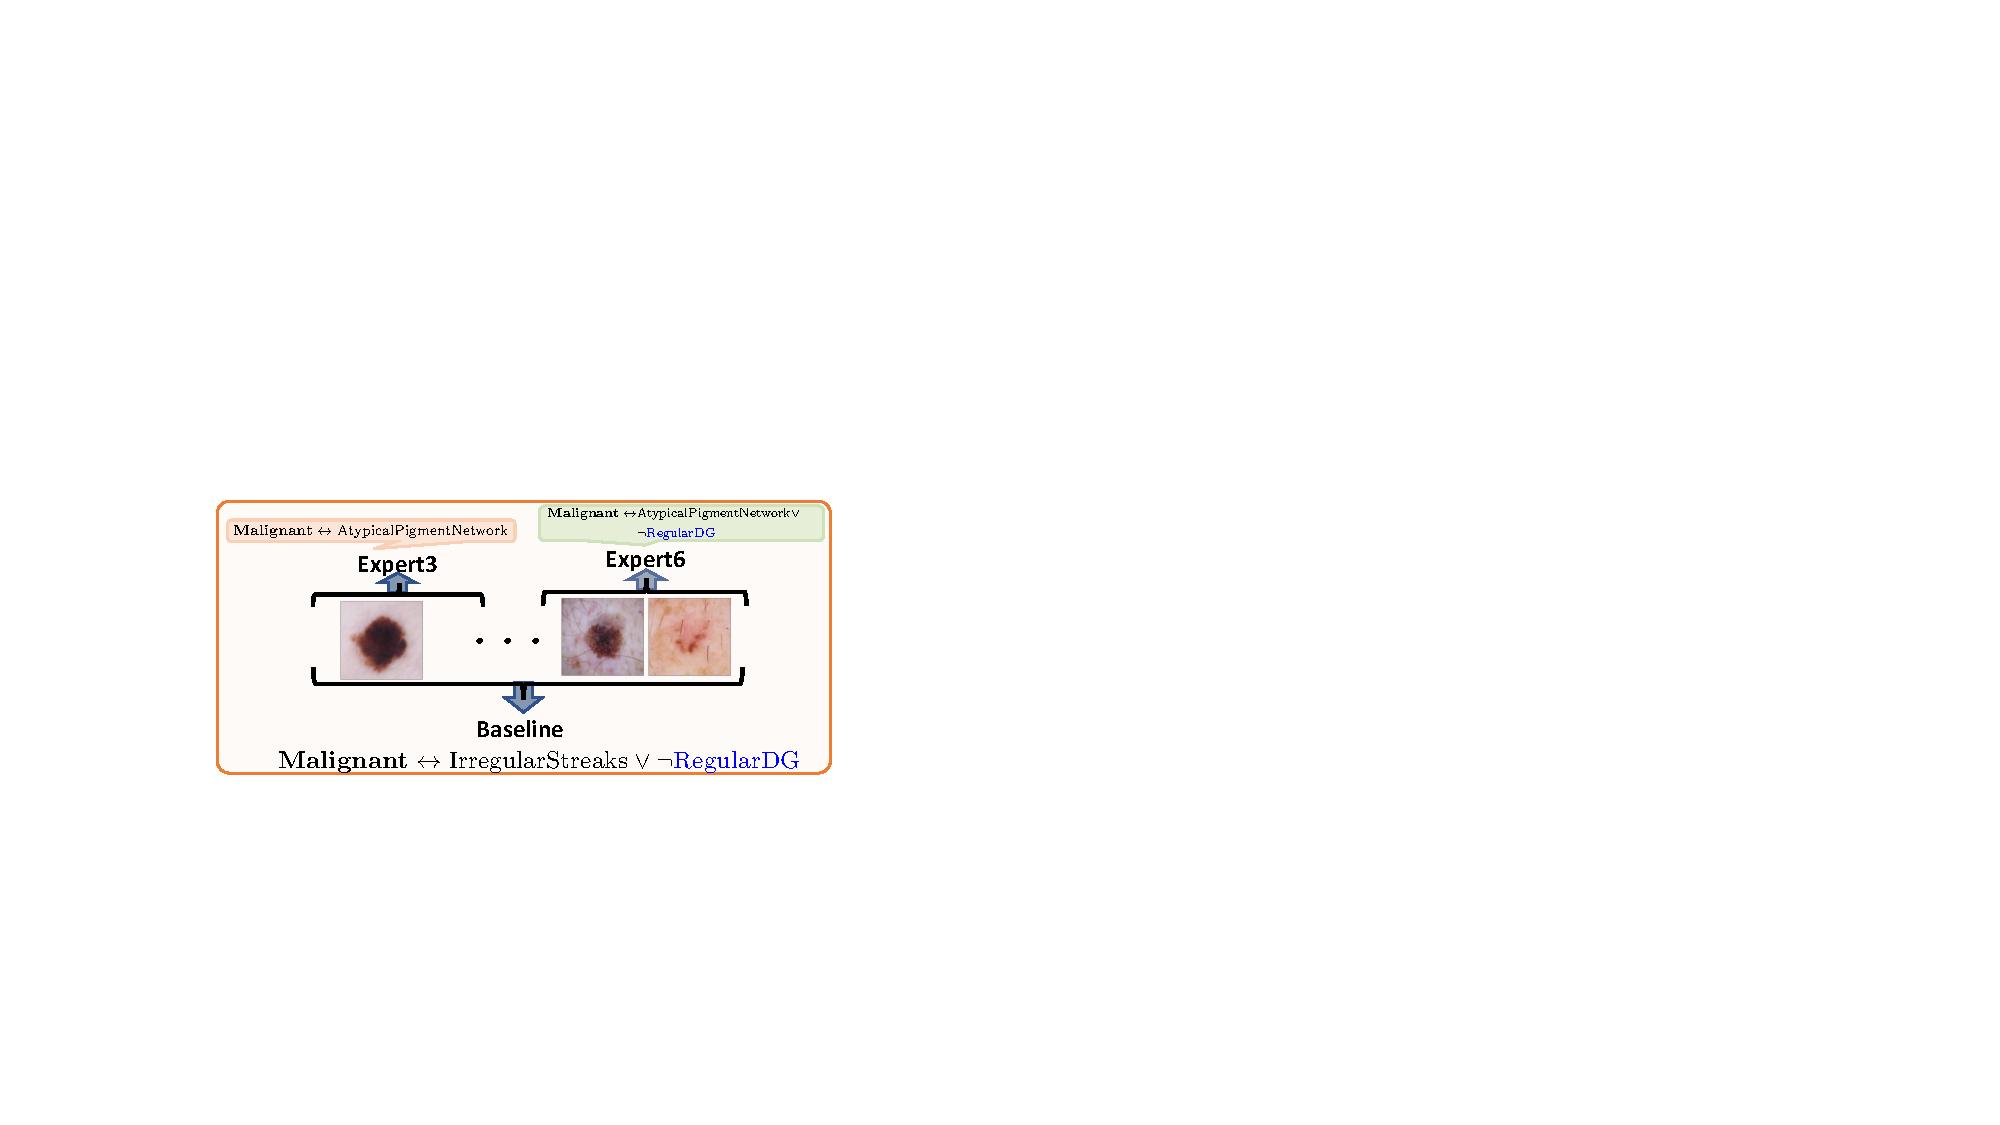
\includegraphics[width=\columnwidth]{figures/Supp/Local_isic.pdf}
\vspace{-10pt}
\caption{Flexibility of FOL explanations by VIT-derived MoIE  MoIE and  the baselines for Awa2 dataset. We compare the FOL for different MoIE experts with the baselines to classify (a) Otter (b) Horse in Awa2For example in figure (b), the baseline's FOL constitutes identical concepts to distinguish all the samples ``Horse''. However, expert4 classifies ``Horse'' with \textit{smelly} as the identifying concept for the instances covered by it. Similarly expert5 classifies the same ``Horse'' using \textit{longneck} and \textit{fields}.  We highlight the shared concepts between the experts and the baselines.}
\label{fig:local_awa2}
\vspace{-2.5pt}
\end{figure*}

xxxxx





%%%%%%%%%%%%%%%%%%%%%%%%%%%%%%%%%%%%%%%%%%%%%%%%%%%%%%%%%%%%%%%%%%%%%%%%%%%%%%%
%%%%%%%%%%%%%%%%%%%%%%%%%%%%%%%%%%%%%%%%%%%%%%%%%%%%%%%%%%%%%%%%%%%%%%%%%%%%%%%


\end{document}



% This document was modified from the file originally made available by
% Pat Langley and Andrea Danyluk for ICML-2K. This version was created
% by Iain Murray in 2018, and modified by Alexandre Bouchard in
% 2019 and 2021 and by Csaba Szepesvari, Gang Niu and Sivan Sabato in 2022.
% Modified again in 2023 by Sivan Sabato and Jonathan Scarlett.
% Previous contributors include Dan Roy, Lise Getoor and Tobias
% Scheffer, which was slightly modified from the 2010 version by
% Thorsten Joachims & Johannes Fuernkranz, slightly modified from the
% 2009 version by Kiri Wagstaff and Sam Roweis's 2008 version, which is
% slightly modified from Prasad Tadepalli's 2007 version which is a
% lightly changed version of the previous year's version by Andrew
% Moore, which was in turn edited from those of Kristian Kersting and
% Codrina Lauth. Alex Smola contributed to the algorithmic style files.
